% !TeX encoding = UTF-8
% !TeX root = V39_Spectroscopy_Rb.tex
% !TeX spellcheck = en_US

\section{Execution} % Experimental setup ?

We use a laser diode which emits in the range of 740-790 nm \cite{lit:diode} to excite the \textsf{Rb} transitions.

The laser diode is driven by a current $I(t)$ consisting of a constant base to select the emitted wavelength plus a saw tooth signal to sweep through the relevant part of the spectrum. As the change in wavelength $\Delta \lambda \propto \Delta I$ and $\Delta \nu \approx - \frac{c}{\lambda^2}\Delta \lambda$ for $\Delta \nu \ll \nu$, we can directly transfer this spectrum into the frequency space.\\
As the rubidium D2 line is around $380 \,\tera\hertz$ and the observed frequency range spans only 7\,GHz, we can safely use this approximation.

\subsection{Absorption spectroscopy}

For absorption spectroscopy, the beam is weakened before entering the gas cuvette by means of a two polarization filters. This is necessary as the full beam would not only saturate the transitions but also threaten to damage the photo diode.

By adjusting the diode current, the wavelength ramp is chosen so that the spectrum fits on a segment between two mode hops of the laser.

When switching to the saturation spectroscopy, the beam passes through the cuvette (pump beam to saturate the transitions) and a small part of it is reflected back (probe beam). In order to couple out the probe beam with a beam splitter, we place a $\lambda/4$ waveplate between the cuvette and the mirror at 45\degree which the beam passes twice, thus changing polarization by 90\degree.

In the saturation mode, we measure both a full spectrum as well as detail spectra of the lamb dips on each of the peaks.

\subsection{Frequency modulation spectroscopy}
The laser is modulated with a signal
\begin{equation}
 U_\text{mod} = U_1 \sin(\omega t) \qquad \omega = 2 \pi \nu,~ \nu = 0.1\,\mega\hertz
\end{equation}

The laser frequency follows, shifting by $\Delta \nu$ each period.

The signal at the photodiode thus varies by $\Delta I \propto \ddp{I}{\nu} \cdt \Delta \nu$, allowing us to obtain the first derivative of the spectrum.

This measurement is done once for each of the four peaks.


\newpage
\section{Analysis}
\subsection{Absorption spectroscopy}

It has to be noted that, as the original spectrum is plotted against the wavelength, the numbering of the peaks is inverse to the order which would have been used on a frequency spectrum -- peak 4 corresponds to the lowest frequency, which we set to $0 \,\hertz$.

As the screenshots taken from the oscilloscope aren't sufficient to obtain precise information (cp. figure \ref{fig:oszi}), we analyzed our data with Matlab.

While we measure the voltage $U_\text{photo}~[\volt]$ from the photo diode in function of the time $t~[\milli\second]$, both data sets are only proportional to relevant quantities; we thus will transform these for our plots in the further sections.

It is to be noted that, while figure \ref{fig:absorption} shows the absorption spectrum, one can still see some small indentations near where lamb dips would appear if it were a saturation spectrum. This could either be reflected light acting as a probe beam (unlikely as the main beam is much more powerful) or due to the doppler broadening not completely smearing the hyperfine structure of the excited state.

\begin{figure}[h]
	\centering
	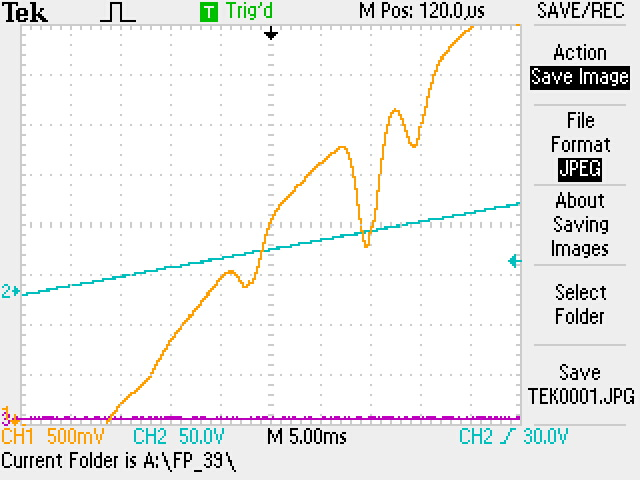
\includegraphics[width=0.95\textwidth]{data/TEK0001.jpg}
	\caption{Screenshot of the oscilloscope showing the current ramp $I(t)$ and the spectrum.}
	\label{fig:oszi}
	\vspace{-2em}
\end{figure}

\begin{figure}[p]
	\centering
	% This file was created by matlab2tikz.
% Minimal pgfplots version: 1.3
%
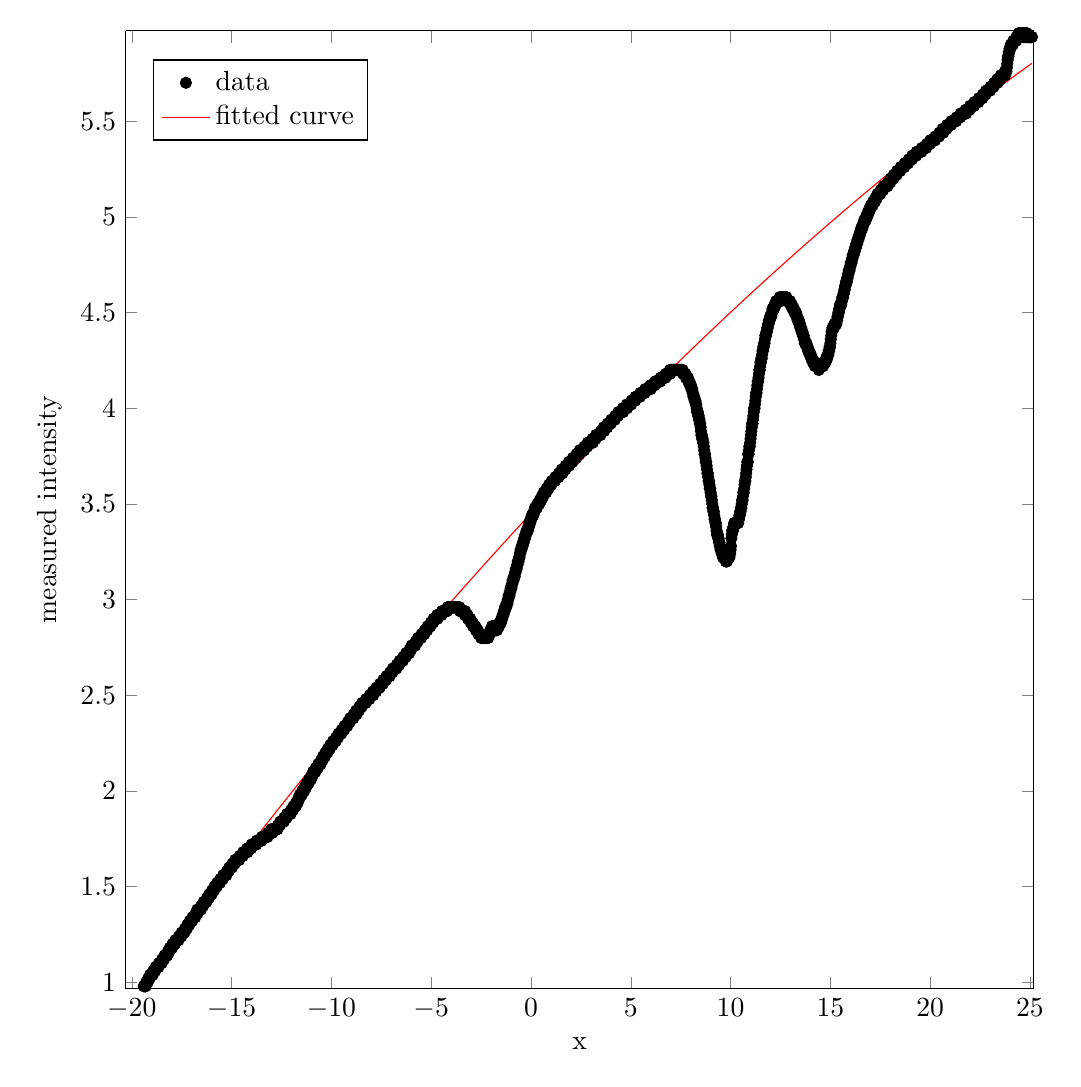
\begin{tikzpicture}

\begin{axis}[%
width=0.95092\textwidth,
height=1.003178\textwidth,
at={(0\textwidth,0\textwidth)},
scale only axis,
separate axis lines,
every outer x axis line/.append style={black},
every x tick label/.append style={font=\color{black}},
xmin=-20.3077975376197,
xmax=25.1778385772914,
xlabel={x},
every outer y axis line/.append style={black},
every y tick label/.append style={font=\color{black}},
ymin=0.967616580310881,
ymax=5.97279792746114,
ylabel={measured intensity},
legend style={at={(0.03,0.97)},anchor=north west,legend cell align=left,align=left,fill=white}
]
\addplot [color=black,only marks,mark=*,mark options={solid}]
  table[row sep=crcr]{%
-19.76	0.92\\
-19.74	0.92\\
-19.72	0.92\\
-19.7	0.92\\
-19.68	0.92\\
-19.66	0.94\\
-19.64	0.94\\
-19.62	0.94\\
-19.6	0.94\\
-19.58	0.94\\
-19.56	0.94\\
-19.54	0.94\\
-19.52	0.96\\
-19.5	0.96\\
-19.48	0.96\\
-19.46	0.96\\
-19.44	0.96\\
-19.42	0.96\\
-19.4	0.98\\
-19.38	0.98\\
-19.36	0.98\\
-19.34	0.98\\
-19.32	0.98\\
-19.3	0.98\\
-19.28	1\\
-19.26	1\\
-19.24	1\\
-19.22	1\\
-19.2	1\\
-19.18	1.02\\
-19.16	1.02\\
-19.14	1.02\\
-19.12	1.02\\
-19.1	1.02\\
-19.08	1.04\\
-19.06	1.04\\
-19.04	1.04\\
-19.02	1.04\\
-19	1.04\\
-18.98	1.04\\
-18.96	1.04\\
-18.94	1.04\\
-18.92	1.06\\
-18.9	1.06\\
-18.88	1.06\\
-18.86	1.06\\
-18.84	1.06\\
-18.82	1.06\\
-18.8	1.08\\
-18.78	1.08\\
-18.76	1.08\\
-18.74	1.08\\
-18.72	1.08\\
-18.7	1.08\\
-18.68	1.08\\
-18.66	1.08\\
-18.64	1.1\\
-18.62	1.1\\
-18.6	1.1\\
-18.58	1.1\\
-18.56	1.1\\
-18.54	1.1\\
-18.52	1.1\\
-18.5	1.1\\
-18.48	1.12\\
-18.46	1.12\\
-18.44	1.12\\
-18.42	1.12\\
-18.4	1.12\\
-18.38	1.12\\
-18.36	1.14\\
-18.34	1.14\\
-18.32	1.14\\
-18.3	1.14\\
-18.28	1.14\\
-18.26	1.14\\
-18.24	1.14\\
-18.22	1.14\\
-18.2	1.16\\
-18.18	1.16\\
-18.16	1.16\\
-18.14	1.16\\
-18.12	1.16\\
-18.1	1.18\\
-18.08	1.18\\
-18.06	1.18\\
-18.04	1.18\\
-18.02	1.18\\
-18	1.18\\
-17.98	1.18\\
-17.96	1.2\\
-17.94	1.2\\
-17.92	1.2\\
-17.9	1.2\\
-17.88	1.2\\
-17.86	1.2\\
-17.84	1.2\\
-17.82	1.22\\
-17.8	1.22\\
-17.78	1.22\\
-17.76	1.22\\
-17.74	1.22\\
-17.72	1.22\\
-17.7	1.22\\
-17.68	1.22\\
-17.66	1.22\\
-17.64	1.24\\
-17.62	1.24\\
-17.6	1.24\\
-17.58	1.24\\
-17.56	1.24\\
-17.54	1.24\\
-17.52	1.24\\
-17.5	1.26\\
-17.48	1.26\\
-17.46	1.26\\
-17.44	1.26\\
-17.42	1.26\\
-17.4	1.26\\
-17.38	1.26\\
-17.36	1.26\\
-17.34	1.28\\
-17.32	1.28\\
-17.3	1.28\\
-17.28	1.28\\
-17.26	1.28\\
-17.24	1.28\\
-17.22	1.3\\
-17.2	1.3\\
-17.18	1.3\\
-17.16	1.3\\
-17.14	1.3\\
-17.12	1.3\\
-17.1	1.32\\
-17.08	1.32\\
-17.06	1.32\\
-17.04	1.32\\
-17.02	1.32\\
-17	1.32\\
-16.98	1.32\\
-16.96	1.34\\
-16.94	1.34\\
-16.92	1.34\\
-16.9	1.34\\
-16.88	1.34\\
-16.86	1.34\\
-16.84	1.34\\
-16.82	1.34\\
-16.8	1.36\\
-16.78	1.36\\
-16.76	1.36\\
-16.74	1.36\\
-16.72	1.38\\
-16.7	1.36\\
-16.68	1.38\\
-16.66	1.38\\
-16.64	1.38\\
-16.62	1.38\\
-16.6	1.38\\
-16.58	1.38\\
-16.56	1.38\\
-16.54	1.38\\
-16.52	1.4\\
-16.5	1.4\\
-16.48	1.4\\
-16.46	1.4\\
-16.44	1.4\\
-16.42	1.4\\
-16.4	1.42\\
-16.38	1.42\\
-16.36	1.42\\
-16.34	1.42\\
-16.32	1.42\\
-16.3	1.42\\
-16.28	1.42\\
-16.26	1.42\\
-16.24	1.44\\
-16.22	1.44\\
-16.2	1.44\\
-16.18	1.44\\
-16.16	1.44\\
-16.14	1.44\\
-16.12	1.46\\
-16.1	1.46\\
-16.08	1.46\\
-16.06	1.46\\
-16.04	1.46\\
-16.02	1.46\\
-16	1.46\\
-15.98	1.48\\
-15.96	1.48\\
-15.94	1.48\\
-15.92	1.48\\
-15.9	1.48\\
-15.88	1.48\\
-15.86	1.5\\
-15.84	1.5\\
-15.82	1.5\\
-15.8	1.5\\
-15.78	1.5\\
-15.76	1.5\\
-15.74	1.5\\
-15.72	1.52\\
-15.7	1.52\\
-15.68	1.52\\
-15.66	1.52\\
-15.64	1.52\\
-15.62	1.52\\
-15.6	1.52\\
-15.58	1.52\\
-15.56	1.54\\
-15.54	1.54\\
-15.52	1.54\\
-15.5	1.54\\
-15.48	1.54\\
-15.46	1.54\\
-15.44	1.54\\
-15.42	1.56\\
-15.4	1.56\\
-15.38	1.56\\
-15.36	1.56\\
-15.34	1.56\\
-15.32	1.56\\
-15.3	1.56\\
-15.28	1.56\\
-15.26	1.56\\
-15.24	1.58\\
-15.22	1.58\\
-15.2	1.58\\
-15.18	1.58\\
-15.16	1.58\\
-15.14	1.58\\
-15.12	1.6\\
-15.1	1.6\\
-15.08	1.6\\
-15.06	1.6\\
-15.04	1.6\\
-15.02	1.6\\
-15	1.6\\
-14.98	1.6\\
-14.96	1.62\\
-14.94	1.62\\
-14.92	1.62\\
-14.9	1.62\\
-14.88	1.62\\
-14.86	1.62\\
-14.84	1.62\\
-14.82	1.64\\
-14.8	1.64\\
-14.78	1.64\\
-14.76	1.64\\
-14.74	1.64\\
-14.72	1.64\\
-14.7	1.64\\
-14.68	1.64\\
-14.66	1.64\\
-14.64	1.64\\
-14.62	1.64\\
-14.6	1.66\\
-14.58	1.66\\
-14.56	1.66\\
-14.54	1.66\\
-14.52	1.66\\
-14.5	1.66\\
-14.48	1.66\\
-14.46	1.66\\
-14.44	1.66\\
-14.42	1.68\\
-14.4	1.68\\
-14.38	1.68\\
-14.36	1.68\\
-14.34	1.68\\
-14.32	1.68\\
-14.3	1.68\\
-14.28	1.68\\
-14.26	1.68\\
-14.24	1.68\\
-14.22	1.7\\
-14.2	1.68\\
-14.18	1.7\\
-14.16	1.7\\
-14.14	1.7\\
-14.12	1.7\\
-14.1	1.7\\
-14.08	1.7\\
-14.06	1.7\\
-14.04	1.7\\
-14.02	1.7\\
-14	1.72\\
-13.98	1.72\\
-13.96	1.72\\
-13.94	1.72\\
-13.92	1.72\\
-13.9	1.72\\
-13.88	1.72\\
-13.86	1.72\\
-13.84	1.72\\
-13.82	1.72\\
-13.8	1.72\\
-13.78	1.72\\
-13.76	1.72\\
-13.74	1.74\\
-13.72	1.74\\
-13.7	1.74\\
-13.68	1.74\\
-13.66	1.74\\
-13.64	1.74\\
-13.62	1.74\\
-13.6	1.74\\
-13.58	1.74\\
-13.56	1.74\\
-13.54	1.74\\
-13.52	1.74\\
-13.5	1.74\\
-13.48	1.76\\
-13.46	1.76\\
-13.44	1.76\\
-13.42	1.76\\
-13.4	1.76\\
-13.38	1.76\\
-13.36	1.76\\
-13.34	1.76\\
-13.32	1.76\\
-13.3	1.76\\
-13.28	1.76\\
-13.26	1.76\\
-13.24	1.76\\
-13.22	1.76\\
-13.2	1.76\\
-13.18	1.78\\
-13.16	1.78\\
-13.14	1.78\\
-13.12	1.78\\
-13.1	1.78\\
-13.08	1.78\\
-13.06	1.78\\
-13.04	1.78\\
-13.02	1.8\\
-13	1.78\\
-12.98	1.8\\
-12.96	1.78\\
-12.94	1.8\\
-12.92	1.8\\
-12.9	1.8\\
-12.88	1.8\\
-12.86	1.8\\
-12.84	1.8\\
-12.82	1.8\\
-12.8	1.8\\
-12.78	1.8\\
-12.76	1.8\\
-12.74	1.8\\
-12.72	1.8\\
-12.7	1.8\\
-12.68	1.82\\
-12.66	1.82\\
-12.64	1.82\\
-12.62	1.82\\
-12.6	1.82\\
-12.58	1.82\\
-12.56	1.84\\
-12.54	1.84\\
-12.52	1.84\\
-12.5	1.84\\
-12.48	1.84\\
-12.46	1.84\\
-12.44	1.84\\
-12.42	1.84\\
-12.4	1.84\\
-12.38	1.84\\
-12.36	1.86\\
-12.34	1.86\\
-12.32	1.86\\
-12.3	1.86\\
-12.28	1.86\\
-12.26	1.86\\
-12.24	1.86\\
-12.22	1.88\\
-12.2	1.88\\
-12.18	1.88\\
-12.16	1.88\\
-12.14	1.88\\
-12.12	1.88\\
-12.1	1.88\\
-12.08	1.88\\
-12.06	1.88\\
-12.04	1.88\\
-12.02	1.9\\
-12	1.9\\
-11.98	1.9\\
-11.96	1.9\\
-11.94	1.9\\
-11.92	1.9\\
-11.9	1.92\\
-11.88	1.92\\
-11.86	1.92\\
-11.84	1.92\\
-11.82	1.92\\
-11.8	1.92\\
-11.78	1.92\\
-11.76	1.94\\
-11.74	1.94\\
-11.72	1.94\\
-11.7	1.94\\
-11.68	1.94\\
-11.66	1.96\\
-11.64	1.96\\
-11.62	1.96\\
-11.6	1.96\\
-11.58	1.98\\
-11.56	1.98\\
-11.54	1.98\\
-11.52	1.98\\
-11.5	1.98\\
-11.48	1.98\\
-11.46	2\\
-11.44	2\\
-11.42	2\\
-11.4	2\\
-11.38	2\\
-11.36	2\\
-11.34	2.02\\
-11.32	2.02\\
-11.3	2.02\\
-11.28	2.02\\
-11.26	2.02\\
-11.24	2.04\\
-11.22	2.04\\
-11.2	2.04\\
-11.18	2.04\\
-11.16	2.04\\
-11.14	2.04\\
-11.12	2.06\\
-11.1	2.06\\
-11.08	2.06\\
-11.06	2.06\\
-11.04	2.06\\
-11.02	2.06\\
-11	2.08\\
-10.98	2.08\\
-10.96	2.08\\
-10.94	2.08\\
-10.92	2.1\\
-10.9	2.1\\
-10.88	2.1\\
-10.86	2.1\\
-10.84	2.1\\
-10.82	2.1\\
-10.8	2.1\\
-10.78	2.12\\
-10.76	2.12\\
-10.74	2.12\\
-10.72	2.12\\
-10.7	2.12\\
-10.68	2.12\\
-10.66	2.14\\
-10.64	2.14\\
-10.62	2.14\\
-10.6	2.14\\
-10.58	2.14\\
-10.56	2.14\\
-10.54	2.14\\
-10.52	2.16\\
-10.5	2.16\\
-10.48	2.16\\
-10.46	2.16\\
-10.44	2.16\\
-10.42	2.18\\
-10.4	2.18\\
-10.38	2.18\\
-10.36	2.18\\
-10.34	2.18\\
-10.32	2.18\\
-10.3	2.2\\
-10.28	2.2\\
-10.26	2.2\\
-10.24	2.2\\
-10.22	2.2\\
-10.2	2.2\\
-10.18	2.22\\
-10.16	2.22\\
-10.14	2.22\\
-10.12	2.22\\
-10.1	2.22\\
-10.08	2.22\\
-10.06	2.24\\
-10.04	2.24\\
-10.02	2.24\\
-10	2.24\\
-9.98	2.24\\
-9.96	2.24\\
-9.94	2.24\\
-9.92	2.26\\
-9.9	2.26\\
-9.88	2.26\\
-9.86	2.26\\
-9.84	2.26\\
-9.82	2.26\\
-9.8	2.26\\
-9.78	2.26\\
-9.76	2.28\\
-9.74	2.28\\
-9.72	2.28\\
-9.7	2.28\\
-9.68	2.28\\
-9.66	2.28\\
-9.64	2.3\\
-9.62	2.3\\
-9.6	2.3\\
-9.58	2.3\\
-9.56	2.3\\
-9.54	2.3\\
-9.52	2.3\\
-9.5	2.3\\
-9.48	2.32\\
-9.46	2.32\\
-9.44	2.32\\
-9.42	2.32\\
-9.4	2.32\\
-9.38	2.32\\
-9.36	2.32\\
-9.34	2.34\\
-9.32	2.34\\
-9.3	2.34\\
-9.28	2.34\\
-9.26	2.34\\
-9.24	2.34\\
-9.22	2.34\\
-9.2	2.34\\
-9.18	2.36\\
-9.16	2.36\\
-9.14	2.36\\
-9.12	2.36\\
-9.1	2.36\\
-9.08	2.36\\
-9.06	2.38\\
-9.04	2.38\\
-9.02	2.38\\
-9	2.38\\
-8.98	2.38\\
-8.96	2.38\\
-8.94	2.38\\
-8.92	2.38\\
-8.9	2.38\\
-8.88	2.4\\
-8.86	2.4\\
-8.84	2.4\\
-8.82	2.4\\
-8.8	2.4\\
-8.78	2.4\\
-8.76	2.42\\
-8.74	2.4\\
-8.72	2.42\\
-8.7	2.42\\
-8.68	2.42\\
-8.66	2.42\\
-8.64	2.42\\
-8.62	2.42\\
-8.6	2.44\\
-8.58	2.44\\
-8.56	2.44\\
-8.54	2.44\\
-8.52	2.44\\
-8.5	2.44\\
-8.48	2.44\\
-8.46	2.46\\
-8.44	2.46\\
-8.42	2.46\\
-8.4	2.46\\
-8.38	2.46\\
-8.36	2.46\\
-8.34	2.46\\
-8.32	2.46\\
-8.3	2.46\\
-8.28	2.46\\
-8.26	2.48\\
-8.24	2.48\\
-8.22	2.48\\
-8.2	2.48\\
-8.18	2.48\\
-8.16	2.48\\
-8.14	2.48\\
-8.12	2.48\\
-8.1	2.48\\
-8.08	2.5\\
-8.06	2.5\\
-8.04	2.5\\
-8.02	2.5\\
-8	2.5\\
-7.98	2.5\\
-7.96	2.5\\
-7.94	2.5\\
-7.92	2.52\\
-7.9	2.5\\
-7.88	2.52\\
-7.86	2.52\\
-7.84	2.52\\
-7.82	2.52\\
-7.8	2.52\\
-7.78	2.52\\
-7.76	2.52\\
-7.74	2.54\\
-7.72	2.54\\
-7.7	2.54\\
-7.68	2.54\\
-7.66	2.54\\
-7.64	2.54\\
-7.62	2.54\\
-7.6	2.54\\
-7.58	2.54\\
-7.56	2.56\\
-7.54	2.56\\
-7.52	2.56\\
-7.5	2.56\\
-7.48	2.56\\
-7.46	2.56\\
-7.44	2.56\\
-7.42	2.56\\
-7.4	2.58\\
-7.38	2.58\\
-7.36	2.58\\
-7.34	2.58\\
-7.32	2.58\\
-7.3	2.58\\
-7.28	2.58\\
-7.26	2.58\\
-7.24	2.6\\
-7.22	2.6\\
-7.2	2.6\\
-7.18	2.6\\
-7.16	2.6\\
-7.14	2.6\\
-7.12	2.6\\
-7.1	2.6\\
-7.08	2.6\\
-7.06	2.62\\
-7.04	2.62\\
-7.02	2.62\\
-7	2.62\\
-6.98	2.62\\
-6.96	2.62\\
-6.94	2.62\\
-6.92	2.64\\
-6.9	2.64\\
-6.88	2.64\\
-6.86	2.64\\
-6.84	2.64\\
-6.82	2.64\\
-6.8	2.64\\
-6.78	2.64\\
-6.76	2.64\\
-6.74	2.64\\
-6.72	2.66\\
-6.7	2.66\\
-6.68	2.66\\
-6.66	2.66\\
-6.64	2.66\\
-6.62	2.66\\
-6.6	2.66\\
-6.58	2.68\\
-6.56	2.68\\
-6.54	2.68\\
-6.52	2.68\\
-6.5	2.68\\
-6.48	2.68\\
-6.46	2.68\\
-6.44	2.68\\
-6.42	2.68\\
-6.4	2.7\\
-6.38	2.7\\
-6.36	2.7\\
-6.34	2.7\\
-6.32	2.7\\
-6.3	2.7\\
-6.28	2.7\\
-6.26	2.72\\
-6.24	2.72\\
-6.22	2.72\\
-6.2	2.72\\
-6.18	2.72\\
-6.16	2.72\\
-6.14	2.72\\
-6.12	2.72\\
-6.1	2.72\\
-6.08	2.74\\
-6.06	2.74\\
-6.04	2.74\\
-6.02	2.74\\
-6	2.74\\
-5.98	2.76\\
-5.96	2.76\\
-5.94	2.76\\
-5.92	2.76\\
-5.9	2.76\\
-5.88	2.76\\
-5.86	2.76\\
-5.84	2.76\\
-5.82	2.76\\
-5.8	2.76\\
-5.78	2.78\\
-5.76	2.78\\
-5.74	2.78\\
-5.72	2.78\\
-5.7	2.78\\
-5.68	2.78\\
-5.66	2.8\\
-5.64	2.8\\
-5.62	2.8\\
-5.6	2.8\\
-5.58	2.8\\
-5.56	2.8\\
-5.54	2.8\\
-5.52	2.8\\
-5.5	2.8\\
-5.48	2.82\\
-5.46	2.82\\
-5.44	2.82\\
-5.42	2.82\\
-5.4	2.82\\
-5.38	2.82\\
-5.36	2.82\\
-5.34	2.82\\
-5.32	2.84\\
-5.3	2.84\\
-5.28	2.84\\
-5.26	2.84\\
-5.24	2.84\\
-5.22	2.84\\
-5.2	2.84\\
-5.18	2.86\\
-5.16	2.86\\
-5.14	2.86\\
-5.12	2.86\\
-5.1	2.86\\
-5.08	2.86\\
-5.06	2.86\\
-5.04	2.86\\
-5.02	2.88\\
-5	2.88\\
-4.98	2.88\\
-4.96	2.88\\
-4.94	2.88\\
-4.92	2.88\\
-4.9	2.88\\
-4.88	2.9\\
-4.86	2.9\\
-4.84	2.9\\
-4.82	2.9\\
-4.8	2.9\\
-4.78	2.9\\
-4.76	2.9\\
-4.74	2.9\\
-4.72	2.9\\
-4.7	2.92\\
-4.68	2.9\\
-4.66	2.92\\
-4.64	2.92\\
-4.62	2.92\\
-4.6	2.92\\
-4.58	2.92\\
-4.56	2.92\\
-4.54	2.92\\
-4.52	2.92\\
-4.5	2.92\\
-4.48	2.92\\
-4.46	2.94\\
-4.44	2.94\\
-4.42	2.94\\
-4.4	2.94\\
-4.38	2.94\\
-4.36	2.94\\
-4.34	2.94\\
-4.32	2.94\\
-4.3	2.94\\
-4.28	2.94\\
-4.26	2.94\\
-4.24	2.94\\
-4.22	2.94\\
-4.2	2.94\\
-4.18	2.96\\
-4.16	2.96\\
-4.14	2.96\\
-4.12	2.96\\
-4.1	2.96\\
-4.08	2.96\\
-4.06	2.96\\
-4.04	2.96\\
-4.02	2.96\\
-4	2.96\\
-3.98	2.96\\
-3.96	2.96\\
-3.94	2.96\\
-3.92	2.96\\
-3.9	2.96\\
-3.88	2.96\\
-3.86	2.96\\
-3.84	2.96\\
-3.82	2.96\\
-3.8	2.96\\
-3.78	2.96\\
-3.76	2.96\\
-3.74	2.96\\
-3.72	2.96\\
-3.7	2.96\\
-3.68	2.96\\
-3.66	2.96\\
-3.64	2.96\\
-3.62	2.96\\
-3.6	2.96\\
-3.58	2.96\\
-3.56	2.94\\
-3.54	2.94\\
-3.52	2.94\\
-3.5	2.94\\
-3.48	2.94\\
-3.46	2.94\\
-3.44	2.94\\
-3.42	2.94\\
-3.4	2.94\\
-3.38	2.94\\
-3.36	2.94\\
-3.34	2.94\\
-3.32	2.92\\
-3.3	2.94\\
-3.28	2.92\\
-3.26	2.92\\
-3.24	2.92\\
-3.22	2.92\\
-3.2	2.92\\
-3.18	2.92\\
-3.16	2.9\\
-3.14	2.9\\
-3.12	2.9\\
-3.1	2.9\\
-3.08	2.9\\
-3.06	2.9\\
-3.04	2.9\\
-3.02	2.88\\
-3	2.88\\
-2.98	2.88\\
-2.96	2.88\\
-2.94	2.88\\
-2.92	2.88\\
-2.9	2.86\\
-2.88	2.86\\
-2.86	2.86\\
-2.84	2.86\\
-2.82	2.86\\
-2.8	2.86\\
-2.78	2.86\\
-2.76	2.84\\
-2.74	2.84\\
-2.72	2.84\\
-2.7	2.84\\
-2.68	2.84\\
-2.66	2.84\\
-2.64	2.82\\
-2.62	2.82\\
-2.6	2.82\\
-2.58	2.82\\
-2.56	2.82\\
-2.54	2.82\\
-2.52	2.82\\
-2.5	2.8\\
-2.48	2.8\\
-2.46	2.8\\
-2.44	2.8\\
-2.42	2.8\\
-2.4	2.8\\
-2.38	2.8\\
-2.36	2.8\\
-2.34	2.8\\
-2.32	2.8\\
-2.3	2.8\\
-2.28	2.8\\
-2.26	2.8\\
-2.24	2.8\\
-2.22	2.8\\
-2.2	2.8\\
-2.18	2.8\\
-2.16	2.8\\
-2.14	2.8\\
-2.12	2.82\\
-2.1	2.82\\
-2.08	2.82\\
-2.06	2.82\\
-2.04	2.84\\
-2.02	2.84\\
-2	2.84\\
-1.98	2.84\\
-1.96	2.86\\
-1.94	2.86\\
-1.92	2.86\\
-1.9	2.86\\
-1.88	2.86\\
-1.86	2.86\\
-1.84	2.86\\
-1.82	2.84\\
-1.8	2.86\\
-1.78	2.84\\
-1.76	2.84\\
-1.74	2.86\\
-1.72	2.86\\
-1.7	2.84\\
-1.68	2.86\\
-1.66	2.86\\
-1.64	2.86\\
-1.62	2.86\\
-1.6	2.86\\
-1.58	2.88\\
-1.56	2.88\\
-1.54	2.88\\
-1.52	2.88\\
-1.5	2.88\\
-1.48	2.9\\
-1.46	2.9\\
-1.44	2.9\\
-1.42	2.92\\
-1.4	2.92\\
-1.38	2.92\\
-1.36	2.94\\
-1.34	2.94\\
-1.32	2.94\\
-1.3	2.96\\
-1.28	2.96\\
-1.26	2.96\\
-1.24	2.96\\
-1.22	2.98\\
-1.2	2.98\\
-1.18	2.98\\
-1.16	3\\
-1.14	3\\
-1.12	3.02\\
-1.1	3.02\\
-1.08	3.02\\
-1.06	3.04\\
-1.04	3.04\\
-1.02	3.06\\
-1	3.06\\
-0.98	3.06\\
-0.96	3.08\\
-0.94	3.08\\
-0.92	3.1\\
-0.9	3.1\\
-0.88	3.1\\
-0.86	3.12\\
-0.84	3.12\\
-0.82	3.12\\
-0.8	3.14\\
-0.78	3.14\\
-0.76	3.16\\
-0.74	3.16\\
-0.72	3.16\\
-0.7	3.18\\
-0.68	3.18\\
-0.66	3.2\\
-0.64	3.2\\
-0.62	3.2\\
-0.6	3.22\\
-0.58	3.22\\
-0.56	3.24\\
-0.54	3.24\\
-0.52	3.26\\
-0.5	3.26\\
-0.48	3.26\\
-0.46	3.28\\
-0.44	3.28\\
-0.42	3.28\\
-0.4	3.3\\
-0.38	3.3\\
-0.36	3.3\\
-0.34	3.32\\
-0.32	3.32\\
-0.3	3.32\\
-0.28	3.34\\
-0.26	3.34\\
-0.24	3.34\\
-0.22	3.36\\
-0.2	3.36\\
-0.18	3.36\\
-0.16	3.36\\
-0.14	3.38\\
-0.12	3.38\\
-0.1	3.38\\
-0.08	3.4\\
-0.06	3.4\\
-0.04	3.4\\
-0.02	3.42\\
-0	3.42\\
0.02	3.42\\
0.04	3.44\\
0.06	3.44\\
0.08	3.44\\
0.1	3.44\\
0.12	3.44\\
0.14	3.46\\
0.16	3.46\\
0.18	3.46\\
0.2	3.48\\
0.22	3.48\\
0.24	3.48\\
0.26	3.48\\
0.28	3.48\\
0.3	3.48\\
0.32	3.5\\
0.34	3.5\\
0.36	3.5\\
0.38	3.5\\
0.4	3.5\\
0.42	3.5\\
0.44	3.52\\
0.46	3.52\\
0.48	3.52\\
0.5	3.52\\
0.52	3.52\\
0.54	3.54\\
0.56	3.54\\
0.58	3.54\\
0.6	3.54\\
0.62	3.54\\
0.64	3.56\\
0.66	3.56\\
0.68	3.56\\
0.7	3.56\\
0.72	3.56\\
0.74	3.56\\
0.76	3.56\\
0.78	3.58\\
0.8	3.58\\
0.82	3.58\\
0.84	3.58\\
0.86	3.58\\
0.88	3.58\\
0.9	3.6\\
0.92	3.6\\
0.94	3.6\\
0.96	3.6\\
0.98	3.6\\
1	3.6\\
1.02	3.6\\
1.04	3.62\\
1.06	3.62\\
1.08	3.62\\
1.1	3.62\\
1.12	3.62\\
1.14	3.62\\
1.16	3.62\\
1.18	3.62\\
1.2	3.62\\
1.22	3.64\\
1.24	3.64\\
1.26	3.64\\
1.28	3.64\\
1.3	3.64\\
1.32	3.64\\
1.34	3.64\\
1.36	3.64\\
1.38	3.64\\
1.4	3.66\\
1.42	3.66\\
1.44	3.66\\
1.46	3.66\\
1.48	3.66\\
1.5	3.66\\
1.52	3.66\\
1.54	3.68\\
1.56	3.66\\
1.58	3.66\\
1.6	3.68\\
1.62	3.68\\
1.64	3.68\\
1.66	3.68\\
1.68	3.68\\
1.7	3.68\\
1.72	3.68\\
1.74	3.7\\
1.76	3.7\\
1.78	3.7\\
1.8	3.7\\
1.82	3.7\\
1.84	3.7\\
1.86	3.7\\
1.88	3.7\\
1.9	3.72\\
1.92	3.7\\
1.94	3.72\\
1.96	3.72\\
1.98	3.72\\
2	3.72\\
2.02	3.72\\
2.04	3.72\\
2.06	3.72\\
2.08	3.72\\
2.1	3.74\\
2.12	3.74\\
2.14	3.74\\
2.16	3.74\\
2.18	3.74\\
2.2	3.74\\
2.22	3.74\\
2.24	3.74\\
2.26	3.74\\
2.28	3.76\\
2.3	3.76\\
2.32	3.76\\
2.34	3.76\\
2.36	3.76\\
2.38	3.76\\
2.4	3.76\\
2.42	3.76\\
2.44	3.78\\
2.46	3.78\\
2.48	3.78\\
2.5	3.78\\
2.52	3.78\\
2.54	3.78\\
2.56	3.78\\
2.58	3.78\\
2.6	3.78\\
2.62	3.78\\
2.64	3.78\\
2.66	3.78\\
2.68	3.8\\
2.7	3.8\\
2.72	3.8\\
2.74	3.8\\
2.76	3.8\\
2.78	3.8\\
2.8	3.8\\
2.82	3.8\\
2.84	3.82\\
2.86	3.82\\
2.88	3.82\\
2.9	3.82\\
2.92	3.82\\
2.94	3.82\\
2.96	3.82\\
2.98	3.82\\
3	3.82\\
3.02	3.82\\
3.04	3.82\\
3.06	3.82\\
3.08	3.84\\
3.1	3.82\\
3.12	3.84\\
3.14	3.84\\
3.16	3.84\\
3.18	3.84\\
3.2	3.84\\
3.22	3.84\\
3.24	3.84\\
3.26	3.86\\
3.28	3.86\\
3.3	3.86\\
3.32	3.86\\
3.34	3.86\\
3.36	3.86\\
3.38	3.86\\
3.4	3.86\\
3.42	3.86\\
3.44	3.86\\
3.46	3.86\\
3.48	3.86\\
3.5	3.88\\
3.52	3.88\\
3.54	3.88\\
3.56	3.88\\
3.58	3.88\\
3.6	3.88\\
3.62	3.88\\
3.64	3.9\\
3.66	3.88\\
3.68	3.9\\
3.7	3.9\\
3.72	3.9\\
3.74	3.9\\
3.76	3.9\\
3.78	3.9\\
3.8	3.9\\
3.82	3.9\\
3.84	3.92\\
3.86	3.92\\
3.88	3.92\\
3.9	3.92\\
3.92	3.92\\
3.94	3.92\\
3.96	3.92\\
3.98	3.92\\
4	3.92\\
4.02	3.94\\
4.04	3.94\\
4.06	3.94\\
4.08	3.94\\
4.1	3.94\\
4.12	3.94\\
4.14	3.94\\
4.16	3.94\\
4.18	3.94\\
4.2	3.94\\
4.22	3.96\\
4.24	3.96\\
4.26	3.96\\
4.28	3.96\\
4.3	3.96\\
4.32	3.96\\
4.34	3.96\\
4.36	3.96\\
4.38	3.98\\
4.4	3.98\\
4.42	3.98\\
4.44	3.98\\
4.46	3.98\\
4.48	3.98\\
4.5	3.98\\
4.52	3.98\\
4.54	3.98\\
4.56	3.98\\
4.58	3.98\\
4.6	4\\
4.62	3.98\\
4.64	4\\
4.66	4\\
4.68	4\\
4.7	4\\
4.72	4\\
4.74	4\\
4.76	4\\
4.78	4\\
4.8	4.02\\
4.82	4\\
4.84	4.02\\
4.86	4.02\\
4.88	4.02\\
4.9	4.02\\
4.92	4.02\\
4.94	4.02\\
4.96	4.02\\
4.98	4.02\\
5	4.02\\
5.02	4.02\\
5.04	4.04\\
5.06	4.04\\
5.08	4.04\\
5.1	4.04\\
5.12	4.04\\
5.14	4.04\\
5.16	4.04\\
5.18	4.04\\
5.2	4.04\\
5.22	4.04\\
5.24	4.06\\
5.26	4.06\\
5.28	4.06\\
5.3	4.06\\
5.32	4.06\\
5.34	4.06\\
5.36	4.06\\
5.38	4.06\\
5.4	4.06\\
5.42	4.06\\
5.44	4.06\\
5.46	4.06\\
5.48	4.08\\
5.5	4.08\\
5.52	4.08\\
5.54	4.08\\
5.56	4.08\\
5.58	4.08\\
5.6	4.08\\
5.62	4.08\\
5.64	4.08\\
5.66	4.08\\
5.68	4.08\\
5.7	4.08\\
5.72	4.1\\
5.74	4.1\\
5.76	4.1\\
5.78	4.1\\
5.8	4.1\\
5.82	4.1\\
5.84	4.1\\
5.86	4.1\\
5.88	4.1\\
5.9	4.1\\
5.92	4.1\\
5.94	4.1\\
5.96	4.1\\
5.98	4.12\\
6	4.1\\
6.02	4.12\\
6.04	4.12\\
6.06	4.12\\
6.08	4.12\\
6.1	4.12\\
6.12	4.12\\
6.14	4.12\\
6.16	4.12\\
6.18	4.12\\
6.2	4.12\\
6.22	4.14\\
6.24	4.14\\
6.26	4.14\\
6.28	4.14\\
6.3	4.14\\
6.32	4.14\\
6.34	4.14\\
6.36	4.14\\
6.38	4.14\\
6.4	4.14\\
6.42	4.14\\
6.44	4.14\\
6.46	4.14\\
6.48	4.14\\
6.5	4.16\\
6.52	4.16\\
6.54	4.16\\
6.56	4.16\\
6.58	4.16\\
6.6	4.16\\
6.62	4.16\\
6.64	4.16\\
6.66	4.16\\
6.68	4.16\\
6.7	4.16\\
6.72	4.16\\
6.74	4.16\\
6.76	4.18\\
6.78	4.18\\
6.8	4.18\\
6.82	4.18\\
6.84	4.18\\
6.86	4.18\\
6.88	4.18\\
6.9	4.18\\
6.92	4.18\\
6.94	4.18\\
6.96	4.2\\
6.98	4.18\\
7	4.2\\
7.02	4.2\\
7.04	4.2\\
7.06	4.2\\
7.08	4.2\\
7.1	4.2\\
7.12	4.2\\
7.14	4.2\\
7.16	4.2\\
7.18	4.2\\
7.2	4.2\\
7.22	4.2\\
7.24	4.2\\
7.26	4.2\\
7.28	4.2\\
7.3	4.2\\
7.32	4.2\\
7.34	4.2\\
7.36	4.2\\
7.38	4.2\\
7.4	4.2\\
7.42	4.2\\
7.44	4.2\\
7.46	4.2\\
7.48	4.2\\
7.5	4.2\\
7.52	4.2\\
7.54	4.2\\
7.56	4.2\\
7.58	4.2\\
7.6	4.2\\
7.62	4.18\\
7.64	4.18\\
7.66	4.18\\
7.68	4.18\\
7.7	4.18\\
7.72	4.18\\
7.74	4.18\\
7.76	4.16\\
7.78	4.16\\
7.8	4.16\\
7.82	4.16\\
7.84	4.16\\
7.86	4.16\\
7.88	4.14\\
7.9	4.14\\
7.92	4.14\\
7.94	4.14\\
7.96	4.12\\
7.98	4.12\\
8	4.12\\
8.02	4.12\\
8.04	4.1\\
8.06	4.1\\
8.08	4.1\\
8.1	4.08\\
8.12	4.08\\
8.14	4.06\\
8.16	4.06\\
8.18	4.06\\
8.2	4.04\\
8.22	4.04\\
8.24	4.04\\
8.26	4.02\\
8.28	4.02\\
8.3	4\\
8.32	3.98\\
8.34	3.98\\
8.36	3.98\\
8.38	3.96\\
8.4	3.96\\
8.42	3.94\\
8.44	3.94\\
8.46	3.92\\
8.48	3.92\\
8.5	3.9\\
8.52	3.88\\
8.54	3.86\\
8.56	3.86\\
8.58	3.84\\
8.6	3.84\\
8.62	3.82\\
8.64	3.82\\
8.66	3.8\\
8.68	3.78\\
8.7	3.76\\
8.72	3.76\\
8.74	3.74\\
8.76	3.72\\
8.78	3.72\\
8.8	3.7\\
8.82	3.68\\
8.84	3.66\\
8.86	3.66\\
8.88	3.64\\
8.9	3.62\\
8.92	3.62\\
8.94	3.6\\
8.96	3.58\\
8.98	3.58\\
9	3.56\\
9.02	3.54\\
9.04	3.54\\
9.06	3.52\\
9.08	3.5\\
9.1	3.48\\
9.12	3.48\\
9.14	3.46\\
9.16	3.46\\
9.18	3.44\\
9.2	3.42\\
9.22	3.42\\
9.24	3.4\\
9.26	3.4\\
9.28	3.38\\
9.3	3.36\\
9.32	3.34\\
9.34	3.34\\
9.36	3.34\\
9.38	3.32\\
9.4	3.32\\
9.42	3.3\\
9.44	3.3\\
9.46	3.28\\
9.48	3.28\\
9.5	3.26\\
9.52	3.26\\
9.54	3.26\\
9.56	3.24\\
9.58	3.24\\
9.6	3.24\\
9.62	3.22\\
9.64	3.22\\
9.66	3.22\\
9.68	3.22\\
9.7	3.22\\
9.72	3.22\\
9.74	3.22\\
9.76	3.2\\
9.78	3.2\\
9.8	3.2\\
9.82	3.2\\
9.84	3.22\\
9.86	3.22\\
9.88	3.22\\
9.9	3.22\\
9.92	3.22\\
9.94	3.22\\
9.96	3.24\\
9.98	3.24\\
10	3.26\\
10.02	3.28\\
10.04	3.32\\
10.06	3.34\\
10.08	3.36\\
10.1	3.36\\
10.12	3.36\\
10.14	3.38\\
10.16	3.38\\
10.18	3.4\\
10.2	3.4\\
10.22	3.4\\
10.24	3.4\\
10.26	3.4\\
10.28	3.4\\
10.3	3.4\\
10.32	3.4\\
10.34	3.4\\
10.36	3.4\\
10.38	3.4\\
10.4	3.42\\
10.42	3.42\\
10.44	3.44\\
10.46	3.44\\
10.48	3.46\\
10.5	3.46\\
10.52	3.48\\
10.54	3.48\\
10.56	3.5\\
10.58	3.52\\
10.6	3.52\\
10.62	3.54\\
10.64	3.56\\
10.66	3.56\\
10.68	3.58\\
10.7	3.6\\
10.72	3.62\\
10.74	3.62\\
10.76	3.64\\
10.78	3.66\\
10.8	3.68\\
10.82	3.7\\
10.84	3.72\\
10.86	3.72\\
10.88	3.76\\
10.9	3.76\\
10.92	3.78\\
10.94	3.8\\
10.96	3.8\\
10.98	3.82\\
11	3.84\\
11.02	3.86\\
11.04	3.88\\
11.06	3.9\\
11.08	3.92\\
11.1	3.92\\
11.12	3.94\\
11.14	3.96\\
11.16	3.98\\
11.18	4\\
11.2	4\\
11.22	4.02\\
11.24	4.04\\
11.26	4.06\\
11.28	4.08\\
11.3	4.08\\
11.32	4.1\\
11.34	4.12\\
11.36	4.14\\
11.38	4.14\\
11.4	4.16\\
11.42	4.18\\
11.44	4.2\\
11.46	4.2\\
11.48	4.22\\
11.5	4.24\\
11.52	4.24\\
11.54	4.26\\
11.56	4.26\\
11.58	4.28\\
11.6	4.3\\
11.62	4.3\\
11.64	4.32\\
11.66	4.32\\
11.68	4.34\\
11.7	4.34\\
11.72	4.36\\
11.74	4.38\\
11.76	4.38\\
11.78	4.38\\
11.8	4.4\\
11.82	4.4\\
11.84	4.42\\
11.86	4.42\\
11.88	4.44\\
11.9	4.44\\
11.92	4.46\\
11.94	4.46\\
11.96	4.46\\
11.98	4.48\\
12	4.48\\
12.02	4.48\\
12.04	4.48\\
12.06	4.5\\
12.08	4.5\\
12.1	4.52\\
12.12	4.52\\
12.14	4.52\\
12.16	4.52\\
12.18	4.52\\
12.2	4.54\\
12.22	4.54\\
12.24	4.54\\
12.26	4.54\\
12.28	4.56\\
12.3	4.56\\
12.32	4.56\\
12.34	4.56\\
12.36	4.56\\
12.38	4.56\\
12.4	4.56\\
12.42	4.56\\
12.44	4.56\\
12.46	4.58\\
12.48	4.58\\
12.5	4.58\\
12.52	4.56\\
12.54	4.58\\
12.56	4.58\\
12.58	4.58\\
12.6	4.58\\
12.62	4.58\\
12.64	4.58\\
12.66	4.58\\
12.68	4.58\\
12.7	4.58\\
12.72	4.58\\
12.74	4.58\\
12.76	4.58\\
12.78	4.58\\
12.8	4.58\\
12.82	4.56\\
12.84	4.56\\
12.86	4.56\\
12.88	4.56\\
12.9	4.56\\
12.92	4.56\\
12.94	4.56\\
12.96	4.56\\
12.98	4.56\\
13	4.54\\
13.02	4.54\\
13.04	4.54\\
13.06	4.54\\
13.08	4.54\\
13.1	4.52\\
13.12	4.52\\
13.14	4.52\\
13.16	4.52\\
13.18	4.52\\
13.2	4.5\\
13.22	4.5\\
13.24	4.5\\
13.26	4.5\\
13.28	4.5\\
13.3	4.48\\
13.32	4.48\\
13.34	4.48\\
13.36	4.46\\
13.38	4.46\\
13.4	4.46\\
13.42	4.46\\
13.44	4.44\\
13.46	4.44\\
13.48	4.44\\
13.5	4.42\\
13.52	4.42\\
13.54	4.42\\
13.56	4.4\\
13.58	4.4\\
13.6	4.4\\
13.62	4.38\\
13.64	4.38\\
13.66	4.38\\
13.68	4.36\\
13.7	4.36\\
13.72	4.34\\
13.74	4.34\\
13.76	4.34\\
13.78	4.34\\
13.8	4.34\\
13.82	4.32\\
13.84	4.32\\
13.86	4.32\\
13.88	4.3\\
13.9	4.3\\
13.92	4.3\\
13.94	4.3\\
13.96	4.28\\
13.98	4.28\\
14	4.28\\
14.02	4.28\\
14.04	4.26\\
14.06	4.26\\
14.08	4.26\\
14.1	4.26\\
14.12	4.24\\
14.14	4.24\\
14.16	4.24\\
14.18	4.24\\
14.2	4.24\\
14.22	4.22\\
14.24	4.24\\
14.26	4.22\\
14.28	4.22\\
14.3	4.22\\
14.32	4.22\\
14.34	4.22\\
14.36	4.22\\
14.38	4.22\\
14.4	4.22\\
14.42	4.2\\
14.44	4.22\\
14.46	4.22\\
14.48	4.22\\
14.5	4.22\\
14.52	4.22\\
14.54	4.22\\
14.56	4.22\\
14.58	4.22\\
14.6	4.22\\
14.62	4.22\\
14.64	4.22\\
14.66	4.24\\
14.68	4.24\\
14.7	4.24\\
14.72	4.24\\
14.74	4.24\\
14.76	4.24\\
14.78	4.26\\
14.8	4.26\\
14.82	4.26\\
14.84	4.26\\
14.86	4.28\\
14.88	4.28\\
14.9	4.28\\
14.92	4.3\\
14.94	4.3\\
14.96	4.32\\
14.98	4.32\\
15	4.34\\
15.02	4.36\\
15.04	4.38\\
15.06	4.4\\
15.08	4.4\\
15.1	4.42\\
15.12	4.42\\
15.14	4.42\\
15.16	4.42\\
15.18	4.42\\
15.2	4.44\\
15.22	4.44\\
15.24	4.44\\
15.26	4.44\\
15.28	4.44\\
15.3	4.44\\
15.32	4.46\\
15.34	4.46\\
15.36	4.48\\
15.38	4.48\\
15.4	4.5\\
15.42	4.5\\
15.44	4.52\\
15.46	4.52\\
15.48	4.54\\
15.5	4.54\\
15.52	4.54\\
15.54	4.54\\
15.56	4.56\\
15.58	4.56\\
15.6	4.58\\
15.62	4.58\\
15.64	4.58\\
15.66	4.6\\
15.68	4.6\\
15.7	4.62\\
15.72	4.62\\
15.74	4.64\\
15.76	4.64\\
15.78	4.66\\
15.8	4.66\\
15.82	4.66\\
15.84	4.68\\
15.86	4.68\\
15.88	4.7\\
15.9	4.7\\
15.92	4.72\\
15.94	4.72\\
15.96	4.72\\
15.98	4.74\\
16	4.74\\
16.02	4.76\\
16.04	4.76\\
16.06	4.76\\
16.08	4.78\\
16.1	4.78\\
16.12	4.8\\
16.14	4.8\\
16.16	4.8\\
16.18	4.82\\
16.2	4.82\\
16.22	4.82\\
16.24	4.84\\
16.26	4.84\\
16.28	4.84\\
16.3	4.86\\
16.32	4.86\\
16.34	4.86\\
16.36	4.88\\
16.38	4.88\\
16.4	4.88\\
16.42	4.9\\
16.44	4.9\\
16.46	4.9\\
16.48	4.92\\
16.5	4.92\\
16.52	4.92\\
16.54	4.94\\
16.56	4.94\\
16.58	4.94\\
16.6	4.94\\
16.62	4.96\\
16.64	4.96\\
16.66	4.96\\
16.68	4.98\\
16.7	4.98\\
16.72	4.98\\
16.74	4.98\\
16.76	4.98\\
16.78	5\\
16.8	5\\
16.82	5\\
16.84	5\\
16.86	5.02\\
16.88	5.02\\
16.9	5.02\\
16.92	5.02\\
16.94	5.04\\
16.96	5.04\\
16.98	5.04\\
17	5.04\\
17.02	5.06\\
17.04	5.06\\
17.06	5.06\\
17.08	5.06\\
17.1	5.06\\
17.12	5.06\\
17.14	5.08\\
17.16	5.08\\
17.18	5.08\\
17.2	5.08\\
17.22	5.08\\
17.24	5.08\\
17.26	5.1\\
17.28	5.1\\
17.3	5.1\\
17.32	5.1\\
17.34	5.1\\
17.36	5.12\\
17.38	5.12\\
17.4	5.12\\
17.42	5.12\\
17.44	5.12\\
17.46	5.12\\
17.48	5.12\\
17.5	5.12\\
17.52	5.14\\
17.54	5.14\\
17.56	5.14\\
17.58	5.14\\
17.6	5.14\\
17.62	5.14\\
17.64	5.14\\
17.66	5.16\\
17.68	5.16\\
17.7	5.16\\
17.72	5.16\\
17.74	5.16\\
17.76	5.16\\
17.78	5.16\\
17.8	5.16\\
17.82	5.16\\
17.84	5.16\\
17.86	5.16\\
17.88	5.18\\
17.9	5.18\\
17.92	5.18\\
17.94	5.18\\
17.96	5.18\\
17.98	5.18\\
18	5.18\\
18.02	5.2\\
18.04	5.2\\
18.06	5.2\\
18.08	5.2\\
18.1	5.2\\
18.12	5.2\\
18.14	5.2\\
18.16	5.2\\
18.18	5.22\\
18.2	5.22\\
18.22	5.22\\
18.24	5.22\\
18.26	5.22\\
18.28	5.22\\
18.3	5.22\\
18.32	5.22\\
18.34	5.24\\
18.36	5.24\\
18.38	5.24\\
18.4	5.24\\
18.42	5.24\\
18.44	5.24\\
18.46	5.24\\
18.48	5.24\\
18.5	5.24\\
18.52	5.26\\
18.54	5.26\\
18.56	5.26\\
18.58	5.26\\
18.6	5.26\\
18.62	5.26\\
18.64	5.26\\
18.66	5.26\\
18.68	5.26\\
18.7	5.26\\
18.72	5.28\\
18.74	5.28\\
18.76	5.28\\
18.78	5.28\\
18.8	5.28\\
18.82	5.28\\
18.84	5.28\\
18.86	5.28\\
18.88	5.28\\
18.9	5.28\\
18.92	5.3\\
18.94	5.3\\
18.96	5.3\\
18.98	5.3\\
19	5.3\\
19.02	5.3\\
19.04	5.3\\
19.06	5.3\\
19.08	5.3\\
19.1	5.32\\
19.12	5.32\\
19.14	5.32\\
19.16	5.32\\
19.18	5.32\\
19.2	5.32\\
19.22	5.32\\
19.24	5.32\\
19.26	5.32\\
19.28	5.32\\
19.3	5.32\\
19.32	5.34\\
19.34	5.34\\
19.36	5.34\\
19.38	5.34\\
19.4	5.34\\
19.42	5.34\\
19.44	5.34\\
19.46	5.34\\
19.48	5.34\\
19.5	5.34\\
19.52	5.34\\
19.54	5.34\\
19.56	5.34\\
19.58	5.36\\
19.6	5.36\\
19.62	5.36\\
19.64	5.36\\
19.66	5.36\\
19.68	5.36\\
19.7	5.36\\
19.72	5.36\\
19.74	5.36\\
19.76	5.36\\
19.78	5.36\\
19.8	5.36\\
19.82	5.38\\
19.84	5.38\\
19.86	5.38\\
19.88	5.38\\
19.9	5.38\\
19.92	5.38\\
19.94	5.38\\
19.96	5.38\\
19.98	5.38\\
20	5.4\\
20.02	5.4\\
20.04	5.4\\
20.06	5.4\\
20.08	5.4\\
20.1	5.4\\
20.12	5.4\\
20.14	5.4\\
20.16	5.4\\
20.18	5.4\\
20.2	5.4\\
20.22	5.4\\
20.24	5.4\\
20.26	5.42\\
20.28	5.42\\
20.3	5.42\\
20.32	5.42\\
20.34	5.42\\
20.36	5.42\\
20.38	5.42\\
20.4	5.42\\
20.42	5.42\\
20.44	5.42\\
20.46	5.44\\
20.48	5.44\\
20.5	5.44\\
20.52	5.44\\
20.54	5.44\\
20.56	5.44\\
20.58	5.44\\
20.6	5.44\\
20.62	5.46\\
20.64	5.44\\
20.66	5.44\\
20.68	5.46\\
20.7	5.46\\
20.72	5.46\\
20.74	5.46\\
20.76	5.46\\
20.78	5.46\\
20.8	5.46\\
20.82	5.46\\
20.84	5.48\\
20.86	5.48\\
20.88	5.48\\
20.9	5.48\\
20.92	5.48\\
20.94	5.48\\
20.96	5.48\\
20.98	5.48\\
21	5.48\\
21.02	5.48\\
21.04	5.48\\
21.06	5.5\\
21.08	5.5\\
21.1	5.5\\
21.12	5.5\\
21.14	5.5\\
21.16	5.5\\
21.18	5.5\\
21.2	5.5\\
21.22	5.5\\
21.24	5.5\\
21.26	5.5\\
21.28	5.5\\
21.3	5.5\\
21.32	5.52\\
21.34	5.52\\
21.36	5.52\\
21.38	5.52\\
21.4	5.52\\
21.42	5.52\\
21.44	5.52\\
21.46	5.52\\
21.48	5.52\\
21.5	5.52\\
21.52	5.54\\
21.54	5.54\\
21.56	5.54\\
21.58	5.54\\
21.6	5.54\\
21.62	5.54\\
21.64	5.54\\
21.66	5.54\\
21.68	5.54\\
21.7	5.54\\
21.72	5.54\\
21.74	5.54\\
21.76	5.54\\
21.78	5.56\\
21.8	5.54\\
21.82	5.56\\
21.84	5.56\\
21.86	5.56\\
21.88	5.56\\
21.9	5.56\\
21.92	5.56\\
21.94	5.56\\
21.96	5.56\\
21.98	5.56\\
22	5.58\\
22.02	5.58\\
22.04	5.58\\
22.06	5.58\\
22.08	5.58\\
22.1	5.58\\
22.12	5.58\\
22.14	5.58\\
22.16	5.58\\
22.18	5.58\\
22.2	5.58\\
22.22	5.6\\
22.24	5.6\\
22.26	5.6\\
22.28	5.6\\
22.3	5.6\\
22.32	5.6\\
22.34	5.6\\
22.36	5.6\\
22.38	5.6\\
22.4	5.6\\
22.42	5.6\\
22.44	5.62\\
22.46	5.62\\
22.48	5.62\\
22.5	5.62\\
22.52	5.62\\
22.54	5.62\\
22.56	5.62\\
22.58	5.62\\
22.6	5.62\\
22.62	5.62\\
22.64	5.64\\
22.66	5.64\\
22.68	5.64\\
22.7	5.64\\
22.72	5.64\\
22.74	5.64\\
22.76	5.64\\
22.78	5.64\\
22.8	5.66\\
22.82	5.66\\
22.84	5.66\\
22.86	5.66\\
22.88	5.66\\
22.9	5.66\\
22.92	5.66\\
22.94	5.66\\
22.96	5.66\\
22.98	5.66\\
23	5.66\\
23.02	5.68\\
23.04	5.68\\
23.06	5.68\\
23.08	5.68\\
23.1	5.68\\
23.12	5.68\\
23.14	5.68\\
23.16	5.68\\
23.18	5.68\\
23.2	5.7\\
23.22	5.7\\
23.24	5.7\\
23.26	5.7\\
23.28	5.7\\
23.3	5.7\\
23.32	5.7\\
23.34	5.7\\
23.36	5.72\\
23.38	5.7\\
23.4	5.72\\
23.42	5.72\\
23.44	5.72\\
23.46	5.72\\
23.48	5.72\\
23.5	5.72\\
23.52	5.72\\
23.54	5.74\\
23.56	5.74\\
23.58	5.74\\
23.6	5.74\\
23.62	5.74\\
23.64	5.74\\
23.66	5.74\\
23.68	5.74\\
23.7	5.74\\
23.72	5.74\\
23.74	5.76\\
23.76	5.74\\
23.78	5.76\\
23.8	5.76\\
23.82	5.76\\
23.84	5.78\\
23.86	5.8\\
23.88	5.82\\
23.9	5.84\\
23.92	5.84\\
23.94	5.86\\
23.96	5.86\\
23.98	5.88\\
24	5.88\\
24.02	5.88\\
24.04	5.9\\
24.06	5.9\\
24.08	5.9\\
24.1	5.9\\
24.12	5.9\\
24.14	5.9\\
24.16	5.92\\
24.18	5.92\\
24.2	5.92\\
24.22	5.92\\
24.24	5.92\\
24.26	5.92\\
24.28	5.92\\
24.3	5.92\\
24.32	5.94\\
24.34	5.94\\
24.36	5.94\\
24.38	5.94\\
24.4	5.94\\
24.42	5.94\\
24.44	5.96\\
24.46	5.96\\
24.48	5.96\\
24.5	5.96\\
24.52	5.96\\
24.54	5.94\\
24.56	5.94\\
24.58	5.94\\
24.6	5.96\\
24.62	5.96\\
24.64	5.96\\
24.66	5.94\\
24.68	5.96\\
24.7	5.96\\
24.72	5.94\\
24.74	5.96\\
24.76	5.96\\
24.78	5.94\\
24.8	5.96\\
24.82	5.94\\
24.84	5.96\\
24.86	5.94\\
24.88	5.94\\
24.9	5.94\\
24.92	5.94\\
24.94	5.94\\
24.96	5.94\\
24.98	5.94\\
25	5.94\\
25.02	5.94\\
25.04	5.94\\
25.06	5.94\\
25.08	5.94\\
25.1	5.94\\
};
\addlegendentry{data};

\addplot [color=red,solid]
  table[row sep=crcr]{%
-19.76	0.933140280719364\\
-19.74	0.935985098975555\\
-19.72	0.938829316290881\\
-19.71514	0.939520370341712\\
-19.7	0.941672932665341\\
-19.68	0.944515948098934\\
-19.67028	0.945897436601116\\
-19.66	0.947358362591662\\
-19.64	0.950200176143523\\
-19.62542	0.952271479497578\\
-19.62	0.953041388754519\\
-19.6	0.955882000424648\\
-19.58056	0.958642499031096\\
-19.58	0.958722011153911\\
-19.56	0.961561420942308\\
-19.54	0.96440022978984\\
-19.5357	0.96501049520167\\
-19.52	0.967238437696505\\
-19.5	0.970076044662304\\
-19.49084	0.971375468009302\\
-19.48	0.972913050687237\\
-19.46	0.975749455771304\\
-19.44598	0.97773741745399\\
-19.44	0.978585259914506\\
-19.42	0.98142046311684\\
-19.40112	0.984096343535736\\
-19.4	0.984255065378309\\
-19.38	0.987089066698911\\
-19.36	0.989922467078649\\
-19.35626	0.990452246254538\\
-19.34	0.992755266517519\\
-19.32	0.995587465015524\\
-19.3114	0.996805125610396\\
-19.3	0.998419062572662\\
-19.28	1.00125005918894\\
-19.26654	1.00315498160331\\
-19.26	1.00408045486434\\
-19.24	1.00691024959888\\
-19.22168	1.00950181423329\\
-19.22	1.00973944339256\\
-19.2	1.01256803624536\\
-19.18	1.01539602815731\\
-19.17682	1.01584562350031\\
-19.16	1.01822341912838\\
-19.14	1.02105020915859\\
-19.13196	1.0221864094044\\
-19.12	1.02387639824794\\
-19.1	1.02670198639642\\
-19.0871	1.02852417194554\\
-19.08	1.02952697360403\\
-19.06	1.03235135987077\\
-19.04224	1.03485891112374\\
-19.04	1.03517514519665\\
-19.02	1.03799832958167\\
-19	1.04082091302582\\
-18.99738	1.041190626939\\
-18.98	1.0436428955291\\
-18.96	1.04646427709151\\
-18.95252	1.04751931939131\\
-18.94	1.04928505771306\\
-18.92	1.05210523739375\\
-18.90766	1.05384498848068\\
-18.9	1.05492481613356\\
-18.88	1.05774379393252\\
-18.8628	1.06016763420711\\
-18.86	1.0605621707906\\
-18.84	1.06337994670782\\
-18.82	1.06619712168417\\
-18.81794	1.06648725657059\\
-18.8	1.06901369571966\\
-18.78	1.07182966881428\\
-18.77308	1.07280385557113\\
-18.76	1.07464504096804\\
-18.74	1.07745981218093\\
-18.72822	1.07911743120873\\
-18.72	1.08027398245295\\
-18.7	1.08308755178411\\
-18.68336	1.08542798348339\\
-18.68	1.0859005201744\\
-18.66	1.08871288762382\\
-18.64	1.09152465413238\\
-18.6385	1.0917355123951\\
-18.62	1.09433581970008\\
-18.6	1.0971463843269\\
-18.59364	1.09804001794386\\
-18.58	1.09995634801286\\
-18.56	1.10276571075796\\
-18.54878	1.10434150012969\\
-18.54	1.10557447256219\\
-18.52	1.10838263342555\\
-18.50392	1.11063995895257\\
-18.5	1.11119019334805\\
-18.48	1.11399715232968\\
-18.46	1.11680351037044\\
-18.45906	1.11693539441251\\
-18.44	1.11960926747034\\
-18.42	1.12241442362937\\
-18.4142	1.1232278065095\\
-18.4	1.12521897884754\\
-18.38	1.12802293312484\\
-18.36934	1.12951719524356\\
-18.36	1.13082628646127\\
-18.34	1.13362903885684\\
-18.32448	1.13580356061466\\
-18.32	1.13643119031154\\
-18.3	1.13923274082538\\
-18.28	1.14203369039835\\
-18.27962	1.14208690262283\\
-18.26	1.14483403903045\\
-18.24	1.14763378672169\\
-18.23476	1.14836722126805\\
-18.22	1.15043293347206\\
-18.2	1.15323147928157\\
-18.1899	1.15464451655033\\
-18.18	1.15602942415021\\
-18.16	1.15882676807798\\
-18.14504	1.16091878846967\\
-18.14	1.16162351106489\\
-18.12	1.16441965311093\\
-18.10018	1.16719003702606\\
-18.1	1.16721519421611\\
-18.08	1.17001013438042\\
-18.06	1.17280447360386\\
-18.05532	1.17345826221951\\
-18.04	1.17559821188644\\
-18.02	1.17839134922815\\
-18.01046	1.17972346405001\\
-18	1.181183885629\\
-17.98	1.18397582108898\\
-17.9656	1.18598564251758\\
-17.96	1.18676715560809\\
-17.94	1.18955788918634\\
-17.92074	1.1922447976222\\
-17.92	1.19234802182372\\
-17.9	1.19513755352023\\
-17.88	1.19792648427588\\
-17.87588	1.19850092936387\\
-17.86	1.20071481409066\\
-17.84	1.20350254296458\\
-17.83102	1.20475403774261\\
-17.82	1.20628967089763\\
-17.8	1.20907619788982\\
-17.78616	1.2110041227584\\
-17.78	1.21186212394114\\
-17.76	1.21464744905159\\
-17.7413	1.21725118441124\\
-17.74	1.21743217322118\\
-17.72	1.2202162964499\\
-17.7	1.22299981873775\\
-17.69644	1.22349522270115\\
-17.68	1.22578274008474\\
-17.66	1.22856506049086\\
-17.65158	1.22973623762811\\
-17.64	1.23134677995612\\
-17.62	1.23412789848051\\
-17.60672	1.23597422919213\\
-17.6	1.23690841606403\\
-17.58	1.23968833270669\\
-17.56186	1.2422091973932\\
-17.56	1.24246764840848\\
-17.54	1.24524636316941\\
-17.52	1.24802447698947\\
-17.517	1.24844114223133\\
-17.5	1.25080198986867\\
-17.48	1.25357890180699\\
-17.47214	1.25467006370652\\
-17.46	1.25635521280446\\
-17.44	1.25913092286105\\
-17.42728	1.26089596181876\\
-17.42	1.26190603197678\\
-17.4	1.26468054015165\\
-17.38242	1.26711883656806\\
-17.38	1.26745444738564\\
-17.36	1.27022775367877\\
-17.34	1.27300045903104\\
-17.33756	1.27333868795442\\
-17.32	1.27577256344244\\
-17.3	1.27854406691297\\
-17.2927	1.27955551597784\\
-17.28	1.28131496944264\\
-17.26	1.28408527103144\\
-17.24784	1.28576932063831\\
-17.24	1.28685497167938\\
-17.22	1.28962407138645\\
-17.20298	1.29198010193584\\
-17.2	1.29239257015265\\
-17.18	1.29516046797799\\
-17.16	1.29792776486246\\
-17.15812	1.29818785987042\\
-17.14	1.30069446080607\\
-17.12	1.3034605558088\\
-17.11326	1.30439259444207\\
-17.1	1.30622604987068\\
-17.08	1.30899094299168\\
-17.0684	1.31059430565076\\
-17.06	1.31175523517183\\
-17.04	1.3145189264111\\
-17.02354	1.31679299349652\\
-17.02	1.31728201670951\\
-17	1.32004450606705\\
-16.98	1.32280639448373\\
-16.97868	1.32298865797933\\
-16.96	1.32556768195954\\
-16.94	1.32832836849449\\
-16.93382	1.3291812990992\\
-16.92	1.33108845408856\\
-16.9	1.33384793874178\\
-16.88896	1.33537091685613\\
-16.88	1.33660682245412\\
-16.86	1.3393651052256\\
-16.8441	1.34155751125011\\
-16.84	1.34212278705622\\
-16.82	1.34487986794597\\
-16.8	1.34763634789485\\
-16.79924	1.34774108228115\\
-16.78	1.35039222690287\\
-16.76	1.35314750497002\\
-16.75438	1.35392162994925\\
-16.74	1.3559021820963\\
-16.72	1.35865625828172\\
-16.70952	1.3600991542544\\
-16.7	1.36140973352627\\
-16.68	1.36416260782996\\
-16.66466	1.36627365519661\\
-16.66	1.36691488119278\\
-16.64	1.36966655361473\\
-16.62	1.37241762509582\\
-16.6198	1.37244513277588\\
-16.6	1.37516809563604\\
-16.58	1.3779179652354\\
-16.57494	1.3786135869922\\
-16.56	1.38066723389389\\
-16.54	1.38341590161151\\
-16.53008	1.38477901784558\\
-16.52	1.38616396838827\\
-16.5	1.38891143422416\\
-16.48522	1.39094142533602\\
-16.48	1.39165829911919\\
-16.46	1.39440456307335\\
-16.44036	1.39710080946352\\
-16.44	1.39715022608664\\
-16.42	1.39989528815907\\
-16.4	1.40263974929063\\
-16.3955	1.40325717022807\\
-16.38	1.40538360948132\\
-16.36	1.40812686873115\\
-16.35064	1.40941050762967\\
-16.34	1.41086952704012\\
-16.32	1.41361158440821\\
-16.30578	1.41556082166834\\
-16.3	1.41635304083544\\
-16.28	1.41909389632181\\
-16.26092	1.42170811234406\\
-16.26	1.42183415086731\\
-16.24	1.42457380447194\\
-16.22	1.42731285713571\\
-16.21606	1.42785237965684\\
-16.2	1.43005130885861\\
-16.18	1.43278915964064\\
-16.1712	1.43399362360667\\
-16.16	1.43552640948181\\
-16.14	1.43826305838212\\
-16.12634	1.44013184419357\\
-16.12	1.44099910634155\\
-16.1	1.44373455336012\\
-16.08148	1.44626704141751\\
-16.08	1.44646939943783\\
-16.06	1.44920364457467\\
-16.04	1.45193728877064\\
-16.03662	1.45239921527852\\
-16.02	1.45467033202575\\
-16	1.45740277433999\\
-15.99176	1.45852836577658\\
-15.98	1.46013461571336\\
-15.96	1.46286585614587\\
-15.9469	1.4646544929117\\
-15.94	1.46559649563751\\
-15.92	1.46832653418829\\
-15.90204	1.47077759668388\\
-15.9	1.4710559717982\\
-15.88	1.47378480846724\\
-15.86	1.47651304419542\\
-15.85718	1.47689767709311\\
-15.84	1.47924067898273\\
-15.82	1.48196771282918\\
-15.81232	1.4830147341394\\
-15.8	1.48469414573476\\
-15.78	1.48741997769947\\
-15.76746	1.48912876782275\\
-15.76	1.49014520872332\\
-15.74	1.4928698388063\\
-15.7226	1.49523977814315\\
-15.72	1.49559386794842\\
-15.7	1.49831729614967\\
-15.68	1.50104012341005\\
-15.67774	1.50134776510061\\
-15.66	1.50376234972957\\
-15.64	1.50648397510822\\
-15.63288	1.50745272869513\\
-15.62	1.50920499954601\\
-15.6	1.51192542304293\\
-15.58802	1.5135546689267\\
-15.58	1.51464524559898\\
-15.56	1.51736446721417\\
-15.54316	1.51965358579533\\
-15.54	1.52008308788849\\
-15.52	1.52280110762194\\
-15.5	1.52551852641453\\
-15.4983	1.52574947930102\\
-15.48	1.52823534426625\\
-15.46	1.53095156117711\\
-15.45344	1.53184234944376\\
-15.44	1.5336671771471\\
-15.42	1.53638219217623\\
-15.40858	1.53793219622356\\
-15.4	1.53909660626449\\
-15.38	1.54181041941188\\
-15.36372	1.54401901964042\\
-15.36	1.54452363161841\\
-15.34	1.54723624288407\\
-15.32	1.54994825320886\\
-15.31886	1.55010281969433\\
-15.3	1.55265966259279\\
-15.28	1.55537047103585\\
-15.274	1.5561835963853\\
-15.26	1.55808067853805\\
-15.24	1.56079028509938\\
-15.22914	1.56226134971333\\
-15.22	1.56349929071985\\
-15.2	1.56620769539944\\
-15.18428	1.56833607967842\\
-15.18	1.56891549913818\\
-15.16	1.57162270193604\\
-15.14	1.57432930379304\\
-15.13942	1.57440778628056\\
-15.12	1.57703530470918\\
-15.1	1.57974070468445\\
-15.09456	1.58047646951976\\
-15.08	1.58244550371885\\
-15.06	1.58514970181238\\
-15.0497	1.58654212939601\\
-15.04	1.58785329896505\\
-15.02	1.59055629517686\\
-15.00484	1.59260476590932\\
-15	1.5932586904478\\
-14.98	1.59596048477787\\
-14.96	1.59866167816707\\
-14.95998	1.59866437905969\\
-14.94	1.60136227061541\\
-14.92	1.60406226212289\\
-14.91512	1.60472096884712\\
-14.9	1.6067616526895\\
-14.88	1.60946044231524\\
-14.87026	1.6107745352716\\
-14.86	1.61215863100011\\
-14.84	1.61485621874412\\
-14.8254	1.61682507833314\\
-14.82	1.61755320554727\\
-14.8	1.62024959140954\\
-14.78054	1.62287259803174\\
-14.78	1.62294537633095\\
-14.76	1.6256405603115\\
-14.74	1.62833514335118\\
-14.73568	1.62891709436739\\
-14.72	1.63102912544999\\
-14.7	1.63372250660794\\
-14.69082	1.6349585673401\\
-14.68	1.63641528682502\\
-14.66	1.63910746610124\\
-14.64596	1.64099701694986\\
-14.64	1.64179904443659\\
-14.62	1.64449002183107\\
-14.6011	1.64703244319669\\
-14.6	1.64718039828469\\
-14.58	1.64987017379744\\
-14.56	1.65255934836932\\
-14.55624	1.65306484608057\\
-14.54	1.65524792200034\\
-14.52	1.65793589469049\\
-14.51138	1.6590942256015\\
-14.5	1.66062326643978\\
-14.48	1.6633100372482\\
-14.46652	1.6651205817595\\
-14.46	1.66599620711575\\
-14.44	1.66868177604244\\
-14.42166	1.67114391455455\\
-14.42	1.67136674402827\\
-14.4	1.67405111107322\\
-14.38	1.67673487717731\\
-14.3768	1.67716422398666\\
-14.36	1.67941804234054\\
-14.34	1.6821006065629\\
-14.33194	1.68318151005582\\
-14.32	1.68478256984439\\
-14.3	1.68746393218501\\
-14.28708	1.68919577276204\\
-14.28	1.69014469358477\\
-14.26	1.69282485404367\\
-14.24222	1.69520701210532\\
-14.24	1.6955044135617\\
-14.22	1.69818337213886\\
-14.2	1.70086172977515\\
-14.19736	1.70121522808565\\
-14.18	1.70353948647058\\
-14.16	1.70621664222515\\
-14.1525	1.70722042070304\\
-14.14	1.70889319703885\\
-14.12	1.71156915091168\\
-14.10764	1.71322258995749\\
-14.1	1.71424450384364\\
-14.08	1.71691925583474\\
-14.06278	1.719221735849\\
-14.06	1.71959340688498\\
-14.04	1.72226695699434\\
-14.02	1.72493990616285\\
-14.01792	1.72521785837756\\
-14	1.72761225439048\\
-13.98	1.73028400167725\\
-13.97306	1.73121095754318\\
-13.96	1.73295514802315\\
-13.94	1.73562569342819\\
-13.9282	1.73720103334585\\
-13.92	1.73829563789236\\
-13.9	1.74096498141567\\
-13.88334	1.74318808578558\\
-13.88	1.74363372399811\\
-13.86	1.74630186563968\\
-13.84	1.74896940634039\\
-13.83848	1.74917211486237\\
-13.82	1.75163634610023\\
-13.8	1.7543026849192\\
-13.79362	1.75515312057622\\
-13.78	1.75696842279731\\
-13.76	1.75963355973456\\
-13.74876	1.76113110292712\\
-13.74	1.76229809573093\\
-13.72	1.76496203078644\\
-13.7039	1.76710606191508\\
-13.7	1.76762536490109\\
-13.68	1.77028809807487\\
-13.66	1.77295023030778\\
-13.65904	1.7730779975401\\
-13.64	1.77561176159983\\
-13.62	1.77827269195101\\
-13.61418	1.77904690980217\\
-13.6	1.78093302136132\\
-13.58	1.78359274983077\\
-13.56932	1.7850127987013\\
-13.56	1.78625187735935\\
-13.54	1.78891040394707\\
-13.52446	1.79097566423748\\
-13.52	1.79156832959392\\
-13.5	1.7942256542999\\
-13.48	1.79688237806502\\
-13.4796	1.79693550641073\\
-13.46	1.79953850088927\\
-13.44	1.80219402277266\\
-13.43474	1.80289232522103\\
-13.42	1.80484894371518\\
-13.4	1.80750326371683\\
-13.38988	1.80884612066838\\
-13.38	1.81015698277762\\
-13.36	1.81281010089754\\
-13.34502	1.8147968927528\\
-13.34	1.8154626180766\\
-13.32	1.81811453431479\\
-13.30016	1.82074464147427\\
-13.3	1.82076584961211\\
-13.28	1.82341656396857\\
-13.26	1.82606667738416\\
-13.2553	1.8266893668328\\
-13.24	1.82871618985889\\
-13.22	1.83136510139275\\
-13.21044	1.83263106882838\\
-13.2	1.83401341198574\\
-13.18	1.83666112163787\\
-13.16558	1.83856974746102\\
-13.16	1.83930823034913\\
-13.14	1.84195473811953\\
-13.12072	1.84450540273072\\
-13.12	1.84460064494906\\
-13.1	1.84724595083772\\
-13.08	1.84989065578552\\
-13.07586	1.85043803463747\\
-13.06	1.85253475979245\\
-13.04	1.85517826285851\\
-13.031	1.85636764318128\\
-13.02	1.85782116498371\\
-13	1.86046346616804\\
-12.98614	1.86229422836215\\
-12.98	1.86310516641151\\
-12.96	1.86574626571411\\
-12.94128	1.86821779018008\\
-12.94	1.86838676407585\\
-12.92	1.87102666149672\\
-12.9	1.87366595797672\\
-12.89642	1.87413832863506\\
-12.88	1.87630465351586\\
-12.86	1.87894274811413\\
-12.85156	1.8800558437271\\
-12.84	1.88158024177153\\
-12.82	1.88421713448807\\
-12.8067	1.88597033545619\\
-12.8	1.88685342626374\\
-12.78	1.88948911709855\\
-12.76184	1.89188180382234\\
-12.76	1.89212420699249\\
-12.74	1.89475869594556\\
-12.72	1.89739258395777\\
-12.71698	1.89779024882555\\
-12.7	1.90002587102911\\
-12.68	1.90265855715959\\
-12.67212	1.90369567046582\\
-12.66	1.9052906423492\\
-12.64	1.90792212659794\\
-12.62726	1.90959806874314\\
-12.62	1.91055300990582\\
-12.6	1.91318329227283\\
-12.5824	1.91549744365752\\
-12.58	1.91581297369898\\
-12.56	1.91844205418426\\
-12.54	1.92107053372867\\
-12.53754	1.92139379520896\\
-12.52	1.92369841233222\\
-12.5	1.9263256899949\\
-12.49268	1.92728712339745\\
-12.48	1.92895236671672\\
-12.46	1.93157844249767\\
-12.44782	1.933177428223\\
-12.44	1.93420391733775\\
-12.42	1.93682879123697\\
-12.40296	1.93906470968561\\
-12.4	1.93945306419532\\
-12.38	1.94207673621281\\
-12.36	1.94469980728943\\
-12.3581	1.94494896778527\\
-12.34	1.94732227742518\\
-12.32	1.94994414662007\\
-12.31324	1.95083020252199\\
-12.3	1.95256541487409\\
-12.28	1.95518608218724\\
-12.26838	1.95670841389577\\
-12.26	1.95780614855953\\
-12.24	1.96042561399096\\
-12.22352	1.9625836019066\\
-12.22	1.96304447848151\\
-12.2	1.9656627420312\\
-12.18	1.96828040464003\\
-12.17866	1.96845576655449\\
-12.16	1.97089746630799\\
-12.14	1.97351392703508\\
-12.1338	1.97432490783944\\
-12.12	1.97612978682131\\
-12.1	1.97874504566667\\
-12.08894	1.98019102576144\\
-12.08	1.98135970357116\\
-12.06	1.98397376053479\\
-12.04408	1.9860541203205\\
-12.04	1.98658721655756\\
-12.02	1.98920007163945\\
-12	1.99181232578048\\
-11.99922	1.99191419151662\\
-11.98	1.99442397898065\\
-11.96	1.99703503123995\\
-11.95436	1.9977712393498\\
-11.94	1.99964548255838\\
-11.92	2.00225533293594\\
-11.9095	2.00362526382003\\
-11.9	2.00486458237264\\
-11.88	2.00747323086848\\
-11.86464	2.00947626492732\\
-11.86	2.01008127842345\\
-11.84	2.01268872503755\\
-11.82	2.01529557071079\\
-11.81978	2.01532424267166\\
-11.8	2.01790181544316\\
-11.78	2.02050745923466\\
-11.77492	2.02116919705306\\
-11.76	2.0231125020853\\
-11.74	2.02571694399507\\
-11.73006	2.02701112807152\\
-11.72	2.02832078496398\\
-11.7	2.03092402499202\\
-11.6852	2.03285003572704\\
-11.68	2.03352666407919\\
-11.66	2.0361287022255\\
-11.64034	2.03868592001961\\
-11.64	2.03873013943094\\
-11.62	2.04133097569551\\
-11.6	2.04393121101922\\
-11.59548	2.04451878094924\\
-11.58	2.04653084540207\\
-11.56	2.04912987884404\\
-11.55062	2.05034861851592\\
-11.54	2.05172831134516\\
-11.52	2.0543261429054\\
-11.50576	2.05617543271967\\
-11.5	2.05692337352478\\
-11.48	2.05952000320329\\
-11.4609	2.06199922356046\\
-11.46	2.06211603194094\\
-11.44	2.06471145973772\\
-11.42	2.06730628659364\\
-11.41604	2.06781999103832\\
-11.4	2.06990051250869\\
-11.38	2.07249413748287\\
-11.37118	2.07363773515323\\
-11.36	2.07508716151619\\
-11.34	2.07767958460864\\
-11.32632	2.0794524559052\\
-11.32	2.08027140676022\\
-11.3	2.08286262797094\\
-11.28146	2.08526415329423\\
-11.28	2.08545324824079\\
-11.26	2.08804326756978\\
-11.24	2.0906326859579\\
-11.2366	2.09107282732031\\
-11.22	2.09322150340516\\
-11.2	2.09580971991155\\
-11.19174	2.09687847798345\\
-11.18	2.09839733547707\\
-11.16	2.10098435010172\\
-11.14688	2.10268110528365\\
-11.14	2.10357076378551\\
-11.12	2.10615657652844\\
-11.10202	2.1084807092209\\
-11.1	2.1087417883305\\
-11.08	2.11132639919169\\
-11.06	2.11391040911202\\
-11.05716	2.11427728979521\\
-11.04	2.11649381809148\\
-11.02	2.11907662613007\\
-11.0123	2.12007084700658\\
-11	2.1216588332278\\
-10.98	2.12424043938466\\
-10.96744	2.12586138085501\\
-10.96	2.12682144460066\\
-10.94	2.12940184887579\\
-10.92258	2.13164889134049\\
-10.92	2.13198165221005\\
-10.9	2.13456085460345\\
-10.88	2.13713945605598\\
-10.87772	2.13743337846303\\
-10.86	2.13971745656765\\
-10.84	2.14229485613845\\
-10.83286	2.14321484222262\\
-10.82	2.14487165476838\\
-10.8	2.14744785245745\\
-10.788	2.14899328261927\\
-10.78	2.15002344920565\\
-10.76	2.15259844501298\\
-10.74314	2.15476869965298\\
-10.74	2.15517283987945\\
-10.72	2.15774663380506\\
-10.7	2.16031982678979\\
-10.69828	2.16054109332374\\
-10.68	2.16289241883366\\
-10.66	2.16546440993667\\
-10.65342	2.16631046363157\\
-10.64	2.16803580009881\\
-10.62	2.17060658932008\\
-10.60856	2.17207681057644\\
-10.6	2.17317677760049\\
-10.58	2.17574636494003\\
-10.5637	2.17784013415838\\
-10.56	2.17831535133871\\
-10.54	2.18088373679651\\
-10.52	2.18345152131346\\
-10.51884	2.18360043437737\\
-10.5	2.18601870488953\\
-10.48	2.18858528752475\\
-10.47398	2.18935771123342\\
-10.46	2.19115126921909\\
-10.44	2.19371664997257\\
-10.42912	2.19511196472653\\
-10.42	2.19628142978518\\
-10.4	2.19884560865693\\
-10.38426	2.20086319485669\\
-10.38	2.20140918658781\\
-10.36	2.20397216357782\\
-10.34	2.20653453962697\\
-10.3394	2.20661140162391\\
-10.32	2.20909631473525\\
-10.3	2.21165748890267\\
-10.29454	2.21235658502819\\
-10.28	2.21421806212922\\
-10.26	2.2167780344149\\
-10.24968	2.21809874506952\\
-10.24	2.21933740575972\\
-10.22	2.22189617616367\\
-10.20482	2.22383788174791\\
-10.2	2.22445434562676\\
-10.18	2.22701191414898\\
-10.16	2.22956888173034\\
-10.15996	2.22957399506336\\
-10.14	2.23212524837082\\
-10.12	2.23468101407044\\
-10.1151	2.23530708501586\\
-10.1	2.2372361788292\\
-10.08	2.23979074264709\\
-10.07024	2.24103715160542\\
-10.06	2.24234470552411\\
-10.04	2.24489806746027\\
-10.02538	2.24676419483204\\
-10.02	2.24745082845556\\
-10	2.25000298850999\\
-9.98052	2.25248821469571\\
-9.98	2.25255454762355\\
-9.96	2.25510550579624\\
-9.94	2.25765586302807\\
-9.93566	2.25820921119644\\
-9.92	2.26020561931903\\
-9.9	2.26275477466913\\
-9.8908	2.26392718433423\\
-9.88	2.26530332907836\\
-9.86	2.26785128254672\\
-9.84594	2.26964213410907\\
-9.84	2.27039863507422\\
-9.82	2.27294538666085\\
-9.80108	2.27535406052097\\
-9.8	2.27549153730661\\
-9.78	2.27803708701151\\
-9.76	2.28058203577555\\
-9.75622	2.28106296356993\\
-9.74	2.28312638359871\\
-9.72	2.28567013048101\\
-9.71136	2.28676884325595\\
-9.7	2.28821327642245\\
-9.68	2.29075582142302\\
-9.6665	2.29247169957902\\
-9.66	2.29329776548272\\
-9.64	2.29583910860156\\
-9.62164	2.29817153253915\\
-9.62	2.29837985077953\\
-9.6	2.30091999201663\\
-9.58	2.30345953231287\\
-9.57678	2.30386834213633\\
-9.56	2.30599847166824\\
-9.54	2.30853681008275\\
-9.53192	2.30956212837057\\
-9.52	2.31107454755639\\
-9.5	2.31361168408916\\
-9.48706	2.31525289124187\\
-9.48	2.31614821968107\\
-9.46	2.31868415433211\\
-9.4422	2.32094063075023\\
-9.44	2.32121948804229\\
-9.42	2.3237542208116\\
-9.4	2.32628835264005\\
-9.39734	2.32662534689564\\
-9.38	2.32882188352762\\
-9.36	2.33135481347434\\
-9.35248	2.33230703967811\\
-9.34	2.33388714248018\\
-9.32	2.33641887054516\\
-9.30762	2.33798570909763\\
-9.3	2.33894999766928\\
-9.28	2.34148052385252\\
-9.26276	2.34366135515422\\
-9.26	2.3440104490949\\
-9.24	2.34653977339642\\
-9.22	2.34906849675707\\
-9.2179	2.34933397784786\\
-9.2	2.35159661917685\\
-9.18	2.35412414065577\\
-9.17304	2.35500357717855\\
-9.16	2.35665106119382\\
-9.14	2.35917738079101\\
-9.12818	2.36067015314631\\
-9.12	2.36170309944733\\
-9.1	2.36422821716278\\
-9.08332	2.36633370575112\\
-9.08	2.36675273393737\\
-9.06	2.36927664977109\\
-9.04	2.37179996466395\\
-9.03846	2.37199423499298\\
-9.02	2.37432267861593\\
-9	2.37684479162706\\
-8.9936	2.37765174087191\\
-8.98	2.37936630369731\\
-8.96	2.38188721482671\\
-8.94874	2.38330622338789\\
-8.94	2.38440752501523\\
-8.92	2.38692723426289\\
-8.90388	2.38895768254092\\
-8.9	2.38944634256968\\
-8.88	2.39196484993561\\
-8.86	2.39448275636067\\
-8.85902	2.39460611833102\\
-8.84	2.39700006184486\\
-8.82	2.39951676638819\\
-8.81416	2.40025153075817\\
-8.8	2.40203286999066\\
-8.78	2.40454837265225\\
-8.7693	2.40589391982238\\
-8.76	2.40706327437298\\
-8.74	2.40957757515285\\
-8.72444	2.41153328552364\\
-8.72	2.41209127499185\\
-8.7	2.41460437388998\\
-8.68	2.41711687184725\\
-8.67958	2.41716962786196\\
-8.66	2.41962876886365\\
-8.64	2.42214006493918\\
-8.63472	2.42280294683734\\
-8.62	2.42465076007385\\
-8.6	2.42716085426765\\
-8.58986	2.42843324244977\\
-8.58	2.42967034752059\\
-8.56	2.43217923983266\\
-8.545	2.43406051469927\\
-8.54	2.43468753120386\\
-8.52	2.4371952216342\\
-8.50014	2.43968476358581\\
-8.5	2.43970231112367\\
-8.48	2.44220879967228\\
-8.46	2.44471468728002\\
-8.45528	2.44530598910942\\
-8.44	2.44721997394689\\
-8.42	2.4497246596729\\
-8.41042	2.45092419127008\\
-8.4	2.45222874445804\\
-8.38	2.45473222830231\\
-8.36556	2.4565393700678\\
-8.36	2.45723511120572\\
-8.34	2.45973739316827\\
-8.3207	2.46215152550258\\
-8.32	2.46223907418995\\
-8.3	2.46474015427076\\
-8.28	2.4672406334107\\
-8.27584	2.46776065757441\\
-8.26	2.46974051160978\\
-8.24	2.47223978886799\\
-8.23098	2.4733667662833\\
-8.22	2.47473846518534\\
-8.2	2.47723654056182\\
-8.18612	2.47896985162924\\
-8.18	2.47973401499744\\
-8.16	2.48223088849219\\
-8.14126	2.48456991361225\\
-8.14	2.48472716104607\\
-8.12	2.48722283265909\\
-8.1	2.48971790333124\\
-8.0964	2.4901669522323\\
-8.08	2.49221237306252\\
-8.06	2.49470624185294\\
-8.05154	2.49576096748942\\
-8.04	2.49719950970249\\
-8.02	2.49969217661118\\
-8.00668	2.50135195938359\\
-8	2.502184242579\\
-7.98	2.50467570760596\\
-7.96182	2.50693992791482\\
-7.96	2.50716657169204\\
-7.94	2.50965683483727\\
-7.92	2.51214649704162\\
-7.91696	2.51252487308311\\
-7.9	2.51463555830511\\
-7.88	2.51712401862774\\
-7.8721	2.51810679488846\\
-7.86	2.5196118780095\\
-7.84	2.52209913645039\\
-7.82724	2.52368569333086\\
-7.82	2.52458579395042\\
-7.8	2.52707185050958\\
-7.78238	2.52926156841031\\
-7.78	2.52955730612787\\
-7.76	2.5320421608053\\
-7.74	2.53452641454186\\
-7.73752	2.53483442012683\\
-7.72	2.53701006733756\\
-7.7	2.53949311919239\\
-7.69266	2.5404042484804\\
-7.68	2.54197557010635\\
-7.66	2.54445742007945\\
-7.6478	2.54597105347103\\
-7.64	2.54693866911168\\
-7.62	2.54941931720305\\
-7.60294	2.55153483509871\\
-7.6	2.55189936435354\\
-7.58	2.55437881056318\\
-7.56	2.55685765583195\\
-7.55808	2.55709559336345\\
-7.54	2.55933590015985\\
-7.52	2.56181354354688\\
-7.51322	2.56265332826525\\
-7.5	2.56429058599305\\
-7.48	2.56676702749836\\
-7.46836	2.5682080398041\\
-7.46	2.56924286806279\\
-7.44	2.57171810768636\\
-7.4235	2.57375972798001\\
-7.42	2.57419274636907\\
-7.4	2.57666678411091\\
-7.38	2.57914022091188\\
-7.37864	2.57930839279298\\
-7.36	2.58161305677199\\
-7.34	2.58408529169123\\
-7.33378	2.58485403424301\\
-7.32	2.5865569256696\\
-7.3	2.58902795870711\\
-7.28892	2.59039665233009\\
-7.28	2.59149839080376\\
-7.26	2.59396822195953\\
-7.24406	2.59593624705423\\
-7.24	2.59643745217444\\
-7.22	2.59890608144849\\
-7.2	2.60137410978167\\
-7.1992	2.60147281841543\\
-7.18	2.60384153717398\\
-7.16	2.60630836362543\\
-7.15434	2.60700636641368\\
-7.14	2.60877458913601\\
-7.12	2.61124021370572\\
-7.10948	2.61253689104899\\
-7.1	2.61370523733457\\
-7.08	2.61616966002255\\
-7.06462	2.61806439232135\\
-7.06	2.61863348176967\\
-7.04	2.62109670257592\\
-7.02	2.6235593224413\\
-7.01976	2.62358887023078\\
-7	2.62602134136582\\
-6.98	2.62848275934947\\
-6.9749	2.62911032477726\\
-6.96	2.63094357639226\\
-6.94	2.63340379249418\\
-6.93004	2.63462875596079\\
-6.92	2.63586340765523\\
-6.9	2.63832242187542\\
-6.88518	2.64014416378139\\
-6.88	2.64078083515474\\
-6.86	2.6432386474932\\
-6.84032	2.64565654823904\\
-6.84	2.64569585889079\\
-6.82	2.64815246934751\\
-6.8	2.65060847886337\\
-6.79546	2.65116590933374\\
-6.78	2.65306388743836\\
-6.76	2.65551869507249\\
-6.7506	2.65667224706551\\
-6.74	2.65797290176575\\
-6.72	2.66042650751814\\
-6.70574	2.66217556143433\\
-6.7	2.66287951232967\\
-6.68	2.66533191620033\\
-6.66088	2.6676758524402\\
-6.66	2.66778371913013\\
-6.64	2.67023492111906\\
-6.62	2.67268552216712\\
-6.61602	2.67317312008314\\
-6.6	2.67513552227432\\
-6.58	2.67758492144065\\
-6.57116	2.67866736436313\\
-6.56	2.68003371966611\\
-6.54	2.68248191695071\\
-6.5263	2.68415858528018\\
-6.52	2.68492951329444\\
-6.5	2.68737650869731\\
-6.48144	2.68964678283428\\
-6.48	2.68982290315931\\
-6.46	2.69226869668045\\
-6.44	2.69471388926072\\
-6.43658	2.69513195702544\\
-6.42	2.69715848090012\\
-6.4	2.69960247159866\\
-6.39172	2.70061410785366\\
-6.38	2.70204586135633\\
-6.36	2.70448865017313\\
-6.34686	2.70609323531893\\
-6.34	2.70693083804907\\
-6.32	2.70937242498414\\
-6.302	2.71156933942127\\
-6.3	2.71181341097835\\
-6.28	2.71425379603169\\
-6.26	2.71669358014416\\
-6.25714	2.71704242016065\\
-6.24	2.71913276331577\\
-6.22	2.72157134554651\\
-6.21228	2.7225124775371\\
-6.2	2.72400932683639\\
-6.18	2.7264467071854\\
-6.16742	2.7279795115506\\
-6.16	2.72888348659354\\
-6.14	2.73131966506082\\
-6.12256	2.73344352220116\\
-6.12	2.73375524258723\\
-6.1	2.73619021917278\\
-6.08	2.73862459481746\\
-6.0777	2.73890450948878\\
-6.06	2.74105836952127\\
-6.04	2.74349154328422\\
-6.03284	2.74436247341345\\
-6.02	2.7459241161063\\
-6	2.74835608798752\\
-5.98798	2.74981741397518\\
-5.98	2.75078745892787\\
-5.96	2.75321822892735\\
-5.94312	2.75526933117396\\
-5.94	2.75564839798597\\
-5.92	2.75807796610372\\
-5.9	2.76050693328061\\
-5.89826	2.76071822500981\\
-5.88	2.76293529951663\\
-5.86	2.76536306481178\\
-5.8534	2.76616409548271\\
-5.84	2.76779022916607\\
-5.82	2.77021679257949\\
-5.80854	2.77160694259266\\
-5.8	2.77264275505204\\
-5.78	2.77506811658373\\
-5.76368	2.77704676633968\\
-5.76	2.77749287717456\\
-5.74	2.77991703682451\\
-5.72	2.7823405955336\\
-5.71882	2.78248356672375\\
-5.7	2.78476355330183\\
-5.68	2.78718591012919\\
-5.67396	2.78791734374487\\
-5.66	2.78960766601568\\
-5.64	2.79202882096131\\
-5.6291	2.79334809740306\\
-5.62	2.79444937496607\\
-5.6	2.79686932802996\\
-5.58424	2.7987758276983\\
-5.58	2.79928868015299\\
-5.56	2.80170743133515\\
-5.54	2.80412558157645\\
-5.53938	2.8042005346306\\
-5.52	2.80654313087688\\
-5.5	2.80896007923645\\
-5.49452	2.80962221819995\\
-5.48	2.81137642665514\\
-5.46	2.81379217313298\\
-5.44966	2.81504087840636\\
-5.44	2.81620731866994\\
-5.42	2.81862186326604\\
-5.4048	2.82045651524983\\
-5.4	2.82103580692128\\
-5.38	2.82344914963565\\
-5.36	2.82586189140915\\
-5.35994	2.82586912873035\\
-5.34	2.82827403224178\\
-5.32	2.83068557213355\\
-5.31508	2.83127871884794\\
-5.3	2.83309651108446\\
-5.28	2.8355068490945\\
-5.27022	2.83668528560257\\
-5.26	2.83791658616367\\
-5.24	2.84032572229197\\
-5.22536	2.84208882899427\\
-5.22	2.84273425747941\\
-5.2	2.84514219172599\\
-5.1805	2.84748934902302\\
-5.18	2.8475495250317\\
-5.16	2.84995625739654\\
-5.14	2.85236238882051\\
-5.13564	2.85288684568883\\
-5.12	2.85476791930362\\
-5.1	2.85717284884587\\
-5.09078	2.85828131899169\\
-5.08	2.85957717744724\\
-5.06	2.86198090510775\\
-5.04592	2.86367276893162\\
-5.04	2.8643840318274\\
-5.02	2.86678655760618\\
-5.00106	2.86906119550859\\
-5	2.86918848244409\\
-4.98	2.87158980634114\\
-4.96	2.87399052929732\\
-4.9562	2.87444659872263\\
-4.94	2.87639065131264\\
-4.92	2.87879017238709\\
-4.91134	2.87982897857372\\
-4.9	2.88118909252067\\
-4.88	2.88358741171339\\
-4.86648	2.88520833506187\\
-4.86	2.88598512996524\\
-4.84	2.88838224727622\\
-4.82162	2.89058466818708\\
-4.82	2.89077876364634\\
-4.8	2.89317467907559\\
-4.78	2.89556999356398\\
-4.77676	2.89595797794934\\
-4.76	2.8979647071115\\
-4.74	2.90035881971815\\
-4.7319	2.90132826434866\\
-4.72	2.90275233138394\\
-4.7	2.90514524210887\\
-4.68704	2.90669552738504\\
-4.68	2.90753755189292\\
-4.66	2.90992926073611\\
-4.64218	2.91205976705847\\
-4.64	2.91232036863844\\
-4.62	2.9147108755999\\
-4.6	2.91710078162049\\
-4.59732	2.91742098336896\\
-4.58	2.91949008670021\\
-4.56	2.92187879083907\\
-4.55246	2.92277917631651\\
-4.54	2.92426689403707\\
-4.52	2.9266543962942\\
-4.5076	2.92813434590111\\
-4.5	2.92904129761046\\
-4.48	2.93142759798585\\
-4.46274	2.93348649212277\\
-4.46	2.93381329742038\\
-4.44	2.93619839591405\\
-4.42	2.93858289346685\\
-4.41788	2.93883561498149\\
-4.4	2.94096679007878\\
-4.38	2.94335008574984\\
-4.37302	2.94418171447726\\
-4.36	2.94573278048004\\
-4.34	2.94811487426938\\
-4.32816	2.9495247906101\\
-4.32	2.95049636711784\\
-4.3	2.95287725902545\\
-4.2833	2.95486484337998\\
-4.28	2.95525754999218\\
-4.26	2.95763724001805\\
-4.24	2.96001632910305\\
-4.23844	2.96020187278693\\
-4.22	2.96239481724719\\
-4.2	2.96477270445046\\
-4.19358	2.96553587883093\\
-4.18	2.96714999071287\\
-4.16	2.96952667603441\\
-4.14872	2.97086686151199\\
-4.14	2.97190276041508\\
-4.12	2.97427824385489\\
-4.10386	2.9761948208301\\
-4.1	2.97665312635383\\
-4.08	2.9790274079119\\
-4.06	2.98140108852911\\
-4.059	2.98151975678527\\
-4.04	2.98377416820545\\
-4.02	2.98614664694093\\
-4.01414	2.9868416693775\\
-4	2.98851852473554\\
-3.98	2.99088980158929\\
-3.96928	2.99216055860679\\
-3.96	2.99326047750217\\
-3.94	2.99563055247418\\
-3.92442	2.99747642447313\\
-3.92	2.99800002650532\\
-3.9	3.00036889959561\\
-3.88	3.00273717174502\\
-3.87956	3.00278926697653\\
-3.86	3.00510484295357\\
-3.84	3.00747191322125\\
-3.8347	3.00809908611699\\
-3.82	3.00983838254807\\
-3.8	3.01220425093402\\
-3.78984	3.0134058818945\\
-3.78	3.0145695183791\\
-3.76	3.01693418488332\\
-3.74498	3.01870965430907\\
-3.74	3.01929825044667\\
-3.72	3.02166171506916\\
-3.70012	3.02401040336069\\
-3.7	3.02402457875078\\
-3.68	3.02638684149153\\
-3.66	3.02874850329142\\
-3.65526	3.02930812904938\\
-3.64	3.03110956415044\\
-3.62	3.0334700240686\\
-3.6104	3.03460283137512\\
-3.6	3.03582988304589\\
-3.58	3.03818914108231\\
-3.56554	3.03989451033791\\
-3.56	3.04054779817787\\
-3.54	3.04290585433256\\
-3.52068	3.04518316593777\\
-3.52	3.04526330954639\\
-3.5	3.04762016381935\\
-3.48	3.04997641715144\\
-3.47582	3.05046879817468\\
-3.46	3.05233206954267\\
-3.44	3.05468712099303\\
-3.43096	3.05575140704864\\
-3.42	3.05704157150252\\
-3.4	3.05939542107115\\
-3.3861	3.06103099255967\\
-3.38	3.06174866969892\\
-3.36	3.06410131738581\\
-3.34124	3.06630755470775\\
-3.34	3.06645336413184\\
-3.32	3.06880480993701\\
-3.3	3.07115565480131\\
-3.29638	3.07158109349289\\
-3.28	3.07350589872474\\
-3.26	3.07585554170731\\
-3.25152	3.07685160891508\\
-3.24	3.07820458374901\\
-3.22	3.08055302484984\\
-3.20666	3.08211910097433\\
-3.2	3.08290086500981\\
-3.18	3.08524810422892\\
-3.1618	3.08738356967064\\
-3.16	3.08759474250715\\
-3.14	3.08994077984452\\
-3.12	3.09228621624103\\
-3.11694	3.092645015004\\
-3.1	3.09463105169667\\
-3.08	3.09697528621144\\
-3.07208	3.09790343697443\\
-3.06	3.09931891978535\\
-3.04	3.10166195241839\\
-3.02722	3.1031588355819\\
-3.02	3.10400438411056\\
-3	3.10634621486187\\
-2.98236	3.10841121082644\\
-2.98	3.10868744467231\\
-2.96	3.11102807354189\\
-2.94	3.1133681014706\\
-2.9375	3.11366056270803\\
-2.92	3.11570752845844\\
-2.9	3.11804635450542\\
-2.89264	3.11890689122668\\
-2.88	3.12038457961153\\
-2.86	3.12272220377678\\
-2.84778	3.12415019638239\\
-2.84	3.12505922700116\\
-2.82	3.12739564928467\\
-2.80292	3.12939047817515\\
-2.8	3.12973147062732\\
-2.78	3.1320666910291\\
-2.76	3.13440131049002\\
-2.75806	3.13462773660497\\
-2.74	3.13673532901007\\
-2.72	3.13906874658925\\
-2.7132	3.13986197167184\\
-2.7	3.14140156322757\\
-2.68	3.14373377892502\\
-2.66834	3.14509318337578\\
-2.66	3.1460653936816\\
-2.64	3.14839640749732\\
-2.62348	3.15032137171676\\
-2.62	3.15072682037218\\
-2.6	3.15305663230616\\
-2.58	3.15538584329929\\
-2.57862	3.15554653669481\\
-2.56	3.15771445335154\\
-2.54	3.16004246246293\\
-2.53376	3.16076867830991\\
-2.52	3.16236987063345\\
-2.5	3.16469667786311\\
-2.4889	3.16598779656207\\
-2.48	3.1670228841519\\
-2.46	3.16934848949983\\
-2.44404	3.17120389145129\\
-2.44	3.17167349390688\\
-2.42	3.17399789737308\\
-2.4	3.1763216998984\\
-2.39918	3.17641696297756\\
-2.38	3.17864490148287\\
-2.36	3.18096750212646\\
-2.35432	3.1816270111409\\
-2.34	3.18328950182919\\
-2.32	3.18561090059105\\
-2.30946	3.18683403594128\\
-2.3	3.18793169841205\\
-2.28	3.19025189529218\\
-2.2646	3.19203803737873\\
-2.26	3.19257149123144\\
-2.24	3.19489048622984\\
-2.22	3.19720888028737\\
-2.21974	3.19723901545323\\
-2.2	3.19952667340404\\
-2.18	3.20184386557984\\
-2.17488	3.20243697016478\\
-2.16	3.20416045681477\\
-2.14	3.20647644710884\\
-2.13002	3.2076319015134\\
-2.12	3.20879183646205\\
-2.1	3.21110662487438\\
-2.08516	3.21282380949907\\
-2.08	3.21342081234585\\
-2.06	3.21573439887646\\
-2.0403	3.2180126941218\\
-2.04	3.21804738446619\\
-2.02	3.22035976911507\\
-2	3.22267155282307\\
-1.99544	3.22319855538158\\
-1.98	3.22498273559021\\
-1.96	3.22729331741648\\
-1.95058	3.22838139327842\\
-1.94	3.22960329830189\\
-1.92	3.23191267824643\\
-1.90572	3.23356120781232\\
-1.9	3.23422145725011\\
-1.88	3.23652963531292\\
-1.86086	3.23873799898328\\
-1.86	3.23883721243486\\
-1.84	3.24114418861594\\
-1.82	3.24345056385615\\
-1.816	3.24391176679129\\
-1.8	3.2457563381555\\
-1.78	3.24806151151398\\
-1.77114	3.24908251123636\\
-1.76	3.25036608393159\\
-1.74	3.25267005540834\\
-1.72628	3.25425023231848\\
-1.72	3.25497342594422\\
-1.7	3.25727619553923\\
-1.68142	3.25941493003767\\
-1.68	3.25957836419338\\
-1.66	3.26187993190666\\
-1.64	3.26418089867908\\
-1.63656	3.26457660439391\\
-1.62	3.26648126451063\\
-1.6	3.26878102940132\\
-1.5917	3.2697352553872\\
-1.58	3.27108019335114\\
-1.56	3.27337875636009\\
-1.54684	3.27489088301755\\
-1.54	3.27567671842818\\
-1.52	3.2779740795554\\
-1.50198	3.28004348728496\\
-1.5	3.28027083974175\\
-1.48	3.28256699898724\\
-1.46	3.28486255729186\\
-1.45712	3.28519306818943\\
-1.44	3.28715751465562\\
-1.42	3.28945187107851\\
-1.41226	3.29033962573095\\
-1.4	3.29174562656053\\
-1.38	3.29403878110169\\
-1.3674	3.29548315990953\\
-1.36	3.29633133470198\\
-1.34	3.29862328736141\\
-1.32254	3.30062367072517\\
-1.32	3.30091463907997\\
-1.3	3.30320538985766\\
-1.28	3.30549553969449\\
-1.27768	3.30576115817786\\
-1.26	3.30778508859045\\
-1.24	3.31007403654555\\
-1.23282	3.31089562226761\\
-1.22	3.31236238355978\\
-1.2	3.31465012963314\\
-1.18796	3.31602706299442\\
-1.18	3.31693727476564\\
-1.16	3.31922381895727\\
-1.1431	3.32115548035829\\
-1.14	3.32150976220804\\
-1.12	3.32379510451794\\
-1.1	3.32607984588697\\
-1.09824	3.32628087435921\\
-1.08	3.32836398631514\\
-1.06	3.33064752580244\\
-1.05338	3.33140324499718\\
-1.04	3.33293046434888\\
-1.02	3.33521280195445\\
-1.00852	3.33652259227222\\
-1	3.33749453861915\\
-0.98	3.33977567434299\\
-0.963660000000001	3.34163891618431\\
-0.96	3.34205620912596\\
-0.94	3.34433614296806\\
-0.92	3.3466154758693\\
-0.918800000000001	3.34675221673346\\
-0.9	3.34889420782968\\
-0.88	3.35117233884918\\
-0.873939999999998	3.35186249391966\\
-0.86	3.35344986892782\\
-0.84	3.3557267980656\\
-0.829079999999998	3.35696974774292\\
-0.82	3.35800312626251\\
-0.8	3.36027885351855\\
-0.784219999999998	3.36207397820324\\
-0.78	3.36255397983373\\
-0.76	3.36482850520804\\
-0.74	3.36710242964148\\
-0.739359999999998	3.36717518530062\\
-0.72	3.36937575313406\\
-0.7	3.37164847568577\\
-0.694499999999998	3.37227336903505\\
-0.68	3.37392059729662\\
-0.66	3.3761921179666\\
-0.649639999999998	3.37736852940654\\
-0.64	3.37846303769572\\
-0.62	3.38073335648396\\
-0.604779999999998	3.38246066641508\\
-0.6	3.38300307433135\\
-0.58	3.38527219123786\\
-0.56	3.38754070720351\\
-0.559919999999998	3.38754978006069\\
-0.54	3.3898086222283\\
-0.52	3.39207593631222\\
-0.515059999999998	3.39263587034335\\
-0.5	3.39434264945527\\
-0.48	3.39660876165745\\
-0.470199999999998	3.39771893726306\\
-0.46	3.39887427291877\\
-0.44	3.40113918323923\\
-0.425339999999999	3.40279898081983\\
-0.42	3.40340349261882\\
-0.4	3.40566720105754\\
-0.380479999999999	3.40787600101366\\
-0.38	3.40793030855539\\
-0.36	3.41019281511238\\
-0.34	3.41245472072851\\
-0.335619999999999	3.41294999784455\\
-0.32	3.41471602540376\\
-0.3	3.41697672913816\\
-0.290759999999999	3.41802097131249\\
-0.28	3.41923683193168\\
-0.26	3.42149633378434\\
-0.245899999999999	3.42308892141749\\
-0.24	3.42375523469613\\
-0.22	3.42601353466706\\
-0.201039999999999	3.42815384815955\\
-0.2	3.42827123369712\\
-0.18	3.43052833178632\\
-0.16	3.43278482893465\\
-0.156179999999999	3.43321575153866\\
-0.14	3.43504072514211\\
-0.12	3.43729602040871\\
-0.111319999999999	3.43827463155484\\
-0.1	3.43955071473444\\
-0.08	3.44180480811931\\
-0.0664599999999993	3.44333048820806\\
-0.06	3.4440583005633\\
-0.04	3.44631119206644\\
-0.0215999999999994	3.44838332149835\\
-0.02	3.4485634826287\\
-0	3.4508151722501\\
0.02	3.45306626093064\\
0.0232600000000005	3.45343313142569\\
0.04	3.45531674867031\\
0.06	3.45756663546911\\
0.0681200000000004	3.45847991799008\\
0.08	3.45981592132705\\
0.1	3.46206460624412\\
0.11298	3.46352368119154\\
0.12	3.46431269022032\\
0.14	3.46656017325566\\
0.15784	3.46856442103005\\
0.16	3.46880705535013\\
0.18	3.47105333650374\\
0.2	3.47329901671648\\
0.2027	3.47360213750562\\
0.22	3.47554409598836\\
0.24	3.47778857431936\\
0.24756	3.47863683061824\\
0.26	3.48003245170951\\
0.28	3.48227572815878\\
0.29242	3.48366850036793\\
0.3	3.48451840366719\\
0.32	3.48676047823474\\
0.33728	3.48869714675466\\
0.34	3.48900195186141\\
0.36	3.49124282454723\\
0.38	3.49348309629217\\
0.38214	3.49372276977846\\
0.4	3.49572276709625\\
0.42	3.49796183695947\\
0.427	3.49874536943931\\
0.44	3.50020030588181\\
0.46	3.5024381738633\\
0.47186	3.50376494573722\\
0.48	3.50467544090391\\
0.5	3.50691210700366\\
0.516719999999999	3.50878149867219\\
0.52	3.50914817216254\\
0.54	3.51138363638056\\
0.56	3.51361849965771\\
0.561579999999999	3.51379502824421\\
0.58	3.515852761994\\
0.6	3.51808642338942\\
0.606439999999999	3.51880553445329\\
0.62	3.52031948384397\\
0.64	3.52255194335766\\
0.651299999999999	3.52381301729942\\
0.66	3.52478380193048\\
0.68	3.52701505956244\\
0.696159999999999	3.52881747678262\\
0.7	3.52924571625352\\
0.72	3.53147577200375\\
0.74	3.53370522681311\\
0.741019999999999	3.53381891290287\\
0.76	3.5359340806816\\
0.78	3.53816233360922\\
0.785880000000002	3.53881732566017\\
0.8	3.54038998559598\\
0.82	3.54261703664187\\
0.830740000000002	3.54381271505454\\
0.84	3.5448434867469\\
0.86	3.54706933591106\\
0.875600000000002	3.54880508108596\\
0.88	3.54929458413436\\
0.9	3.55151923141678\\
0.92	3.55374327775835\\
0.920460000000002	3.55379442375443\\
0.94	3.55596672315904\\
0.96	3.55818956761887\\
0.965320000000002	3.55878074305997\\
0.98	3.56041181113784\\
1	3.56263345371594\\
1.01018	3.56376403900256\\
1.02	3.56485449535317\\
1.04	3.56707493604954\\
1.05504	3.56874431158221\\
1.06	3.56929477580504\\
1.08	3.57151401461967\\
1.0999	3.57372156079891\\
1.1	3.57373265249344\\
1.12	3.57595068942634\\
1.14	3.57816812541838\\
1.14476	3.57869578665267\\
1.16	3.58038496046955\\
1.18	3.58260119457985\\
1.18962	3.58366698914349\\
1.2	3.58481682774929\\
1.22	3.58703185997786\\
1.23448	3.58863516827136\\
1.24	3.58924629126557\\
1.26	3.59146012161241\\
1.27934	3.59360032403629\\
1.28	3.59367335101838\\
1.3	3.59588597948349\\
1.32	3.59809800700773\\
1.3242	3.59856245643828\\
1.34	3.6003094335911\\
1.36	3.60252025923361\\
1.36906	3.60352156547733\\
1.38	3.60473048393526\\
1.4	3.60694010769603\\
1.41392	3.60847765115343\\
1.42	3.60914913051595\\
1.44	3.61135755239499\\
1.45878	3.61343071346659\\
1.46	3.61356537333317\\
1.48	3.61577259333048\\
1.5	3.61797921238693\\
1.50364	3.6183807524168\\
1.52	3.62018523050251\\
1.54	3.62239064767723\\
1.5485	3.62332776800408\\
1.56	3.62459546391108\\
1.58	3.62679967920406\\
1.59336	3.6282717602284\\
1.6	3.62900329355618\\
1.62	3.63120630696743\\
1.63822	3.63321272908979\\
1.64	3.63340871943781\\
1.66	3.63561053096733\\
1.68	3.63781174155598\\
1.68308	3.63815067458823\\
1.7	3.64001235120377\\
1.72	3.64221235991069\\
1.72794	3.64308559672373\\
1.74	3.64441176767675\\
1.76	3.64661057450193\\
1.7728	3.64801749549629\\
1.78	3.64880878038626\\
1.8	3.65100638532971\\
1.81766	3.6529463709059\\
1.82	3.6532033893323\\
1.84	3.65539979239403\\
1.86	3.65759559451489\\
1.86252	3.65787222295257\\
1.88	3.65979079569488\\
1.9	3.661985395934\\
1.90738	3.6627950516363\\
1.92	3.66417939523226\\
1.94	3.66637279358966\\
1.95224	3.66771485695708\\
1.96	3.66856559100619\\
1.98	3.67075778748185\\
1.9971	3.67263163891492\\
2	3.67294938301664\\
2.02	3.67514037761057\\
2.04	3.67733077126364\\
2.04196	3.67754539750982\\
2.06	3.67952056397584\\
2.08	3.68170975574717\\
2.08682	3.68245613274177\\
2.1	3.68389834657763\\
2.12	3.68608633646723\\
2.13168	3.68736384461078\\
2.14	3.68827372541597\\
2.16	3.69046051342383\\
2.17654	3.69226853311685\\
2.18	3.69264670049084\\
2.2	3.69483228661697\\
2.22	3.69701727180224\\
2.2214	3.69717019825997\\
2.24	3.69920165604664\\
2.26	3.70138543935018\\
2.26626	3.70206884004015\\
2.28	3.70356862171285\\
2.3	3.70575120313466\\
2.31112	3.70696445845739\\
2.32	3.7079331836156\\
2.34	3.71011456315567\\
2.35598	3.71185705351169\\
2.36	3.71229534175488\\
2.38	3.71447551941322\\
2.4	3.71665509613069\\
2.40084	3.71674662520304\\
2.42	3.7188340719073\\
2.44	3.72101244674304\\
2.4457	3.72163317353145\\
2.46	3.72319022063792\\
2.48	3.72536739359193\\
2.49056	3.72651669849691\\
2.5	3.72754396560508\\
2.52	3.72971993667736\\
2.53542	3.73139720009943\\
2.54	3.73189530680877\\
2.56	3.73407007599931\\
2.58	3.736244244249\\
2.58028	3.73627467833901\\
2.6	3.73841781155781\\
2.62	3.74059077792576\\
2.62514	3.74114913321565\\
2.64	3.74276314335284\\
2.66	3.74493490783906\\
2.67	3.74602056472934\\
2.68	3.74710607138441\\
2.7	3.74927663398889\\
2.71486	3.75088897288009\\
2.72	3.75144659565251\\
2.74	3.75361595637526\\
2.75972	3.7557543576679\\
2.76	3.75578471615715\\
2.78	3.75795287499817\\
2.8	3.76012043289832\\
2.80458	3.76061671909276\\
2.82	3.76228738985761\\
2.84	3.76445374587603\\
2.84944	3.76547605715468\\
2.86	3.76661950095359\\
2.88	3.76878465509028\\
2.8943	3.77033237185365\\
2.9	3.7709492082861\\
2.92	3.77311316054106\\
2.93916	3.77518566318969\\
2.94	3.77527651185515\\
2.96	3.77743926222838\\
2.98	3.77960141166074\\
2.98402	3.78003593116278\\
3	3.78176296015223\\
3.02	3.78392390770286\\
3.02888	3.78488317577292\\
3.04	3.78608425431262\\
3.06	3.78824399998151\\
3.07374	3.78972739702013\\
3.08	3.79040314470954\\
3.1	3.79256168849671\\
3.1186	3.79456859490439\\
3.12	3.794719631343\\
3.14	3.79687697324843\\
3.16	3.799033714213\\
3.16346	3.7994067694257\\
3.18	3.8011898542367\\
3.2	3.80334539331953\\
3.20832	3.80424192058408\\
3.22	3.8055003314615\\
3.24	3.8076546686626\\
3.25318	3.80907404837951\\
3.26	3.80980840492283\\
3.28	3.8119615402422\\
3.29804	3.813903152812\\
3.3	3.8141140746207\\
3.32	3.81626600805834\\
3.34	3.81841734055511\\
3.3429	3.81872923388154\\
3.36	3.82056807211102\\
3.38	3.82271820272606\\
3.38776	3.82355229158814\\
3.4	3.82486773240023\\
3.42	3.82701666113353\\
3.43262	3.8283723259318\\
3.44	3.82916498892597\\
3.46	3.83131271577755\\
3.47748	3.83318933691251\\
3.48	3.83345984168826\\
3.5	3.8356063666581\\
3.52	3.83775229068708\\
3.52234	3.83800332453029\\
3.54	3.83989761377519\\
3.56	3.84204233592243\\
3.5672	3.84281428878511\\
3.58	3.84418645712881\\
3.6	3.84632997739432\\
3.61206	3.847622229677\\
3.62	3.84847289671897\\
3.64	3.85061521510275\\
3.65692	3.85242714720594\\
3.66	3.85275693254566\\
3.68	3.85489804904771\\
3.7	3.85703856460889\\
3.70178	3.85722904137194\\
3.72	3.8591784792292\\
3.74	3.86131779290865\\
3.74664	3.862027912175\\
3.76	3.86345650564724\\
3.78	3.86559461744496\\
3.7915	3.86682375961511\\
3.8	3.86773212830181\\
3.82	3.86986903821779\\
3.83636	3.87161658369228\\
3.84	3.87200534719291\\
3.86	3.87414105522717\\
3.88	3.87627616232055\\
3.88122	3.8764063844065\\
3.9	3.87841066847307\\
3.92	3.88054457368473\\
3.92608	3.88119316175779\\
3.94	3.88267787795552\\
3.96	3.88481058128544\\
3.97094	3.88597691574612\\
3.98	3.8869426836745\\
4	3.88907418512269\\
4.0158	3.89075764637152\\
4.02	3.89120508563001\\
4.04	3.89333538519647\\
4.06	3.89546508382207\\
4.06066	3.89553535363397\\
4.08	3.89759418150679\\
4.1	3.89972267825065\\
4.10552	3.90031003753348\\
4.12	3.90185057405365\\
4.14	3.90397786891578\\
4.15038	3.90508169807005\\
4.16	3.90610456283704\\
4.18	3.90823065581744\\
4.19524	3.90985033524367\\
4.2	3.91035614785697\\
4.22	3.91248103895563\\
4.24	3.91460532911343\\
4.2401	3.91461594905435\\
4.26	3.91672901833036\\
4.28	3.91885210660643\\
4.28496	3.91937853950209\\
4.3	3.92097459394163\\
4.32	3.92309648033596\\
4.32982	3.92413810658689\\
4.34	3.92521776578943\\
4.36	3.92733845030203\\
4.37468	3.92889465030874\\
4.38	3.92945853387377\\
4.4	3.93157801650464\\
4.41954	3.93364817066764\\
4.42	3.93369689819464\\
4.44	3.93581517894378\\
4.46	3.93793285875205\\
4.4644	3.93839866766361\\
4.48	3.94004993761946\\
4.5	3.942166415546\\
4.50926	3.94314614129663\\
4.52	3.94428229253167\\
4.54	3.94639756857648\\
4.55412	3.94789059156671\\
4.56	3.94851224368042\\
4.58	3.9506263178435\\
4.59898	3.95263201847384\\
4.6	3.95273979106571\\
4.62	3.95485266334705\\
4.64	3.95696493468753\\
4.64384	3.95737042201803\\
4.66	3.95907660508714\\
4.68	3.96118767454588\\
4.6887	3.96210580219928\\
4.7	3.96329814306376\\
4.72	3.96540801064078\\
4.73356	3.96683815901759\\
4.74	3.96751727727692\\
4.76	3.9696259429722\\
4.77842	3.97156749247295\\
4.78	3.97173400772662\\
4.8	3.97384147154017\\
4.82	3.97594833441285\\
4.82328	3.97629380256537\\
4.84	3.97805459634467\\
4.86	3.98016025733562\\
4.86814	3.98101708929484\\
4.88	3.9822653173857\\
4.9	3.98436977649492\\
4.913	3.98573735266138\\
4.92	3.98647363466328\\
4.94	3.98857689189076\\
4.95786	3.99045459266497\\
4.96	3.99067954817738\\
4.98	3.99278160352314\\
5	3.99488305792803\\
5.00272	3.99516880930561\\
5.02	3.99698391139205\\
5.04	3.99908416391521\\
5.04758	3.99988000258331\\
5.06	4.0011838154975\\
5.08	4.00328286613892\\
5.09244	4.00458817249807\\
5.1	4.00538131583948\\
5.12	4.00747916459917\\
5.1373	4.00929331904989\\
5.14	4.009576412418\\
5.16	4.01167305929596\\
5.18	4.01376910523305\\
5.18216	4.01399544223876\\
5.2	4.01586455022928\\
5.22	4.01795939428464\\
5.22702	4.01869454206469\\
5.24	4.02005363739914\\
5.26	4.02214727957277\\
5.27188	4.02339061852768\\
5.28	4.02424032080553\\
5.3	4.02633276109743\\
5.31674	4.02808367162772\\
5.32	4.02842460044846\\
5.34	4.03051583885863\\
5.36	4.03260647632793\\
5.3616	4.03277370136482\\
5.38	4.03469651285636\\
5.4	4.03678594844393\\
5.40646	4.03746070773898\\
5.42	4.03887478309063\\
5.44	4.04096301679646\\
5.45132	4.0421446907502\\
5.46	4.04305064956143\\
5.48	4.04513768138554\\
5.49618	4.04682565039847\\
5.5	4.04722411226877\\
5.52	4.04930994221114\\
5.54	4.05139517121265\\
5.54104	4.05150358668379\\
5.56	4.05347979927329\\
5.58	4.05556382639306\\
5.5859	4.05617849960618\\
5.6	4.05764725257197\\
5.62	4.05973007781001\\
5.63076	4.06085038916562\\
5.64	4.06181230210719\\
5.66	4.06389392546349\\
5.67562	4.06551925536212\\
5.68	4.06597494787894\\
5.7	4.06805536935351\\
5.72	4.07013518988722\\
5.72048	4.07018509819567\\
5.74	4.07221440948007\\
5.76	4.07429302813205\\
5.76534	4.07484791766628\\
5.78	4.07637104584316\\
5.8	4.07844846261341\\
5.8102	4.07950771377395\\
5.82	4.08052527844279\\
5.84	4.0826014933313\\
5.85506	4.08416448651868\\
5.86	4.08467710727895\\
5.88	4.08675212028573\\
5.89992	4.08881823590046\\
5.9	4.08882653235165\\
5.92	4.0909003434767\\
5.94	4.09297355366088\\
5.94478	4.0934689619193\\
5.96	4.0950461629042\\
5.98	4.09711817120665\\
5.98964	4.09811666457519\\
6	4.09918957856824\\
6.02	4.10126038498896\\
6.0345	4.10276134386815\\
6.04	4.10333059046881\\
6.06	4.1054001950078\\
6.07936	4.10740299979816\\
6.08	4.10746919860592\\
6.1	4.10953760126318\\
6.12	4.11160540297957\\
6.12422	4.11204163236522\\
6.14	4.11367260375509\\
6.16	4.11573920358975\\
6.16908	4.11667724156935\\
6.18	4.11780520248354\\
6.2	4.11987060043647\\
6.21394	4.12130982741052\\
6.22	4.12193539744853\\
6.24	4.12399959351972\\
6.2588	4.12593938988876\\
6.26	4.12606318865005\\
6.28	4.12812618283951\\
6.3	4.1301885760881\\
6.30366	4.13056592900405\\
6.32	4.13225036839583\\
6.34	4.1343115597627\\
6.34852	4.1351894447564\\
6.36	4.1363721501887\\
6.38	4.13843213967383\\
6.39338	4.13980993714581\\
6.4	4.14049152821809\\
6.42	4.14255031582149\\
6.43824	4.14442740617227\\
6.44	4.14460850248402\\
6.46	4.14666608820569\\
6.48	4.14872307298649\\
6.4831	4.1490418518358\\
6.5	4.15077945682643\\
6.52	4.15283523972549\\
6.52796	4.15365327413637\\
6.54	4.1548904216837\\
6.56	4.15694500270103\\
6.57282	4.15826167307401\\
6.58	4.1589989827775\\
6.6	4.16105236191311\\
6.61768	4.1628670486487\\
6.62	4.16310514010785\\
6.64	4.16515731736172\\
6.66	4.16720889367473\\
6.66254	4.16746940086045\\
6.68	4.16925986904687\\
6.7	4.17131024347814\\
6.7074	4.17206872970925\\
6.72	4.17336001696855\\
6.74	4.17540918951809\\
6.75226	4.17666503519511\\
6.76	4.17745776112677\\
6.78	4.17950573179458\\
6.79712	4.18125831731803\\
6.8	4.18155310152152\\
6.82	4.1835998703076\\
6.84	4.18564603815281\\
6.84198	4.185848576078\\
6.86	4.18769160505716\\
6.88	4.18973657102064\\
6.88684	4.19043581147504\\
6.9	4.19178093604325\\
6.92	4.193824700125\\
6.9317	4.19502002350912\\
6.94	4.19586786326588\\
6.96	4.1979104254659\\
6.97656	4.19960121218027\\
6.98	4.19995238672505\\
7	4.20199374704333\\
7.02	4.20403450642075\\
7.02142	4.20417937748847\\
7.04	4.2060746648573\\
7.06	4.20811422235298\\
7.06628	4.20875451943373\\
7.08	4.2101531789078\\
7.1	4.21219153452176\\
7.11114	4.21332663801605\\
7.12	4.21422928919484\\
7.14	4.21626644292707\\
7.156	4.21789573323542\\
7.16	4.21830299571842\\
7.18	4.22033894756891\\
7.2	4.22237429847853\\
7.20086	4.22246180509185\\
7.22	4.22440904844729\\
7.24	4.22644319747518\\
7.24572	4.22702485358533\\
7.26	4.22847674556221\\
7.28	4.23050969270837\\
7.29058	4.23158487871588\\
7.3	4.23254203891366\\
7.32	4.23457378417808\\
7.33544	4.23614188048348\\
7.34	4.23660492850165\\
7.36	4.23863547188434\\
7.38	4.24066541432617\\
7.3803	4.24069585888813\\
7.4	4.24269475582713\\
7.42	4.24472349638723\\
7.42516	4.24524681392985\\
7.44	4.24675163600646\\
7.46	4.24877917468482\\
7.47002	4.24979474560862\\
7.48	4.25080611242232\\
7.5	4.25283244921895\\
7.51488	4.25433965392444\\
7.52	4.25485818507472\\
7.54	4.25688331998962\\
7.55974	4.25888153887733\\
7.56	4.25890785396365\\
7.58	4.26093178699682\\
7.6	4.26295511908912\\
7.6046	4.26342040046727\\
7.62	4.26497785024056\\
7.64	4.26699998045113\\
7.64946	4.26795623869427\\
7.66	4.26902150972083\\
7.68	4.27104243804967\\
7.69432	4.27248905355832\\
7.7	4.27306276543764\\
7.72	4.27508249188475\\
7.73918	4.27701884505943\\
7.74	4.27710161739099\\
7.76	4.27912014195636\\
7.78	4.28113806558087\\
7.78404	4.2815456131976\\
7.8	4.28315538826451\\
7.82	4.28517211000729\\
7.8289	4.28606935797282\\
7.84	4.2871882308092\\
7.86	4.28920375067024\\
7.87376	4.2905900793851\\
7.88	4.29121866959042\\
7.9	4.29323298756973\\
7.91862	4.29510777743444\\
7.92	4.29524670460818\\
7.94	4.29725982070575\\
7.96	4.29927233586247\\
7.96348	4.29962245212084\\
7.98	4.30128425007831\\
8	4.3032955633533\\
8.00834	4.30413410344429\\
8.02	4.30530627568741\\
8.04	4.30731638708066\\
8.0532	4.3086427314048\\
8.06	4.30932589753304\\
8.08	4.31133480704456\\
8.09806	4.31314833600236\\
8.1	4.31334311561521\\
8.12	4.315350823245\\
8.14	4.31735792993391\\
8.14292	4.31765091723699\\
8.16	4.31936443568197\\
8.18	4.32137034048915\\
8.18778	4.32215047510866\\
8.2	4.32337564435547\\
8.22	4.32538034728093\\
8.23264	4.3266470096174\\
8.24	4.32738444926552\\
8.26	4.32938795030924\\
8.2775	4.33114052076319\\
8.28	4.3313908504121\\
8.3	4.33339314957409\\
8.32	4.33539484779521\\
8.32236	4.33563100854604\\
8.34	4.33739594507547\\
8.36	4.33939644141486\\
8.36722	4.34011847296595\\
8.38	4.34139633681339\\
8.4	4.34339563127105\\
8.41208	4.34460291402291\\
8.42	4.34539432478784\\
8.44	4.34739241736377\\
8.45694	4.34908433171693\\
8.46	4.34938990899883\\
8.48	4.35138679969303\\
8.5	4.35338308944636\\
8.5018	4.35356272604801\\
8.52	4.35537877825882\\
8.54	4.35737386613042\\
8.54666	4.35803809701614\\
8.56	4.35936835306115\\
8.58	4.36136223905102\\
8.59152	4.36251044462133\\
8.6	4.36335552410002\\
8.62	4.36534820820815\\
8.63638	4.36697976886358\\
8.64	4.36734029137542\\
8.66	4.36933177360182\\
8.68	4.37132265488735\\
8.68124	4.37144606974288\\
8.7	4.37331293523202\\
8.72	4.37530261463583\\
8.7261	4.37590934725924\\
8.74	4.37729169309876\\
8.76	4.37928017062084\\
8.77096	4.38036960141266\\
8.78	4.38126804720204\\
8.8	4.38325532284238\\
8.81582	4.38482683220313\\
8.82	4.38524199754185\\
8.84	4.38722807130046\\
8.86	4.3892135441182\\
8.86068	4.38928103963067\\
8.88	4.39119841599508\\
8.9	4.39318268693108\\
8.90554	4.39373222369525\\
8.92	4.39516635692623\\
8.94	4.3971494259805\\
8.9504	4.3981803843969\\
8.96	4.39913189409392\\
8.98	4.40111376126646\\
8.99526	4.4026255217356\\
9	4.40309502749814\\
9.02	4.40507569278895\\
9.04	4.4070557571389\\
9.04012	4.40706763571136\\
9.06	4.40903522054798\\
9.08	4.41101408301619\\
9.08498	4.41150672632417\\
9.1	4.41299234454354\\
9.12	4.41497000513002\\
9.12984	4.41594279357405\\
9.14	4.41694706477564\\
9.16	4.41892352348039\\
9.1747	4.42037583746097\\
9.18	4.42089938124427\\
9.2	4.42287463806729\\
9.21956	4.42480585798496\\
9.22	4.42484929394944\\
9.24	4.42682334889073\\
9.26	4.42879680289115\\
9.26442	4.429232855146\\
9.28	4.4307696559507\\
9.3	4.43274190806939\\
9.30928	4.4336568289441\\
9.32	4.43471355924721\\
9.34	4.43668460948417\\
9.35414	4.43807777937926\\
9.36	4.43865505878026\\
9.38	4.44062490713548\\
9.399	4.44249570645147\\
9.4	4.44259415454984\\
9.42	4.44456280102333\\
9.44	4.44653084655596\\
9.44386	4.44691061016074\\
9.46	4.44849829114772\\
9.48	4.45046513479861\\
9.48872	4.45132249050706\\
9.5	4.45243137750864\\
9.52	4.4543970192778\\
9.53358	4.45573134749045\\
9.54	4.45636206010609\\
9.56	4.45832649999352\\
9.57844	4.46013718111089\\
9.58	4.46029033894009\\
9.6	4.46225357694578\\
9.62	4.46421621401062\\
9.6233	4.46453999136838\\
9.64	4.46617825013458\\
9.66	4.46813968531768\\
9.66816	4.46893977826294\\
9.68	4.47010051955991\\
9.7	4.47206075286128\\
9.71302	4.47333654179455\\
9.72	4.47402038522178\\
9.74	4.47597941664142\\
9.75788	4.47773028196321\\
9.76	4.47793784712018\\
9.78	4.47989567665809\\
9.8	4.48185290525512\\
9.80274	4.48212099876894\\
9.82	4.48380953291129\\
9.84	4.4857655596266\\
9.8476	4.48650869221172\\
9.86	4.48772098540104\\
9.88	4.48967581023461\\
9.89246	4.49089336229156\\
9.9	4.49163003412732\\
9.92	4.49358365707916\\
9.93732	4.49527500900845\\
9.94	4.49553667909013\\
9.96	4.49748910016024\\
9.98	4.49944092028948\\
9.98218	4.4996536323624\\
10	4.50139213947786\\
10.02	4.50334275772537\\
10.02704	4.50402923235341\\
10.04	4.50529277503201\\
10.06	4.50724219139779\\
10.0719	4.50840180898147\\
10.08	4.5091910068227\\
10.1	4.51113922130675\\
10.11676	4.5127713622466\\
10.12	4.51308683484993\\
10.14	4.51503384745224\\
10.16	4.51698025911369\\
10.16162	4.51713789214877\\
10.18	4.51892606983427\\
10.2	4.52087127961399\\
10.20648	4.52150139868801\\
10.22	4.52281588845284\\
10.24	4.52475989635082\\
10.25134	4.5258618818643\\
10.26	4.52670330330794\\
10.28	4.52864610932419\\
10.2962	4.53021934167765\\
10.3	4.53058831439957\\
10.32	4.53252991853409\\
10.34	4.53447092172775\\
10.34106	4.53457377812806\\
10.36	4.53641132398053\\
10.38	4.53835112529246\\
10.38592	4.53892519121552\\
10.4	4.54029032566351\\
10.42	4.5422289250937\\
10.43078	4.54327358094004\\
10.44	4.54416692358302\\
10.46	4.54610432113148\\
10.47564	4.54761894730161\\
10.48	4.54804111773907\\
10.5	4.5499773134058\\
10.52	4.55191290813165\\
10.5205	4.55196129030025\\
10.54	4.55384790191665\\
10.56	4.55578229476077\\
10.56536	4.55630060993594\\
10.58	4.55771608666404\\
10.6	4.55964927762643\\
10.61022	4.56063690620868\\
10.62	4.56158186764796\\
10.64	4.56351385672862\\
10.65508	4.56497017911849\\
10.66	4.56544524486842\\
10.68	4.56737603206735\\
10.69994	4.56930042866535\\
10.7	4.56930621832541\\
10.72	4.57123580364261\\
10.74	4.57316478801894\\
10.7448	4.57362765484926\\
10.76	4.57509317145441\\
10.78	4.57702095394901\\
10.78966	4.57795185767024\\
10.8	4.57894813550274\\
10.82	4.58087471611561\\
10.83452	4.58227303712827\\
10.84	4.58280069578761\\
10.86	4.58472607451875\\
10.87938	4.58659119322335\\
10.88	4.58665085230902\\
10.9	4.58857502915842\\
10.92	4.59049860506696\\
10.92424	4.5909063259555\\
10.94	4.59242158003463\\
10.96	4.59434395406144\\
10.9691	4.5952184353247\\
10.98	4.59626572714738\\
11	4.59818689929245\\
11.01396	4.59952752133096\\
11.02	4.60010747049666\\
11.04	4.60202744076\\
11.05882	4.60383358397427\\
11.06	4.60394681008248\\
11.08	4.60586557846409\\
11.1	4.60778374590483\\
11.10368	4.60813662325464\\
11.12	4.60970131240471\\
11.14	4.61161827796372\\
11.14854	4.61243663917207\\
11.16	4.61353464258186\\
11.18	4.61545040625914\\
11.1934	4.61673363172655\\
11.2	4.61736556899556\\
11.22	4.6192801307911\\
11.23826	4.6210276009181\\
11.24	4.62119409164579\\
11.26	4.6231074515596\\
11.28	4.62502021053255\\
11.28312	4.62531854674669\\
11.3	4.62693236856463\\
11.32	4.62884392565585\\
11.32798	4.62960646921235\\
11.34	4.6307548818062\\
11.36	4.63266523701568\\
11.37284	4.63389136831506\\
11.38	4.6345749912843\\
11.4	4.63648414461206\\
11.4177	4.63817324405483\\
11.42	4.63839269699894\\
11.44	4.64030064844496\\
11.46	4.64220799895012\\
11.46256	4.64245209643166\\
11.48	4.64411474851441\\
11.5	4.64602089713783\\
11.50742	4.64672792544554\\
11.52	4.64792644482039\\
11.54	4.64983139156208\\
11.55228	4.65100073109648\\
11.56	4.6517357373629\\
11.58	4.65363948222286\\
11.59714	4.65527051338447\\
11.6	4.65554262614195\\
11.62	4.65744516912018\\
11.64	4.65934711115754\\
11.642	4.65953727230953\\
11.66	4.66124845225403\\
11.68	4.66314919240966\\
11.68686	4.66380100787164\\
11.7	4.66504933162442\\
11.72	4.66694886989832\\
11.73172	4.6680617200708\\
11.74	4.66884780723135\\
11.76	4.67074614362351\\
11.77658	4.67231940890702\\
11.78	4.67264387907481\\
11.8	4.67454101358524\\
11.82	4.67643754715481\\
11.82144	4.67657407438031\\
11.84	4.67833347978351\\
11.86	4.68022881147134\\
11.8663	4.68082571649064\\
11.88	4.68212354221831\\
11.9	4.68401767202441\\
11.91116	4.68507433523803\\
11.92	4.68591120088964\\
11.94	4.68780412881401\\
11.95602	4.68931993062249\\
11.96	4.68969645579752\\
11.98	4.69158818184015\\
12	4.69347930694192\\
12.00088	4.69356250264399\\
12.02	4.69536983110283\\
12.04	4.69725975432287\\
12.04574	4.69780205130256\\
12.06	4.69914907660204\\
12.08	4.70103779794035\\
12.0906	4.70203857659818\\
12.1	4.70292591833779\\
12.12	4.70481343779436\\
12.13546	4.70627207853085\\
12.14	4.70670035631007\\
12.16	4.70858667388492\\
12.18	4.71047239051889\\
12.18032	4.71050255710059\\
12.2	4.712357506212\\
12.22	4.71424202096425\\
12.22518	4.71473001230738\\
12.24	4.71612593477563\\
12.26	4.71800924764614\\
12.27004	4.71895444415123\\
12.28	4.71989195957579\\
12.3	4.72177407056457\\
12.3149	4.72317585263213\\
12.32	4.72365558061248\\
12.34	4.72553648971953\\
12.35976	4.7273942377501\\
12.36	4.72741679788571\\
12.38	4.72929650511103\\
12.4	4.73117561139548\\
12.40462	4.73160959950511\\
12.42	4.73305411673906\\
12.44	4.73493202114178\\
12.44948	4.73582193789719\\
12.46	4.73680932460363\\
12.48	4.73868602712462\\
12.49434	4.74003125292632\\
12.5	4.74056212870474\\
12.52	4.74243762934399\\
12.5392	4.74423754459251\\
12.54	4.74431252904238\\
12.56	4.7461868277999\\
12.58	4.74806052561656\\
12.58406	4.74844081289576\\
12.6	4.74993362249235\\
12.62	4.75180611842727\\
12.62892	4.75264105783606\\
12.64	4.75367801342133\\
12.66	4.75554930747452\\
12.67378	4.75683827941342\\
12.68	4.75742000058685\\
12.7	4.75929009275831\\
12.71864	4.76103247762783\\
12.72	4.7611595839889\\
12.74	4.76302847427863\\
12.76	4.76489676362749\\
12.7635	4.76522365247931\\
12.78	4.76676445203548\\
12.8	4.76863153950261\\
12.80836	4.76941180396784\\
12.82	4.77049802602888\\
12.84	4.77236391161427\\
12.85322	4.77359693209342\\
12.86	4.7742291962588\\
12.88	4.77609387996247\\
12.89808	4.77777903685607\\
12.9	4.77795796272527\\
12.92	4.7798214445472\\
12.94	4.78168432542827\\
12.94294	4.78195811825577\\
12.96	4.78354660536847\\
12.98	4.7854082843678\\
12.9878	4.78613417629252\\
13	4.78726936242627\\
13.02	4.78912983954388\\
13.03266	4.79030721096634\\
13.04	4.79098971572061\\
13.06	4.79284899095648\\
13.07752	4.79447722227721\\
13.08	4.79470766525149\\
13.1	4.79656573860563\\
13.12	4.7984232110189\\
13.12238	4.79864421022513\\
13.14	4.8002800824913\\
13.16	4.80213635302284\\
13.16724	4.80280817481012\\
13.18	4.80399202261352\\
13.2	4.80584709126333\\
13.2121	4.80696911603216\\
13.22	4.80770155897227\\
13.24	4.80955542574035\\
13.25696	4.81112703389126\\
13.26	4.81140869156756\\
13.28	4.8132613564539\\
13.3	4.81511342039938\\
13.30182	4.81528192838741\\
13.32	4.81696488340399\\
13.34	4.81881574546774\\
13.34668	4.81943379952062\\
13.36	4.82066600659062\\
13.38	4.82251566677263\\
13.39154	4.82358264729089\\
13.4	4.82436472601378\\
13.42	4.82621318431406\\
13.4364	4.82772847169822\\
13.44	4.82806104167347\\
13.46	4.82990829809202\\
13.48	4.83175495356971\\
13.48126	4.8318712727426\\
13.5	4.83360100810653\\
13.52	4.83544646170248\\
13.52612	4.83601105042404\\
13.54	4.83729131435756\\
13.56	4.83913556607178\\
13.57098	4.84014780474253\\
13.58	4.84097921684513\\
13.6	4.84282226667762\\
13.61584	4.84428153569808\\
13.62	4.84466471556924\\
13.64	4.84650656352\\
13.66	4.84834781052989\\
13.6607	4.84841224329069\\
13.68	4.85018845659891\\
13.7	4.85202850172707\\
13.70556	4.85253992752036\\
13.72	4.85386794591436\\
13.74	4.85570678916078\\
13.75042	4.85666458838708\\
13.76	4.85754503146634\\
13.78	4.85938267283104\\
13.79528	4.86078622589086\\
13.8	4.86121971325486\\
13.82	4.86305615273782\\
13.84	4.86489199127992\\
13.84014	4.8649048400317\\
13.86	4.86672722888115\\
13.88	4.86856186554151\\
13.885	4.86902043080959\\
13.9	4.870395901261\\
13.92	4.87222933603964\\
13.92986	4.87313299822454\\
13.94	4.8740621698774\\
13.96	4.8758944027743\\
13.97472	4.87724254227655\\
13.98	4.87772603473033\\
14	4.8795570657455\\
14.01958	4.88134906296561\\
14.02	4.8813874958198\\
14.04	4.88321732495323\\
14.06	4.8850465531458\\
14.06444	4.88545256029173\\
14.08	4.8868751803975\\
14.1	4.88870320670834\\
14.1093	4.88955303425491\\
14.12	4.89053063207831\\
14.14	4.89235745650741\\
14.15416	4.89365048485514\\
14.16	4.89418367999565\\
14.18	4.89600930254302\\
14.19902	4.89774491209243\\
14.2	4.89783432414953\\
14.22	4.89965874481517\\
14.24	4.90148256453994\\
14.24388	4.90183631596678\\
14.26	4.90330578332385\\
14.28	4.90512840116689\\
14.28874	4.90592469647818\\
14.3	4.90695041806907\\
14.32	4.90877183403038\\
14.3336	4.91001005362664\\
14.34	4.91059264905082\\
14.36	4.9124128631304\\
14.37846	4.91409238741216\\
14.38	4.91423247626911\\
14.4	4.91605148846695\\
14.42	4.91786989972393\\
14.42332	4.91817169783474\\
14.44	4.91968771004004\\
14.46	4.92150491941529\\
14.46818	4.92224798489437\\
14.48	4.92332152784967\\
14.5	4.92513753534319\\
14.51304	4.92632124859105\\
14.52	4.92695294189584\\
14.54	4.92876774750762\\
14.5579	4.9303914889248\\
14.56	4.93058195217854\\
14.58	4.93239555590859\\
14.6	4.93420855869777\\
14.60276	4.9344587058956\\
14.62	4.93602096054609\\
14.64	4.93783276145354\\
14.64762	4.93852289950346\\
14.66	4.93964396142013\\
14.68	4.94145456044585\\
14.69248	4.94258406974838\\
14.7	4.94326455853071\\
14.72	4.94507395567469\\
14.73734	4.94664221663035\\
14.74	4.94688275187782\\
14.76	4.94869094714007\\
14.78	4.95049854146146\\
14.7822	4.95069734014938\\
14.8	4.95230553484199\\
14.82	4.95411192728165\\
14.82706	4.95474944030546\\
14.84	4.95591771878044\\
14.86	4.95772290933836\\
14.87192	4.95879851709861\\
14.88	4.95952749895542\\
14.9	4.96133148763162\\
14.91678	4.9628445705288\\
14.92	4.96313487536695\\
14.94	4.96493766216141\\
14.96	4.966739848015\\
14.96164	4.96688760059606\\
14.98	4.96854143292773\\
15	4.9703424168996\\
15.0065	4.97092760730037\\
15.02	4.9721427999306\\
15.04	4.97394258202073\\
15.05136	4.97496459064174\\
15.06	4.97574176316999\\
15.08	4.97754034337839\\
15.09622	4.97899855062017\\
15.1	4.97933832264593\\
15.12	4.98113570097259\\
15.14	4.9829324783584\\
15.14108	4.98302948723565\\
15.16	4.98472865480333\\
15.18	4.9865242303074\\
15.18594	4.98705740048819\\
15.2	4.9883192048706\\
15.22	4.99011357849294\\
15.2308	4.99108229037779\\
15.24	4.99190735117441\\
15.26	4.99370052291502\\
15.27566	4.99510415690444\\
15.28	4.99549309371476\\
15.3	4.99728506357363\\
15.32	4.99907643249164\\
15.32052	4.99912300006816\\
15.34	5.00086720046878\\
15.36	5.00265736750505\\
15.36538	5.00313881986892\\
15.38	5.00444693360046\\
15.4	5.006235898755\\
15.41024	5.00715161630675\\
15.42	5.00802426296868\\
15.44	5.00981202624149\\
15.4551	5.01116138938163\\
15.46	5.01159918857344\\
15.48	5.01338574996451\\
15.49996	5.01516813909357\\
15.5	5.01517171041473\\
15.52	5.01695706992407\\
15.54	5.01874182849255\\
15.54482	5.01917186544256\\
15.56	5.02052598612017\\
15.58	5.02230954280692\\
15.58968	5.02317256842861\\
15.6	5.0240924985528\\
15.62	5.02587485335782\\
15.63454	5.02717024805172\\
15.64	5.02765660722197\\
15.66	5.02943776014525\\
15.6794	5.03116490431188\\
15.68	5.03121831212767\\
15.7	5.03299826316922\\
15.72	5.03477761326991\\
15.72426	5.03515653720911\\
15.74	5.03655636242973\\
15.76	5.03833451064868\\
15.76912	5.03914514674339\\
15.78	5.04011205792677\\
15.8	5.04188900426399\\
15.81398	5.04313073291472\\
15.82	5.04366534966035\\
15.84	5.04544109411584\\
15.85884	5.04711329572311\\
15.86	5.04721623763046\\
15.88	5.04899078020422\\
15.9	5.05076472183711\\
15.9037	5.05109283516856\\
15.92	5.05253806252913\\
15.94	5.05431080228029\\
15.94856	5.05506935125107\\
15.96	5.05608294109059\\
15.98	5.05785447896001\\
15.99342	5.05904284397063\\
16	5.05962541588857\\
16.02	5.06139575187627\\
16.03828	5.06301331332725\\
16.04	5.0631654869231\\
16.06	5.06493462102906\\
16.08	5.06670315419416\\
16.08314	5.06698075932093\\
16.1	5.06847108641839\\
16.12	5.07023841770176\\
16.128	5.07094518195166\\
16.14	5.07200514804426\\
16.16	5.07377127744589\\
16.17286	5.07490658121945\\
16.18	5.07553680590665\\
16.2	5.07730173342656\\
16.21772	5.0788649571243\\
16.22	5.07906606000559\\
16.24	5.08082978564376\\
16.26	5.08259291034106\\
16.26258	5.0828203096662\\
16.28	5.0843554340975\\
16.3	5.08611735691307\\
16.30744	5.08677263884516\\
16.32	5.08787867878777\\
16.34	5.08963939972161\\
16.3523	5.09072194466118\\
16.36	5.09139951971458\\
16.38	5.09315903876669\\
16.39716	5.09466822711425\\
16.4	5.09491795687793\\
16.42	5.09667627404831\\
16.44	5.09843399027781\\
16.44202	5.09861148620438\\
16.46	5.10019110556646\\
16.48	5.10194761991423\\
16.48688	5.10255172193157\\
16.5	5.10370353332114\\
16.52	5.10545884578719\\
16.53174	5.10648893429581\\
16.54	5.10721355731236\\
16.56	5.10896766789668\\
16.5766	5.11042312329711\\
16.58	5.11072117754012\\
16.6	5.1124740862427\\
16.62	5.11422639400442\\
16.62146	5.11435428893547\\
16.64	5.11597810082526\\
16.66	5.11772920670525\\
16.66632	5.11828243121089\\
16.68	5.11947971164436\\
16.7	5.12122961564261\\
16.71118	5.12220755012336\\
16.72	5.12297891869999\\
16.74	5.12472762081651\\
16.75604	5.12612964567289\\
16.76	5.12647572199216\\
16.78	5.12822322222695\\
16.8	5.12997012152087\\
16.8009	5.13004871785947\\
16.82	5.13171641987392\\
16.84	5.13346211728611\\
16.84576	5.13396476668311\\
16.86	5.13520721375743\\
16.88	5.13695170928789\\
16.89062	5.13787779214381\\
16.9	5.13869560387747\\
16.92	5.1404388975262\\
16.93548	5.14178779424157\\
16.94	5.14218159023405\\
16.96	5.14392368200105\\
16.98	5.14566517282717\\
16.98034	5.14569477297638\\
17	5.14740606271243\\
17.02	5.14914635165682\\
17.0252	5.14959872834825\\
17.04	5.15088603966035\\
17.06	5.15262512672301\\
17.07006	5.15349966035718\\
17.08	5.1543636128448\\
17.1	5.15610149802573\\
17.11492	5.15739756900316\\
17.12	5.1578387822658\\
17.14	5.15957546556499\\
17.15978	5.1612924542862\\
17.16	5.16131154792332\\
17.18	5.16304702934079\\
17.2	5.16478190981738\\
17.20464	5.16518431620629\\
17.22	5.16651618935312\\
17.24	5.16824986794798\\
17.2495	5.16907315476345\\
17.26	5.16998294560198\\
17.28	5.17171542231512\\
17.29436	5.17295896995766\\
17.3	5.17344729808739\\
17.32	5.17517857291879\\
17.33922	5.17684176178892\\
17.34	5.17690924680932\\
17.36	5.17863931975899\\
17.38	5.1803687917678\\
17.38408	5.18072153025725\\
17.4	5.18209766283574\\
17.42	5.18382593296281\\
17.42894	5.18459827536263\\
17.44	5.18555360214901\\
17.46	5.18728067039435\\
17.4738	5.18847199710507\\
17.48	5.18900713769883\\
17.5	5.19073300406243\\
17.51866	5.19234269548456\\
17.52	5.19245826948518\\
17.54	5.19418293396705\\
17.56	5.19590699750806\\
17.56352	5.19621037050111\\
17.58	5.1976304601082\\
17.6	5.19935332176748\\
17.60838	5.20007502215472\\
17.62	5.20107558248589\\
17.64	5.20279724226344\\
17.65324	5.20393665044538\\
17.66	5.20451830110012\\
17.68	5.20623875899593\\
17.6981	5.2077952553731\\
17.7	5.20795861595088\\
17.72	5.20967787196496\\
17.74	5.21139652703817\\
17.74296	5.21165083693788\\
17.76	5.21311458117052\\
17.78	5.21483203436201\\
17.78782	5.21550339513972\\
17.8	5.21654888661262\\
17.82	5.21826513792237\\
17.83268	5.21935292997861\\
17.84	5.21998078829126\\
17.86	5.22169583771928\\
17.87754	5.22319944145456\\
17.88	5.22341028620643\\
17.9	5.22512413375272\\
17.92	5.22683738035814\\
17.9224	5.22704292956756\\
17.94	5.22855002602269\\
17.96	5.23026207074638\\
17.96726	5.23088339431762\\
17.98	5.2319735145292\\
18	5.23368435737116\\
18.01212	5.23472083570474\\
18.02	5.23539459927225\\
18.04	5.23710424023247\\
18.05698	5.23855525372892\\
18.06	5.23881328025183\\
18.08	5.24052171933032\\
18.1	5.24222955746795\\
18.10184	5.24238664839015\\
18.12	5.24393679466471\\
18.14	5.2456434309206\\
18.1467	5.24621501968844\\
18.16	5.24734946623563\\
18.18	5.24905490060979\\
18.19156	5.25004036762379\\
18.2	5.25075973404309\\
18.22	5.25246396653552\\
18.23642	5.25386269219619\\
18.24	5.25416759808708\\
18.26	5.25587062869778\\
18.28	5.25757305836761\\
18.28128	5.25768199340565\\
18.3	5.25927488709658\\
18.32	5.26097611488468\\
18.32614	5.26149827125216\\
18.34	5.26267674173191\\
18.36	5.26437676763828\\
18.371	5.26531152573574\\
18.38	5.26607619260378\\
18.4	5.26777501662842\\
18.41586	5.26912175685637\\
18.42	5.26947323971218\\
18.44	5.27117086185509\\
18.46	5.27286788305713\\
18.46072	5.27292896461405\\
18.48	5.2745643033183\\
18.5	5.2762601226386\\
18.50558	5.2767331490088\\
18.52	5.27795534101804\\
18.54	5.27964995845661\\
18.55044	5.2805343100406\\
18.56	5.28134397495432\\
18.58	5.28303739051116\\
18.5953	5.28433244770946\\
18.6	5.28473020512714\\
18.62	5.28642241880225\\
18.64	5.28811403153649\\
18.64016	5.28812756201537\\
18.66	5.28980504332987\\
18.68	5.29149545418238\\
18.68502	5.29191965295834\\
18.7	5.29318526409402\\
18.72	5.2948744730648\\
18.72988	5.29570872053837\\
18.74	5.29656308109471\\
18.76	5.29825108818376\\
18.77474	5.29949476475545\\
18.78	5.29993849433194\\
18.8	5.30162529953925\\
18.8196	5.30327778560959\\
18.82	5.3033115038057\\
18.84	5.30499710713128\\
18.86	5.306682109516\\
18.86446	5.30705778310079\\
18.88	5.30836651095985\\
18.9	5.31005031146283\\
18.90932	5.31083475722905\\
18.92	5.31173351102495\\
18.94	5.31341610964621\\
18.95418	5.31460870799436\\
18.96	5.31509810732659\\
18.98	5.31677950406611\\
18.99904	5.31837963539673\\
19	5.31846029986477\\
19.02	5.32014049472255\\
19.04	5.32182008863948\\
19.0439	5.32214753943615\\
19.06	5.32349908161553\\
19.08	5.32517747365072\\
19.08876	5.32591242011263\\
19.1	5.32685526474504\\
19.12	5.3285324548985\\
19.13362	5.32967427742617\\
19.14	5.33020904411109\\
19.16	5.33188503238282\\
19.17848	5.33343311137677\\
19.18	5.33356041971368\\
19.2	5.33523520610367\\
19.22	5.3369093915528\\
19.22334	5.33718892196442\\
19.24	5.33858297606106\\
19.26	5.34025595962845\\
19.2682	5.34094170918913\\
19.28	5.34192834225498\\
19.3	5.34360012394065\\
19.31306	5.3446914730509\\
19.32	5.34527130468545\\
19.34	5.34694188448938\\
19.35792	5.34843821354972\\
19.36	5.34861186335244\\
19.38	5.35028124127464\\
19.4	5.35195001825597\\
19.40278	5.3521819306856\\
19.42	5.35361819429644\\
19.44	5.35528576939604\\
19.44764	5.35592262445854\\
19.46	5.35695274355477\\
19.48	5.35861911677264\\
19.4925	5.35966029486853\\
19.5	5.36028488904965\\
19.52	5.36195006038578\\
19.53736	5.36339494191558\\
19.54	5.36361463078105\\
19.56	5.36527860023546\\
19.58	5.366941968749\\
19.58222	5.36712656559969\\
19.6	5.36860473632167\\
19.62	5.37026690295348\\
19.62708	5.37085516592085\\
19.64	5.37192846864442\\
19.66	5.37358943339449\\
19.67194	5.37458074287907\\
19.68	5.3752497972037\\
19.7	5.37690956007204\\
19.7168	5.37830329647435\\
19.72	5.37856872199952\\
19.74	5.38022728298613\\
19.76	5.38188524303187\\
19.76166	5.38202282670668\\
19.78	5.38354260213675\\
19.8	5.38519936030076\\
19.80652	5.38573933357607\\
19.82	5.38685551752391\\
19.84	5.38851107380619\\
19.85138	5.38945281708252\\
19.86	5.3901660291476\\
19.88	5.39182038354815\\
19.89624	5.39316327722602\\
19.9	5.39347413700783\\
19.92	5.39512728952665\\
19.94	5.39677984110459\\
19.9411	5.39687071400659\\
19.96	5.39843179174168\\
19.98	5.4000831414379\\
19.98596	5.4005751274242\\
20	5.40173389019325\\
20.02	5.40338403800773\\
20.03082	5.40427651747888\\
20.04	5.40503358488135\\
20.06	5.40668253081411\\
20.07568	5.40797488417061\\
20.08	5.40833087580599\\
20.1	5.40997861985701\\
20.12	5.41162576296717\\
20.12054	5.4116702274994\\
20.14	5.41327230513646\\
20.16	5.41491824636488\\
20.1654	5.41536254746524\\
20.18	5.41656358665244\\
20.2	5.41820832599913\\
20.21026	5.41905184406815\\
20.22	5.41985246440495\\
20.24	5.42149600186991\\
20.25512	5.42273811730811\\
20.26	5.42313893839401\\
20.28	5.42478127397723\\
20.29998	5.42642136718512\\
20.3	5.42642300861959\\
20.32	5.42806414232109\\
20.34	5.42970467508172\\
20.34484	5.43010159369919\\
20.36	5.43134460690148\\
20.38	5.43298393778038\\
20.3897	5.43377879685032\\
20.4	5.43462266771841\\
20.42	5.43626079671557\\
20.43456	5.43745297663851\\
20.44	5.43789832477187\\
20.46	5.4395352518873\\
20.47942	5.44112413306375\\
20.48	5.44117157806187\\
20.5	5.44280730329557\\
20.52	5.4444424275884\\
20.52428	5.44479226612605\\
20.54	5.44607695094037\\
20.56	5.44771087335147\\
20.56914	5.44845737582541\\
20.58	5.44934419482171\\
20.6	5.45097691535108\\
20.614	5.45211946216182\\
20.62	5.45260903493958\\
20.64	5.45424055358722\\
20.65886	5.45577852513529\\
20.66	5.45587147129399\\
20.68	5.4575017880599\\
20.7	5.45913150388494\\
20.70372	5.45943456474582\\
20.72	5.46076061876911\\
20.74	5.46238913271242\\
20.74858	5.4630875809934\\
20.76	5.46401704571486\\
20.78	5.46564435777644\\
20.79344	5.46673757387804\\
20.8	5.46727106889714\\
20.82	5.46889717907699\\
20.8383	5.47038454339974\\
20.84	5.47052268831597\\
20.86	5.47214759661408\\
20.88	5.47377190397132\\
20.88316	5.47402848955849\\
20.9	5.4753956103877\\
20.92	5.47701871586322\\
20.92802	5.47766941235431\\
20.94	5.47864122039786\\
20.96	5.48026312399164\\
20.97288	5.48130731178717\\
20.98	5.48188442664456\\
21	5.48350512835661\\
21.01774	5.4849421878571\\
21.02	5.48512522912779\\
21.04	5.48674472895811\\
21.06	5.48836362784756\\
21.0626	5.48857404056408\\
21.08	5.48998192579614\\
21.1	5.49159962280386\\
21.10746	5.49220286990812\\
21.12	5.49321671887071\\
21.14	5.4948332139967\\
21.15232	5.49582867588921\\
21.16	5.49644910818182\\
21.18	5.49806440142607\\
21.19718	5.49945145850736\\
21.2	5.49967909372946\\
21.22	5.50129318509199\\
21.24	5.50290667551364\\
21.24204	5.50307121776257\\
21.26	5.50451956499443\\
21.28	5.50613185353436\\
21.2869	5.50668795365484\\
21.3	5.50774354113342\\
21.32	5.50935462779161\\
21.33176	5.51030166618416\\
21.34	5.51096511350893\\
21.36	5.51257499828539\\
21.37662	5.51391235535054\\
21.38	5.51418428212099\\
21.4	5.51579296501571\\
21.42	5.51740104696958\\
21.42148	5.51752002115398\\
21.44	5.51900852798257\\
21.46	5.5206154080547\\
21.46634	5.52112466359447\\
21.48	5.52222168718597\\
21.5	5.52382736537636\\
21.5112	5.52472628267202\\
21.52	5.5254324426259\\
21.54	5.52703691893456\\
21.55606	5.52832487838662\\
21.56	5.52864079430236\\
21.58	5.53024406872929\\
21.6	5.53184674221536\\
21.60092	5.53192045073829\\
21.62	5.53344881476056\\
21.64	5.5350502863649\\
21.64578	5.53551299972701\\
21.66	5.53665115702837\\
21.68	5.53825142675097\\
21.69064	5.53910252535278\\
21.7	5.53985109553271\\
21.72	5.54145016337358\\
21.7355	5.54268902761562\\
21.74	5.54304863027359\\
21.76	5.54464649623272\\
21.78	5.546243761251\\
21.78036	5.54627250651551\\
21.8	5.5478404253284\\
21.82	5.54943648846495\\
21.82522	5.54985296205245\\
21.84	5.55103195066062\\
21.86	5.55262681191543\\
21.87008	5.55343039422646\\
21.88	5.55422107222937\\
21.9	5.55581473160245\\
21.91494	5.55700480303752\\
21.92	5.55740779003466\\
21.94	5.559000247526\\
21.9598	5.56057618848564\\
21.96	5.56059210407648\\
21.98	5.5621833596861\\
22	5.56377401435484\\
22.00466	5.56414455057081\\
22.02	5.56536406808272\\
22.04	5.56695352086974\\
22.04952	5.56770988929304\\
22.06	5.56854237271589\\
22.08	5.57013062362117\\
22.09438	5.57127220465233\\
22.1	5.57171827358558\\
22.12	5.57330532260913\\
22.13924	5.57483149664867\\
22.14	5.57489177069182\\
22.16	5.57647761783364\\
22.18	5.57806286403459\\
22.1841	5.57838776528208\\
22.2	5.57964750929467\\
22.22	5.58123155361389\\
22.22896	5.58194101055253\\
22.24	5.58281499699225\\
22.26	5.58439783942974\\
22.27382	5.58549123246005\\
22.28	5.58598008092636\\
22.3	5.58756172148211\\
22.31868	5.58903843100462\\
22.32	5.589142761097\\
22.34	5.59072319977103\\
22.36	5.59230303750418\\
22.36354	5.59258260618625\\
22.38	5.59388227429648\\
22.4	5.5954609101479\\
22.4084	5.59612375800493\\
22.42	5.59703894505846\\
22.44	5.59861637902815\\
22.45326	5.59966188646068\\
22.46	5.60019321205698\\
22.48	5.60176944414494\\
22.49812	5.60319699155348\\
22.5	5.60334507529204\\
22.52	5.60492010549827\\
22.54	5.60649453476363\\
22.54298	5.60672907328333\\
22.56	5.60806836308813\\
22.58	5.60964159047176\\
22.58784	5.61025813165024\\
22.6	5.61121421691452\\
22.62	5.61278624241642\\
22.6327	5.61378416665421\\
22.64	5.61435766697746\\
22.66	5.61592849059762\\
22.67756	5.61730717829524\\
22.68	5.61749871327692\\
22.7	5.61906833501536\\
22.72	5.62063735581293\\
22.72242	5.62082716657332\\
22.74	5.62220577566963\\
22.76	5.62377359458547\\
22.76728	5.62434413148846\\
22.78	5.62534081256044\\
22.8	5.62690742959454\\
22.81214	5.62785807304066\\
22.82	5.62847344568778\\
22.84	5.63003886084015\\
22.857	5.63136899122991\\
22.86	5.63160367505166\\
22.88	5.6331678883223\\
22.9	5.63473150065207\\
22.90186	5.63487688605622\\
22.92	5.63629451204098\\
22.94	5.63785692248902\\
22.94672	5.63838175751959\\
22.96	5.6394187319962\\
22.98	5.64097994056251\\
22.99158	5.64188360562001\\
23	5.64254054818795\\
23.02	5.64410055487253\\
23.03644	5.6453824303575\\
23.04	5.64565996061624\\
23.06	5.64721876541909\\
23.08	5.64877696928107\\
23.0813	5.64887823173203\\
23.1	5.65033457220218\\
23.12	5.65189157418243\\
23.12616	5.65237100974363\\
23.14	5.65344797522181\\
23.16	5.65500377532033\\
23.17102	5.65586076439228\\
23.18	5.65655897447798\\
23.2	5.65811357269476\\
23.21588	5.65934749567799\\
23.22	5.65966756997068\\
23.24	5.66122096630573\\
23.26	5.66277376169992\\
23.26074	5.66283120360075\\
23.28	5.66432595615323\\
23.3	5.66587754966569\\
23.3056	5.66631188816057\\
23.32	5.66742854223727\\
23.34	5.668978933868\\
23.35046	5.66978954935745\\
23.36	5.67052872455785\\
23.38	5.67207791430684\\
23.39532	5.67326418719139\\
23.4	5.67362650311496\\
23.42	5.67517449098222\\
23.44	5.67672187790861\\
23.44018	5.67673580166238\\
23.46	5.67826866389414\\
23.48	5.6798148489388\\
23.48504	5.68020439277043\\
23.5	5.68136043304259\\
23.52	5.68290541620551\\
23.5299	5.68366996051553\\
23.54	5.68444979842758\\
23.56	5.68599357970877\\
23.57476	5.68713250489769\\
23.58	5.6875367600491\\
23.6	5.68907933944856\\
23.61962	5.69059202591691\\
23.62	5.69062131790716\\
23.64	5.69216269542489\\
23.66	5.69370347200175\\
23.66448	5.69404852357319\\
23.68	5.69524364763775\\
23.7	5.69678322233288\\
23.70934	5.69750199786652\\
23.72	5.69832219608715\\
23.74	5.69986056890055\\
23.7542	5.70095244879691\\
23.76	5.70139834077308\\
23.78	5.70293551170475\\
23.79906	5.70439987636436\\
23.8	5.70447208169555\\
23.82	5.70600805074549\\
23.84	5.70754341885456\\
23.84392	5.70784428056886\\
23.86	5.70907818602276\\
23.88	5.7106123522501\\
23.88878	5.71128566141042\\
23.9	5.71214591753657\\
23.92	5.71367888188218\\
23.93364	5.71472401888904\\
23.94	5.71521124528692\\
23.96	5.71674300775079\\
23.9785	5.71815935300471\\
23.98	5.7182741692738\\
24	5.71980472985594\\
24.02	5.72133468949722\\
24.02336	5.72159166375744\\
24.04	5.72286404819763\\
24.06	5.72439280595717\\
24.06822	5.72502095114723\\
24.08	5.72592096277585\\
24.1	5.72744851865366\\
24.11308	5.72844721517407\\
24.12	5.7289754735906\\
24.14	5.73050182758668\\
24.15794	5.73187045583797\\
24.16	5.7320275806419\\
24.18	5.73355273275624\\
24.2	5.73507728392972\\
24.2028	5.73529067313893\\
24.22	5.73660123416234\\
24.24	5.73812458345409\\
24.24766	5.73870786707695\\
24.26	5.73964733180497\\
24.28	5.74116947921499\\
24.29252	5.74212203765202\\
24.3	5.74269102568414\\
24.32	5.74421197121242\\
24.33738	5.74553318486414\\
24.34	5.74573231579984\\
24.36	5.7472520594464\\
24.38	5.74877120215208\\
24.38224	5.74894130871333\\
24.4	5.7502897439169\\
24.42	5.75180768474086\\
24.4271	5.75234640919957\\
24.44	5.75332502462395\\
24.46	5.75484176356617\\
24.47196	5.75574848632287\\
24.48	5.75635790156752\\
24.5	5.75787343862801\\
24.51682	5.75914754008322\\
24.52	5.75938837474764\\
24.54	5.7609027099264\\
24.56	5.76241644416429\\
24.56168	5.76254357048064\\
24.58	5.76392957746132\\
24.6	5.76544210981748\\
24.60654	5.76593657751511\\
24.62	5.76695404123277\\
24.64	5.7684653717072\\
24.6514	5.76932656118663\\
24.66	5.76997610124076\\
24.68	5.77148622983345\\
24.69626	5.77271352149521\\
24.7	5.77299575748529\\
24.72	5.77450468419625\\
24.74	5.77601300996635\\
24.74112	5.77609745844085\\
24.76	5.77752073479558\\
24.78	5.77902785868394\\
24.78598	5.77947837202355\\
24.8	5.78053438163144\\
24.82	5.78204030363808\\
24.83084	5.7828562622433\\
24.84	5.78354562470384\\
24.86	5.78505034482875\\
24.8757	5.78623112910011\\
24.88	5.78655446401278\\
24.9	5.78805798225595\\
24.92	5.78956089955825\\
24.92056	5.78960297259398\\
24.94	5.79106321591969\\
24.96	5.79256493134026\\
24.96542	5.7929717927249\\
24.98	5.79406604581997\\
25	5.79556655935881\\
25.01028	5.79633758949288\\
25.02	5.79706647195678\\
25.04	5.79856578361389\\
25.05514	5.79970036289792\\
25.06	5.80006449433013\\
25.08	5.8015626041055\\
25.1	5.80306011294001\\
};
\addlegendentry{fitted curve};

\end{axis}
\end{tikzpicture}%
	\vspace{-2em}
	\caption{Measured transmission intensity, full absorption spectrum.}
	\label{fig:absorption}
	\vspace{-1em}
\end{figure}

\begin{figure}[p]
	\centering
	% This file was created by matlab2tikz v0.5.0 (commit 460114160673fcd39cd8ce0ed5c7e6a8b1383f59) running on MATLAB 8.3.
%Copyright (c) 2008--2014, Nico Schlömer <nico.schloemer@gmail.com>
%All rights reserved.
%Minimal pgfplots version: 1.3
%
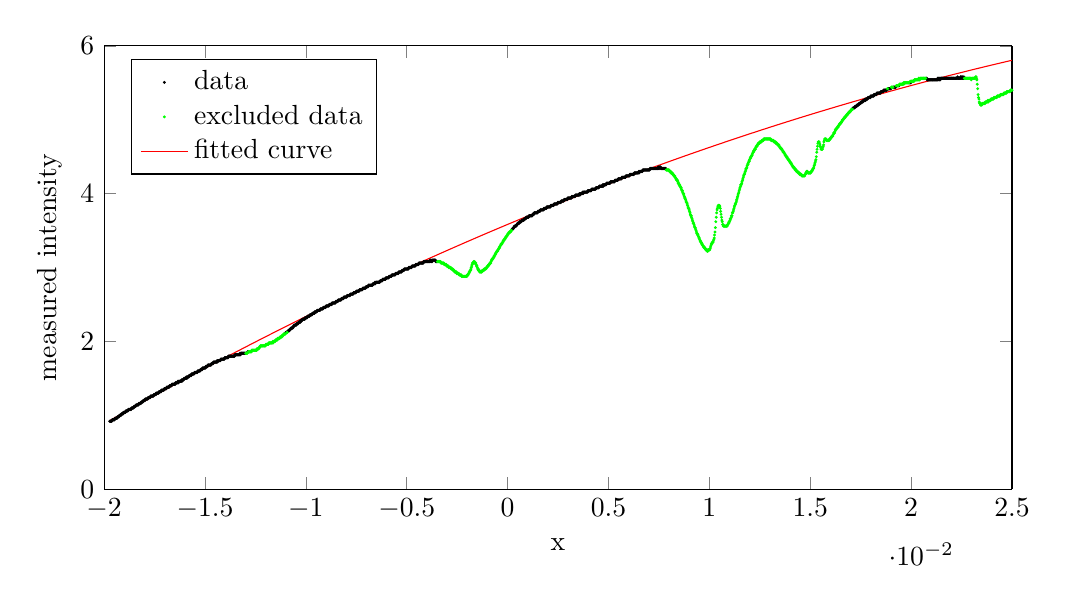
\begin{tikzpicture}

\begin{axis}[%
width=0.95092\textwidth,
height=0.464435\textwidth,
at={(0\textwidth,0\textwidth)},
scale only axis,
separate axis lines,
xmin=-0.02,
xmax=0.025,
xlabel={x},
ymin=0,
ymax=6,
ylabel={measured intensity},
legend style={at={(0.03,0.97)},anchor=north west,legend cell align=left,align=left,draw=black}
]
\addplot [color=black,only marks,mark=*,mark options={solid}, mark size=0.3]
  table[row sep=crcr]{%
-0.01972	0.92\\
-0.0197	0.92\\
-0.01968	0.92\\
-0.01966	0.92\\
-0.01964	0.92\\
-0.01962	0.92\\
-0.0196	0.94\\
-0.01958	0.94\\
-0.01956	0.94\\
-0.01954	0.94\\
-0.01952	0.94\\
-0.0195	0.94\\
-0.01948	0.94\\
-0.01946	0.96\\
-0.01944	0.96\\
-0.01942	0.96\\
-0.0194	0.96\\
-0.01938	0.96\\
-0.01936	0.96\\
-0.01934	0.98\\
-0.01932	0.98\\
-0.0193	0.98\\
-0.01928	0.98\\
-0.01926	0.98\\
-0.01924	1\\
-0.01922	1\\
-0.0192	1\\
-0.01918	1\\
-0.01916	1\\
-0.01914	1.02\\
-0.01912	1.02\\
-0.0191	1.02\\
-0.01908	1.02\\
-0.01906	1.02\\
-0.01904	1.04\\
-0.01902	1.04\\
-0.019	1.04\\
-0.01898	1.04\\
-0.01896	1.04\\
-0.01894	1.04\\
-0.01892	1.06\\
-0.0189	1.06\\
-0.01888	1.06\\
-0.01886	1.06\\
-0.01884	1.06\\
-0.01882	1.06\\
-0.0188	1.08\\
-0.01878	1.08\\
-0.01876	1.08\\
-0.01874	1.08\\
-0.01872	1.08\\
-0.0187	1.08\\
-0.01868	1.08\\
-0.01866	1.08\\
-0.01864	1.1\\
-0.01862	1.1\\
-0.0186	1.1\\
-0.01858	1.1\\
-0.01856	1.1\\
-0.01854	1.1\\
-0.01852	1.12\\
-0.0185	1.12\\
-0.01848	1.12\\
-0.01846	1.12\\
-0.01844	1.12\\
-0.01842	1.14\\
-0.0184	1.14\\
-0.01838	1.14\\
-0.01836	1.14\\
-0.01834	1.14\\
-0.01832	1.14\\
-0.0183	1.14\\
-0.01828	1.16\\
-0.01826	1.16\\
-0.01824	1.16\\
-0.01822	1.16\\
-0.0182	1.16\\
-0.01818	1.16\\
-0.01816	1.18\\
-0.01814	1.18\\
-0.01812	1.18\\
-0.0181	1.18\\
-0.01808	1.18\\
-0.01806	1.2\\
-0.01804	1.2\\
-0.01802	1.2\\
-0.018	1.2\\
-0.01798	1.2\\
-0.01796	1.22\\
-0.01794	1.22\\
-0.01792	1.22\\
-0.0179	1.22\\
-0.01788	1.22\\
-0.01786	1.22\\
-0.01784	1.22\\
-0.01782	1.24\\
-0.0178	1.24\\
-0.01778	1.24\\
-0.01776	1.24\\
-0.01774	1.24\\
-0.01772	1.24\\
-0.0177	1.26\\
-0.01768	1.26\\
-0.01766	1.26\\
-0.01764	1.26\\
-0.01762	1.26\\
-0.0176	1.26\\
-0.01758	1.26\\
-0.01756	1.26\\
-0.01754	1.28\\
-0.01752	1.28\\
-0.0175	1.28\\
-0.01748	1.28\\
-0.01746	1.28\\
-0.01744	1.28\\
-0.01742	1.3\\
-0.0174	1.3\\
-0.01738	1.3\\
-0.01736	1.3\\
-0.01734	1.3\\
-0.01732	1.3\\
-0.0173	1.3\\
-0.01728	1.32\\
-0.01726	1.32\\
-0.01724	1.32\\
-0.01722	1.32\\
-0.0172	1.32\\
-0.01718	1.32\\
-0.01716	1.34\\
-0.01714	1.34\\
-0.01712	1.34\\
-0.0171	1.34\\
-0.01708	1.34\\
-0.01706	1.34\\
-0.01704	1.34\\
-0.01702	1.36\\
-0.017	1.36\\
-0.01698	1.36\\
-0.01696	1.36\\
-0.01694	1.36\\
-0.01692	1.36\\
-0.0169	1.38\\
-0.01688	1.38\\
-0.01686	1.38\\
-0.01684	1.38\\
-0.01682	1.38\\
-0.0168	1.38\\
-0.01678	1.38\\
-0.01676	1.4\\
-0.01674	1.4\\
-0.01672	1.4\\
-0.0167	1.4\\
-0.01668	1.4\\
-0.01666	1.4\\
-0.01664	1.42\\
-0.01662	1.42\\
-0.0166	1.42\\
-0.01658	1.42\\
-0.01656	1.42\\
-0.01654	1.42\\
-0.01652	1.42\\
-0.0165	1.42\\
-0.01648	1.42\\
-0.01646	1.44\\
-0.01644	1.44\\
-0.01642	1.44\\
-0.0164	1.44\\
-0.01638	1.44\\
-0.01636	1.44\\
-0.01634	1.46\\
-0.01632	1.44\\
-0.0163	1.46\\
-0.01628	1.46\\
-0.01626	1.46\\
-0.01624	1.46\\
-0.01622	1.46\\
-0.0162	1.46\\
-0.01618	1.46\\
-0.01616	1.48\\
-0.01614	1.46\\
-0.01612	1.48\\
-0.0161	1.48\\
-0.01608	1.48\\
-0.01606	1.48\\
-0.01604	1.5\\
-0.01602	1.5\\
-0.016	1.5\\
-0.01598	1.5\\
-0.01596	1.5\\
-0.01594	1.5\\
-0.01592	1.52\\
-0.0159	1.5\\
-0.01588	1.52\\
-0.01586	1.52\\
-0.01584	1.52\\
-0.01582	1.52\\
-0.0158	1.52\\
-0.01578	1.54\\
-0.01576	1.54\\
-0.01574	1.54\\
-0.01572	1.54\\
-0.0157	1.54\\
-0.01568	1.54\\
-0.01566	1.56\\
-0.01564	1.56\\
-0.01562	1.56\\
-0.0156	1.56\\
-0.01558	1.56\\
-0.01556	1.56\\
-0.01554	1.56\\
-0.01552	1.58\\
-0.0155	1.58\\
-0.01548	1.58\\
-0.01546	1.58\\
-0.01544	1.58\\
-0.01542	1.58\\
-0.0154	1.58\\
-0.01538	1.58\\
-0.01536	1.6\\
-0.01534	1.6\\
-0.01532	1.6\\
-0.0153	1.6\\
-0.01528	1.6\\
-0.01526	1.6\\
-0.01524	1.6\\
-0.01522	1.62\\
-0.0152	1.62\\
-0.01518	1.62\\
-0.01516	1.62\\
-0.01514	1.62\\
-0.01512	1.64\\
-0.0151	1.64\\
-0.01508	1.64\\
-0.01506	1.64\\
-0.01504	1.64\\
-0.01502	1.64\\
-0.015	1.64\\
-0.01498	1.64\\
-0.01496	1.66\\
-0.01494	1.66\\
-0.01492	1.66\\
-0.0149	1.66\\
-0.01488	1.66\\
-0.01486	1.68\\
-0.01484	1.68\\
-0.01482	1.68\\
-0.0148	1.68\\
-0.01478	1.68\\
-0.01476	1.68\\
-0.01474	1.68\\
-0.01472	1.68\\
-0.0147	1.68\\
-0.01468	1.7\\
-0.01466	1.7\\
-0.01464	1.7\\
-0.01462	1.7\\
-0.0146	1.7\\
-0.01458	1.72\\
-0.01456	1.72\\
-0.01454	1.72\\
-0.01452	1.72\\
-0.0145	1.72\\
-0.01448	1.72\\
-0.01446	1.72\\
-0.01444	1.72\\
-0.01442	1.72\\
-0.0144	1.74\\
-0.01438	1.72\\
-0.01436	1.74\\
-0.01434	1.74\\
-0.01432	1.74\\
-0.0143	1.74\\
-0.01428	1.74\\
-0.01426	1.74\\
-0.01424	1.74\\
-0.01422	1.76\\
-0.0142	1.76\\
-0.01418	1.76\\
-0.01416	1.76\\
-0.01414	1.76\\
-0.01412	1.76\\
-0.0141	1.76\\
-0.01408	1.76\\
-0.01406	1.76\\
-0.01404	1.76\\
-0.01402	1.78\\
-0.014	1.78\\
-0.01398	1.78\\
-0.01396	1.78\\
-0.01394	1.78\\
-0.01392	1.78\\
-0.0139	1.78\\
-0.01388	1.78\\
-0.01386	1.78\\
-0.01384	1.8\\
-0.01382	1.8\\
-0.0138	1.8\\
-0.01378	1.8\\
-0.01376	1.8\\
-0.01374	1.8\\
-0.01372	1.8\\
-0.0137	1.8\\
-0.01368	1.8\\
-0.01366	1.8\\
-0.01364	1.8\\
-0.01362	1.8\\
-0.0136	1.8\\
-0.01358	1.8\\
-0.01356	1.8\\
-0.01354	1.8\\
-0.01352	1.82\\
-0.0135	1.82\\
-0.01348	1.82\\
-0.01346	1.82\\
-0.01344	1.82\\
-0.01342	1.82\\
-0.0134	1.82\\
-0.01338	1.82\\
-0.01336	1.82\\
-0.01334	1.82\\
-0.01332	1.82\\
-0.0133	1.82\\
-0.01328	1.82\\
-0.01326	1.84\\
-0.01324	1.82\\
-0.01322	1.84\\
-0.0132	1.84\\
-0.01318	1.84\\
-0.01316	1.84\\
-0.01314	1.84\\
-0.01312	1.84\\
-0.0131	1.84\\
-0.01308	1.84\\
-0.01306	1.84\\
-0.01304	1.84\\
-0.01302	1.84\\
-0.013	1.84\\
-0.01288	1.86\\
-0.01286	1.86\\
-0.011	2.12\\
-0.01098	2.12\\
-0.01096	2.12\\
-0.0109	2.14\\
-0.01088	2.14\\
-0.01086	2.14\\
-0.01084	2.14\\
-0.01082	2.16\\
-0.0108	2.16\\
-0.01078	2.16\\
-0.01076	2.16\\
-0.01074	2.18\\
-0.01072	2.18\\
-0.0107	2.18\\
-0.01068	2.18\\
-0.01066	2.18\\
-0.01064	2.2\\
-0.01062	2.2\\
-0.0106	2.2\\
-0.01058	2.22\\
-0.01056	2.22\\
-0.01054	2.22\\
-0.01052	2.22\\
-0.0105	2.22\\
-0.01048	2.22\\
-0.01046	2.24\\
-0.01044	2.24\\
-0.01042	2.24\\
-0.0104	2.24\\
-0.01038	2.24\\
-0.01036	2.26\\
-0.01034	2.26\\
-0.01032	2.26\\
-0.0103	2.26\\
-0.01028	2.26\\
-0.01026	2.28\\
-0.01024	2.28\\
-0.01022	2.28\\
-0.0102	2.28\\
-0.01018	2.3\\
-0.01016	2.3\\
-0.01014	2.3\\
-0.01012	2.3\\
-0.0101	2.3\\
-0.01008	2.3\\
-0.01006	2.3\\
-0.01004	2.32\\
-0.01002	2.32\\
-0.01	2.32\\
-0.00998	2.32\\
-0.00996	2.32\\
-0.00994	2.32\\
-0.00992	2.34\\
-0.0099	2.34\\
-0.00988	2.34\\
-0.00986	2.34\\
-0.00984	2.34\\
-0.00982	2.34\\
-0.0098	2.36\\
-0.00978	2.36\\
-0.00976	2.36\\
-0.00974	2.36\\
-0.00972	2.36\\
-0.0097	2.36\\
-0.00968	2.38\\
-0.00966	2.38\\
-0.00964	2.38\\
-0.00962	2.38\\
-0.0096	2.38\\
-0.00958	2.38\\
-0.00956	2.4\\
-0.00954	2.4\\
-0.00952	2.4\\
-0.0095	2.4\\
-0.00948	2.4\\
-0.00946	2.4\\
-0.00944	2.42\\
-0.00942	2.42\\
-0.0094	2.42\\
-0.00938	2.42\\
-0.00936	2.42\\
-0.00934	2.42\\
-0.00932	2.42\\
-0.0093	2.42\\
-0.00928	2.44\\
-0.00926	2.44\\
-0.00924	2.44\\
-0.00922	2.44\\
-0.0092	2.44\\
-0.00918	2.44\\
-0.00916	2.44\\
-0.00914	2.46\\
-0.00912	2.46\\
-0.0091	2.46\\
-0.00908	2.46\\
-0.00906	2.46\\
-0.00904	2.46\\
-0.00902	2.46\\
-0.009	2.48\\
-0.00898	2.48\\
-0.00896	2.48\\
-0.00894	2.48\\
-0.00892	2.48\\
-0.0089	2.48\\
-0.00888	2.48\\
-0.00886	2.48\\
-0.00884	2.5\\
-0.00882	2.5\\
-0.0088	2.5\\
-0.00878	2.5\\
-0.00876	2.5\\
-0.00874	2.5\\
-0.00872	2.5\\
-0.0087	2.52\\
-0.00868	2.52\\
-0.00866	2.52\\
-0.00864	2.52\\
-0.00862	2.52\\
-0.0086	2.52\\
-0.00858	2.52\\
-0.00856	2.52\\
-0.00854	2.52\\
-0.00852	2.54\\
-0.0085	2.54\\
-0.00848	2.54\\
-0.00846	2.54\\
-0.00844	2.54\\
-0.00842	2.54\\
-0.0084	2.56\\
-0.00838	2.56\\
-0.00836	2.56\\
-0.00834	2.56\\
-0.00832	2.56\\
-0.0083	2.56\\
-0.00828	2.56\\
-0.00826	2.56\\
-0.00824	2.58\\
-0.00822	2.58\\
-0.0082	2.58\\
-0.00818	2.58\\
-0.00816	2.58\\
-0.00814	2.58\\
-0.00812	2.6\\
-0.0081	2.6\\
-0.00808	2.6\\
-0.00806	2.6\\
-0.00804	2.6\\
-0.00802	2.6\\
-0.008	2.6\\
-0.00798	2.6\\
-0.00796	2.62\\
-0.00794	2.62\\
-0.00792	2.62\\
-0.0079	2.62\\
-0.00788	2.62\\
-0.00786	2.62\\
-0.00784	2.62\\
-0.00782	2.62\\
-0.0078	2.64\\
-0.00778	2.64\\
-0.00776	2.64\\
-0.00774	2.64\\
-0.00772	2.64\\
-0.0077	2.64\\
-0.00768	2.64\\
-0.00766	2.64\\
-0.00764	2.66\\
-0.00762	2.66\\
-0.0076	2.66\\
-0.00758	2.66\\
-0.00756	2.66\\
-0.00754	2.66\\
-0.00752	2.66\\
-0.0075	2.68\\
-0.00748	2.68\\
-0.00746	2.68\\
-0.00744	2.68\\
-0.00742	2.68\\
-0.0074	2.68\\
-0.00738	2.68\\
-0.00736	2.68\\
-0.00734	2.7\\
-0.00732	2.7\\
-0.0073	2.7\\
-0.00728	2.7\\
-0.00726	2.7\\
-0.00724	2.7\\
-0.00722	2.7\\
-0.0072	2.7\\
-0.00718	2.72\\
-0.00716	2.72\\
-0.00714	2.72\\
-0.00712	2.72\\
-0.0071	2.72\\
-0.00708	2.72\\
-0.00706	2.72\\
-0.00704	2.72\\
-0.00702	2.74\\
-0.007	2.74\\
-0.00698	2.74\\
-0.00696	2.74\\
-0.00694	2.74\\
-0.00692	2.74\\
-0.0069	2.76\\
-0.00688	2.76\\
-0.00686	2.76\\
-0.00684	2.76\\
-0.00682	2.76\\
-0.0068	2.76\\
-0.00678	2.76\\
-0.00676	2.76\\
-0.00674	2.76\\
-0.00672	2.76\\
-0.0067	2.76\\
-0.00668	2.78\\
-0.00666	2.78\\
-0.00664	2.78\\
-0.00662	2.78\\
-0.0066	2.78\\
-0.00658	2.8\\
-0.00656	2.78\\
-0.00654	2.8\\
-0.00652	2.8\\
-0.0065	2.8\\
-0.00648	2.8\\
-0.00646	2.8\\
-0.00644	2.8\\
-0.00642	2.8\\
-0.0064	2.8\\
-0.00638	2.8\\
-0.00636	2.8\\
-0.00634	2.8\\
-0.00632	2.82\\
-0.0063	2.82\\
-0.00628	2.82\\
-0.00626	2.82\\
-0.00624	2.82\\
-0.00622	2.82\\
-0.0062	2.84\\
-0.00618	2.84\\
-0.00616	2.84\\
-0.00614	2.84\\
-0.00612	2.84\\
-0.0061	2.84\\
-0.00608	2.84\\
-0.00606	2.84\\
-0.00604	2.86\\
-0.00602	2.86\\
-0.006	2.86\\
-0.00598	2.86\\
-0.00596	2.86\\
-0.00594	2.86\\
-0.00592	2.86\\
-0.0059	2.86\\
-0.00588	2.88\\
-0.00586	2.88\\
-0.00584	2.88\\
-0.00582	2.88\\
-0.0058	2.88\\
-0.00578	2.88\\
-0.00576	2.88\\
-0.00574	2.9\\
-0.00572	2.9\\
-0.0057	2.9\\
-0.00568	2.9\\
-0.00566	2.9\\
-0.00564	2.9\\
-0.00562	2.9\\
-0.0056	2.9\\
-0.00558	2.9\\
-0.00556	2.92\\
-0.00554	2.92\\
-0.00552	2.92\\
-0.0055	2.92\\
-0.00548	2.92\\
-0.00546	2.92\\
-0.00544	2.92\\
-0.00542	2.92\\
-0.0054	2.94\\
-0.00538	2.94\\
-0.00536	2.94\\
-0.00534	2.94\\
-0.00532	2.94\\
-0.0053	2.94\\
-0.00528	2.94\\
-0.00526	2.94\\
-0.00524	2.96\\
-0.00522	2.96\\
-0.0052	2.96\\
-0.00518	2.96\\
-0.00516	2.96\\
-0.00514	2.96\\
-0.00512	2.98\\
-0.0051	2.98\\
-0.00508	2.98\\
-0.00506	2.98\\
-0.00504	2.98\\
-0.00502	2.98\\
-0.005	2.98\\
-0.00498	2.98\\
-0.00496	2.98\\
-0.00494	2.98\\
-0.00492	2.98\\
-0.0049	3\\
-0.00488	3\\
-0.00486	3\\
-0.00484	3\\
-0.00482	3\\
-0.0048	3\\
-0.00478	3\\
-0.00476	3\\
-0.00474	3.02\\
-0.00472	3.02\\
-0.0047	3.02\\
-0.00468	3.02\\
-0.00466	3.02\\
-0.00464	3.02\\
-0.00462	3.02\\
-0.0046	3.02\\
-0.00458	3.02\\
-0.00456	3.04\\
-0.00454	3.04\\
-0.00452	3.04\\
-0.0045	3.04\\
-0.00448	3.04\\
-0.00446	3.04\\
-0.00444	3.04\\
-0.00442	3.04\\
-0.0044	3.06\\
-0.00438	3.06\\
-0.00436	3.06\\
-0.00434	3.06\\
-0.00432	3.06\\
-0.0043	3.06\\
-0.00428	3.06\\
-0.00426	3.06\\
-0.00424	3.06\\
-0.00422	3.06\\
-0.0042	3.06\\
-0.00418	3.06\\
-0.00416	3.08\\
-0.00414	3.08\\
-0.00412	3.08\\
-0.0041	3.08\\
-0.00408	3.08\\
-0.00406	3.08\\
-0.00404	3.08\\
-0.00402	3.08\\
-0.004	3.08\\
-0.00398	3.08\\
-0.00396	3.08\\
-0.00394	3.08\\
-0.00392	3.08\\
-0.0039	3.08\\
-0.00388	3.08\\
-0.00386	3.08\\
-0.00384	3.1\\
-0.00382	3.1\\
-0.0038	3.08\\
-0.00378	3.08\\
-0.00376	3.1\\
-0.00374	3.08\\
-0.00372	3.1\\
-0.0037	3.1\\
-0.00368	3.1\\
-0.00366	3.1\\
-0.00364	3.1\\
-0.00362	3.1\\
-0.0036	3.1\\
-0.00358	3.1\\
-0.00356	3.08\\
-0.00354	3.08\\
-0.00352	3.08\\
-0.0035	3.08\\
0.00022	3.52\\
0.00024	3.52\\
0.00026	3.52\\
0.00028	3.54\\
0.0003	3.54\\
0.00032	3.54\\
0.00034	3.56\\
0.00036	3.56\\
0.00038	3.56\\
0.0004	3.56\\
0.00042	3.56\\
0.00044	3.58\\
0.00046	3.58\\
0.00048	3.58\\
0.0005	3.6\\
0.00052	3.6\\
0.00054	3.6\\
0.00056	3.6\\
0.00058	3.6\\
0.0006	3.62\\
0.00062	3.62\\
0.00064	3.62\\
0.00066	3.62\\
0.00068	3.62\\
0.0007	3.64\\
0.00072	3.64\\
0.00074	3.64\\
0.00076	3.64\\
0.00078	3.64\\
0.0008	3.64\\
0.00082	3.66\\
0.00084	3.66\\
0.00086	3.66\\
0.00088	3.66\\
0.0009	3.66\\
0.00092	3.68\\
0.00094	3.68\\
0.00096	3.68\\
0.00098	3.68\\
0.001	3.68\\
0.00102	3.68\\
0.00104	3.68\\
0.00106	3.7\\
0.00108	3.7\\
0.0011	3.7\\
0.00112	3.7\\
0.00114	3.7\\
0.00116	3.7\\
0.00118	3.7\\
0.0012	3.7\\
0.00122	3.7\\
0.00124	3.72\\
0.00126	3.72\\
0.00128	3.72\\
0.0013	3.72\\
0.00132	3.74\\
0.00134	3.74\\
0.00136	3.74\\
0.00138	3.74\\
0.0014	3.74\\
0.00142	3.74\\
0.00144	3.74\\
0.00146	3.74\\
0.00148	3.74\\
0.0015	3.76\\
0.00152	3.76\\
0.00154	3.76\\
0.00156	3.76\\
0.00158	3.76\\
0.0016	3.76\\
0.00162	3.78\\
0.00164	3.78\\
0.00166	3.78\\
0.00168	3.78\\
0.0017	3.78\\
0.00172	3.78\\
0.00174	3.78\\
0.00176	3.78\\
0.00178	3.78\\
0.0018	3.8\\
0.00182	3.8\\
0.00184	3.8\\
0.00186	3.8\\
0.00188	3.8\\
0.0019	3.8\\
0.00192	3.8\\
0.00194	3.82\\
0.00196	3.82\\
0.00198	3.82\\
0.002	3.82\\
0.00202	3.82\\
0.00204	3.82\\
0.00206	3.82\\
0.00208	3.82\\
0.0021	3.82\\
0.00212	3.82\\
0.00214	3.84\\
0.00216	3.84\\
0.00218	3.84\\
0.0022	3.84\\
0.00222	3.84\\
0.00224	3.84\\
0.00226	3.84\\
0.00228	3.84\\
0.0023	3.86\\
0.00232	3.86\\
0.00234	3.86\\
0.00236	3.86\\
0.00238	3.86\\
0.0024	3.86\\
0.00242	3.86\\
0.00244	3.86\\
0.00246	3.86\\
0.00248	3.88\\
0.0025	3.88\\
0.00252	3.88\\
0.00254	3.88\\
0.00256	3.88\\
0.00258	3.88\\
0.0026	3.88\\
0.00262	3.88\\
0.00264	3.88\\
0.00266	3.9\\
0.00268	3.9\\
0.0027	3.9\\
0.00272	3.9\\
0.00274	3.9\\
0.00276	3.9\\
0.00278	3.9\\
0.0028	3.92\\
0.00282	3.92\\
0.00284	3.92\\
0.00286	3.92\\
0.00288	3.92\\
0.0029	3.92\\
0.00292	3.92\\
0.00294	3.92\\
0.00296	3.92\\
0.00298	3.94\\
0.003	3.94\\
0.00302	3.94\\
0.00304	3.94\\
0.00306	3.94\\
0.00308	3.94\\
0.0031	3.94\\
0.00312	3.94\\
0.00314	3.94\\
0.00316	3.94\\
0.00318	3.96\\
0.0032	3.96\\
0.00322	3.96\\
0.00324	3.96\\
0.00326	3.96\\
0.00328	3.96\\
0.0033	3.96\\
0.00332	3.96\\
0.00334	3.96\\
0.00336	3.98\\
0.00338	3.98\\
0.0034	3.98\\
0.00342	3.98\\
0.00344	3.98\\
0.00346	3.98\\
0.00348	3.98\\
0.0035	3.98\\
0.00352	3.98\\
0.00354	3.98\\
0.00356	4\\
0.00358	3.98\\
0.0036	4\\
0.00362	4\\
0.00364	4\\
0.00366	4\\
0.00368	4\\
0.0037	4\\
0.00372	4.02\\
0.00374	4\\
0.00376	4.02\\
0.00378	4.02\\
0.0038	4.02\\
0.00382	4.02\\
0.00384	4.02\\
0.00386	4.02\\
0.00388	4.02\\
0.0039	4.02\\
0.00392	4.02\\
0.00394	4.02\\
0.00396	4.02\\
0.00398	4.04\\
0.004	4.04\\
0.00402	4.04\\
0.00404	4.04\\
0.00406	4.04\\
0.00408	4.04\\
0.0041	4.04\\
0.00412	4.04\\
0.00414	4.04\\
0.00416	4.06\\
0.00418	4.06\\
0.0042	4.06\\
0.00422	4.06\\
0.00424	4.06\\
0.00426	4.06\\
0.00428	4.06\\
0.0043	4.06\\
0.00432	4.06\\
0.00434	4.06\\
0.00436	4.06\\
0.00438	4.08\\
0.0044	4.08\\
0.00442	4.08\\
0.00444	4.08\\
0.00446	4.08\\
0.00448	4.08\\
0.0045	4.08\\
0.00452	4.08\\
0.00454	4.1\\
0.00456	4.1\\
0.00458	4.1\\
0.0046	4.1\\
0.00462	4.1\\
0.00464	4.1\\
0.00466	4.1\\
0.00468	4.1\\
0.0047	4.1\\
0.00472	4.12\\
0.00474	4.1\\
0.00476	4.12\\
0.00478	4.12\\
0.0048	4.12\\
0.00482	4.12\\
0.00484	4.12\\
0.00486	4.12\\
0.00488	4.12\\
0.0049	4.14\\
0.00492	4.14\\
0.00494	4.14\\
0.00496	4.14\\
0.00498	4.14\\
0.005	4.14\\
0.00502	4.14\\
0.00504	4.14\\
0.00506	4.14\\
0.00508	4.14\\
0.0051	4.16\\
0.00512	4.16\\
0.00514	4.16\\
0.00516	4.16\\
0.00518	4.16\\
0.0052	4.16\\
0.00522	4.16\\
0.00524	4.16\\
0.00526	4.16\\
0.00528	4.16\\
0.0053	4.16\\
0.00532	4.18\\
0.00534	4.18\\
0.00536	4.18\\
0.00538	4.18\\
0.0054	4.18\\
0.00542	4.18\\
0.00544	4.18\\
0.00546	4.18\\
0.00548	4.2\\
0.0055	4.2\\
0.00552	4.2\\
0.00554	4.2\\
0.00556	4.2\\
0.00558	4.2\\
0.0056	4.2\\
0.00562	4.2\\
0.00564	4.2\\
0.00566	4.22\\
0.00568	4.22\\
0.0057	4.22\\
0.00572	4.22\\
0.00574	4.22\\
0.00576	4.22\\
0.00578	4.22\\
0.0058	4.22\\
0.00582	4.22\\
0.00584	4.22\\
0.00586	4.24\\
0.00588	4.24\\
0.0059	4.24\\
0.00592	4.24\\
0.00594	4.24\\
0.00596	4.24\\
0.00598	4.24\\
0.006	4.24\\
0.00602	4.24\\
0.00604	4.24\\
0.00606	4.26\\
0.00608	4.26\\
0.0061	4.26\\
0.00612	4.26\\
0.00614	4.26\\
0.00616	4.26\\
0.00618	4.26\\
0.0062	4.26\\
0.00622	4.26\\
0.00624	4.26\\
0.00626	4.26\\
0.00628	4.28\\
0.0063	4.28\\
0.00632	4.28\\
0.00634	4.28\\
0.00636	4.28\\
0.00638	4.28\\
0.0064	4.28\\
0.00642	4.28\\
0.00644	4.28\\
0.00646	4.28\\
0.00648	4.28\\
0.0065	4.3\\
0.00652	4.28\\
0.00654	4.3\\
0.00656	4.3\\
0.00658	4.3\\
0.0066	4.3\\
0.00662	4.3\\
0.00664	4.3\\
0.00666	4.3\\
0.00668	4.3\\
0.0067	4.32\\
0.00672	4.32\\
0.00674	4.32\\
0.00676	4.32\\
0.00678	4.32\\
0.0068	4.32\\
0.00682	4.32\\
0.00684	4.32\\
0.00686	4.32\\
0.00688	4.32\\
0.0069	4.32\\
0.00692	4.32\\
0.00694	4.32\\
0.00696	4.32\\
0.00698	4.32\\
0.007	4.32\\
0.00702	4.32\\
0.00704	4.32\\
0.00706	4.34\\
0.00708	4.34\\
0.0071	4.34\\
0.00712	4.34\\
0.00714	4.34\\
0.00716	4.34\\
0.00718	4.34\\
0.0072	4.34\\
0.00722	4.34\\
0.00724	4.34\\
0.00726	4.34\\
0.00728	4.34\\
0.0073	4.34\\
0.00732	4.34\\
0.00734	4.34\\
0.00736	4.34\\
0.00738	4.34\\
0.0074	4.34\\
0.00742	4.34\\
0.00744	4.34\\
0.00746	4.36\\
0.00748	4.34\\
0.0075	4.36\\
0.00752	4.36\\
0.00754	4.34\\
0.00756	4.36\\
0.00758	4.36\\
0.0076	4.34\\
0.00762	4.34\\
0.00764	4.34\\
0.00766	4.34\\
0.00768	4.34\\
0.0077	4.34\\
0.00772	4.34\\
0.00774	4.34\\
0.00776	4.34\\
0.00778	4.34\\
0.0078	4.34\\
0.00782	4.34\\
0.00784	4.34\\
0.01712	5.16\\
0.01714	5.16\\
0.01716	5.16\\
0.01718	5.16\\
0.0172	5.16\\
0.01722	5.18\\
0.01724	5.18\\
0.01726	5.18\\
0.01728	5.18\\
0.0173	5.18\\
0.01732	5.2\\
0.01734	5.2\\
0.01736	5.2\\
0.01738	5.2\\
0.0174	5.2\\
0.01742	5.22\\
0.01744	5.22\\
0.01746	5.22\\
0.01748	5.22\\
0.0175	5.22\\
0.01752	5.24\\
0.01754	5.24\\
0.01756	5.24\\
0.01758	5.24\\
0.0176	5.24\\
0.01762	5.26\\
0.01764	5.26\\
0.01766	5.26\\
0.01768	5.26\\
0.0177	5.26\\
0.01772	5.28\\
0.01774	5.26\\
0.01776	5.28\\
0.01778	5.28\\
0.0178	5.28\\
0.01782	5.28\\
0.01784	5.28\\
0.01786	5.3\\
0.01788	5.3\\
0.0179	5.3\\
0.01792	5.3\\
0.01794	5.3\\
0.01796	5.3\\
0.01798	5.3\\
0.018	5.32\\
0.01802	5.32\\
0.01804	5.32\\
0.01806	5.32\\
0.01808	5.32\\
0.0181	5.32\\
0.01812	5.32\\
0.01814	5.32\\
0.01816	5.34\\
0.01818	5.34\\
0.0182	5.34\\
0.01822	5.34\\
0.01824	5.34\\
0.01826	5.34\\
0.01828	5.34\\
0.0183	5.36\\
0.01832	5.36\\
0.01834	5.36\\
0.01836	5.36\\
0.01838	5.36\\
0.0184	5.36\\
0.01842	5.36\\
0.01844	5.36\\
0.01846	5.36\\
0.01848	5.36\\
0.0185	5.38\\
0.01852	5.38\\
0.01854	5.38\\
0.01856	5.38\\
0.01858	5.38\\
0.0186	5.38\\
0.01862	5.38\\
0.01864	5.4\\
0.01866	5.4\\
0.01868	5.4\\
0.0187	5.4\\
0.01872	5.4\\
0.01874	5.4\\
0.01876	5.4\\
0.01878	5.4\\
0.0188	5.4\\
0.01886	5.42\\
0.01888	5.42\\
0.0189	5.42\\
0.01892	5.42\\
0.01894	5.42\\
0.01896	5.42\\
0.01898	5.42\\
0.019	5.42\\
0.01912	5.44\\
0.01914	5.44\\
0.01916	5.44\\
0.01918	5.44\\
0.0192	5.44\\
0.01922	5.44\\
0.01924	5.44\\
0.01938	5.46\\
0.0194	5.46\\
0.01992	5.5\\
0.01994	5.5\\
0.01998	5.5\\
0.02074	5.56\\
0.02076	5.56\\
0.02078	5.56\\
0.0208	5.54\\
0.02082	5.54\\
0.02084	5.54\\
0.02086	5.54\\
0.02088	5.54\\
0.0209	5.54\\
0.02092	5.54\\
0.02094	5.54\\
0.02096	5.54\\
0.02098	5.54\\
0.021	5.54\\
0.02102	5.54\\
0.02104	5.54\\
0.02106	5.54\\
0.02108	5.54\\
0.0211	5.54\\
0.02112	5.54\\
0.02114	5.54\\
0.02116	5.54\\
0.02118	5.54\\
0.0212	5.54\\
0.02122	5.54\\
0.02124	5.54\\
0.02126	5.54\\
0.02128	5.54\\
0.0213	5.54\\
0.02132	5.56\\
0.02134	5.54\\
0.02136	5.56\\
0.02138	5.56\\
0.0214	5.54\\
0.02142	5.56\\
0.02144	5.54\\
0.02146	5.56\\
0.02148	5.56\\
0.0215	5.56\\
0.02152	5.56\\
0.02154	5.56\\
0.02156	5.56\\
0.02158	5.56\\
0.0216	5.56\\
0.02162	5.56\\
0.02164	5.56\\
0.02166	5.56\\
0.02168	5.56\\
0.0217	5.56\\
0.02172	5.56\\
0.02174	5.56\\
0.02176	5.56\\
0.02178	5.56\\
0.0218	5.56\\
0.02182	5.56\\
0.02184	5.56\\
0.02186	5.56\\
0.02188	5.56\\
0.0219	5.56\\
0.02192	5.56\\
0.02194	5.56\\
0.02196	5.56\\
0.02198	5.56\\
0.022	5.56\\
0.02202	5.56\\
0.02204	5.56\\
0.02206	5.56\\
0.02208	5.56\\
0.0221	5.56\\
0.02212	5.56\\
0.02214	5.56\\
0.02216	5.56\\
0.02218	5.56\\
0.0222	5.56\\
0.02222	5.56\\
0.02224	5.56\\
0.02226	5.56\\
0.02228	5.56\\
0.0223	5.58\\
0.02232	5.56\\
0.02234	5.56\\
0.02236	5.56\\
0.02238	5.56\\
0.0224	5.56\\
0.02242	5.56\\
0.02244	5.56\\
0.02246	5.58\\
0.02248	5.58\\
0.0225	5.56\\
0.02252	5.56\\
0.02254	5.58\\
0.02256	5.56\\
0.02258	5.56\\
0.0226	5.56\\
0.02262	5.58\\
};
\addlegendentry{data};

\addplot [color=green,only marks,mark=*,mark options={solid}, mark size=0.3]
  table[row sep=crcr]{%
-0.01298	1.84\\
-0.01296	1.84\\
-0.01294	1.84\\
-0.01292	1.84\\
-0.0129	1.84\\
-0.01284	1.86\\
-0.01282	1.86\\
-0.0128	1.86\\
-0.01278	1.86\\
-0.01276	1.86\\
-0.01274	1.86\\
-0.01272	1.86\\
-0.0127	1.86\\
-0.01268	1.88\\
-0.01266	1.88\\
-0.01264	1.88\\
-0.01262	1.88\\
-0.0126	1.88\\
-0.01258	1.88\\
-0.01256	1.88\\
-0.01254	1.88\\
-0.01252	1.88\\
-0.0125	1.88\\
-0.01248	1.88\\
-0.01246	1.88\\
-0.01244	1.88\\
-0.01242	1.9\\
-0.0124	1.9\\
-0.01238	1.9\\
-0.01236	1.9\\
-0.01234	1.9\\
-0.01232	1.92\\
-0.0123	1.92\\
-0.01228	1.92\\
-0.01226	1.94\\
-0.01224	1.94\\
-0.01222	1.94\\
-0.0122	1.94\\
-0.01218	1.94\\
-0.01216	1.94\\
-0.01214	1.94\\
-0.01212	1.94\\
-0.0121	1.94\\
-0.01208	1.94\\
-0.01206	1.94\\
-0.01204	1.94\\
-0.01202	1.94\\
-0.012	1.94\\
-0.01198	1.96\\
-0.01196	1.96\\
-0.01194	1.96\\
-0.01192	1.96\\
-0.0119	1.96\\
-0.01188	1.96\\
-0.01186	1.96\\
-0.01184	1.98\\
-0.01182	1.98\\
-0.0118	1.98\\
-0.01178	1.98\\
-0.01176	1.98\\
-0.01174	1.98\\
-0.01172	1.98\\
-0.0117	1.98\\
-0.01168	1.98\\
-0.01166	1.98\\
-0.01164	2\\
-0.01162	1.98\\
-0.0116	2\\
-0.01158	2\\
-0.01156	2\\
-0.01154	2\\
-0.01152	2\\
-0.0115	2.02\\
-0.01148	2.02\\
-0.01146	2.02\\
-0.01144	2.02\\
-0.01142	2.02\\
-0.0114	2.04\\
-0.01138	2.04\\
-0.01136	2.04\\
-0.01134	2.04\\
-0.01132	2.04\\
-0.0113	2.04\\
-0.01128	2.06\\
-0.01126	2.06\\
-0.01124	2.06\\
-0.01122	2.06\\
-0.0112	2.06\\
-0.01118	2.08\\
-0.01116	2.08\\
-0.01114	2.08\\
-0.01112	2.08\\
-0.0111	2.1\\
-0.01108	2.1\\
-0.01106	2.1\\
-0.01104	2.1\\
-0.01102	2.1\\
-0.01094	2.12\\
-0.01092	2.12\\
-0.00348	3.08\\
-0.00346	3.08\\
-0.00344	3.08\\
-0.00342	3.08\\
-0.0034	3.08\\
-0.00338	3.08\\
-0.00336	3.08\\
-0.00334	3.08\\
-0.00332	3.08\\
-0.0033	3.06\\
-0.00328	3.06\\
-0.00326	3.06\\
-0.00324	3.06\\
-0.00322	3.06\\
-0.0032	3.06\\
-0.00318	3.06\\
-0.00316	3.06\\
-0.00314	3.04\\
-0.00312	3.04\\
-0.0031	3.04\\
-0.00308	3.04\\
-0.00306	3.04\\
-0.00304	3.04\\
-0.00302	3.02\\
-0.003	3.02\\
-0.00298	3.02\\
-0.00296	3.02\\
-0.00294	3.02\\
-0.00292	3\\
-0.0029	3\\
-0.00288	3\\
-0.00286	3\\
-0.00284	3\\
-0.00282	3\\
-0.0028	2.98\\
-0.00278	2.98\\
-0.00276	2.98\\
-0.00274	2.98\\
-0.00272	2.98\\
-0.0027	2.96\\
-0.00268	2.96\\
-0.00266	2.96\\
-0.00264	2.96\\
-0.00262	2.94\\
-0.0026	2.94\\
-0.00258	2.94\\
-0.00256	2.94\\
-0.00254	2.94\\
-0.00252	2.92\\
-0.0025	2.92\\
-0.00248	2.92\\
-0.00246	2.92\\
-0.00244	2.92\\
-0.00242	2.92\\
-0.0024	2.9\\
-0.00238	2.9\\
-0.00236	2.9\\
-0.00234	2.9\\
-0.00232	2.9\\
-0.0023	2.9\\
-0.00228	2.88\\
-0.00226	2.88\\
-0.00224	2.88\\
-0.00222	2.88\\
-0.0022	2.88\\
-0.00218	2.88\\
-0.00216	2.88\\
-0.00214	2.88\\
-0.00212	2.88\\
-0.0021	2.88\\
-0.00208	2.88\\
-0.00206	2.88\\
-0.00204	2.88\\
-0.00202	2.88\\
-0.002	2.9\\
-0.00198	2.9\\
-0.00196	2.9\\
-0.00194	2.92\\
-0.00192	2.92\\
-0.0019	2.94\\
-0.00188	2.94\\
-0.00186	2.96\\
-0.00184	2.96\\
-0.00182	2.98\\
-0.0018	3\\
-0.00178	3.02\\
-0.00176	3.04\\
-0.00174	3.06\\
-0.00172	3.06\\
-0.0017	3.06\\
-0.00168	3.08\\
-0.00166	3.06\\
-0.00164	3.08\\
-0.00162	3.06\\
-0.0016	3.06\\
-0.00158	3.06\\
-0.00156	3.04\\
-0.00154	3.02\\
-0.00152	3.02\\
-0.0015	3\\
-0.00148	2.98\\
-0.00146	2.98\\
-0.00144	2.96\\
-0.00142	2.96\\
-0.0014	2.96\\
-0.00138	2.94\\
-0.00136	2.94\\
-0.00134	2.94\\
-0.00132	2.94\\
-0.0013	2.94\\
-0.00128	2.94\\
-0.00126	2.96\\
-0.00124	2.96\\
-0.00122	2.96\\
-0.0012	2.96\\
-0.00118	2.96\\
-0.00116	2.98\\
-0.00114	2.98\\
-0.00112	2.98\\
-0.0011	2.98\\
-0.00108	2.98\\
-0.00106	3\\
-0.00104	3\\
-0.00102	3\\
-0.001	3.02\\
-0.00098	3.02\\
-0.00096	3.02\\
-0.00094	3.04\\
-0.00092	3.04\\
-0.0009	3.04\\
-0.00088	3.06\\
-0.00086	3.06\\
-0.00084	3.06\\
-0.00082	3.08\\
-0.0008	3.1\\
-0.00078	3.1\\
-0.00076	3.12\\
-0.00074	3.12\\
-0.00072	3.12\\
-0.0007	3.14\\
-0.00068	3.14\\
-0.00066	3.16\\
-0.00064	3.16\\
-0.00062	3.18\\
-0.0006	3.18\\
-0.00058	3.2\\
-0.00056	3.2\\
-0.00054	3.22\\
-0.00052	3.22\\
-0.0005	3.22\\
-0.00048	3.24\\
-0.00046	3.24\\
-0.00044	3.26\\
-0.00042	3.26\\
-0.0004	3.28\\
-0.00038	3.28\\
-0.00036	3.3\\
-0.00034	3.3\\
-0.00032	3.32\\
-0.0003	3.32\\
-0.00028	3.32\\
-0.00026	3.34\\
-0.00024	3.34\\
-0.00022	3.36\\
-0.0002	3.36\\
-0.00018	3.38\\
-0.00016	3.38\\
-0.00014	3.38\\
-0.00012	3.4\\
-0.0001	3.4\\
-8e-05	3.42\\
-6e-05	3.42\\
-4e-05	3.42\\
-2e-05	3.44\\
-0	3.44\\
2e-05	3.46\\
4e-05	3.46\\
6e-05	3.46\\
8e-05	3.48\\
0.0001	3.48\\
0.00012	3.48\\
0.00014	3.48\\
0.00016	3.5\\
0.00018	3.5\\
0.0002	3.5\\
0.00786	4.32\\
0.00788	4.32\\
0.0079	4.32\\
0.00792	4.32\\
0.00794	4.32\\
0.00796	4.32\\
0.00798	4.32\\
0.008	4.32\\
0.00802	4.3\\
0.00804	4.3\\
0.00806	4.3\\
0.00808	4.3\\
0.0081	4.28\\
0.00812	4.28\\
0.00814	4.28\\
0.00816	4.28\\
0.00818	4.26\\
0.0082	4.26\\
0.00822	4.26\\
0.00824	4.24\\
0.00826	4.24\\
0.00828	4.24\\
0.0083	4.22\\
0.00832	4.22\\
0.00834	4.2\\
0.00836	4.2\\
0.00838	4.18\\
0.0084	4.18\\
0.00842	4.18\\
0.00844	4.16\\
0.00846	4.14\\
0.00848	4.14\\
0.0085	4.12\\
0.00852	4.12\\
0.00854	4.1\\
0.00856	4.1\\
0.00858	4.08\\
0.0086	4.08\\
0.00862	4.06\\
0.00864	4.04\\
0.00866	4.04\\
0.00868	4.02\\
0.0087	4\\
0.00872	4\\
0.00874	3.98\\
0.00876	3.96\\
0.00878	3.94\\
0.0088	3.94\\
0.00882	3.92\\
0.00884	3.9\\
0.00886	3.88\\
0.00888	3.88\\
0.0089	3.86\\
0.00892	3.84\\
0.00894	3.82\\
0.00896	3.8\\
0.00898	3.8\\
0.009	3.78\\
0.00902	3.76\\
0.00904	3.74\\
0.00906	3.72\\
0.00908	3.7\\
0.0091	3.7\\
0.00912	3.68\\
0.00914	3.66\\
0.00916	3.64\\
0.00918	3.62\\
0.0092	3.6\\
0.00922	3.6\\
0.00924	3.58\\
0.00926	3.56\\
0.00928	3.54\\
0.0093	3.54\\
0.00932	3.52\\
0.00934	3.5\\
0.00936	3.48\\
0.00938	3.46\\
0.0094	3.46\\
0.00942	3.44\\
0.00944	3.44\\
0.00946	3.42\\
0.00948	3.4\\
0.0095	3.4\\
0.00952	3.38\\
0.00954	3.36\\
0.00956	3.36\\
0.00958	3.34\\
0.0096	3.34\\
0.00962	3.32\\
0.00964	3.32\\
0.00966	3.3\\
0.00968	3.3\\
0.0097	3.28\\
0.00972	3.28\\
0.00974	3.28\\
0.00976	3.26\\
0.00978	3.26\\
0.0098	3.26\\
0.00982	3.24\\
0.00984	3.24\\
0.00986	3.24\\
0.00988	3.24\\
0.0099	3.22\\
0.00992	3.22\\
0.00994	3.24\\
0.00996	3.24\\
0.00998	3.24\\
0.01	3.24\\
0.01002	3.24\\
0.01004	3.26\\
0.01006	3.28\\
0.01008	3.3\\
0.0101	3.32\\
0.01012	3.32\\
0.01014	3.34\\
0.01016	3.34\\
0.01018	3.34\\
0.0102	3.36\\
0.01022	3.38\\
0.01024	3.4\\
0.01026	3.44\\
0.01028	3.48\\
0.0103	3.54\\
0.01032	3.62\\
0.01034	3.68\\
0.01036	3.74\\
0.01038	3.78\\
0.0104	3.8\\
0.01042	3.82\\
0.01044	3.84\\
0.01046	3.84\\
0.01048	3.84\\
0.0105	3.84\\
0.01052	3.82\\
0.01054	3.8\\
0.01056	3.76\\
0.01058	3.72\\
0.0106	3.68\\
0.01062	3.64\\
0.01064	3.62\\
0.01066	3.58\\
0.01068	3.58\\
0.0107	3.56\\
0.01072	3.56\\
0.01074	3.56\\
0.01076	3.56\\
0.01078	3.56\\
0.0108	3.56\\
0.01082	3.56\\
0.01084	3.56\\
0.01086	3.56\\
0.01088	3.56\\
0.0109	3.58\\
0.01092	3.58\\
0.01094	3.6\\
0.01096	3.6\\
0.01098	3.62\\
0.011	3.62\\
0.01102	3.64\\
0.01104	3.66\\
0.01106	3.66\\
0.01108	3.68\\
0.0111	3.7\\
0.01112	3.7\\
0.01114	3.74\\
0.01116	3.74\\
0.01118	3.76\\
0.0112	3.78\\
0.01122	3.8\\
0.01124	3.82\\
0.01126	3.84\\
0.01128	3.86\\
0.0113	3.86\\
0.01132	3.88\\
0.01134	3.9\\
0.01136	3.92\\
0.01138	3.94\\
0.0114	3.96\\
0.01142	3.98\\
0.01144	4\\
0.01146	4.02\\
0.01148	4.04\\
0.0115	4.06\\
0.01152	4.08\\
0.01154	4.1\\
0.01156	4.12\\
0.01158	4.12\\
0.0116	4.14\\
0.01162	4.16\\
0.01164	4.18\\
0.01166	4.2\\
0.01168	4.22\\
0.0117	4.24\\
0.01172	4.26\\
0.01174	4.26\\
0.01176	4.28\\
0.01178	4.3\\
0.0118	4.32\\
0.01182	4.34\\
0.01184	4.34\\
0.01186	4.36\\
0.01188	4.38\\
0.0119	4.4\\
0.01192	4.4\\
0.01194	4.42\\
0.01196	4.44\\
0.01198	4.44\\
0.012	4.46\\
0.01202	4.48\\
0.01204	4.48\\
0.01206	4.5\\
0.01208	4.5\\
0.0121	4.52\\
0.01212	4.52\\
0.01214	4.54\\
0.01216	4.56\\
0.01218	4.56\\
0.0122	4.58\\
0.01222	4.58\\
0.01224	4.6\\
0.01226	4.6\\
0.01228	4.6\\
0.0123	4.62\\
0.01232	4.64\\
0.01234	4.64\\
0.01236	4.64\\
0.01238	4.66\\
0.0124	4.66\\
0.01242	4.68\\
0.01244	4.68\\
0.01246	4.68\\
0.01248	4.68\\
0.0125	4.7\\
0.01252	4.7\\
0.01254	4.7\\
0.01256	4.7\\
0.01258	4.7\\
0.0126	4.72\\
0.01262	4.72\\
0.01264	4.72\\
0.01266	4.72\\
0.01268	4.72\\
0.0127	4.74\\
0.01272	4.74\\
0.01274	4.74\\
0.01276	4.74\\
0.01278	4.74\\
0.0128	4.74\\
0.01282	4.74\\
0.01284	4.74\\
0.01286	4.74\\
0.01288	4.74\\
0.0129	4.74\\
0.01292	4.74\\
0.01294	4.74\\
0.01296	4.74\\
0.01298	4.74\\
0.013	4.74\\
0.01302	4.74\\
0.01304	4.74\\
0.01306	4.72\\
0.01308	4.72\\
0.0131	4.72\\
0.01312	4.72\\
0.01314	4.72\\
0.01316	4.72\\
0.01318	4.72\\
0.0132	4.7\\
0.01322	4.7\\
0.01324	4.7\\
0.01326	4.7\\
0.01328	4.7\\
0.0133	4.68\\
0.01332	4.68\\
0.01334	4.68\\
0.01336	4.68\\
0.01338	4.66\\
0.0134	4.66\\
0.01342	4.66\\
0.01344	4.66\\
0.01346	4.64\\
0.01348	4.64\\
0.0135	4.62\\
0.01352	4.62\\
0.01354	4.62\\
0.01356	4.6\\
0.01358	4.6\\
0.0136	4.6\\
0.01362	4.58\\
0.01364	4.58\\
0.01366	4.56\\
0.01368	4.56\\
0.0137	4.56\\
0.01372	4.54\\
0.01374	4.54\\
0.01376	4.52\\
0.01378	4.52\\
0.0138	4.5\\
0.01382	4.5\\
0.01384	4.5\\
0.01386	4.48\\
0.01388	4.48\\
0.0139	4.46\\
0.01392	4.46\\
0.01394	4.46\\
0.01396	4.44\\
0.01398	4.44\\
0.014	4.42\\
0.01402	4.42\\
0.01404	4.42\\
0.01406	4.4\\
0.01408	4.4\\
0.0141	4.38\\
0.01412	4.38\\
0.01414	4.36\\
0.01416	4.36\\
0.01418	4.36\\
0.0142	4.34\\
0.01422	4.34\\
0.01424	4.34\\
0.01426	4.32\\
0.01428	4.32\\
0.0143	4.32\\
0.01432	4.3\\
0.01434	4.3\\
0.01436	4.3\\
0.01438	4.3\\
0.0144	4.28\\
0.01442	4.28\\
0.01444	4.28\\
0.01446	4.28\\
0.01448	4.26\\
0.0145	4.26\\
0.01452	4.26\\
0.01454	4.26\\
0.01456	4.26\\
0.01458	4.24\\
0.0146	4.24\\
0.01462	4.24\\
0.01464	4.24\\
0.01466	4.24\\
0.01468	4.24\\
0.0147	4.24\\
0.01472	4.24\\
0.01474	4.26\\
0.01476	4.26\\
0.01478	4.28\\
0.0148	4.28\\
0.01482	4.3\\
0.01484	4.3\\
0.01486	4.3\\
0.01488	4.28\\
0.0149	4.28\\
0.01492	4.28\\
0.01494	4.28\\
0.01496	4.28\\
0.01498	4.28\\
0.015	4.28\\
0.01502	4.28\\
0.01504	4.3\\
0.01506	4.3\\
0.01508	4.3\\
0.0151	4.32\\
0.01512	4.32\\
0.01514	4.34\\
0.01516	4.34\\
0.01518	4.36\\
0.0152	4.38\\
0.01522	4.4\\
0.01524	4.42\\
0.01526	4.44\\
0.01528	4.46\\
0.0153	4.5\\
0.01532	4.56\\
0.01534	4.6\\
0.01536	4.64\\
0.01538	4.68\\
0.0154	4.7\\
0.01542	4.7\\
0.01544	4.7\\
0.01546	4.68\\
0.01548	4.66\\
0.0155	4.64\\
0.01552	4.62\\
0.01554	4.6\\
0.01556	4.6\\
0.01558	4.6\\
0.0156	4.6\\
0.01562	4.62\\
0.01564	4.64\\
0.01566	4.66\\
0.01568	4.7\\
0.0157	4.72\\
0.01572	4.74\\
0.01574	4.74\\
0.01576	4.74\\
0.01578	4.74\\
0.0158	4.72\\
0.01582	4.72\\
0.01584	4.72\\
0.01586	4.72\\
0.01588	4.72\\
0.0159	4.72\\
0.01592	4.72\\
0.01594	4.72\\
0.01596	4.74\\
0.01598	4.74\\
0.016	4.74\\
0.01602	4.76\\
0.01604	4.76\\
0.01606	4.76\\
0.01608	4.78\\
0.0161	4.78\\
0.01612	4.78\\
0.01614	4.8\\
0.01616	4.82\\
0.01618	4.82\\
0.0162	4.82\\
0.01622	4.84\\
0.01624	4.86\\
0.01626	4.86\\
0.01628	4.88\\
0.0163	4.88\\
0.01632	4.88\\
0.01634	4.9\\
0.01636	4.9\\
0.01638	4.9\\
0.0164	4.92\\
0.01642	4.92\\
0.01644	4.94\\
0.01646	4.94\\
0.01648	4.94\\
0.0165	4.96\\
0.01652	4.96\\
0.01654	4.96\\
0.01656	4.98\\
0.01658	4.98\\
0.0166	5\\
0.01662	5\\
0.01664	5\\
0.01666	5.02\\
0.01668	5.02\\
0.0167	5.02\\
0.01672	5.04\\
0.01674	5.04\\
0.01676	5.04\\
0.01678	5.06\\
0.0168	5.06\\
0.01682	5.06\\
0.01684	5.08\\
0.01686	5.08\\
0.01688	5.08\\
0.0169	5.1\\
0.01692	5.1\\
0.01694	5.1\\
0.01696	5.1\\
0.01698	5.12\\
0.017	5.12\\
0.01702	5.12\\
0.01704	5.14\\
0.01706	5.14\\
0.01708	5.14\\
0.0171	5.14\\
0.01882	5.42\\
0.01884	5.42\\
0.01902	5.44\\
0.01904	5.44\\
0.01906	5.44\\
0.01908	5.44\\
0.0191	5.44\\
0.01926	5.46\\
0.01928	5.46\\
0.0193	5.46\\
0.01932	5.46\\
0.01934	5.46\\
0.01936	5.46\\
0.01942	5.48\\
0.01944	5.48\\
0.01946	5.48\\
0.01948	5.48\\
0.0195	5.48\\
0.01952	5.48\\
0.01954	5.48\\
0.01956	5.48\\
0.01958	5.48\\
0.0196	5.48\\
0.01962	5.5\\
0.01964	5.48\\
0.01966	5.5\\
0.01968	5.5\\
0.0197	5.5\\
0.01972	5.5\\
0.01974	5.5\\
0.01976	5.5\\
0.01978	5.5\\
0.0198	5.5\\
0.01982	5.5\\
0.01984	5.5\\
0.01986	5.5\\
0.01988	5.5\\
0.0199	5.5\\
0.01996	5.52\\
0.02	5.52\\
0.02002	5.52\\
0.02004	5.52\\
0.02006	5.52\\
0.02008	5.52\\
0.0201	5.52\\
0.02012	5.52\\
0.02014	5.52\\
0.02016	5.54\\
0.02018	5.54\\
0.0202	5.54\\
0.02022	5.54\\
0.02024	5.54\\
0.02026	5.54\\
0.02028	5.54\\
0.0203	5.54\\
0.02032	5.54\\
0.02034	5.54\\
0.02036	5.54\\
0.02038	5.56\\
0.0204	5.54\\
0.02042	5.54\\
0.02044	5.56\\
0.02046	5.56\\
0.02048	5.56\\
0.0205	5.56\\
0.02052	5.56\\
0.02054	5.56\\
0.02056	5.56\\
0.02058	5.56\\
0.0206	5.56\\
0.02062	5.56\\
0.02064	5.56\\
0.02066	5.56\\
0.02068	5.56\\
0.0207	5.56\\
0.02072	5.56\\
0.02264	5.56\\
0.02266	5.56\\
0.02268	5.56\\
0.0227	5.56\\
0.02272	5.56\\
0.02274	5.56\\
0.02276	5.56\\
0.02278	5.56\\
0.0228	5.56\\
0.02282	5.56\\
0.02284	5.56\\
0.02286	5.56\\
0.02288	5.56\\
0.0229	5.56\\
0.02292	5.56\\
0.02294	5.56\\
0.02296	5.56\\
0.02298	5.54\\
0.023	5.56\\
0.02302	5.56\\
0.02304	5.56\\
0.02306	5.56\\
0.02308	5.56\\
0.0231	5.56\\
0.02312	5.56\\
0.02314	5.56\\
0.02316	5.56\\
0.02318	5.56\\
0.0232	5.58\\
0.02322	5.58\\
0.02324	5.56\\
0.02326	5.54\\
0.02328	5.48\\
0.0233	5.42\\
0.02332	5.34\\
0.02334	5.3\\
0.02336	5.28\\
0.02338	5.24\\
0.0234	5.22\\
0.02342	5.22\\
0.02344	5.2\\
0.02346	5.2\\
0.02348	5.2\\
0.0235	5.2\\
0.02352	5.22\\
0.02354	5.22\\
0.02356	5.22\\
0.02358	5.22\\
0.0236	5.22\\
0.02362	5.22\\
0.02364	5.22\\
0.02366	5.22\\
0.02368	5.24\\
0.0237	5.24\\
0.02372	5.24\\
0.02374	5.24\\
0.02376	5.24\\
0.02378	5.24\\
0.0238	5.26\\
0.02382	5.24\\
0.02384	5.26\\
0.02386	5.26\\
0.02388	5.26\\
0.0239	5.26\\
0.02392	5.26\\
0.02394	5.26\\
0.02396	5.28\\
0.02398	5.28\\
0.024	5.28\\
0.02402	5.28\\
0.02404	5.28\\
0.02406	5.28\\
0.02408	5.28\\
0.0241	5.3\\
0.02412	5.3\\
0.02414	5.3\\
0.02416	5.3\\
0.02418	5.3\\
0.0242	5.3\\
0.02422	5.3\\
0.02424	5.3\\
0.02426	5.32\\
0.02428	5.32\\
0.0243	5.32\\
0.02432	5.32\\
0.02434	5.32\\
0.02436	5.32\\
0.02438	5.32\\
0.0244	5.32\\
0.02442	5.34\\
0.02444	5.34\\
0.02446	5.34\\
0.02448	5.34\\
0.0245	5.34\\
0.02452	5.34\\
0.02454	5.34\\
0.02456	5.34\\
0.02458	5.34\\
0.0246	5.36\\
0.02462	5.36\\
0.02464	5.36\\
0.02466	5.36\\
0.02468	5.36\\
0.0247	5.36\\
0.02472	5.36\\
0.02474	5.38\\
0.02476	5.38\\
0.02478	5.38\\
0.0248	5.38\\
0.02482	5.38\\
0.02484	5.38\\
0.02486	5.38\\
0.02488	5.38\\
0.0249	5.38\\
0.02492	5.4\\
0.02494	5.4\\
0.02496	5.4\\
0.02498	5.4\\
0.025	5.4\\
0.02502	5.4\\
0.02504	5.4\\
0.02506	5.4\\
0.02508	5.4\\
0.0251	5.4\\
};
\addlegendentry{excluded data};

\addplot [color=red,solid]
  table[row sep=crcr]{%
-0.01972	0.928694733144211\\
-0.0197	0.931790258244455\\
-0.01968	0.934884964475428\\
-0.01967518	0.935630666222972\\
-0.01966	0.93797885183713\\
-0.01964	0.941071920329561\\
-0.01963036	0.942562486873926\\
-0.01962	0.944164169952722\\
-0.0196	0.947255600706612\\
-0.01958554	0.949490195097074\\
-0.01958	0.95034621259123\\
-0.01956	0.953436005606578\\
-0.01954072	0.956413790892416\\
-0.01954	0.956524979752655\\
-0.01952	0.959613135029462\\
-0.0195	0.962700471436997\\
-0.0194959	0.963333274259951\\
-0.01948	0.965786988975261\\
-0.01946	0.968872687644255\\
-0.01945108	0.970248645199678\\
-0.01944	0.971957567443978\\
-0.01942	0.97504162837443\\
-0.01940626	0.9771599037116\\
-0.0194	0.97812487043561\\
-0.01938	0.981207293627521\\
-0.01936144	0.984067049795716\\
-0.01936	0.984288897950161\\
-0.01934	0.987369683403529\\
-0.01932	0.990449649987627\\
-0.01931662	0.990970083452023\\
-0.0193	0.993528797702454\\
-0.01928	0.99660712654801\\
-0.0192718	0.997869004680525\\
-0.01926	0.999684636524296\\
-0.01924	1.00276132763131\\
-0.01922698	1.00476381348122\\
-0.01922	1.00583719986905\\
-0.0192	1.00891225323753\\
-0.01918216	1.01165450985411\\
-0.01918	1.01198648773673\\
-0.01916	1.01505990336666\\
-0.01914	1.01813250012732\\
-0.01913734	1.01854109379919\\
-0.01912	1.02120427801871\\
-0.0191	1.02427523704083\\
-0.01909252	1.02542356531647\\
-0.01908	1.02734537719368\\
-0.01906	1.03041469847725\\
-0.0190477	1.03230192440594\\
-0.01904	1.03348320089156\\
-0.01902	1.03655088443659\\
-0.01900288	1.0391761710676\\
-0.019	1.03961774911236\\
-0.01898	1.04268379491885\\
-0.01896	1.04574902185607\\
-0.01895806	1.04604630530145\\
-0.01894	1.04881342992403\\
-0.01892	1.05187701912271\\
-0.01891324	1.0529123271075\\
-0.0189	1.05493978945212\\
-0.01888	1.05800174091226\\
-0.01886842	1.05977423648575\\
-0.01886	1.06106287350313\\
-0.01884	1.06412318722472\\
-0.0188236	1.06663203343618\\
-0.01882	1.06718268207705\\
-0.0188	1.07024135806011\\
-0.01878	1.07329921517389\\
-0.01877878	1.07348571795881\\
-0.01876	1.07635625341841\\
-0.01874	1.07941247279365\\
-0.01873396	1.08033529005364\\
-0.01872	1.08246787329962\\
-0.0187	1.08552245493632\\
-0.01868914	1.08718074972065\\
-0.01868	1.08857621770375\\
-0.01866	1.09162916160191\\
-0.01864432	1.09402209695986\\
-0.01864	1.0946812866308\\
-0.01862	1.09773259279042\\
-0.0186	1.10078308008077\\
-0.0185995	1.10085933177127\\
-0.01858	1.10383274850185\\
-0.01856	1.10688159805365\\
-0.01855468	1.10769245415486\\
-0.01854	1.10992962873619\\
-0.01852	1.11297684054945\\
-0.01850986	1.11452146411065\\
-0.0185	1.11602323349345\\
-0.01848	1.11906880756817\\
-0.01846504	1.12134636163864\\
-0.01846	1.12211356277362\\
-0.01844	1.1251574991098\\
-0.01842022	1.12816714673881\\
-0.01842	1.12820061657671\\
-0.0184	1.13124291517435\\
-0.01838	1.13428439490272\\
-0.0183754	1.13498381941118\\
-0.01836	1.13732505576181\\
-0.01834	1.14036489775164\\
-0.01833058	1.14179637965575\\
-0.01832	1.1434039208722\\
-0.0183	1.14644212512348\\
-0.01828576	1.14860482747251\\
-0.01828	1.1494795105055\\
-0.01826	1.15251607701824\\
-0.01824094	1.15540916286146\\
-0.01824	1.15555182466171\\
-0.01822	1.15858675343591\\
-0.0182	1.16162086334085\\
-0.01819612	1.1622093858226\\
-0.01818	1.1646541543765\\
-0.01816	1.16768662654289\\
-0.0181513	1.16900549635594\\
-0.01814	1.17071827984001\\
-0.01812	1.17374911426786\\
-0.01810648	1.17579749446147\\
-0.0181	1.17677912982644\\
-0.01808	1.17980832651574\\
-0.01806166	1.18258538013919\\
-0.01806	1.18283670433578\\
-0.01804	1.18586426328654\\
-0.01802	1.18889100336803\\
-0.01801684	1.18936915338911\\
-0.018	1.19191692458026\\
-0.01798	1.19494202692321\\
-0.01797202	1.19614881421122\\
-0.01796	1.19796631039689\\
-0.01794	1.2009897750013\\
-0.0179272	1.20292436260553\\
-0.01792	1.20401242073644\\
-0.0179	1.20703424760231\\
-0.01788238	1.20969579857203\\
-0.01788	1.2100552555989\\
-0.01786	1.21307544472623\\
-0.01784	1.21609481498429\\
-0.01783756	1.21646312211072\\
-0.01782	1.21911336637307\\
-0.0178	1.22213109889258\\
-0.01779274	1.2232263332216\\
-0.01778	1.22514801254283\\
-0.01776	1.2281641073238\\
-0.01774792	1.22998543190468\\
-0.01774	1.2311793832355\\
-0.01772	1.23419384027793\\
-0.0177031	1.23674041815995\\
-0.0177	1.23720747845109\\
-0.01768	1.24022029775498\\
-0.01766	1.2432322981896\\
-0.01765828	1.24349129198742\\
-0.01764	1.24624347975495\\
-0.01762	1.24925384245102\\
-0.01761346	1.25023805338708\\
-0.0176	1.25226338627783\\
-0.01758	1.25527211123536\\
-0.01756864	1.25698070235893\\
-0.01756	1.25828001732363\\
-0.01754	1.26128710454262\\
-0.01752382	1.26371923890298\\
-0.01752	1.26429337289234\\
-0.0175	1.26729882237279\\
-0.01748	1.27030345298397\\
-0.017479	1.27045366301922\\
-0.01746	1.27330726472589\\
-0.01744	1.27631025759852\\
-0.01743418	1.27718397470765\\
-0.01742	1.27931243160189\\
-0.0174	1.28231378673599\\
-0.01738936	1.28391017396828\\
-0.01738	1.28531432300082\\
-0.01736	1.28831404039637\\
-0.01734454	1.29063226080109\\
-0.01734	1.29131293892266\\
-0.01732	1.29431101857967\\
-0.0173	1.29730827936741\\
-0.01729972	1.29735023520611\\
-0.01728	1.30030472128588\\
-0.01726	1.30330034433509\\
-0.0172549	1.30406409718331\\
-0.01724	1.30629514851502\\
-0.01722	1.30928913382568\\
-0.01721008	1.31077384673271\\
-0.0172	1.31228230026707\\
-0.01718	1.31527464783918\\
-0.01716526	1.31747948385431\\
-0.01716	1.31826617654203\\
-0.01714	1.32125688637561\\
-0.01712044	1.32418100854809\\
-0.01712	1.32424677733991\\
-0.0171	1.32723584943495\\
-0.01708	1.33022410266071\\
-0.01707562	1.33087842081407\\
-0.01706	1.3332115370172\\
-0.01704	1.33619815250443\\
-0.0170308	1.33757172065225\\
-0.01702	1.33918394912238\\
-0.017	1.34216892687106\\
-0.01698598	1.34426090806261\\
-0.01698	1.34515308575047\\
-0.01696	1.34813642576061\\
-0.01694116	1.35094598304517\\
-0.01694	1.35111894690147\\
-0.01692	1.35410064917307\\
-0.0169	1.3570815325754\\
-0.01689634	1.35762694559993\\
-0.01688	1.36006159710845\\
-0.01686	1.36304084277224\\
-0.01685152	1.36430379572688\\
-0.01684	1.36601926956675\\
-0.01682	1.36899687749199\\
-0.0168067	1.37097653342602\\
-0.0168	1.37197366654797\\
-0.01678	1.37494963673467\\
-0.01676188	1.37764515869735\\
-0.01676	1.3779247880521\\
-0.01674	1.38089912050026\\
-0.01672	1.38387263407915\\
-0.01671706	1.38430967154088\\
-0.0167	1.38684532878876\\
-0.01668	1.38981720462911\\
-0.01667224	1.3909700719566\\
-0.01666	1.39278826160019\\
-0.01664	1.39575849970199\\
-0.01662742	1.39762635994451\\
-0.01662	1.39872791893453\\
-0.0166	1.40169651929779\\
-0.0165826	1.40427853550462\\
-0.01658	1.40466430079178\\
-0.01656	1.4076312634165\\
-0.01654	1.41059740717196\\
-0.01653778	1.41092659863692\\
-0.01652	1.41356273205814\\
-0.0165	1.41652723807505\\
-0.01649296	1.41757054934142\\
-0.01648	1.41949092522268\\
-0.01646	1.42245379350105\\
-0.01644814	1.42421038761811\\
-0.01644	1.42541584291015\\
-0.01642	1.42837707344997\\
-0.01640332	1.43084611346699\\
-0.0164	1.43133748512053\\
-0.01638	1.43429707792182\\
-0.01636	1.43725585185383\\
-0.0163585	1.43747772688806\\
-0.01634	1.44021380691657\\
-0.01632	1.44317094311004\\
-0.01631368	1.44410522788133\\
-0.0163	1.44612726043424\\
-0.01628	1.44908275888917\\
-0.01626886	1.45072861644679\\
-0.01626	1.45203743847483\\
-0.01624	1.45499129919122\\
-0.01622404	1.45734789258445\\
-0.01622	1.45794434103834\\
-0.0162	1.46089656401619\\
-0.01618	1.46384796812476\\
-0.01617922	1.4639630562943\\
-0.01616	1.46679855336407\\
-0.01614	1.4697483197341\\
-0.0161344	1.47057410757634\\
-0.01612	1.47269726723487\\
-0.0161	1.47564539586636\\
-0.01608958	1.47718104643057\\
-0.01608	1.47859270562858\\
-0.01606	1.48153919652153\\
-0.01604476	1.483783872857\\
-0.01604	1.48448486854521\\
-0.01602	1.48742972169962\\
-0.016	1.49037375598476\\
-0.01599994	1.49038258685563\\
-0.01598	1.49331697140063\\
-0.01596	1.49625936794722\\
-0.01595512	1.49697718842644\\
-0.01594	1.49920094562455\\
-0.01592	1.5021417044326\\
-0.0159103	1.50356767756945\\
-0.0159	1.50508164437139\\
-0.01588	1.5080207654409\\
-0.01586548	1.51015405428465\\
-0.01586	1.51095906764114\\
-0.01584	1.51389655097212\\
-0.01582066	1.51673631857205\\
-0.01582	1.51683321543382\\
-0.0158	1.51976906102625\\
-0.01578	1.52270408774941\\
-0.01577584	1.52331447043164\\
-0.01576	1.5256382956033\\
-0.01574	1.52857168458791\\
-0.01573102	1.52988850986342\\
-0.01572	1.53150425470326\\
-0.0157	1.53443600594934\\
-0.0156862	1.5364584368674\\
-0.01568	1.53736693832614\\
-0.01566	1.54029705183367\\
-0.01564138	1.54302425144357\\
-0.01564	1.54322634647194\\
-0.01562	1.54615482224093\\
-0.0156	1.54908247914065\\
-0.01559656	1.54958595359193\\
-0.01558	1.5520093171711\\
-0.01556	1.55493533633228\\
-0.01555174	1.55614354331249\\
-0.01554	1.55786053662419\\
-0.01552	1.56078491804683\\
-0.01550692	1.56269702060524\\
-0.0155	1.5637084806002\\
-0.01548	1.56663122428429\\
-0.0154621	1.56924638547018\\
-0.01546	1.56955314909912\\
-0.01544	1.57247425504467\\
-0.01542	1.57539454212096\\
-0.01541728	1.57579163790732\\
-0.0154	1.57831401032797\\
-0.01538	1.58123265966572\\
-0.01537246	1.58233277791665\\
-0.01536	1.58415049013419\\
-0.01534	1.58706750173339\\
-0.01532764	1.58886980549818\\
-0.01532	1.58998369446332\\
-0.0153	1.59289906832398\\
-0.01528282	1.59540272065189\\
-0.01528	1.59581362331537\\
-0.01526	1.59872735943748\\
-0.01524	1.60164027669033\\
-0.015238	1.6019315233778\\
-0.01522	1.6045523750739\\
-0.0152	1.60746365458821\\
-0.01519318	1.60845621367591\\
-0.01518	1.61037411523324\\
-0.01516	1.61328375700901\\
-0.01514836	1.61497679154621\\
-0.01514	1.6161925799155\\
-0.01512	1.61910058395272\\
-0.01510354	1.6214932569887\\
-0.0151	1.62200776912067\\
-0.01508	1.62491413541935\\
-0.01506	1.62781968284876\\
-0.01505872	1.62800561000338\\
-0.01504	1.6307244114089\\
-0.01502	1.63362832109977\\
-0.0150139	1.63451385059026\\
-0.015	1.63653141192136\\
-0.01498	1.63943368387369\\
-0.01496908	1.64101797874933\\
-0.01496	1.64233513695674\\
-0.01494	1.64523577117053\\
-0.01492426	1.6475179944806\\
-0.01492	1.64813558651504\\
-0.0149	1.65103458299028\\
-0.01488	1.65393276059625\\
-0.01487944	1.65401389778405\\
-0.01486	1.65683011933295\\
-0.01484	1.65972665920038\\
-0.01483462	1.66050568865971\\
-0.01482	1.66262238019854\\
-0.0148	1.66551728232743\\
-0.0147898	1.66699336710755\\
-0.01478	1.66841136558705\\
-0.01476	1.67130462997739\\
-0.01474498	1.67347693312759\\
-0.01474	1.67419707549847\\
-0.01472	1.67708870215027\\
-0.01470016	1.67995638671982\\
-0.0147	1.67997950993281\\
-0.01468	1.68286949884607\\
-0.01466	1.68575866889006\\
-0.01465534	1.68643172788425\\
-0.01464	1.68864702006479\\
-0.01462	1.69153455237024\\
-0.01461052	1.69290295662087\\
-0.0146	1.69442126580642\\
-0.01458	1.69730716037332\\
-0.0145657	1.69937007292968\\
-0.01456	1.70019223607096\\
-0.01454	1.70307649289933\\
-0.01452088	1.70583307681068\\
-0.01452	1.70595993085843\\
-0.0145	1.70884254994825\\
-0.01448	1.71172435016881\\
-0.01447606	1.71229196826388\\
-0.01446	1.71460533152009\\
-0.01444	1.7174854940021\\
-0.01443124	1.71874674728928\\
-0.01442	1.72036483761485\\
-0.0144	1.72324336235832\\
-0.01438642	1.72519741388686\\
-0.01438	1.72612106823252\\
-0.01436	1.72899795523745\\
-0.0143416	1.73164396805664\\
-0.01434	1.73187402337311\\
-0.01432	1.73474927263949\\
-0.0143	1.73762370303661\\
-0.01429678	1.73808640979861\\
-0.01428	1.74049731456446\\
-0.01426	1.74337010722303\\
-0.01425196	1.74452473911278\\
-0.01424	1.74624208101234\\
-0.01422	1.74911323593237\\
-0.01420714	1.75095895599914\\
-0.0142	1.75198357198313\\
-0.01418	1.75485308916463\\
-0.01416232	1.75738906045769\\
-0.01416	1.75772178747685\\
-0.01414	1.7605896669198\\
-0.01412	1.76345672749348\\
-0.0141175	1.76381505248844\\
-0.0141	1.76632296919789\\
-0.01408	1.76918839203302\\
-0.01407268	1.77023693209138\\
-0.01406	1.77205299599889\\
-0.01404	1.77491678109549\\
-0.01402786	1.77665469926651\\
-0.01402	1.77777974732281\\
-0.014	1.78064189468087\\
-0.01398304	1.78306835401384\\
-0.01398	1.78350322316965\\
-0.01396	1.78636373278916\\
-0.01394	1.78922342353941\\
-0.01393822	1.78947789633336\\
-0.01392	1.79208229542038\\
-0.0139	1.79494034843208\\
-0.0138934	1.79588332622508\\
-0.01388	1.79779758257451\\
-0.01386	1.80065399784766\\
-0.01384858	1.80228464368898\\
-0.01384	1.80350959425155\\
-0.01382	1.80636437178617\\
-0.01380376	1.80868184872508\\
-0.0138	1.80921833045152\\
-0.01378	1.81207147024759\\
-0.01376	1.8149237911744\\
-0.01375894	1.81507494133338\\
-0.01374	1.81777529323193\\
-0.01372	1.82062597642019\\
-0.01371412	1.82146392151387\\
-0.0137	1.82347584073918\\
-0.01368	1.8263248861889\\
-0.0136693	1.82784878926655\\
-0.01366	1.82917311276936\\
-0.01364	1.83202052048053\\
-0.01362448	1.83422954459142\\
-0.01362	1.83486710932244\\
-0.0136	1.83771287929508\\
-0.01358	1.84055783039845\\
-0.01357966	1.84060618748849\\
-0.01356	1.84340196263254\\
-0.01354	1.84624527599737\\
-0.01353484	1.84697871795775\\
-0.01352	1.84908777049292\\
-0.0135	1.85192944611921\\
-0.01349002	1.85334713599921\\
-0.01348	1.85477030287622\\
-0.01346	1.85761034076396\\
-0.0134452	1.85971144161285\\
-0.01344	1.86044955978243\\
-0.01342	1.86328795993163\\
-0.01340038	1.8660716347987\\
-0.0134	1.86612554121156\\
-0.01338	1.86896230362222\\
-0.01336	1.87179824716361\\
-0.01335556	1.87242771555673\\
-0.01334	1.87463337183572\\
-0.01332	1.87746767763857\\
-0.01331074	1.87877968388696\\
-0.0133	1.88030116457215\\
-0.01328	1.88313383263645\\
-0.01326592	1.88512753978938\\
-0.01326	1.88596568183148\\
-0.01324	1.88879671215725\\
-0.0132211	1.891471283264\\
-0.01322	1.89162692361374\\
-0.0132	1.89445631620096\\
-0.01318	1.89728488991891\\
-0.01317628	1.8978109143108\\
-0.01316	1.90011264476759\\
-0.01314	1.902939580747\\
-0.01313146	1.90414643292981\\
-0.01312	1.90576569785713\\
-0.0131	1.908590996098\\
-0.01308664	1.910477839121\\
-0.01308	1.9114154754696\\
-0.01306	1.91423913597192\\
-0.01304182	1.91680513288439\\
-0.01304	1.91706197760498\\
-0.01302	1.91988400036876\\
-0.013	1.92270520426327\\
-0.012997	1.92312831421997\\
-0.01298	1.92552558928851\\
-0.01296	1.92834515544449\\
-0.01295218	1.92944738312775\\
-0.01294	1.93116390273118\\
-0.01292	1.93398183114861\\
-0.01290736	1.93576233960772\\
-0.0129	1.93679894069677\\
-0.01288	1.93961523137566\\
-0.01286254	1.94207318365988\\
-0.01286	1.94243070318528\\
-0.01284	1.94524535612562\\
-0.01282	1.9480591901967\\
-0.01281772	1.94837991528424\\
-0.0128	1.9508722053985\\
-0.01278	1.95368440173104\\
-0.0127729	1.95468253448079\\
-0.01276	1.9564957791943\\
-0.01274	1.95930633778829\\
-0.01272808	1.96098104124953\\
-0.01272	1.96211607751301\\
-0.0127	1.96492499836846\\
-0.01268326	1.96727543559047\\
-0.01268	1.96773310035464\\
-0.01266	1.97054038347155\\
-0.01264	1.97334684771918\\
-0.01263844	1.9735657175036\\
-0.01262	1.97615249309755\\
-0.0126	1.97895731960665\\
-0.01259362	1.97985188698892\\
-0.01258	1.98176132724647\\
-0.01256	1.98456451601703\\
-0.0125488	1.98613394404644\\
-0.01254	1.98736688591831\\
-0.01252	1.99016843695032\\
-0.01250398	1.99241188867615\\
-0.0125	1.99296916911306\\
-0.01248	1.99576908240653\\
-0.01246	1.99856817683073\\
-0.01245916	1.99868572087805\\
-0.01244	2.00136645238566\\
-0.01242	2.00416390907132\\
-0.01241434	2.00495544065215\\
-0.0124	2.00696054688771\\
-0.01238	2.00975636583482\\
-0.01236952	2.01122104799844\\
-0.01236	2.01255136591267\\
-0.01234	2.01534554712125\\
-0.0123247	2.01748254291692\\
-0.01232	2.01813890946055\\
-0.0123	2.02093145293058\\
-0.01228	2.02372317753135\\
-0.01227988	2.0237399254076\\
-0.01226	2.02651408326284\\
-0.01224	2.02930417012506\\
-0.01223506	2.02999319547047\\
-0.01222	2.03209343811801\\
-0.0122	2.03488188724169\\
-0.01219024	2.03624235310554\\
-0.01218	2.03766951749609\\
-0.01216	2.04045632888123\\
-0.01214542	2.0424873983128\\
-0.01214	2.0432423213971\\
-0.01212	2.04602749504369\\
-0.0121006	2.04872833109225\\
-0.0121	2.04881184982102\\
-0.01208	2.05159538572907\\
-0.01206	2.05437810276786\\
-0.01205578	2.05496515144389\\
-0.01204	2.05716000093737\\
-0.01202	2.05994108023761\\
-0.01201096	2.06119785936773\\
-0.012	2.06272134066858\\
-0.01198	2.06550078223028\\
-0.01196614	2.06742645486376\\
-0.01196	2.06827940492271\\
-0.01194	2.07105720874587\\
-0.01192132	2.07365093793199\\
-0.01192	2.07383419369975\\
-0.0119	2.07661035978437\\
-0.01188	2.07938570699972\\
-0.0118765	2.0798713085724\\
-0.01186	2.08216023534579\\
-0.01184	2.08493394482259\\
-0.01183168	2.08608756678502\\
-0.01182	2.08770683543013\\
-0.0118	2.09047890716839\\
-0.01178686	2.09229971256982\\
-0.01178	2.09325016003738\\
-0.01176	2.0960205940371\\
-0.01174204	2.09850774592682\\
-0.01174	2.09879020916755\\
-0.01172	2.10155900542873\\
-0.0117	2.10432698282064\\
-0.01169722	2.10471166685601\\
-0.01168	2.10709414134327\\
-0.01166	2.10986048099664\\
-0.0116524	2.1109114753574\\
-0.01164	2.11262600178074\\
-0.01162	2.11539070369556\\
-0.01160758	2.11710717143098\\
-0.0116	2.11815458674111\\
-0.01158	2.1209176509174\\
-0.01156276	2.12329875507675\\
-0.01156	2.12367989622441\\
-0.01154	2.12644132266215\\
-0.01152	2.12920193023062\\
-0.01151794	2.12948622629471\\
-0.0115	2.13196171892982\\
-0.01148	2.13472068875975\\
-0.01147312	2.13566958508487\\
-0.01146	2.13747883972041\\
-0.01144	2.14023617181179\\
-0.0114283	2.14184883144723\\
-0.01142	2.14299268503391\\
-0.0114	2.14574837938676\\
-0.01138348	2.14802396538177\\
-0.01138	2.14850325487033\\
-0.01136	2.15125731148463\\
-0.01134	2.15401054922967\\
-0.01133866	2.15419498688851\\
-0.01132	2.15676296810543\\
-0.0113	2.15951456811192\\
-0.01129384	2.16036189596745\\
-0.01128	2.16226534924914\\
-0.01126	2.16501531151709\\
-0.01124902	2.16652469261857\\
-0.01124	2.16776445491577\\
-0.01122	2.17051277944518\\
-0.0112042	2.17268337684189\\
-0.0112	2.17326028510531\\
-0.01118	2.17600697189618\\
-0.01116	2.17875283981778\\
-0.01115938	2.1788379486374\\
-0.01114	2.1814978888701\\
-0.01112	2.18424211905315\\
-0.01111456	2.18498840800511\\
-0.0111	2.18698553036694\\
-0.01108	2.18972812281145\\
-0.01106974	2.19113475494501\\
-0.01106	2.19246989638669\\
-0.01104	2.19521085109266\\
-0.01102492	2.19727698945711\\
-0.01102	2.19795098692936\\
-0.011	2.20069030389679\\
-0.0109801	2.20341511154139\\
-0.01098	2.20342880199495\\
-0.01096	2.20616648122383\\
-0.01094	2.20890334158345\\
-0.01093528	2.20954912119787\\
-0.01092	2.21163938307379\\
-0.0109	2.21437460569487\\
-0.01089046	2.21567901842655\\
-0.01088	2.21710900944667\\
-0.01086	2.2198425943292\\
-0.01084564	2.22180480322741\\
-0.01084	2.22257536034247\\
-0.01082	2.22530730748646\\
-0.01080082	2.22792647560047\\
-0.0108	2.22803843576118\\
-0.01078	2.23076874516663\\
-0.01076	2.23349823570281\\
-0.010756	2.23404403554573\\
-0.01074	2.23622690736971\\
-0.01072	2.23895476016735\\
-0.01071118	2.24015748306318\\
-0.0107	2.24168179409572\\
-0.01068	2.24440800915481\\
-0.01066636	2.24626681815282\\
-0.01066	2.24713340534464\\
-0.01064	2.24985798266519\\
-0.01062154	2.25237204081465\\
-0.01062	2.25258174111647\\
-0.0106	2.25530468069848\\
-0.01058	2.25802680141122\\
-0.01057672	2.25847315104868\\
-0.01056	2.26074810325469\\
-0.01054	2.26346858622889\\
-0.0105319	2.2645701488549\\
-0.01052	2.26618825033382\\
-0.0105	2.26890709556948\\
-0.01048708	2.27066303423332\\
-0.01048	2.27162512193587\\
-0.01046	2.27434232943298\\
-0.01044226	2.27675180718392\\
-0.01044	2.27705871806083\\
-0.01042	2.2797742878194\\
-0.0104	2.28248903870871\\
-0.01039744	2.28283646770673\\
-0.01038	2.28520297072874\\
-0.01036	2.2879160838795\\
-0.01035262	2.28891701580172\\
-0.01034	2.29062837816099\\
-0.01032	2.29333985357321\\
-0.0103078	2.29499345146891\\
-0.0103	2.29605051011616\\
-0.01028	2.29876034778984\\
-0.01026298	2.30106577470829\\
-0.01026	2.30146936659425\\
-0.01024	2.30417756652938\\
-0.01022	2.30688494759525\\
-0.01021816	2.30713398551987\\
-0.0102	2.30959150979184\\
-0.01018	2.31229725311917\\
-0.01017334	2.31319808390364\\
-0.01016	2.31500217757722\\
-0.01014	2.317706283166\\
-0.01012852	2.3192580698596\\
-0.01012	2.32040956988552\\
-0.0101	2.32311203773576\\
-0.0100837	2.32531394338775\\
-0.01008	2.32581368671673\\
-0.01006	2.32851451682843\\
-0.01004	2.33121452807085\\
-0.01003888	2.3313657044881\\
-0.01002	2.33391372044401\\
-0.01	2.3366120939479\\
-0.00999406	2.33741335316065\\
-0.00998	2.33930964858251\\
-0.00996	2.34200638434786\\
-0.00994924	2.34345688940538\\
-0.00994	2.34470230124393\\
-0.00992	2.34739739927074\\
-0.00990442	2.34949631322231\\
-0.0099	2.35009167842827\\
-0.00988	2.35278513871653\\
-0.00986	2.35547778013552\\
-0.0098596	2.35553162461143\\
-0.00984	2.35816960268524\\
-0.00982	2.36086060636569\\
-0.00981478	2.36156282357275\\
-0.0098	2.36355079117687\\
-0.00978	2.36624015711878\\
-0.00976996	2.36758991010626\\
-0.00976	2.36892870419141\\
-0.00974	2.37161643239478\\
-0.00972514	2.37361288421196\\
-0.00972	2.37430334172887\\
-0.0097	2.3769894321937\\
-0.00968032	2.37963174588986\\
-0.00968	2.37967470378925\\
-0.00966	2.38235915651553\\
-0.00964	2.38504279037254\\
-0.0096355	2.38564649513995\\
-0.00962	2.38772560536028\\
-0.0096	2.39040760147875\\
-0.00959068	2.39165713196223\\
-0.00958	2.39308877872795\\
-0.00956	2.39576913710788\\
-0.00954586	2.39766365635671\\
-0.00954	2.39844867661854\\
-0.00952	2.40112739725993\\
-0.00950104	2.40366606832338\\
-0.0095	2.40380529903204\\
-0.00948	2.40648238193489\\
-0.00946	2.40915864596846\\
-0.00945622	2.40966436786224\\
-0.00944	2.41183409113276\\
-0.00942	2.4145087174278\\
-0.0094114	2.4156585549733\\
-0.0094	2.41718252485356\\
-0.00938	2.41985551341005\\
-0.00936658	2.42164862965655\\
-0.00936	2.42252768309727\\
-0.00934	2.42519903391522\\
-0.00932176	2.427634591912\\
-0.00932	2.42786956586389\\
-0.0093	2.4305392789433\\
-0.00928	2.43320817315344\\
-0.00927694	2.43361644173963\\
-0.00926	2.4358762484943\\
-0.00924	2.4385435049659\\
-0.00923212	2.43959417913946\\
-0.00922	2.44120994256822\\
-0.0092	2.44387556130128\\
-0.0091873	2.44556780411149\\
-0.00918	2.44654036116506\\
-0.00916	2.44920434215957\\
-0.00914248	2.45153731665571\\
-0.00914	2.45186750428481\\
-0.00912	2.45452984754078\\
-0.0091	2.45719137192748\\
-0.00909766	2.45750271677212\\
-0.00908	2.45985207744491\\
-0.00906	2.46251196409306\\
-0.00905284	2.46346400446072\\
-0.00904	2.46517103187195\\
-0.00902	2.46782928078156\\
-0.00900802	2.46942117972152\\
-0.009	2.47048671082191\\
-0.00898	2.47314332199298\\
-0.0089632	2.47537424255451\\
-0.00896	2.47579911429479\\
-0.00894	2.47845408772732\\
-0.00892	2.48110824229058\\
-0.00891838	2.4813231929597\\
-0.0089	2.48376157798457\\
-0.00888	2.48641409480929\\
-0.00887356	2.48726803093708\\
-0.00886	2.48906579276474\\
-0.00884	2.49171667185092\\
-0.00882874	2.49320875648665\\
-0.00882	2.49436673206782\\
-0.0088	2.49701597341546\\
-0.00878392	2.49914536960841\\
-0.00878	2.49966439589382\\
-0.00876	2.50231199950292\\
-0.00874	2.50495878424274\\
-0.0087391	2.50507787030237\\
-0.00872	2.5076047501133\\
-0.0087	2.51024989711458\\
-0.00869428	2.51100625856852\\
-0.00868	2.51289422524659\\
-0.00866	2.51553773450933\\
-0.00864946	2.51693053440687\\
-0.00864	2.5181804249028\\
-0.00862	2.520822296427\\
-0.00860464	2.52285069781741\\
-0.0086	2.52346334908193\\
-0.00858	2.52610358286758\\
-0.00856	2.52874299778397\\
-0.00855982	2.52876674880014\\
-0.00854	2.53138159383108\\
-0.00852	2.53401937100893\\
-0.008515	2.53467868735507\\
-0.0085	2.5366563293175\\
-0.00848	2.53929246875681\\
-0.00847018	2.54058651348219\\
-0.00846	2.54192778932684\\
-0.00844	2.5445622910276\\
-0.00842536	2.5464902271815\\
-0.00842	2.54719597385909\\
-0.0084	2.54982883782131\\
-0.00838054	2.552389828453\\
-0.00838	2.55246088291426\\
-0.00836	2.55509210913794\\
-0.00834	2.55772251649234\\
-0.00833572	2.5582853172967\\
-0.00832	2.56035210497748\\
-0.0083	2.56298087459334\\
-0.0082909	2.5641766937126\\
-0.00828	2.56560882533994\\
-0.00826	2.56823595721726\\
-0.00824608	2.57006395770068\\
-0.00824	2.57086227022531\\
-0.00822	2.5734877643641\\
-0.00820126	2.57594710926096\\
-0.0082	2.57611243963361\\
-0.00818	2.57873629603385\\
-0.00816	2.58135933356482\\
-0.00815644	2.58182614839344\\
-0.00814	2.58398155222652\\
-0.00812	2.58660295201894\\
-0.00811162	2.5877010750981\\
-0.0081	2.5892235329421\\
-0.00808	2.59184329499599\\
-0.0080668	2.59357188937496\\
-0.00806	2.5944622381806\\
-0.00804	2.59708036249595\\
-0.00802198	2.59943859122402\\
-0.00802	2.59969766794202\\
-0.008	2.60231415451882\\
-0.00798	2.60492982222635\\
-0.00797716	2.60530118064526\\
-0.00796	2.60754467106461\\
-0.00794	2.6101587010336\\
-0.00793234	2.61115965763871\\
-0.00792	2.61277191213332\\
-0.0079	2.61538430436377\\
-0.00788752	2.61701402220434\\
-0.00788	2.61799587772495\\
-0.00786	2.62060663221686\\
-0.0078427	2.62286427434217\\
-0.00784	2.62321656783949\\
-0.00782	2.62582568459286\\
-0.0078	2.62843398247695\\
-0.00779788	2.62871041405219\\
-0.00778	2.63104146149178\\
-0.00776	2.63364812163733\\
-0.00775306	2.6345524413344\\
-0.00774	2.63625396291361\\
-0.00772	2.63885898532062\\
-0.00770824	2.64039035618881\\
-0.0077	2.64146318885836\\
-0.00768	2.64406657352683\\
-0.00766342	2.64622415861541\\
-0.00766	2.64666913932603\\
-0.00764	2.64927088625596\\
-0.00762	2.65187181431661\\
-0.0076186	2.6520538486142\\
-0.0076	2.654471923508\\
-0.00758	2.65707121383011\\
-0.00757378	2.65787942618519\\
-0.00756	2.65966968528296\\
-0.00754	2.66226733786653\\
-0.00752896	2.66370089132837\\
-0.00752	2.66486417158083\\
-0.0075	2.66746018642587\\
-0.00748414	2.66951824404375\\
-0.00748	2.67005538240163\\
-0.00746	2.67264975950812\\
-0.00744	2.67524331774534\\
-0.00743932	2.67533148433132\\
-0.00742	2.67783605711328\\
-0.0074	2.68042797761196\\
-0.0073945	2.68114061219108\\
-0.00738	2.68301907924137\\
-0.00736	2.6856093620015\\
-0.00734968	2.68694562762303\\
-0.00734	2.68819882589237\\
-0.00732	2.69078747091396\\
-0.00730486	2.69274653062718\\
-0.0073	2.69337529706629\\
-0.00728	2.69596230434934\\
-0.00726004	2.69854332120353\\
-0.00726	2.69854849276312\\
-0.00724	2.70113386230763\\
-0.00722	2.70371841298287\\
-0.00721522	2.70433599935206\\
-0.0072	2.70630214478884\\
-0.00718	2.70888505772554\\
-0.0071704	2.71012456507279\\
-0.00716	2.71146715179297\\
-0.00714	2.71404842699112\\
-0.00712558	2.71590901836571\\
-0.00712	2.71662888332001\\
-0.0071	2.71920852077962\\
-0.00708076	2.72168935923083\\
-0.00708	2.72178733936997\\
-0.00706	2.72436533909104\\
-0.00704	2.72694251994284\\
-0.00703594	2.72746558766814\\
-0.00702	2.72951888192538\\
-0.007	2.73209442503864\\
-0.00699112	2.73323770367764\\
-0.00698	2.73466914928263\\
-0.00696	2.73724305465734\\
-0.0069463	2.73900570725934\\
-0.00694	2.73981614116279\\
-0.00692	2.74238840879897\\
-0.00690148	2.74476959841322\\
-0.0069	2.74495985756588\\
-0.00688	2.74753048746351\\
-0.00686	2.75010029849188\\
-0.00685666	2.75052937713931\\
-0.00684	2.75266929065097\\
-0.00682	2.75523746394079\\
-0.00681184	2.75628504343758\\
-0.0068	2.75780481836135\\
-0.00678	2.76037135391263\\
-0.00676702	2.76203659730805\\
-0.00676	2.76293707059464\\
-0.00674	2.76550196840738\\
-0.0067222	2.76778403875072\\
-0.00672	2.76806604735085\\
-0.0067	2.77062930742505\\
-0.00668	2.77319174862997\\
-0.00667738	2.77352736776557\\
-0.00666	2.77575337096563\\
-0.00664	2.77831417443202\\
-0.00663256	2.77926658435262\\
-0.00662	2.78087415902913\\
-0.0066	2.78343332475697\\
-0.00658774	2.78500168851187\\
-0.00658	2.78599167161555\\
-0.00656	2.78854919960485\\
-0.00654292	2.7907326802433\\
-0.00654	2.79110590872488\\
-0.00652	2.79366179897564\\
-0.0065	2.79621687035713\\
-0.0064981	2.79645955954693\\
-0.00648	2.79877112286935\\
-0.00646	2.8013245565123\\
-0.00645328	2.80218232642276\\
-0.00644	2.80387717128597\\
-0.00642	2.80642896719038\\
-0.00640846	2.80790098087077\\
-0.0064	2.80897994422552\\
-0.00638	2.81153010239138\\
-0.00636364	2.81361552289099\\
-0.00636	2.81407944168798\\
-0.00634	2.8166279621153\\
-0.00632	2.81917566367335\\
-0.00631882	2.81932595248339\\
-0.0063	2.82172254636213\\
-0.00628	2.82426861018164\\
-0.006274	2.82503226964799\\
-0.00626	2.82681385513188\\
-0.00624	2.82935828121285\\
-0.00622918	2.83073447438478\\
-0.00622	2.83190188842455\\
-0.0062	2.83444467676698\\
-0.00618436	2.83643256669376\\
-0.00618	2.83698664624013\\
-0.00616	2.83952779684402\\
-0.00614	2.84206812857863\\
-0.00613954	2.84212654657494\\
-0.00612	2.84460764144398\\
-0.0061	2.84714633544005\\
-0.00609472	2.84781641402831\\
-0.00608	2.84968421056685\\
-0.00606	2.85222126682438\\
-0.0060499	2.85350216905388\\
-0.00604	2.85475750421264\\
-0.00602	2.85729292273163\\
-0.00600508	2.85918381165163\\
-0.006	2.85982752238135\\
-0.00598	2.8623613031618\\
-0.00596026	2.86486134182159\\
-0.00596	2.86489426507298\\
-0.00594	2.86742640811488\\
-0.00592	2.86995773228752\\
-0.00591544	2.87053475956373\\
-0.0059	2.87248823759088\\
-0.00588	2.87501792402498\\
-0.00587062	2.87620406487807\\
-0.00586	2.8775467915898\\
-0.00584	2.88007484028535\\
-0.0058258	2.8818692577646\\
-0.00582	2.88260207011163\\
-0.0058	2.88512848106864\\
-0.00578098	2.88753033822333\\
-0.00578	2.88765407315638\\
-0.00576	2.89017884637485\\
-0.00574	2.89270280072405\\
-0.00573616	2.89318730625425\\
-0.00572	2.89522593620398\\
-0.0057	2.89774825281463\\
-0.00569134	2.89884016185736\\
-0.00568	2.90026975055602\\
-0.00566	2.90279042942813\\
-0.00564652	2.90448890503266\\
-0.00564	2.90531028943097\\
-0.00562	2.90782933056455\\
-0.0056017	2.91013353578016\\
-0.0056	2.91034755282885\\
-0.00558	2.91286495622388\\
-0.00556	2.91538154074964\\
-0.00555688	2.91577405409986\\
-0.00554	2.91789730640613\\
-0.00552	2.92041225319335\\
-0.00551206	2.92141045999174\\
-0.0055	2.9229263811113\\
-0.00548	2.92543969015997\\
-0.00546724	2.92704275345582\\
-0.00546	2.92795218033938\\
-0.00544	2.93046385164951\\
-0.00542242	2.93267093449209\\
-0.00542	2.93297470409038\\
-0.0054	2.93548473766197\\
-0.00538	2.9379939523643\\
-0.0053776	2.93829500310056\\
-0.00536	2.94050234819735\\
-0.00534	2.94300992516113\\
-0.00533278	2.94391495928122\\
-0.00532	2.94551668325564\\
-0.0053	2.94802262248088\\
-0.00528796	2.94953080303407\\
-0.00528	2.95052774283685\\
-0.00526	2.95303204432354\\
-0.00524314	2.95514253435912\\
-0.00524	2.95553552694097\\
-0.00522	2.95803819068913\\
-0.0052	2.96054003556801\\
-0.00519832	2.96075015325636\\
-0.00518	2.96304106157763\\
-0.00516	2.96554126871797\\
-0.0051535	2.96635365972579\\
-0.00514	2.96804065698904\\
-0.00512	2.97053922639084\\
-0.00510868	2.97195305376742\\
-0.0051	2.97303697692338\\
-0.00508	2.97553390858664\\
-0.00506386	2.97754833538124\\
-0.00506	2.97803002138062\\
-0.00504	2.98052531530534\\
-0.00502	2.98301979036079\\
-0.00501904	2.98313950456725\\
-0.005	2.98551344654697\\
-0.00498	2.98800628386387\\
-0.00497422	2.98872656132546\\
-0.00496	2.99049830231151\\
-0.00494	2.99298950188987\\
-0.0049294	2.99430950565586\\
-0.00492	2.99547988259897\\
-0.0049	2.99796944443879\\
-0.00488458	2.99988833755845\\
-0.00488	3.00045818740934\\
-0.00486	3.00294611151062\\
-0.00484	3.00543321674263\\
-0.00483976	3.00546305703324\\
-0.00482	3.00791950310537\\
-0.0048	3.01040497059884\\
-0.00479494	3.01103366408022\\
-0.00478	3.01288961922304\\
-0.00476	3.01537344897796\\
-0.00475012	3.0166001586994\\
-0.00474	3.01785645986362\\
-0.00472	3.02033865188\\
-0.0047053	3.02216254089076\\
-0.0047	3.02282002502712\\
-0.00468	3.02530057930496\\
-0.00466048	3.02772081065433\\
-0.00466	3.02778031471353\\
-0.00464	3.03025923125284\\
-0.00462	3.03273732892287\\
-0.00461566	3.03327496799008\\
-0.0046	3.03521460772363\\
-0.00458	3.03769106765512\\
-0.00457084	3.03882501289803\\
-0.00456	3.04016670871733\\
-0.00454	3.04264153091028\\
-0.00452602	3.04437094537817\\
-0.00452	3.04511553423396\\
-0.0045	3.04758871868836\\
-0.0044812	3.0499127654305\\
-0.00448	3.0500610842735\\
-0.00446	3.05253263098936\\
-0.00444	3.05500335883596\\
-0.00443638	3.05545047305503\\
-0.00442	3.05747326781328\\
-0.0044	3.05994235792133\\
-0.00439156	3.06098406825175\\
-0.00438	3.06241062916011\\
-0.00436	3.06487808152962\\
-0.00434674	3.06651355102067\\
-0.00434	3.06734471502986\\
-0.00432	3.06981052966083\\
-0.00430192	3.07203892136178\\
-0.0043	3.07227552542253\\
-0.00428	3.07473970231495\\
-0.00426	3.07720306033811\\
-0.0042571	3.07756017927508\\
-0.00424	3.07966559949199\\
-0.00422	3.08212731977661\\
-0.00421228	3.08307732476058\\
-0.0042	3.08458822119195\\
-0.00418	3.08704830373802\\
-0.00416746	3.08859035781826\\
-0.00416	3.08950756741482\\
-0.00414	3.09196601222235\\
-0.00412264	3.09409927844815\\
-0.00412	3.09442363816061\\
-0.0041	3.0968804452296\\
-0.00408	3.09933643342932\\
-0.00407782	3.09960408665022\\
-0.00406	3.10179160275977\\
-0.00404	3.10424595322095\\
-0.004033	3.10510478242449\\
-0.00402	3.10669948481285\\
-0.004	3.10915219753549\\
-0.00398818	3.11060136577095\\
-0.00398	3.11160409138885\\
-0.00396	3.11405516637294\\
-0.00394336	3.11609383668961\\
-0.00394	3.11650542248777\\
-0.00392	3.11895485973332\\
-0.0039	3.1214034781096\\
-0.00389854	3.12158219518046\\
-0.00388	3.12385127761661\\
-0.00386	3.12629825825435\\
-0.00385372	3.1270664412435\\
-0.00384	3.12874442002281\\
-0.00382	3.13118976292201\\
-0.0038089	3.13254657487874\\
-0.0038	3.13363428695194\\
-0.00378	3.13607799211259\\
-0.00376408	3.13802259608617\\
-0.00376	3.13852087840398\\
-0.00374	3.14096294582609\\
-0.00372	3.14340419437893\\
-0.00371926	3.14349450486579\\
-0.0037	3.14584462406251\\
-0.00368	3.14828423487681\\
-0.00367444	3.14896230121761\\
-0.00366	3.15072302682184\\
-0.00364	3.1531609998976\\
-0.00362962	3.15442598514162\\
-0.00362	3.15559815410409\\
-0.0036	3.15803448944131\\
-0.0035848	3.15988555663782\\
-0.00358	3.16047000590925\\
-0.00356	3.16290470350793\\
-0.00354	3.16533858223733\\
-0.00353998	3.16534101570622\\
-0.00352	3.16777164209747\\
-0.0035	3.17020388308833\\
-0.00349516	3.17079236234681\\
-0.00348	3.17263530520993\\
-0.00346	3.17506590846225\\
-0.00345034	3.17623959655959\\
-0.00344	3.1774956928453\\
-0.00342	3.17992465835908\\
-0.00340552	3.18168271834457\\
-0.0034	3.18235280500359\\
-0.00338	3.18478013277883\\
-0.0033607	3.18712172770174\\
-0.00336	3.1872066416848\\
-0.00334	3.18963233172149\\
-0.00332	3.19205720288892\\
-0.00331588	3.19255662463111\\
-0.0033	3.19448125518707\\
-0.00328	3.19690448861596\\
-0.00327106	3.19798740913266\\
-0.00326	3.19932690317557\\
-0.00324	3.20174849886592\\
-0.00322624	3.20341408120641\\
-0.00322	3.20416927568699\\
-0.0032	3.20658923363879\\
-0.00318142	3.20883664085236\\
-0.00318	3.20900837272132\\
-0.00316	3.21142669293458\\
-0.00314	3.21384419427857\\
-0.0031366	3.2142550880705\\
-0.00312	3.21626087675329\\
-0.0031	3.21867674035873\\
-0.00309178	3.21966942286083\\
-0.00308	3.22109178509491\\
-0.00306	3.22350601096181\\
-0.00304696	3.22507964522335\\
-0.00304	3.22591941795945\\
-0.00302	3.22833200608781\\
-0.00300214	3.23048575515807\\
-0.003	3.23074377534691\\
-0.00298	3.23315472573673\\
-0.00296	3.23556485725728\\
-0.00295732	3.23588775266498\\
-0.00294	3.23797416990856\\
-0.00292	3.24038266369057\\
-0.0029125	3.24128563774409\\
-0.0029	3.24279033860331\\
-0.00288	3.24519719464677\\
-0.00286768	3.24667941039539\\
-0.00286	3.24760323182097\\
-0.00284	3.2500084501259\\
-0.00282286	3.25206907061888\\
-0.00282	3.25241284956155\\
-0.0028	3.25481643012794\\
-0.00278	3.25721919182505\\
-0.00277804	3.25745461841456\\
-0.00276	3.25962113465289\\
-0.00274	3.26202225861147\\
-0.00273322	3.26283605378244\\
-0.00272	3.26442256370077\\
-0.0027	3.2668220499208\\
-0.0026884	3.26821337672251\\
-0.00268	3.26922071727156\\
-0.00266	3.27161856575304\\
-0.00264358	3.27358658723478\\
-0.00264	3.27401559536526\\
-0.00262	3.27641180610821\\
-0.0026	3.27880719798189\\
-0.00259876	3.27895568531924\\
-0.00258	3.28120177098629\\
-0.00256	3.28359552512143\\
-0.00255394	3.28432067097589\\
-0.00254	3.28598846038729\\
-0.00252	3.28838057678388\\
-0.00250912	3.28968154420474\\
-0.0025	3.2907718743112\\
-0.00248	3.29316235296925\\
-0.0024643	3.29503830500578\\
-0.00246	3.29555201275803\\
-0.00244	3.29794085367754\\
-0.00242	3.30032887572778\\
-0.00241948	3.30039095337901\\
-0.0024	3.30271607890875\\
-0.00238	3.30510246322045\\
-0.00237466	3.30573948932444\\
-0.00236	3.30748802866287\\
-0.00234	3.30987277523603\\
-0.00232984	3.31108391284206\\
-0.00232	3.31225670293991\\
-0.0023	3.31463981177453\\
-0.00228502	3.31642422393187\\
-0.00228	3.31702210173987\\
-0.00226	3.31940357283594\\
-0.0022402	3.32176042259388\\
-0.00224	3.32178422506274\\
-0.00222	3.32416405842027\\
-0.0022	3.32654307290853\\
-0.00219538	3.32709250882808\\
-0.00218	3.32892126852752\\
-0.00216	3.33129864527724\\
-0.00215056	3.33242048263447\\
-0.00214	3.33367520315768\\
-0.00212	3.33605094216886\\
-0.00210574	3.33774434401306\\
-0.0021	3.33842586231076\\
-0.00208	3.3407999635834\\
-0.00206092	3.34306409296384\\
-0.00206	3.34317324598676\\
-0.00204	3.34554570952085\\
-0.00202	3.34791735418568\\
-0.0020161	3.34837972948681\\
-0.002	3.35028817998123\\
-0.00198	3.35265818690751\\
-0.00197128	3.35369125358198\\
-0.00196	3.35502737496452\\
-0.00194	3.35739574415225\\
-0.00192646	3.35899866524934\\
-0.00192	3.35976329447072\\
-0.0019	3.36213002591992\\
-0.00188164	3.36430196448889\\
-0.00188	3.36449593849984\\
-0.00186	3.3668610322105\\
-0.00184	3.36922530705188\\
-0.00183682	3.36960115130064\\
-0.00182	3.371588763024\\
-0.0018	3.37395140012684\\
-0.001792	3.37489622568458\\
-0.00178	3.37631321836041\\
-0.00176	3.37867421772471\\
-0.00174718	3.38018718764071\\
-0.00174	3.38103439821974\\
-0.00172	3.3833937598455\\
-0.00170236	3.38547403716904\\
-0.0017	3.38575230260199\\
-0.00168	3.38811002648921\\
-0.00166	3.39046693150715\\
-0.00165754	3.39075677426956\\
-0.00164	3.39282301765583\\
-0.00162	3.39517828493523\\
-0.00161272	3.39603539894228\\
-0.0016	3.39753273334537\\
-0.00158	3.39988636288623\\
-0.0015679	3.40130991118719\\
-0.00156	3.40223917355782\\
-0.00154	3.40459116536014\\
-0.00152308	3.40658031100429\\
-0.00152	3.40694233829319\\
-0.0015	3.40929269235697\\
-0.00148	3.41164222755148\\
-0.00147826	3.41184659839358\\
-0.00146	3.41399094387672\\
-0.00144	3.41633884133269\\
-0.00143344	3.41710877335507\\
-0.00142	3.41868591991939\\
-0.0014	3.42103217963681\\
-0.00138862	3.42236683588875\\
-0.00138	3.42337762048497\\
-0.00136	3.42572224246385\\
-0.0013438	3.42762078599463\\
-0.00134	3.42806604557346\\
-0.00132	3.43040902981381\\
-0.0013	3.43275119518488\\
-0.00129898	3.4328706236727\\
-0.00128	3.43509254168668\\
-0.00126	3.43743306931921\\
-0.00125416	3.43811634892296\\
-0.00124	3.43977277808247\\
-0.00122	3.44211166797645\\
-0.00120934	3.44335796174541\\
-0.0012	3.44444973900117\\
-0.00118	3.44678699115662\\
-0.00116452	3.44859546214006\\
-0.00116	3.44912342444279\\
-0.00114	3.4514590388597\\
-0.00112	3.45379383440733\\
-0.0011197	3.4538288501069\\
-0.0011	3.4561278110857\\
-0.00108	3.45846096889479\\
-0.00107488	3.45905812564594\\
-0.00106	3.46079330783461\\
-0.00104	3.46312482790516\\
-0.00103006	3.46428328875717\\
-0.00102	3.46545552910644\\
-0.001	3.46778541143845\\
-0.000985240000000002	3.46950433944059\\
-0.00098	3.47011447490119\\
-0.00096	3.47244271949465\\
-0.000940420000000001	3.47472127769621\\
-0.00094	3.47477014521885\\
-0.00092	3.47709675207378\\
-0.0009	3.47942254005943\\
-0.0008956	3.47993410352402\\
-0.00088	3.48174750917581\\
-0.00086	3.48407165942293\\
-0.000850780000000002	3.48514281692402\\
-0.00084	3.48639499080077\\
-0.00082	3.48871750330934\\
-0.000805960000000001	3.49034741789622\\
-0.0008	3.49103919694864\\
-0.00078	3.49336007171867\\
-0.00076114	3.49554790644061\\
-0.00076	3.49568012761943\\
-0.00074	3.49799936465092\\
-0.00072	3.50031778281313\\
-0.000716319999999999	3.50074428255719\\
-0.0007	3.50263538210608\\
-0.00068	3.50495216252976\\
-0.000671500000000002	3.50593654624597\\
-0.00066	3.50726812408416\\
-0.00064	3.50958326676929\\
-0.000626680000000001	3.51112469750694\\
-0.00062	3.51189759058516\\
-0.0006	3.51421109553175\\
-0.00058186	3.5163087363401\\
-0.00058	3.51652378160907\\
-0.00056	3.51883564881712\\
-0.00054	3.5211466971559\\
-0.000537040000000003	3.52148866274546\\
-0.00052	3.52345692662541\\
-0.0005	3.52576633722565\\
-0.000492220000000002	3.52666447672301\\
-0.00048	3.52807492895661\\
-0.00046	3.53038270181831\\
-0.000447400000000001	3.53183617827275\\
-0.00044	3.53268965581074\\
-0.00042	3.53499579093389\\
-0.00040258	3.53700376739469\\
-0.0004	3.53730110718777\\
-0.00038	3.53960560457239\\
-0.00036	3.54190928308773\\
-0.000357760000000002	3.54216724408882\\
-0.00034	3.5442121427338\\
-0.00032	3.5465141835106\\
-0.000312940000000001	3.54732660835514\\
-0.0003	3.54881540541813\\
-0.00028	3.55111580845639\\
-0.00026812	3.55248186019366\\
-0.00026	3.55341539262538\\
-0.00024	3.55571415792509\\
-0.000223299999999999	3.55763299960437\\
-0.00022	3.55801210435554\\
-0.0002	3.56030923191671\\
-0.00018	3.56260554060862\\
-0.000178480000000002	3.56278002658728\\
-0.00016	3.56490103043125\\
-0.00014	3.56719570138462\\
-0.000133660000000001	3.56792294114238\\
-0.00012	3.56948955346871\\
-0.0001	3.57178258668353\\
-8.88399999999998e-05	3.57306174326967\\
-8e-05	3.57407480102908\\
-6e-05	3.57636619650536\\
-4.40200000000023e-05	3.57819643296915\\
-4e-05	3.57865677311237\\
-2e-05	3.5809465308501\\
-0	3.58323546971857\\
7.99999999998718e-07	3.58332701024083\\
2e-05	3.58552358971777\\
4e-05	3.58781089084769\\
4.56199999999997e-05	3.5884534750847\\
6e-05	3.59009737310835\\
8e-05	3.59238303649973\\
9.04400000000007e-05	3.59357582750077\\
0.0001	3.59466788102184\\
0.00012	3.59695190667469\\
0.000135259999999998	3.59869406748902\\
0.00014	3.59923511345826\\
0.00016	3.60151750137256\\
0.00018	3.60379907041759\\
0.000180079999999999	3.60380819504948\\
0.0002	3.60607982059334\\
0.00022	3.60835975189983\\
0.0002249	3.60891821018212\\
0.00024	3.61063886433705\\
0.00026	3.612917157905\\
0.000269719999999998	3.61402411288696\\
0.00028	3.61519463260367\\
0.0003	3.61747128843307\\
0.000314539999999999	3.61912590316399\\
0.00032	3.61974712539321\\
0.00034	3.62202214348407\\
0.00035936	3.62422358101322\\
0.00036	3.62429634270566\\
0.00038	3.62656972305798\\
0.0004	3.62884228454103\\
0.000404180000000001	3.62931714643464\\
0.00042	3.63111402715481\\
0.00044	3.63338495089932\\
0.000448999999999998	3.63440659942825\\
0.00046	3.63565505577456\\
0.00048	3.63792434178053\\
0.000493819999999999	3.63949193999406\\
0.0005	3.64019280891722\\
0.00052	3.64246045718465\\
0.00053864	3.64457316813206\\
0.00054	3.6447272865828\\
0.00056	3.64699329711168\\
0.00058	3.6492584887713\\
0.000583459999999997	3.64965028384225\\
0.0006	3.65152286156164\\
0.00062	3.65378641548271\\
0.000628279999999998	3.65472328712463\\
0.00064	3.65604915053451\\
0.00066	3.65831106671704\\
0.000673099999999999	3.65979217797921\\
0.00068	3.6605721640303\\
0.0007	3.66283244247428\\
0.00071792	3.66485695640599\\
0.00072	3.665091902049\\
0.00074	3.66735054275445\\
0.00076	3.66960836459062\\
0.000762739999999998	3.66991762240495\\
0.00078	3.67186536755753\\
0.0008	3.67412155165516\\
0.000807559999999999	3.67497417597611\\
0.00082	3.67637691688352\\
0.00084	3.67863146324261\\
0.00085238	3.68002661711947\\
0.00086	3.68088519073243\\
0.00088	3.68313809935298\\
0.000897200000000001	3.68507494583501\\
0.0009	3.68539018910426\\
0.00092	3.68764145998627\\
0.00094	3.68989191199901\\
0.000942019999999998	3.69011916212275\\
0.00096	3.69214154514248\\
0.00098	3.69439035941667\\
0.000986839999999999	3.69515926598269\\
0.001	3.6966383548216\\
0.00102	3.69888553135725\\
0.00103166	3.70019525741482\\
0.00104	3.70113188902363\\
0.00106	3.70337742782075\\
0.00107648	3.70522713641914\\
0.00108	3.70562214774859\\
0.0011	3.70786604880716\\
0.00112	3.71010913099646\\
0.0011213	3.71025490299565\\
0.00114	3.71235139431649\\
0.00116	3.71459283876725\\
0.00116612	3.71527855714436\\
0.00118	3.71683346434873\\
0.0012	3.71907327106095\\
0.00121094	3.72029809886526\\
0.00122	3.7213122589039\\
0.00124	3.72355042787757\\
0.00125576	3.72531352815835\\
0.00126	3.72578777798197\\
0.00128	3.72802430921711\\
0.0013	3.73026002158297\\
0.00130058	3.73032484502364\\
0.00132	3.73249491507956\\
0.00134	3.73472898970688\\
0.0013454	3.73533204946112\\
0.00136	3.73696224546493\\
0.00138	3.73919468235371\\
0.00139022	3.7403351414708\\
0.0014	3.74142630037322\\
0.00142	3.74365709952346\\
0.00143504	3.74533412105266\\
0.00144	3.74588707980442\\
0.00146	3.74811624121612\\
0.00147986	3.75032898820673\\
0.00148	3.75034458375854\\
0.0015	3.7525721074317\\
0.00152	3.75479881223558\\
0.00152468	3.75531974293298\\
0.00154	3.75702469817019\\
0.00156	3.75924976523553\\
0.0015695	3.76030638523143\\
0.00158	3.7614740134316\\
0.0016	3.7636974427584\\
0.00161432	3.76528891510207\\
0.00162	3.76592005321593\\
0.00164	3.76814184480419\\
0.00165914	3.77026733254491\\
0.00166	3.77036281752318\\
0.00168	3.77258297137289\\
0.0017	3.77480230635334\\
0.00170396	3.77524163755993\\
0.00172	3.77702082246451\\
0.00174	3.77923851970642\\
0.00174878	3.78021183014716\\
0.00176	3.78145539807905\\
0.00178	3.78367145758241\\
0.0017936	3.78517791030657\\
0.0018	3.78588669821651\\
0.00182	3.78810111998133\\
0.00183842	3.79013987803818\\
0.00184	3.79031472287688\\
0.00186	3.79252750690315\\
0.00188	3.79473947206016\\
0.00188324	3.79509773334198\\
0.0019	3.7969506183479\\
0.00192	3.79916094576637\\
0.00192806	3.80005147621798\\
0.00194	3.80137045431556\\
0.00196	3.80357914399549\\
0.00197288	3.80500110666617\\
0.00198	3.80578701480614\\
0.002	3.80799406674752\\
0.0020177	3.80994662468655\\
0.00202	3.81020029981963\\
0.00204	3.81240571402248\\
0.00206	3.81461030935605\\
0.00206252	3.81488803027913\\
0.00208	3.81681408582035\\
0.0021	3.81901704341537\\
0.00210734	3.8198253234439\\
0.00212	3.82121918214113\\
0.00214	3.82342050199762\\
0.00215216	3.82475850418086\\
0.00216	3.82562100298484\\
0.00218	3.82782068510278\\
0.00219698	3.82968757249002\\
0.0022	3.83001954835146\\
0.00222	3.83221759273086\\
0.00224	3.83441481824099\\
0.0022418	3.83461252837137\\
0.00226	3.83661122488185\\
0.00228	3.83880681265345\\
0.00228662	3.83953337182491\\
0.0023	3.84100158155577\\
0.00232	3.84319553158882\\
0.00233144	3.84445010285065\\
0.00234	3.84538866275259\\
0.00236	3.8475809750471\\
0.00237626	3.84936272144858\\
0.00238	3.84977246847234\\
0.0024	3.85196314302831\\
0.00242	3.854152998715\\
0.00242108	3.8542712276187\\
0.00244	3.85634203553243\\
0.00246	3.85853025348058\\
0.0024659	3.85917562136102\\
0.00248	3.86071765255946\\
0.0025	3.86290423276907\\
0.00251072	3.86407590267553\\
0.00252	3.86508999410942\\
0.00254	3.86727493658049\\
0.00255554	3.86897207156223\\
0.00256	3.86945906018228\\
0.00258	3.87164236491481\\
0.0026	3.87382485077807\\
0.00260036	3.87386412802113\\
0.00262	3.87600651777206\\
0.00264	3.87818736589677\\
0.00264518	3.87875207205222\\
0.00266	3.88036739515222\\
0.00268	3.88254660553839\\
0.00269	3.8836359036555\\
0.0027	3.8847249970553\\
0.00272	3.88690256970293\\
0.00273482	3.88851562283098\\
0.00274	3.88907932348129\\
0.00276	3.89125525839038\\
0.00277964	3.89339122957865\\
0.00278	3.8934303744302\\
0.0028	3.89560467160075\\
0.00282	3.89777814990203\\
0.00282446	3.89826272389852\\
0.00284	3.89995080933404\\
0.00286	3.90212264989678\\
0.00286928	3.90313010579058\\
0.00288	3.90429367159024\\
0.0029	3.90646387441444\\
0.0029141	3.90799337525483\\
0.00292	3.90863325836936\\
0.00294	3.91080182345502\\
0.00295892	3.91285253229127\\
0.00296	3.9129695696714\\
0.00298	3.91513649701851\\
0.003	3.91730260549635\\
0.00300374	3.91770757689991\\
0.00302	3.91946789510492\\
0.00304	3.92163236584422\\
0.00304856	3.92255850908074\\
0.00306	3.92379601771425\\
0.00308	3.92595885071501\\
0.00309338	3.92740532883377\\
0.0031	3.92812086484649\\
0.00312	3.93028206010871\\
0.0031382	3.93224803615899\\
0.00314	3.93244243650165\\
0.00316	3.93460199402533\\
0.00318	3.93676073267973\\
0.00318302	3.9370866310564\\
0.0032	3.93891865246486\\
0.00322	3.94107575338073\\
0.00322784	3.941921113526\\
0.00324	3.94323203542732\\
0.00326	3.94538749860464\\
0.00327266	3.9467514835678\\
0.00328	3.94754214291269\\
0.0033	3.94969596835146\\
0.00331748	3.95157774118179\\
0.00332	3.95184897492097\\
0.00334	3.95400116262121\\
0.00336	3.95615253145218\\
0.0033623	3.95639988636798\\
0.00338	3.95830308141387\\
0.0034	3.96045281250629\\
0.00340712	3.96121791912636\\
0.00342	3.96260172472945\\
0.00344	3.96474981808333\\
0.00345194	3.96603183945693\\
0.00346	3.96689709256794\\
0.00348	3.96904354818328\\
0.00349676	3.9708416473597\\
0.0035	3.97118918492935\\
0.00352	3.97333400280615\\
0.00354	3.97547800181368\\
0.00354158	3.97564734283466\\
0.00356	3.97762118195194\\
0.00358	3.97976354322092\\
0.0035864	3.98044892588181\\
0.0036	3.98190508562064\\
0.00362	3.98404580915108\\
0.00363122	3.98524639650116\\
0.00364	3.98618571381226\\
0.00366	3.98832479960416\\
0.00367604	3.9900397546927\\
0.00368	3.99046306652679\\
0.0037	3.99260051458016\\
0.00372	3.99473714376425\\
0.00372086	3.99482900045643\\
0.00374	3.99687295407907\\
0.00376	3.99900794552462\\
0.00376568	3.99961413379236\\
0.00378	4.00114211810089\\
0.0038	4.0032754718079\\
0.0038105	4.00439515470048\\
0.00382	4.00540800664564\\
0.00384	4.0075397226141\\
0.00385532	4.00917206318079\\
0.00386	4.0096706197133\\
0.00388	4.01180069794322\\
0.0039	4.01392995730388\\
0.00390014	4.0139448592333\\
0.00392	4.01605839779526\\
0.00394	4.01818601941737\\
0.00394496	4.018713542858\\
0.00396	4.02031282217021\\
0.00398	4.02243880605378\\
0.00398978	4.02347811405489\\
0.004	4.02456397106808\\
0.00402	4.02668831721311\\
0.0040346	4.02823857282398\\
0.00404	4.02881184448886\\
0.00406	4.03093455289535\\
0.00407942	4.03299491916526\\
0.00408	4.03305644243257\\
0.0041	4.03517751310051\\
0.00412	4.03729776489919\\
0.00412424	4.03774715307873\\
0.00414	4.03941719782859\\
0.00416	4.04153581188872\\
0.00416906	4.0424952745644\\
0.00418	4.04365360707958\\
0.0042	4.04577058340117\\
0.00421388	4.04723928362226\\
0.00422	4.04788674085349\\
0.00424	4.05000207943654\\
0.0042587	4.05197918025231\\
0.00426	4.05211659915032\\
0.00428	4.05423029999483\\
0.0043	4.05634318197006\\
0.00430352	4.05671496445456\\
0.00432	4.05845524507603\\
0.00434	4.06056648931272\\
0.00434834	4.061446636229\\
0.00436	4.06267691468015\\
0.00438	4.0647865211783\\
0.00439316	4.06617419557564\\
0.0044	4.06689530880718\\
0.00442	4.06900327756679\\
0.00443798	4.07089764249447\\
0.00444	4.07111042745714\\
0.00446	4.07321675847821\\
0.00448	4.07532227063\\
0.0044828	4.07561697698549\\
0.0045	4.07742696391253\\
0.00452	4.07953083832579\\
0.00452762	4.0803321990487\\
0.00454	4.08163389386978\\
0.00456	4.08373613054449\\
0.00457244	4.08504330868411\\
0.00458	4.08583754834994\\
0.0046	4.08793814728611\\
0.00461726	4.08975030589171\\
0.00462	4.09003792735301\\
0.00464	4.09213688855064\\
0.00466	4.09423503087901\\
0.00466208	4.09445319067151\\
0.00468	4.0963323543381\\
0.0047	4.09842885892792\\
0.0047069	4.0991519630235\\
0.00472	4.10052454464847\\
0.00474	4.10261941149974\\
0.00475172	4.10384662294768\\
0.00476	4.10471345948175\\
0.00478	4.10680668859449\\
0.00479654	4.10853717044405\\
0.0048	4.10889909883795\\
0.00482	4.11099069021215\\
0.00484	4.11308146271707\\
0.00484136	4.11322360551262\\
0.00486	4.11517141635272\\
0.00488	4.1172605511191\\
0.00488618	4.11790592815339\\
0.0049	4.11934886701622\\
0.00492	4.12143636404406\\
0.004931	4.12258413836634\\
0.00494	4.12352304220263\\
0.00496	4.12560890149193\\
0.00497582	4.12725823615149\\
0.00498	4.12769394191195\\
0.005	4.12977816346271\\
0.00502	4.1318615661442\\
0.00502064	4.13192822150883\\
0.00504	4.13394414995641\\
0.00506	4.13602591489936\\
0.00506546	4.13659409443837\\
0.00508	4.13810686097303\\
0.0051	4.14018698817743\\
0.00511028	4.1412558549401\\
0.00512	4.14226629651256\\
0.00514	4.14434478597843\\
0.0051551	4.14591350301402\\
0.00516	4.14642245657502\\
0.00518	4.14849930830234\\
0.00519992	4.15056703866014\\
0.0052	4.15057534116038\\
0.00522	4.15265055514916\\
0.00524	4.15472495026867\\
0.00524474	4.15521646187845\\
0.00526	4.15679852651891\\
0.00528	4.15887128389987\\
0.00528956	4.15986177266895\\
0.0053	4.16094322241156\\
0.00532	4.16301434205399\\
0.00533438	4.16450297103165\\
0.00534	4.16508464282714\\
0.00536	4.16715412473102\\
0.0053792	4.16914005696654\\
0.00538	4.16922278776563\\
0.0054	4.17129063193097\\
0.00542	4.17335765722704\\
0.00542402	4.17377303047362\\
0.00544	4.17542386365384\\
0.00546	4.17748925121137\\
0.00546884	4.1784018915529\\
0.00548	4.17955381989963\\
0.0055	4.18161756971861\\
0.00551366	4.18302664020437\\
0.00552	4.18368050066833\\
0.00554	4.18574261274877\\
0.00555848	4.18764727642803\\
0.00556	4.18780390595995\\
0.00558	4.18986438030185\\
0.0056	4.19192403577448\\
0.0056033	4.19226380022389\\
0.00562	4.19398287237784\\
0.00564	4.19604089011193\\
0.00564812	4.19687621159194\\
0.00566	4.19809808897675\\
0.00568	4.2001544689723\\
0.00569294	4.20148451053219\\
0.0057	4.20221003009858\\
0.00572	4.20426477235558\\
0.00573776	4.20608869704462\\
0.00574	4.20631869574332\\
0.00576	4.20837180026179\\
0.00578	4.21042408591098\\
0.00578258	4.21068877112926\\
0.0058	4.2124755526909\\
0.00582	4.21452620060156\\
0.0058274	4.21528473278608\\
0.00584	4.21657602964294\\
0.00586	4.21862503981505\\
0.00587222	4.2198765820151\\
0.00588	4.22067323111789\\
0.0059	4.22272060355146\\
0.00591704	4.22446431881631\\
0.00592	4.22476715711576\\
0.00594	4.22681289181078\\
0.00596	4.22885780763654\\
0.00596186	4.22904794318971\\
0.00598	4.23090190459303\\
0.006	4.23294518268024\\
0.00600668	4.23362745513531\\
0.00602	4.23498764189819\\
0.00604	4.23702928224686\\
0.0060515	4.2382028546531\\
0.00606	4.23907010372626\\
0.00608	4.24111010633639\\
0.00609632	4.24277414174309\\
0.0061	4.24314929007725\\
0.00612	4.24518765494884\\
0.00614	4.24722520095116\\
0.00614114	4.24734131640527\\
0.00616	4.24926192808421\\
0.00618	4.25129783634799\\
0.00618596	4.25190437863964\\
0.0062	4.2533329257425\\
0.00622	4.25536719626773\\
0.00623078	4.25646332844621\\
0.00624	4.2574006479237\\
0.00626	4.25943328071039\\
0.0062756	4.26101816582496\\
0.00628	4.26146509462781\\
0.0063	4.26349608967597\\
0.00632	4.26552626585485\\
0.00632042	4.26556889077592\\
0.00634	4.26755562316446\\
0.00636	4.2695841616048\\
0.00636524	4.27011550329906\\
0.00638	4.27161188117587\\
0.0064	4.27363878187767\\
0.00641006	4.2746580033944\\
0.00642	4.27566486371019\\
0.00644	4.27769012667345\\
0.00645488	4.27919639106193\\
0.00646	4.27971457076744\\
0.00648	4.28173819599215\\
0.0064997	4.28373066630166\\
0.0065	4.2837610023476\\
0.00652	4.28578298983377\\
0.00654	4.28780415845067\\
0.00654452	4.28826082911358\\
0.00656	4.2898245081983\\
0.00658	4.29184403907666\\
0.00658934	4.29278687949769\\
0.0066	4.29386275108575\\
0.00662	4.29588064422557\\
0.00663416	4.297308817454\\
0.00664	4.29789771849612\\
0.00666	4.2999139738974\\
0.00667898	4.3018266429825\\
0.00668	4.3019294104294\\
0.0067	4.30394402809214\\
0.00672	4.3059578268856\\
0.0067238	4.30634035608319\\
0.00674	4.3079708068098\\
0.00676	4.30998296786472\\
0.00676862	4.31084995675608\\
0.00678	4.31199431005037\\
0.0068	4.31400483336676\\
0.00681344	4.31535544500116\\
0.00682	4.31601453781387\\
0.00684	4.31802342339171\\
0.00685826	4.31985682081843\\
0.00686	4.32003149010028\\
0.00688	4.32203873793957\\
0.0069	4.3240451669096\\
0.00690308	4.3243540842079\\
0.00692	4.32605077701036\\
0.00694	4.32805556824184\\
0.0069479	4.32884723516956\\
0.00696	4.33005954060406\\
0.00698	4.332062694097\\
0.00699272	4.33333627370341\\
0.007	4.33406502872067\\
0.00702	4.33606654447508\\
0.00703754	4.33782119980946\\
0.00704	4.33806724136021\\
0.00706	4.34006711937607\\
0.00708	4.34206617852266\\
0.00708236	4.3423020134877\\
0.0071	4.34406441879998\\
0.00712	4.34606184020803\\
0.00712718	4.34677871473814\\
0.00714	4.3480584427468\\
0.00716	4.35005422641631\\
0.007172	4.35125130356076\\
0.00718	4.35204919121654\\
0.0072	4.35404333714751\\
0.00721682	4.35571977995558\\
0.00722	4.3560366642092\\
0.00724	4.35802917240163\\
0.00726	4.36002086172478\\
0.00726164	4.3601841439226\\
0.00728	4.36201173217866\\
0.0073	4.36400178376327\\
0.00730646	4.36464439546181\\
0.00732	4.36599101647861\\
0.00734	4.36797943032468\\
0.00735128	4.36910053457321\\
0.00736	4.36996702530148\\
0.00738	4.371953801409\\
0.0073961	4.3735525612568\\
0.0074	4.37393975864726\\
0.00742	4.37592489701625\\
0.00744	4.37790921651596\\
0.00744092	4.37800047551259\\
0.00746	4.3798927171464\\
0.00748	4.38187539890758\\
0.00748574	4.38244427734057\\
0.0075	4.38385726179948\\
0.00752	4.38583830582211\\
0.00753056	4.38688396674075\\
0.00754	4.38781853097547\\
0.00756	4.38979793725956\\
0.00757538	4.39131954371312\\
0.00758	4.39177652467438\\
0.0076	4.39375429321993\\
0.00762	4.3957312428962\\
0.0076202	4.39575100825768\\
0.00764	4.39770737370321\\
0.00766	4.39968268564095\\
0.00766502	4.40017836037443\\
0.00768	4.40165717870941\\
0.0077	4.4036308529086\\
0.00770984	4.40460160006338\\
0.00772	4.40560370823853\\
0.00774	4.40757574469918\\
0.00775466	4.40902072732452\\
0.00776	4.40954696229056\\
0.00778	4.41151736101267\\
0.00779948	4.41343574215786\\
0.0078	4.41348694086551\\
0.00782	4.41545570184908\\
0.00784	4.41742364396338\\
0.0078443	4.41784664456339\\
0.00786	4.4193907672084\\
0.00788	4.42135707158416\\
0.00788912	4.42225343454111\\
0.0079	4.42332255709065\\
0.00792	4.42528722372786\\
0.00793394	4.42665611209103\\
0.00794	4.4272510714958\\
0.00796	4.42921410039448\\
0.00797876	4.43105467721314\\
0.00798	4.43117631042388\\
0.008	4.43313770158401\\
0.00802	4.43509827387487\\
0.00802358	4.43544912990744\\
0.00804	4.43705802729646\\
0.00806	4.43901696184878\\
0.0080684	4.43983947017393\\
0.00808	4.44097507753183\\
0.0081	4.4429323743456\\
0.00811322	4.44422569801262\\
0.00812	4.44488885229011\\
0.00814	4.44684451136534\\
0.00815804	4.44860781342351\\
0.00816	4.44879935157131\\
0.00818	4.450753372908\\
0.0082	4.45270657537542\\
0.00820286	4.45298581640658\\
0.00822	4.45465895897358\\
0.00824	4.45661052370246\\
0.00824768	4.45735970696185\\
0.00826	4.45856126956207\\
0.00828	4.46051119655241\\
0.0082925	4.46172948508932\\
0.0083	4.46246030467347\\
0.00832	4.46440859392527\\
0.00833732	4.46609515078897\\
0.00834	4.4663560643078\\
0.00836	4.46830271582106\\
0.00838	4.47024854846504\\
0.00838214	4.47045670406082\\
0.0084	4.47219356223976\\
0.00842	4.4741377571452\\
0.00842696	4.47481414490487\\
0.00844	4.47608113318137\\
0.00846	4.47802369034827\\
0.00847178	4.47916747332111\\
0.00848	4.4799654286459\\
0.0085	4.48190634807426\\
0.0085166	4.48351668930954\\
0.00852	4.48384644863335\\
0.00854	4.48578573032317\\
0.00856	4.48772419314372\\
0.00856142	4.48786179287016\\
0.00858	4.489661837095\\
0.0086	4.491598662177\\
0.00860624	4.49220278400298\\
0.00862	4.49353466838974\\
0.00864	4.4954698557332\\
0.00865106	4.49653966270799\\
0.00866	4.4974042242074\\
0.00868	4.49933777381232\\
0.00869588	4.50087242898519\\
0.0087	4.50127050454797\\
0.00872	4.50320241641435\\
0.00874	4.50513350941146\\
0.0087407	4.50520108283459\\
0.00876	4.5070637835393\\
0.00878	4.50899323879787\\
0.00878552	4.50952562425618\\
0.0088	4.51092187518717\\
0.00882	4.51284969270719\\
0.00883034	4.51384605324997\\
0.00884	4.51477669135795\\
0.00886	4.51670287113943\\
0.00887516	4.51816236981594\\
0.00888	4.51862823205165\\
0.0089	4.52055277409459\\
0.00891998	4.52247457395412\\
0.00892	4.52247649726826\\
0.00894	4.52439940157266\\
0.00896	4.5263214870078\\
0.0089648	4.52678266566448\\
0.00898	4.52824275357366\\
0.009	4.53016320127024\\
0.00900962	4.53108664494704\\
0.00902	4.53208283009756\\
0.00904	4.53400164005561\\
0.00905444	4.53538651180179\\
0.00906	4.53591963114439\\
0.00908	4.53783680336389\\
0.00909926	4.53968226622874\\
0.0091	4.53975315671413\\
0.00912	4.54166869119509\\
0.00914	4.54358340680679\\
0.00914408	4.54397390822787\\
0.00916	4.54549730354921\\
0.00918	4.54741038142236\\
0.0091889	4.54826143779921\\
0.0092	4.54932264042624\\
0.00922	4.55123408056085\\
0.00923372	4.55254485494273\\
0.00924	4.55314470182619\\
0.00926	4.55505450422226\\
0.00927854	4.55682415965845\\
0.00928	4.55696348774906\\
0.0093	4.55887165240658\\
0.00932	4.56077899819484\\
0.00932336	4.56109935194636\\
0.00934	4.56268552511382\\
0.00936	4.56459123316354\\
0.00936818	4.56537043180647\\
0.00938	4.56649612234398\\
0.0094	4.56840019265515\\
0.009413	4.56963739923877\\
0.00942	4.57030344409705\\
0.00944	4.57220587666968\\
0.00945782	4.57390025424326\\
0.00946	4.57410749037304\\
0.00948	4.57600828520713\\
0.0095	4.57790826117195\\
0.00950264	4.57815899681995\\
0.00952	4.5798074182675\\
0.00954	4.58170575649377\\
0.00954746	4.58241362696883\\
0.00956	4.58360327585078\\
0.00958	4.58549997633852\\
0.00959228	4.5866641446899\\
0.0096	4.58739585795698\\
0.00962	4.58929092070617\\
0.0096371	4.59091054998316\\
0.00964	4.59118516458609\\
0.00966	4.59307858959675\\
0.00968	4.59497119573813\\
0.00968192	4.59515284284862\\
0.0097	4.59686298301024\\
0.00972	4.59875395141307\\
0.00972674	4.59939102328628\\
0.00974	4.60064410094664\\
0.00976	4.60253343161094\\
0.00977156	4.60362509129612\\
0.00978	4.60442194340597\\
0.0098	4.60630963633172\\
0.00981638	4.60785504687816\\
0.00982	4.60819651038821\\
0.00984	4.61008256557542\\
0.00986	4.61196780189336\\
0.0098612	4.6120808900324\\
0.00988	4.61385221934204\\
0.0099	4.61573581792144\\
0.00990602	4.61630262075882\\
0.00992	4.61761859763157\\
0.00994	4.61950055847243\\
0.00995084	4.62052023905744\\
0.00996	4.62138170044402\\
0.00998	4.62326202354634\\
0.00999566	4.62473374492826\\
0.01	4.62514152777938\\
0.01002	4.62702021314316\\
0.01004	4.62889807963766\\
0.01004048	4.62894313837127\\
0.01006	4.6307751272629\\
0.01008	4.63265135601886\\
0.0100853	4.63314841938647\\
0.0101	4.63452676590556\\
0.01012	4.63640135692298\\
0.01013012	4.63734958797386\\
0.01014	4.63827512907113\\
0.01016	4.64014808235001\\
0.01017494	4.64154664413345\\
0.01018	4.64202021675962\\
0.0102	4.64389153229996\\
0.01021976	4.64573958786523\\
0.01022	4.64576202897103\\
0.01024	4.64763170677282\\
0.01026	4.64950056570535\\
0.01026458	4.6499284191692\\
0.01028	4.6513686057686\\
0.0103	4.65323582696259\\
0.0103094	4.65411313804537\\
0.01032	4.6551022292873\\
0.01034	4.65696781274275\\
0.01035422	4.65829374449373\\
0.01036	4.65883257732892\\
0.01038	4.66069652304582\\
0.01039904	4.66247023851429\\
0.0104	4.66255964989345\\
0.01042	4.66442195787181\\
0.01044	4.6662834469809\\
0.01044386	4.66664262010704\\
0.01046	4.66814411722072\\
0.01048	4.67000396859126\\
0.01048868	4.67081088927198\\
0.0105	4.67186300109254\\
0.01052	4.67372121472454\\
0.0105335	4.67497504600911\\
0.01054	4.67557860948728\\
0.01056	4.67743518538074\\
0.01057832	4.67913509031844\\
0.01058	4.67929094240494\\
0.0106	4.68114588055986\\
0.01062	4.68299999984551\\
0.01062314	4.68329102219996\\
0.01064	4.68485330026189\\
0.01066	4.686705781809\\
0.01066796	4.68744284165368\\
0.01068	4.68855744448684\\
0.0107	4.69040828829541\\
0.01071278	4.69159054867959\\
0.01072	4.6922583132347\\
0.01074	4.69410751930473\\
0.0107576	4.69573414327769\\
0.01076	4.69595590650548\\
0.01078	4.69780347483697\\
0.0108	4.69965022429918\\
0.01080242	4.69987362544799\\
0.01082	4.70149615489212\\
0.01084	4.7033412666158\\
0.01084724	4.70400899519047\\
0.01086	4.7051855594702\\
0.01088	4.70702903345533\\
0.01089206	4.70814025250516\\
0.0109	4.70887168857119\\
0.01092	4.71071352481778\\
0.01093688	4.71226739739203\\
0.01094	4.71255454219509\\
0.01096	4.71439474070314\\
0.01098	4.71623412034192\\
0.0109817	4.7163904298511\\
0.011	4.71807268111142\\
0.01102	4.71991042301166\\
0.01102652	4.72050934988236\\
0.01104	4.72174734604262\\
0.01106	4.72358345020431\\
0.01107134	4.72462415748582\\
0.01108	4.72541873549673\\
0.0111	4.72725320191988\\
0.01111616	4.72873485266147\\
0.01112	4.72908684947376\\
0.01114	4.73091967815837\\
0.01116	4.73275168797371\\
0.01116098	4.73284143540931\\
0.01118	4.73458287891978\\
0.0112	4.73641325099658\\
0.0112058	4.73694390572935\\
0.01122	4.7382428042041\\
0.01124	4.74007153854236\\
0.01125062	4.74104226362158\\
0.01126	4.74189945401134\\
0.01128	4.74372655061106\\
0.01129544	4.745136509086\\
0.0113	4.7455528283415\\
0.01132	4.74737828720267\\
0.01134	4.74920292719457\\
0.01134026	4.74922664212262\\
0.01136	4.7510267483172\\
0.01138	4.75284975057056\\
0.01138508	4.75331266273143\\
0.0114	4.75467193395465\\
0.01142	4.75649329846947\\
0.0114299	4.75739457091244\\
0.01144	4.75831384411501\\
0.01146	4.76013357089129\\
0.01147472	4.76147236666563\\
0.01148	4.76195247879829\\
0.0115	4.76377056783603\\
0.01151954	4.76554604999102\\
0.01152	4.76558783800449\\
0.01154	4.76740428930368\\
0.01156	4.76921992173361\\
0.01156436	4.76961562088861\\
0.01158	4.77103473529426\\
0.0116	4.77284872998564\\
0.01160918	4.77368107935838\\
0.01162	4.77466190580775\\
0.01164	4.77647426276058\\
0.011654	4.77774242540035\\
0.01166	4.77828580084415\\
0.01168	4.78009652005845\\
0.01169882	4.78179965901452\\
0.0117	4.78190642040347\\
0.01172	4.78371550187923\\
0.01174	4.78552376448571\\
0.01174364	4.78585278020088\\
0.01176	4.78733120822293\\
0.01178	4.78913783309087\\
0.01178846	4.78990178895943\\
0.0118	4.79094363908954\\
0.01182	4.79274862621894\\
0.01183328	4.79394668529017\\
0.01184	4.79455279447907\\
0.01186	4.79635614386993\\
0.0118781	4.79798746919311\\
0.01188	4.79815867439152\\
0.0119	4.79996038604384\\
0.01192	4.80176127882688\\
0.01192292	4.80202414066824\\
0.01194	4.80356135274066\\
0.01196	4.80536060778516\\
0.01196774	4.80605669971557\\
0.01198	4.8071590439604\\
0.012	4.80895666126636\\
0.01201256	4.81008514633509\\
0.01202	4.81075345970305\\
0.01204	4.81254943927047\\
0.01205738	4.8141094805268\\
0.01206	4.81434459996863\\
0.01208	4.81613894179751\\
0.0121	4.81793246475711\\
0.0121022	4.8181297022907\\
0.01212	4.81972516884745\\
0.01214	4.82151705406852\\
0.01214702	4.8221458116268\\
0.01216	4.82330812042032\\
0.01218	4.82509836790284\\
0.01219184	4.82615780853509\\
0.0122	4.8268877965161\\
0.01222	4.82867640626008\\
0.01223666	4.83016569301558\\
0.01224	4.83046419713479\\
0.01226	4.83225116914024\\
0.01228	4.83403732227641\\
0.01228148	4.83416946506826\\
0.0123	4.83582265654331\\
0.01232	4.83760717194094\\
0.0123263	4.83816912469313\\
0.01234	4.8393908684693\\
0.01236	4.84117374612839\\
0.01237112	4.8421646718902\\
0.01238	4.8429558049182\\
0.0124	4.84473704483875\\
0.01241594	4.84615610665946\\
0.01242	4.84651746589002\\
0.01244	4.84829706807203\\
0.01246	4.85007585138476\\
0.01246076	4.85014342900091\\
0.01248	4.85185381582823\\
0.0125	4.85363096140242\\
0.01250558	4.85412663891455\\
0.01252	4.85540728810734\\
0.01254	4.85718279594299\\
0.0125504	4.85810573640039\\
0.01256	4.85895748490937\\
0.01258	4.86073135500648\\
0.01259522	4.86208072145843\\
0.0126	4.86250440623432\\
0.01262	4.86427663859288\\
0.01264	4.86604805208218\\
0.01264004	4.86605159408865\\
0.01266	4.86781864670221\\
0.01268	4.86958842245296\\
0.01268486	4.87001835429107\\
0.0127	4.87135737933444\\
0.01272	4.87312551734666\\
0.01272968	4.87398100206569\\
0.01274	4.8748928364896\\
0.01276	4.87665933676327\\
0.0127745	4.87793953741249\\
0.01278	4.87842501816767\\
0.0128	4.8801898807028\\
0.01281932	4.88189396033149\\
0.01282	4.88195392436866\\
0.01284	4.88371714916525\\
0.01286	4.88547955509257\\
0.01286414	4.88584427082269\\
0.01288	4.88724114215061\\
0.0129	4.88900191033939\\
0.01290896	4.88979046888607\\
0.01292	4.89076185965889\\
0.01294	4.89252099010913\\
0.01295378	4.89373255452165\\
0.01296	4.89427930169009\\
0.01298	4.89603679440178\\
0.0129986	4.89767052772943\\
0.013	4.8977934682442\\
0.01302	4.89954932321735\\
0.01304	4.90130435932123\\
0.01304342	4.90160438850939\\
0.01306	4.90305857655584\\
0.01308	4.90481197492118\\
0.01308824	4.90553413686156\\
0.0131	4.90656455441725\\
0.01312	4.90831631504404\\
0.01313306	4.90945977278591\\
0.01314	4.91006725680157\\
0.01316	4.91181737968982\\
0.01317788	4.91338129628246\\
0.01318	4.91356668370881\\
0.0132	4.91531516885852\\
0.01322	4.91706283513896\\
0.0132227	4.9172987073512\\
0.01324	4.91880968255013\\
0.01326	4.92055571109203\\
0.01326752	4.92121200599213\\
0.01328	4.92230092076466\\
0.0133	4.92404531156802\\
0.01331234	4.92512119220526\\
0.01332	4.92578888350211\\
0.01334	4.92753163656693\\
0.01335716	4.92902626599058\\
0.01336	4.92927357076247\\
0.01338	4.93101468608875\\
0.0134	4.93275498254575\\
0.01340198	4.9329272273481\\
0.01342	4.93449446013348\\
0.01344	4.93623311885195\\
0.0134468	4.93682407627781\\
0.01346	4.93797095870114\\
0.01348	4.93970797968106\\
0.01349162	4.94071681277971\\
0.0135	4.94144418179171\\
0.01352	4.94317956503309\\
0.01353644	4.9446054368538\\
0.01354	4.9449141294052\\
0.01356	4.94664787490804\\
0.01358	4.9483808015416\\
0.01358126	4.94848994850009\\
0.0136	4.9501129093059\\
0.01362	4.95184419820093\\
0.01362608	4.95237034771857\\
0.01364	4.95357466822668\\
0.01366	4.95530431938316\\
0.0136709	4.95624663450925\\
0.01368	4.95703315167037\\
0.0137	4.95876116508832\\
0.01371572	4.96011880887212\\
0.01372	4.96048835963699\\
0.01374	4.96221473531639\\
0.01376	4.96394029212652\\
0.01376054	4.96398687080718\\
0.01378	4.96566503006738\\
0.0138	4.96738894913896\\
0.01380536	4.96785082031443\\
0.01382	4.96911204934128\\
0.01384	4.97083433067433\\
0.01385018	4.97171065739388\\
0.01386	4.9725557931381\\
0.01388	4.97427643673261\\
0.013895	4.97556638204553\\
0.0139	4.97599626145784\\
0.01392	4.9777152673138\\
0.01393982	4.97941799426936\\
0.01394	4.97943345430049\\
0.01396	4.98115082241792\\
0.01398	4.98286737166607\\
0.01398464	4.98326549406539\\
0.014	4.98458310204494\\
0.01402	4.98629801355455\\
0.01402946	4.98710888143361\\
0.01404	4.98801210619489\\
0.01406	4.98972537996596\\
0.01407428	4.99094815637403\\
0.01408	4.99143783486775\\
0.0141	4.99314947090028\\
0.0141191	4.99478331888664\\
0.01412	4.99486028806353\\
0.01414	4.99657028635752\\
0.01416	4.99827946578223\\
0.01416392	4.99861436897144\\
0.01418	4.99998782633767\\
0.0142	5.00169536802384\\
0.01420874	5.00244130662844\\
0.01422	5.00340209084074\\
0.01424	5.00510799478837\\
0.01425356	5.00626413185763\\
0.01426	5.00681307986673\\
0.01428	5.00851734607582\\
0.01429838	5.01008284465901\\
0.0143	5.01022079341563\\
0.01432	5.01192342188618\\
0.01434	5.01362523148745\\
0.0143432	5.01389744503259\\
0.01436	5.01532622221946\\
0.01438	5.01702639408219\\
0.01438802	5.01770793297836\\
0.0144	5.01872574707565\\
0.01442	5.02042428119985\\
0.01443284	5.02151430849632\\
0.01444	5.02212199645477\\
0.01446	5.02381889284042\\
0.01447766	5.02531657158648\\
0.01448	5.0255149703568\\
0.0145	5.0272102290039\\
0.01452	5.02890466878174\\
0.01452248	5.02911472224883\\
0.01454	5.03059828969031\\
0.01456	5.0322910917296\\
0.0145673	5.03290876048338\\
0.01458	5.03398307489963\\
0.0146	5.03567423920038\\
0.01461212	5.03669868629011\\
0.01462	5.03736458463187\\
0.01464	5.03905411119408\\
0.01465694	5.04048449966904\\
0.01466	5.04074281888702\\
0.01468	5.04243070771069\\
0.0147	5.04411777766509\\
0.01470176	5.04426620062017\\
0.01472	5.04580402875022\\
0.01474	5.04748946096608\\
0.01474658	5.04804378914349\\
0.01476	5.04917407431267\\
0.01478	5.05085786878998\\
0.0147914	5.051817265239\\
0.0148	5.05254084439803\\
0.01482	5.0542230011368\\
0.01483622	5.0555866289067\\
0.01484	5.05590433900631\\
0.01486	5.05758485800654\\
0.01488	5.0592645581375\\
0.01488104	5.0593518801466\\
0.0149	5.06094343939919\\
0.01492	5.06262150179161\\
0.01492586	5.06311301895869\\
0.01494	5.06429874531476\\
0.01496	5.06597516996864\\
0.01497068	5.06687004534298\\
0.01498	5.06765077575325\\
0.015	5.06932556266859\\
0.0150155	5.07062295929946\\
0.01502	5.07099953071465\\
0.01504	5.07267267989145\\
0.01506	5.07434501019898\\
0.01506032	5.07437176082813\\
0.01508	5.07601652163723\\
0.0151	5.07768721420621\\
0.01510514	5.07811644992899\\
0.01512	5.07935708790593\\
0.01514	5.08102614273637\\
0.01514996	5.08185702660205\\
0.01516	5.08269437869754\\
0.01518	5.08436179578944\\
0.01519478	5.0855934908473\\
0.0152	5.08602839401207\\
0.01522	5.08769417336542\\
0.0152396	5.08932584266475\\
0.01524	5.08935913384951\\
0.01526	5.09102327546433\\
0.01528	5.09268659820987\\
0.01528442	5.09305408205439\\
0.0153	5.09434910208615\\
0.01532	5.09601078709315\\
0.01532924	5.09677820901622\\
0.01534	5.09767165323088\\
0.01536	5.09933170049935\\
0.01537406	5.10049822355025\\
0.01538	5.10099092889854\\
0.0154	5.10264933842846\\
0.01541888	5.10421412565647\\
0.01542	5.10430692908911\\
0.01544	5.10596370088049\\
0.01546	5.1076196538026\\
0.0154637	5.10792591533488\\
0.01548	5.10927478785543\\
0.0155	5.110929103039\\
0.01550852	5.11163359258548\\
0.01552	5.11258259935329\\
0.01554	5.11423527679832\\
0.01555334	5.11533715740828\\
0.01556	5.11588713537407\\
0.01558	5.11753817508056\\
0.01559816	5.11903660980328\\
0.0156	5.11918839591777\\
0.01562	5.12083779788571\\
0.01564	5.12248638098438\\
0.01564298	5.12273194977046\\
0.01566	5.12413414521378\\
0.01568	5.12578109057391\\
0.0156878	5.12642317730984\\
0.0157	5.12742721706477\\
0.01572	5.12907252468635\\
0.01573262	5.13011029242142\\
0.01574	5.13071701343867\\
0.01576	5.13236068332171\\
0.01577744	5.13379329510518\\
0.01578	5.13400353433549\\
0.0158	5.13564556647999\\
0.01582	5.13728677975523\\
0.01582226	5.13747218536114\\
0.01584	5.13892717416119\\
0.01586	5.14056674969788\\
0.01586708	5.1411469631893\\
0.01588	5.1422055063653\\
0.0159	5.14384344416345\\
0.0159119	5.14481762858964\\
0.01592	5.14548056309233\\
0.01594	5.14711686315194\\
0.01595672	5.14848418156218\\
0.01596	5.14875234434227\\
0.01598	5.15038700666334\\
0.016	5.15202085011513\\
0.01600154	5.15214662210692\\
0.01602	5.15365387469766\\
0.01604	5.15528608041091\\
0.01604636	5.15580495022385\\
0.01606	5.1569174672549\\
0.01608	5.15854803522961\\
0.01609118	5.15945916591297\\
0.0161	5.16017778433505\\
0.01612	5.16180671457122\\
0.016136	5.16310926917428\\
0.01614	5.16343482593812\\
0.01616	5.16506211843575\\
0.01618	5.1666885920641\\
0.01618082	5.16675526000779\\
0.0162	5.16831424682319\\
0.01622	5.16993908271301\\
0.01622564	5.17039713841349\\
0.01624	5.17156309973355\\
0.01626	5.17318629788483\\
0.01627046	5.17403490439138\\
0.01628	5.17480867716683\\
0.0163	5.17643023757956\\
0.01631528	5.17766855794147\\
0.01632	5.17805097912303\\
0.01634	5.17967090179722\\
0.01636	5.18129000560214\\
0.0163601	5.18129809906375\\
0.01638	5.18290829053779\\
0.0164	5.18452575660416\\
0.01640492	5.18492352775823\\
0.01642	5.18614240380127\\
0.01644	5.18775823212911\\
0.01644974	5.1885448440249\\
0.01646	5.18937324158767\\
0.01648	5.19098743217697\\
0.01649456	5.19216204786376\\
0.0165	5.19260080389699\\
0.01652	5.19421335674775\\
0.01653938	5.19577513927481\\
0.01654	5.19582509072923\\
0.01656	5.19743600584144\\
0.01658	5.19904610208438\\
0.0165842	5.19938411825806\\
0.0166	5.20065537945805\\
0.01662	5.20226383796245\\
0.01662902	5.2029889848135\\
0.01664	5.20387147759758\\
0.01666	5.20547829836344\\
0.01667384	5.20658973894114\\
0.01668	5.20708430026003\\
0.0167	5.20868948328734\\
0.01671866	5.21018638064097\\
0.01672	5.21029384744539\\
0.01674	5.21189739273416\\
0.01676	5.21350011915367\\
0.01676348	5.21377890991299\\
0.01678	5.2151020267039\\
0.0168	5.21670311538486\\
0.0168083	5.2173673267572\\
0.01682	5.21830338519655\\
0.01684	5.21990283613897\\
0.01685312	5.22095163117361\\
0.01686	5.22150146821212\\
0.01688	5.223099281416\\
0.01689794	5.22453182316222\\
0.0169	5.22469627575061\\
0.01692	5.22629245121594\\
0.01694	5.22788780781201\\
0.01694276	5.22810790272301\\
0.01696	5.2294823455388\\
0.01698	5.23107606439633\\
0.01698758	5.231679869856\\
0.017	5.23266896438458\\
0.01702	5.23426104550356\\
0.0170324	5.23524772456118\\
0.01704	5.23585230775327\\
0.01706	5.23744275113372\\
0.01707722	5.23881146683856\\
0.01708	5.23903237564489\\
0.0171	5.24062118128679\\
0.01712	5.24220916805941\\
0.01712204	5.24237109668813\\
0.01714	5.24379633596277\\
0.01716	5.24538268499686\\
0.01716686	5.24592661410989\\
0.01718	5.24696821516167\\
0.0172	5.24855292645722\\
0.01721168	5.24947801910385\\
0.01722	5.25013681888349\\
0.01724	5.2517198924405\\
0.0172565	5.25302531167\\
0.01726	5.25330214712823\\
0.01728	5.25488358294669\\
0.0173	5.25646419989588\\
0.01730132	5.25656849180834\\
0.01732	5.2580439979758\\
0.01734	5.25962297718645\\
0.01734614	5.26010755951888\\
0.01736	5.26120113752783\\
0.01738	5.26277847899994\\
0.01739096	5.26364251480161\\
0.0174	5.26435500160277\\
0.01742	5.26593070533634\\
0.01743578	5.26717335765654\\
0.01744	5.26750559020063\\
0.01746	5.26907965619566\\
0.01748	5.27065290332141\\
0.0174806	5.27070008808365\\
0.0175	5.27222533157789\\
0.01752	5.2737969409651\\
0.01752542	5.27422270608296\\
0.01754	5.27536773148304\\
0.01756	5.27693770313171\\
0.01757024	5.27774121165447\\
0.01758	5.27850685591111\\
0.0176	5.28007518982124\\
0.01761506	5.28125560479817\\
0.01762	5.2816427048621\\
0.01764	5.28320940103369\\
0.01765988	5.28476588551406\\
0.01766	5.284775278336\\
0.01768	5.28634033676905\\
0.0177	5.28790457633282\\
0.0177047	5.28827205380214\\
0.01772	5.28946799702732\\
0.01774	5.29103059885256\\
0.01774952	5.29177410966242\\
0.01776	5.29259238180852\\
0.01778	5.29415334589521\\
0.01779434	5.29527205309489\\
0.0178	5.29571349111263\\
0.01782	5.29727281746078\\
0.01783916	5.29876588409955\\
0.01784	5.29883132493965\\
0.01786	5.30038901354926\\
0.01788	5.3019458832896\\
0.01788398	5.30225560267641\\
0.0179	5.30350193416066\\
0.01792	5.30505716616246\\
0.0179288	5.30574120882546\\
0.01794	5.30661157929498\\
0.01796	5.30816517355824\\
0.01797362	5.30922270254671\\
0.01798	5.30971794895222\\
0.018	5.31126990547693\\
0.01801844	5.31270008384015\\
0.01802	5.31282104313237\\
0.01804	5.31437136191854\\
0.01806	5.31592086183544\\
0.01806326	5.31617335270578\\
0.01808	5.31746954288307\\
0.0181	5.31901740506142\\
0.01810808	5.3196425091436\\
0.01812	5.32056444837051\\
0.01814	5.32211067281033\\
0.0181529	5.32310755315362\\
0.01816	5.32365607838087\\
0.01818	5.32520066508214\\
0.01819772	5.32656848473583\\
0.0182	5.32674443291415\\
0.01822	5.32828738187688\\
0.01824	5.32982951197034\\
0.01824254	5.33002530389024\\
0.01826	5.33137082319453\\
0.01828	5.33291131554945\\
0.01828736	5.33347801061684\\
0.0183	5.3344509890351\\
0.01832	5.33598984365148\\
0.01833218	5.33692660491563\\
0.01834	5.33752787939858\\
0.01836	5.33906509627642\\
0.018377	5.34037108678662\\
0.01838	5.34060149428499\\
0.0184	5.34213707342428\\
0.01842	5.3436718336943\\
0.01842182	5.3438114562298\\
0.01844	5.34520577509506\\
0.01846	5.34673889762654\\
0.01846664	5.34724771324517\\
0.01848	5.34827120128875\\
0.0185	5.34980268608169\\
0.01851146	5.35067985783274\\
0.01852	5.35133335200536\\
0.01854	5.35286319905976\\
0.01855628	5.35410788999249\\
0.01856	5.35439222724489\\
0.01858	5.35592043656074\\
0.0186	5.35744782700733\\
0.0186011	5.35753180972445\\
0.01862	5.35897439858465\\
0.01864	5.36050015129269\\
0.01864592	5.36095161702859\\
0.01866	5.36202508513146\\
0.01868	5.36354920010097\\
0.01869074	5.36436731190493\\
0.0187	5.3650724962012\\
0.01872	5.36659497343216\\
0.01873556	5.36777889435347\\
0.01874	5.36811663179385\\
0.01876	5.36963747128627\\
0.01878	5.37115749190942\\
0.01878038	5.37118636437419\\
0.0188	5.3726766936633\\
0.01882	5.3741950765479\\
0.0188252	5.37458972196711\\
0.01884	5.37571264056324\\
0.01886	5.37722938570931\\
0.01887002	5.37798896713223\\
0.01888	5.3787453119861\\
0.0189	5.38026041939362\\
0.01891484	5.38138409986954\\
0.01892	5.38177470793188\\
0.01894	5.38328817760086\\
0.01895966	5.38477512017904\\
0.01896	5.38480082840057\\
0.01898	5.38631266033101\\
0.019	5.38782367339218\\
0.01900448	5.38816202806073\\
0.01902	5.38933386758408\\
0.01904	5.3908432429067\\
0.0190493	5.39154482351462\\
0.01906	5.39235179936006\\
0.01908	5.39385953694415\\
0.01909412	5.3949235065407\\
0.0191	5.39536645565896\\
0.01912	5.39687255550451\\
0.01913894	5.39829807713897\\
0.01914	5.39837783648078\\
0.01916	5.39988229858778\\
0.01918	5.40138594182552\\
0.01918376	5.40166853530944\\
0.0192	5.40288876619398\\
0.01922	5.40439077169317\\
0.01922858	5.4050348810521\\
0.01924	5.40589195832309\\
0.01926	5.40739232608373\\
0.0192734	5.40839711436696\\
0.01928	5.40889187497511\\
0.0193	5.41039060499722\\
0.01931822	5.411755235254\\
0.01932	5.41188851615006\\
0.01934	5.41338560843362\\
0.01936	5.41488188184791\\
0.01936304	5.41510924371324\\
0.01938	5.41637733639294\\
0.0194	5.41787197206869\\
0.01940786	5.41845913974468\\
0.01942	5.41936578887517\\
0.01944	5.42085878681238\\
0.01945268	5.42180492334831\\
0.01946	5.42235096588032\\
0.01948	5.42384232607899\\
0.0194975	5.42514659452413\\
0.0195	5.42533286740839\\
0.01952	5.42682258986852\\
0.01954	5.42831149345938\\
0.01954232	5.42848415327215\\
0.01956	5.42979957818096\\
0.01958	5.43128684403328\\
0.01958714	5.43181759959235\\
0.0196	5.43277329101632\\
0.01962	5.43425891913009\\
0.01963196	5.43514693348476\\
0.01964	5.4357437283746\\
0.01966	5.43722771874983\\
0.01967678	5.43847215494935\\
0.01968	5.43871089025579\\
0.0197	5.44019324289248\\
0.01972	5.4416747766599\\
0.0197216	5.44179326398614\\
0.01974	5.44315549155805\\
0.01976	5.44463538758692\\
0.01976642	5.44511026059512\\
0.01978	5.44611446474653\\
0.0198	5.44759272303687\\
0.01981124	5.4484231447763\\
0.01982	5.44907016245793\\
0.01984	5.45054678300973\\
0.01985606	5.45173191652967\\
0.01986	5.45202258469225\\
0.01988	5.4534975675055\\
0.0199	5.45497173144948\\
0.01990088	5.45503657585523\\
0.01992	5.45644507652419\\
0.01994	5.45791760272963\\
0.0199457	5.45833712275298\\
0.01996	5.4593893100658\\
0.01998	5.4608601985327\\
0.01999052	5.46163355722294\\
0.02	5.46233026813033\\
0.02002	5.46379951885869\\
0.02003534	5.46492587926508\\
0.02004	5.46526795071777\\
0.02006	5.46673556370759\\
0.02008	5.46820235782813\\
0.02008016	5.46821408887941\\
0.0201	5.4696683330794\\
0.02012	5.47113348946141\\
0.02012498	5.47149818606594\\
0.02014	5.47259782697414\\
0.02016	5.4740613456176\\
0.0201698	5.47477817082467\\
0.02018	5.47552404539179\\
0.0202	5.47698592629671\\
0.02021462	5.47805404315558\\
0.02022	5.47844698833236\\
0.02024	5.47990723149873\\
0.02025944	5.48132580305869\\
0.02026	5.48136665579584\\
0.02028	5.48282526122368\\
0.0203	5.48428304778224\\
0.02030426	5.484593450534\\
0.02032	5.48574001547154\\
0.02034	5.48719616429156\\
0.02034908	5.48785698558149\\
0.02036	5.48865149424231\\
0.02038	5.49010600532379\\
0.0203939	5.49111640820118\\
0.0204	5.491559697536\\
0.02042	5.49301257087894\\
0.02043872	5.49437171839307\\
0.02044	5.49446462535261\\
0.02046	5.49591586095701\\
0.02048	5.49736627769214\\
0.02048354	5.49762291615715\\
0.0205	5.49881587555799\\
0.02052	5.50026465455458\\
0.02052836	5.50087000149342\\
0.02054	5.50171261468189\\
0.02056	5.50315975593994\\
0.02057318	5.50411297440188\\
0.02058	5.50460607832871\\
0.0206	5.50605158184821\\
0.020618	5.50735183488254\\
0.02062	5.50749626649844\\
0.02064	5.5089401322794\\
0.02066	5.51038317919109\\
0.02066282	5.51058658293539\\
0.02068	5.51182540723351\\
0.0207	5.51326681640666\\
0.02070764	5.51381721856043\\
0.02072	5.51470740671054\\
0.02074	5.51614717814514\\
0.02075246	5.51704374175767\\
0.02076	5.51758613071048\\
0.02078	5.51902426440654\\
0.02079728	5.5202661525271\\
0.0208	5.52046157923334\\
0.02082	5.52189807519086\\
0.02084	5.52333375227911\\
0.0208421	5.52348445086873\\
0.02086	5.5247686104981\\
0.02088	5.52620264984781\\
0.02088692	5.52669863678255\\
0.0209	5.52763587032825\\
0.02092	5.52906827193941\\
0.02093174	5.52990871026856\\
0.02094	5.53049985468131\\
0.02096	5.53193061855394\\
0.02097656	5.53311467132676\\
0.02098	5.5333605635573\\
0.021	5.53478968969138\\
0.02102	5.5362179969562\\
0.02102138	5.53631651995716\\
0.02104	5.53764548535174\\
0.02106	5.53907215487801\\
0.0210662	5.53951425615975\\
0.02108	5.54049800553502\\
0.0211	5.54192303732275\\
0.02111102	5.54270787993454\\
0.02112	5.54334725024121\\
0.02114	5.5447706442904\\
0.02115584	5.54589739128152\\
0.02116	5.54619321947032\\
0.02118	5.54761497578096\\
0.0212	5.54903591322234\\
0.02120066	5.54908279020069\\
0.02122	5.55045603179445\\
0.02124	5.55187533149728\\
0.02124548	5.55226407669205\\
0.02126	5.55329381233085\\
0.02128	5.55471147429514\\
0.0212903	5.55544125075561\\
0.0213	5.55612831739016\\
0.02132	5.55754434161592\\
0.02133512	5.55861431239137\\
0.02134	5.5589595469724\\
0.02136	5.56037393345961\\
0.02137994	5.56178326159931\\
0.02138	5.56178750107755\\
0.0214	5.56320024982621\\
0.02142	5.56461217970561\\
0.02142476	5.56494809837945\\
0.02144	5.56602329071574\\
0.02146	5.5674335828566\\
0.02146958	5.56810882273178\\
0.02148	5.56884305612818\\
0.0215	5.5702517105305\\
0.0215144	5.57126543465631\\
0.02152	5.57165954606354\\
0.02154	5.57306656272731\\
0.02155922	5.57441793415303\\
0.02156	5.57447276052181\\
0.02158	5.57587813944705\\
0.0216	5.57728269950301\\
0.02160404	5.57756632122194\\
0.02162	5.57868644068969\\
0.02164	5.58008936300711\\
0.02164886	5.58071059586305\\
0.02166	5.58149146645526\\
0.02168	5.58289275103414\\
0.02169368	5.58385075807635\\
0.0217	5.58429321674374\\
0.02172	5.58569286358408\\
0.0217385	5.58698680786184\\
0.02174	5.58709169155514\\
0.02176	5.58848970065694\\
0.02178	5.58988689088946\\
0.02178332	5.59011874521953\\
0.0218	5.59128326225271\\
0.02182	5.59267881474669\\
0.02182814	5.59324657014941\\
0.02184	5.5940735483714\\
0.02186	5.59546746312684\\
0.02187296	5.59637028265148\\
0.02188	5.59686055901301\\
0.0219	5.59825283602991\\
0.02191778	5.59948988272575\\
0.02192	5.59964429417754\\
0.02194	5.60103493345589\\
0.02196	5.60242475386498\\
0.0219626	5.60260537037221\\
0.02198	5.60381375540479\\
0.022	5.60520193807533\\
0.02200742	5.60571674559086\\
0.02202	5.60658930187661\\
0.02204	5.60797584680861\\
0.02205224	5.60882400838171\\
0.02206	5.60936157287134\\
0.02208	5.6107464800648\\
0.02209706	5.61192715874475\\
0.0221	5.61213056838899\\
0.02212	5.61351383784391\\
0.02214	5.61489628842956\\
0.02214188	5.61502619667999\\
0.02216	5.61627792014593\\
0.02218	5.61765873299304\\
0.0221867	5.61812112218741\\
0.0222	5.61903872697087\\
0.02222	5.62041790207944\\
0.02223152	5.62121193526704\\
0.02224	5.62179625831873\\
0.02226	5.62317379568875\\
0.02227634	5.62429863591885\\
0.02228	5.62455051418951\\
0.0223	5.62592641382099\\
0.02232	5.6273014945832\\
0.02232116	5.62738122414286\\
0.02234	5.62867575647614\\
0.02236	5.6300491994998\\
0.02236598	5.63045969993906\\
0.02238	5.6314218236542\\
0.0224	5.63279362893933\\
0.0224108	5.63353406330745\\
0.02242	5.63416461535518\\
0.02244	5.63553478290177\\
0.02245562	5.63660431424804\\
0.02246	5.63690413157908\\
0.02248	5.63827266138713\\
0.0225	5.6396403723259\\
0.02250044	5.63967045276082\\
0.02252	5.6410072643954\\
0.02254	5.64237333759563\\
0.02254526	5.6427324788458\\
0.02256	5.64373859192659\\
0.02258	5.64510302738828\\
0.02259008	5.64579039250297\\
0.0226	5.6464666439807\\
0.02262	5.64782944170385\\
0.0226349	5.64884419373233\\
0.02264	5.64919142055772\\
0.02266	5.65055258054233\\
0.02267972	5.65189388253389\\
0.02268	5.65191292165767\\
0.0227	5.65327244390373\\
0.02272	5.65463114728052\\
0.02272454	5.65493945890763\\
0.02274	5.65598903178805\\
0.02276	5.6573460974263\\
0.02276936	5.65798092285358\\
0.02278	5.65870234419528\\
0.0228	5.66005777209499\\
0.02281418	5.66101827437171\\
0.02282	5.66141238112543\\
0.02284	5.66276617128659\\
0.022859	5.66405151346204\\
0.02286	5.66411914257849\\
0.02288	5.66547129500112\\
0.0229	5.66682262855447\\
0.02290382	5.66708064012457\\
0.02292	5.66817314323856\\
0.02294	5.66952283905337\\
0.02294864	5.67010565435928\\
0.02296	5.67087171599892\\
0.02298	5.67221977407519\\
0.02299346	5.67312655616619\\
0.023	5.67356701328219\\
0.02302	5.67491343361992\\
0.02303828	5.67614334554529\\
0.02304	5.67625903508838\\
0.02306	5.67760381768757\\
0.02308	5.67894778141749\\
0.0230831	5.67915602249659\\
0.0231	5.68029092627813\\
0.02312	5.68163325226951\\
0.02312792	5.68216458702008\\
0.02314	5.68297475939162\\
0.02316	5.68431544764445\\
0.02317274	5.68516903911576\\
0.02318	5.68565531702802\\
0.0232	5.68699436754231\\
0.02321756	5.68816937878364\\
0.02322	5.68833259918733\\
0.02324	5.68967001196308\\
0.02326	5.69100660586956\\
0.02326238	5.69116560602371\\
0.02328	5.69234238090677\\
0.0233	5.69367733707471\\
0.0233072	5.69415772083597\\
0.02332	5.69501147437338\\
0.02334	5.69634479280278\\
0.02335202	5.69714572322043\\
0.02336	5.6976772923629\\
0.02338	5.69900897305376\\
0.02339684	5.70012961317708\\
0.0234	5.70033983487534\\
0.02342	5.70166987782766\\
0.02344	5.7029991019107\\
0.02344166	5.70310939070592\\
0.02346	5.70432750712447\\
0.02348	5.70565509346897\\
0.02348648	5.70608505580696\\
0.0235	5.70698186094421\\
0.02352	5.70830780955017\\
0.0235313	5.70905660848019\\
0.02354	5.70963293928685\\
0.02356	5.71095725015427\\
0.02357612	5.71202404872562\\
0.02358	5.71228074215242\\
0.0236	5.7136034152813\\
0.02362	5.7149252695409\\
0.02362094	5.71498737654323\\
0.02364	5.71624630493124\\
0.02366	5.7175665214523\\
0.02366576	5.71794659193304\\
0.02368	5.71888591910409\\
0.0237	5.72020449788661\\
0.02371058	5.72090169489505\\
0.02372	5.72152225779987\\
0.02374	5.72283919884385\\
0.0237554	5.72385268542925\\
0.02376	5.72415532101856\\
0.02378	5.72547062432399\\
0.0238	5.72678510876016\\
0.02380022	5.72679956353564\\
0.02382	5.72809877432706\\
0.02384	5.72941162102469\\
0.02384504	5.72974232921422\\
0.02386	5.73072364885304\\
0.02388	5.73203485781213\\
0.02388986	5.732680982465\\
0.0239	5.73334524790194\\
0.02392	5.73465481912248\\
0.02393468	5.73561552328797\\
0.02394	5.73596357147376\\
0.02396	5.73727150495576\\
0.0239795	5.73854595168314\\
0.02398	5.73857861956849\\
0.024	5.73988491531195\\
0.02402	5.74119039218614\\
0.02402432	5.7414722676505\\
0.02404	5.74249505019105\\
0.02406	5.7437988893267\\
0.02406914	5.74439447119005\\
0.02408	5.74510190959308\\
0.0241	5.74640411099018\\
0.02411396	5.74731256230179\\
0.02412	5.74770549351802\\
0.02414	5.74900605717658\\
0.02415878	5.75022654098573\\
0.02416	5.75030580196587\\
0.02418	5.75160472788589\\
0.0242	5.75290283493665\\
0.0242036	5.75313640724186\\
0.02422	5.75420012311813\\
0.02424	5.75549659243034\\
0.02424842	5.75604216107019\\
0.02426	5.75679224287327\\
0.02428	5.75808707444694\\
0.02429324	5.75894380247071\\
0.0243	5.75938108715134\\
0.02432	5.76067428098647\\
0.02433806	5.76184133144342\\
0.02434	5.76196665595232\\
0.02436	5.76325821204891\\
0.02438	5.76454894927622\\
0.02438288	5.76473474798833\\
0.0244	5.76583886763426\\
0.02442	5.76712796712303\\
0.0244277	5.76762405210543\\
0.02444	5.76841624774253\\
0.02446	5.76970370949276\\
0.02447252	5.77050924379472\\
0.02448	5.77099035237372\\
0.0245	5.77227617638541\\
0.02451734	5.77339032305621\\
0.02452	5.77356118152783\\
0.02454	5.77484536780098\\
0.02456	5.77612873520485\\
0.02456216	5.77626728988989\\
0.02458	5.77741128373946\\
0.0246	5.77869301340479\\
0.02460698	5.77914014429576\\
0.02462	5.77997392420086\\
0.02464	5.78125401612765\\
0.0246518	5.78200888627383\\
0.02466	5.78253328918517\\
0.02468	5.78381174337342\\
0.02469662	5.78487351582408\\
0.0247	5.7850893786924\\
0.02472	5.78636619514211\\
0.02474	5.78764219272255\\
0.02474144	5.78773403294654\\
0.02476	5.78891737143372\\
0.02478	5.79019173127561\\
0.02478626	5.79059043764119\\
0.0248	5.79146527224824\\
0.02482	5.7927379943516\\
0.02483108	5.79344272990803\\
0.02484	5.79400989758568\\
0.02486	5.79528098195049\\
0.0248759	5.79629090974706\\
0.02488	5.79655124744604\\
0.0249	5.79782069407231\\
0.02492	5.79908932182931\\
0.02492072	5.79913497715829\\
0.02494	5.80035713071704\\
0.02496	5.8016241207355\\
0.02496554	5.80197493214171\\
0.02498	5.80289029188469\\
0.025	5.8041556441646\\
0.02501036	5.80481077469732\\
0.02502	5.80542017757525\\
0.02504	5.80668389211663\\
0.02505518	5.80764250482513\\
0.02506	5.80794678778873\\
0.02508	5.80920886459157\\
0.0251	5.81047012252513\\
0.0251	5.81047012252513\\
};
\addlegendentry{fitted curve};

\end{axis}
\end{tikzpicture}%
	\vspace{-2em}
	\caption{Measured transmission intensity, full saturation spectrum.}
	\label{fig:saturation}
\end{figure}

\newpage
\subsection{Saturation spectroscopy}
As can be seen in figures \ref{fig:saturation} and especially in \ref{fig:spectrum}, the only mode hop lies outside the relevant range.

The output power of the diode laser varies with the provided current, thus our spectrum is deformed by this envelope function(figure \ref{fig:saturation}). After normalizing the data, we can determine position and width of the four peaks.

While the natural linewidth follows a lorentzian curve, the considerably larger doppler broadening shows a gaussian profile \cite{lit:SAS}. As only the latter is readily available in Matlab \cite{lit:fittypes}, we shall use the gaussian fit for all peaks. This provides a significant boost in precision compared to manual reading and allows us to specify errors via the 95\% tolerance intervals of the fit parameters.

The obtained values are given in table \ref{tab:raw} alongside the corresponding relative frequencies taken from literature \cite{lit:Rb85, lit:Rb87}.

\begin{table}[h]
 \centering
 \caption{Position $\mu$ and width FWHM = $2 \sqrt{2 \ln 2} \; \sigma$ of the four peaks}
 \label{tab:raw}
 \begin{tabular}{ccccc}
  \toprule
  Peak	& ground state 	& $\mu$ in ms 		& $\sigma$ in ms 		& $\Delta \nu$ in GHz	\\
  \midrule
  P1		& $^{87}\mathsf{Rb}~5s_{1/2}$(F=2)	& $-11.978 \pm 0.025$	& $1.027 \pm 0.025$ 	& 6.835		\\
  P2		& $^{85}\mathsf{Rb}~5s_{1/2}$(F=3)	& $-1.636 \pm 0.023$	& $1.090 \pm 0.023$ 	& 4.256		\\
  P3		& $^{85}\mathsf{Rb}~5s_{1/2}$(F=2)	& $10.162 \pm 0.026$	& $1.130 \pm 0.026$ 	& 1.220		\\
  P4		& $^{87}\mathsf{Rb}~5s_{1/2}$(F=1)	& $14.768 \pm 0.022$	& $1.041 \pm 0.024$ 	& 0			\\
  \bottomrule
 \end{tabular}
\end{table}

\begin{figure}[p]
	\centering
	% This file was created by matlab2tikz v0.5.0 (commit 460114160673fcd39cd8ce0ed5c7e6a8b1383f59) running on MATLAB 8.3.
%Copyright (c) 2008--2014, Nico Schlömer <nico.schloemer@gmail.com>
%All rights reserved.
%Minimal pgfplots version: 1.3
%
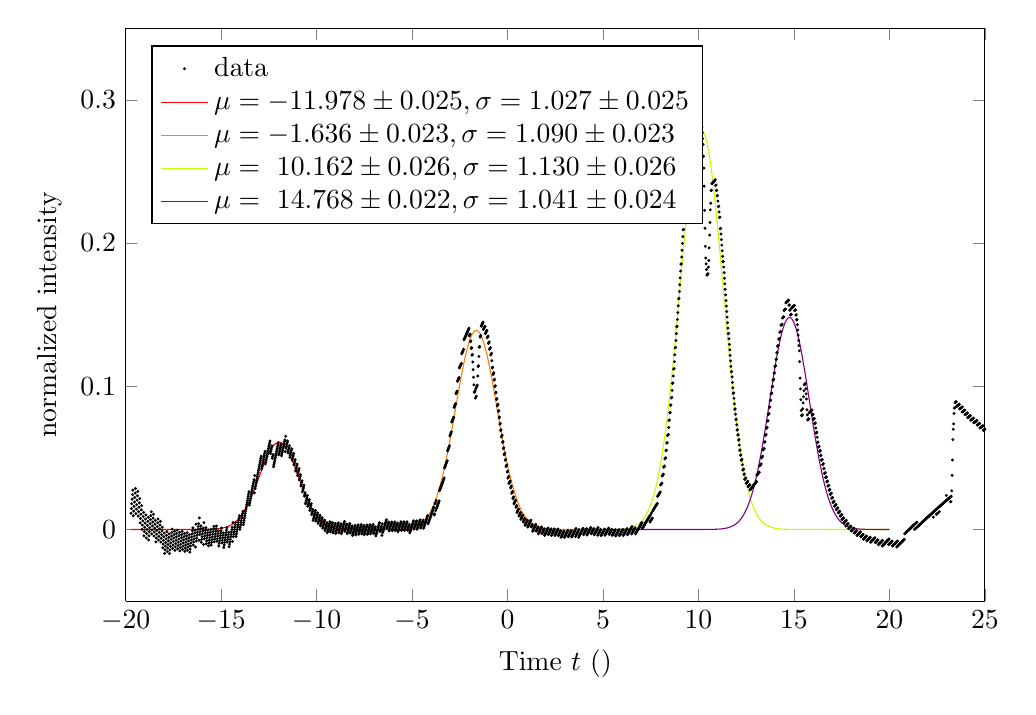
\begin{tikzpicture}

\begin{axis}[%
width=0.9\textwidth,
height=0.6\textwidth,
at={(0\textwidth,0\textwidth)},
scale only axis,
separate axis lines,
xmin=-20,
xmax=25,
xlabel={Time $t ~ (\milli\second)$},
ymin=-0.05,
ymax=0.35,
ylabel={normalized intensity},
tick label style={/pgf/number format/fixed},
legend style={at={(0.03,0.97)},anchor=north west,legend cell align=left,align=left,draw=black}
]
\addplot [color=black,only marks,mark=*,mark options={solid}, mark size=0.3]
  table[row sep=crcr]{%
-19.72	0.0113490213171509\\
-19.7	0.0146286297879102\\
-19.68	0.0178856918295456\\
-19.66	0.0211204388074118\\
-19.64	0.0243330989318701\\
-19.62	0.0275238973118875\\
-19.6	0.00962116592074702\\
-19.58	0.0128373330832249\\
-19.56	0.0160318347720345\\
-19.54	0.0192048888402883\\
-19.52	0.0223567102299124\\
-19.5	0.025487511020114\\
-19.48	0.0285975004748796\\
-19.46	0.011084478389311\\
-19.44	0.014218759458427\\
-19.42	0.0173324107670688\\
-19.4	0.0204256349973632\\
-19.38	0.0234986321848776\\
-19.36	0.0265515997616652\\
-19.34	0.00936774786095873\\
-19.32	0.0124440193596923\\
-19.3	0.0155004330801446\\
-19.28	0.0185371803592649\\
-19.26	0.0215544500835737\\
-19.24	0.00464533543700518\\
-19.22	0.00768500040363651\\
-19.2	0.0107053539309715\\
-19.18	0.0137065791500804\\
-19.16	0.0166888568836528\\
-19.14	4.5412995895e-05\\
-19.12	0.00304922749708203\\
-19.1	0.00603425511950606\\
-19.08	0.00900067124705572\\
-19.06	0.0119486490871827\\
-19.04	-0.00443775088946996\\
-19.02	-0.00146904810169679\\
-19	0.00148137169996054\\
-18.98	0.00441367657960934\\
-18.96	0.00732803254761139\\
-18.94	0.0102246035918596\\
-18.92	-0.00587522614327773\\
-18.9	-0.00295871235777878\\
-18.88	-5.98361473311826e-05\\
-18.86	0.00282156169145376\\
-18.84	0.00568563845151471\\
-18.82	0.00853254954391214\\
-18.8	-0.00729109018116914\\
-18.78	-0.00442497537857989\\
-18.76	-0.00157588631509675\\
-18.74	0.00125632796392927\\
-18.72	0.00407181663371414\\
-18.7	0.00687072711618109\\
-18.68	0.00965320510564749\\
-18.66	0.0124193945940503\\
-18.64	-0.00306816510618457\\
-18.62	-0.000283497000878707\\
-18.6	0.00248501078673724\\
-18.58	0.00523749822766773\\
-18.56	0.00797410368095941\\
-18.54	0.0106949639168404\\
-18.52	-0.00453796378527871\\
-18.5	-0.00179928493605241\\
-18.48	0.000923770713280536\\
-18.46	0.00363133617646472\\
-18.44	0.00632354296142057\\
-18.42	-0.00869589817472982\\
-18.4	-0.00598648660354351\\
-18.38	-0.00329231538568786\\
-18.36	-0.000613256583075206\\
-18.34	0.00205081631422721\\
-18.32	0.00470002840787065\\
-18.3	0.00733450341076569\\
-18.28	-0.00741485802376451\\
-18.26	-0.00476378333859984\\
-18.24	-0.00212733492439421\\
-18.22	0.0004946076420832\\
-18.2	0.00310216346555181\\
-18.18	0.00569545035021635\\
-18.16	-0.00882412923740028\\
-18.14	-0.00621480611594305\\
-18.12	-0.00361964620254862\\
-18.1	-0.0010385347764843\\
-18.08	0.00152864164720401\\
-18.06	-0.0127979708464887\\
-18.04	-0.0102152840532097\\
-18.02	-0.00764642959643713\\
-18	-0.00509129692856325\\
-17.98	-0.00254977667698397\\
-17.96	-0.0166887899723394\\
-17.94	-0.0141322607427152\\
-17.92	-0.0115892442270336\\
-17.9	-0.00905963385236053\\
-17.88	-0.00654332416366521\\
-17.86	-0.00404021080920458\\
-17.84	-0.00155019052613103\\
-17.82	-0.0154514096693781\\
-17.8	-0.0129468742936367\\
-17.78	-0.0104553382603616\\
-17.76	-0.00797670089909408\\
-17.74	-0.00551086257633182\\
-17.72	-0.00305772468221388\\
-17.7	-0.0167561765467166\\
-17.68	-0.0142889859540563\\
-17.66	-0.0118344061433076\\
-17.64	-0.00939234094351149\\
-17.62	-0.00696269515924652\\
-17.6	-0.00454537455828929\\
-17.58	-0.00214028585946391\\
-17.56	0.000252663279324494\\
-17.54	-0.0131976489926298\\
-17.52	-0.0107911033698289\\
-17.5	-0.00839661418002757\\
-17.48	-0.00601409131336217\\
-17.46	-0.00364344555584806\\
-17.44	-0.00128458857827618\\
-17.42	-0.0145458303147272\\
-17.4	-0.012173796567077\\
-17.38	-0.00981347195228643\\
-17.36	-0.00746477024590719\\
-17.34	-0.00512760606814555\\
-17.32	-0.00280189487354621\\
-17.3	-0.000487552940824809\\
-17.28	-0.0135411819376614\\
-17.26	-0.011214071360409\\
-17.24	-0.0088982548489589\\
-17.22	-0.00659365064115303\\
-17.2	-0.00430017776227709\\
-17.18	-0.00201775601560361\\
-17.16	-0.0148939772756931\\
-17.14	-0.0125991694049776\\
-17.12	-0.0103153405170759\\
-17.1	-0.00804241226598235\\
-17.08	-0.00578030704948973\\
-17.06	-0.00352894800038261\\
-17.04	-0.00128825897775808\\
-17.02	-0.0139694804473993\\
-17	-0.0117167779395506\\
-16.98	-0.00947467721697093\\
-16.96	-0.00724310386529226\\
-16.94	-0.00502198416506849\\
-16.92	-0.0028112450836939\\
-16.9	-0.0153256791831096\\
-16.88	-0.0131032762104188\\
-16.86	-0.0108911882940788\\
-16.84	-0.00868934403535349\\
-16.82	-0.00649767269306167\\
-16.8	-0.0043161041760249\\
-16.78	-0.0021445690356201\\
-16.76	-0.0144755056824661\\
-16.74	-0.01229264779899\\
-16.72	-0.0101197611752051\\
-16.7	-0.0079567778899392\\
-16.68	-0.00580363063762523\\
-16.66	-0.00366025272134496\\
-16.64	-0.0158341005894771\\
-16.62	-0.0136797202700938\\
-16.6	-0.0115350495343973\\
-16.58	-0.00940002313333821\\
-16.56	-0.00727457640132223\\
-16.54	-0.00515864524970611\\
-16.52	-0.00305216616037551\\
-16.5	-0.000955076179409931\\
-16.48	0.00113268708916558\\
-16.46	-0.0108280935880622\\
-16.44	-0.00872965375974788\\
-16.42	-0.00664048551428165\\
-16.4	-0.0045605277783618\\
-16.38	-0.00248972001403347\\
-16.36	-0.000428002212836454\\
-16.34	-0.0122416387079431\\
-16.32	0.00366840092112375\\
-16.3	-0.00810647405178644\\
-16.28	-0.00605238824606169\\
-16.26	-0.00400722229378903\\
-16.24	-0.00197091845379394\\
-16.22	5.65805176796497e-05\\
-16.2	0.00207533137231286\\
-16.18	0.00408539037498967\\
-16.16	-0.00752843582374885\\
-16.14	0.0080796554812036\\
-16.12	-0.00349679578352746\\
-16.1	-0.00149388472930334\\
-16.08	0.000500493365121479\\
-16.06	0.00248639268312323\\
-16.04	-0.00898932403697583\\
-16.02	-0.00699361205535554\\
-16	-0.00500633144645612\\
-15.98	-0.00302742912191833\\
-15.96	-0.00105685243826459\\
-15.94	0.000905450807749508\\
-15.92	-0.0104356738511522\\
-15.9	0.00480544362618196\\
-15.88	-0.00650018808242359\\
-15.86	-0.00454473556117563\\
-15.84	-0.00259740882429216\\
-15.82	-0.000658157553376615\\
-15.8	0.00127306815524875\\
-15.78	-0.00991952012894726\\
-15.76	-0.00797899585756756\\
-15.74	-0.00604645354519229\\
-15.72	-0.00412184426955031\\
-15.7	-0.00220511950747304\\
-15.68	-0.000296231130831437\\
-15.66	-0.0113613019402197\\
-15.64	-0.00944335443969124\\
-15.62	-0.00753320119695622\\
-15.6	-0.00563079501937636\\
-15.58	-0.00373608909465228\\
-15.56	-0.0018490369869959\\
-15.54	3.04073666429483e-05\\
-15.52	-0.0108938348312233\\
-15.5	-0.00900556714619882\\
-15.48	-0.00712486701720394\\
-15.46	-0.00525168926334341\\
-15.44	-0.00338598906278187\\
-15.42	-0.00152772194918582\\
-15.4	0.000323156191794793\\
-15.38	0.00216668912600293\\
-15.36	-0.00860463769700526\\
-15.34	-0.00675251370582397\\
-15.32	-0.00490769702213356\\
-15.3	-0.00307014470339606\\
-15.28	-0.00123981414300833\\
-15.26	0.000583336932979628\\
-15.24	0.00239935046910222\\
-15.22	-0.00823912856527209\\
-15.2	-0.00641474228960659\\
-15.18	-0.00459745733548989\\
-15.16	-0.00278723253616087\\
-15.14	-0.000984027042552293\\
-15.12	-0.0115234521760359\\
-15.1	-0.00971207402472429\\
-15.08	-0.00790767967600092\\
-15.06	-0.00611022903234071\\
-15.04	-0.00431968230270208\\
-15.02	-0.00253599999960685\\
-15	-0.000759142936249901\\
-14.98	0.00101092777635614\\
-14.96	-0.00938703889301085\\
-14.94	-0.00760900327626013\\
-14.92	-0.0058377204611777\\
-14.9	-0.00407315226205585\\
-14.88	-0.00231526078066602\\
-14.86	-0.0126189964566115\\
-14.84	-0.0108533259656425\\
-14.82	-0.00909429928876104\\
-14.8	-0.00734187920787877\\
-14.78	-0.0055960287824881\\
-14.76	-0.0038567113470811\\
-14.74	-0.00212389050859385\\
-14.72	-0.00039753014388122\\
-14.7	0.00132240560278041\\
-14.68	-0.00883266729304855\\
-14.66	-0.00710515054624672\\
-14.64	-0.00538402765208335\\
-14.62	-0.00366926338568008\\
-14.6	-0.00196082278053944\\
-14.58	-0.0120264201982527\\
-14.56	-0.010310571306571\\
-14.54	-0.00860101588329054\\
-14.52	-0.00689771957255969\\
-14.5	-0.00520064826824473\\
-14.48	-0.00350976811166359\\
-14.46	-0.00182504548934603\\
-14.44	-0.000146447030818786\\
-14.42	0.00152606039358716\\
-14.4	-0.00839827509631741\\
-14.38	0.00485293346767435\\
-14.36	-0.00504487575918766\\
-14.34	-0.00337723766127351\\
-14.32	-0.00171559742709482\\
-14.3	-5.99229581395022e-05\\
-14.28	0.00158981761536692\\
-14.26	0.00323365593649394\\
-14.24	0.00487162342362013\\
-14.22	-0.00491574583938936\\
-14.2	-0.00327073332999528\\
-14.18	-0.00163156514054363\\
-14.16	1.78961930052957e-06\\
-14.14	0.00162936162245442\\
-14.12	0.00325118132632751\\
-14.1	0.0048672789747104\\
-14.08	0.00647768459964426\\
-14.06	0.00808242802327153\\
-14.04	0.00968153885966472\\
-14.02	3.95356816020875e-05\\
-14	0.00164551406342961\\
-13.98	0.00324588445876561\\
-13.96	0.00484067599460325\\
-13.94	0.00642991759647449\\
-13.92	0.00801363799018684\\
-13.9	0.00959186570354598\\
-13.88	0.0111646290680574\\
-13.86	0.0127319562206127\\
-13.84	0.00321852538723799\\
-13.82	0.00479255295158199\\
-13.8	0.00636116741802306\\
-13.78	0.00792439646909027\\
-13.76	0.00948226759877591\\
-13.74	0.0110348081141356\\
-13.72	0.0125820451368767\\
-13.7	0.014124005604926\\
-13.68	0.0156607162739857\\
-13.66	0.0171922037190699\\
-13.64	0.0187184943360279\\
-13.62	0.0202396143430515\\
-13.6	0.021755589782168\\
-13.58	0.0232664465207149\\
-13.56	0.0247722102528045\\
-13.54	0.0262729065007702\\
-13.52	0.0169659890678956\\
-13.5	0.0184731888698375\\
-13.48	0.0199753412723157\\
-13.46	0.021472471400843\\
-13.44	0.0229646042143453\\
-13.42	0.0244517645065431\\
-13.4	0.0259339769073131\\
-13.38	0.0274112658840415\\
-13.36	0.0288836557429599\\
-13.34	0.0303511706304719\\
-13.32	0.0318138345344624\\
-13.3	0.0332716712855978\\
-13.28	0.034724704558611\\
-13.26	0.0255814519161426\\
-13.24	0.0376164545971659\\
-13.22	0.0284953851740578\\
-13.2	0.0299451970320994\\
-13.18	0.031390269980936\\
-13.16	0.0328306270361793\\
-13.14	0.0342662910645453\\
-13.12	0.0356972847850567\\
-13.1	0.0371236307702332\\
-13.08	0.0385453514472711\\
-13.06	0.0399624690992096\\
-13.04	0.0413750058660884\\
-13.02	0.0427829837460917\\
-13	0.0441864245966834\\
-12.98	0.0455853501357304\\
-12.96	0.046979781942615\\
-12.94	0.0483697414593363\\
-12.92	0.0497552499916025\\
-12.9	0.0511363287099121\\
-12.88	0.0422142268968264\\
-12.86	0.0436014250726385\\
-12.84	0.0449842086768742\\
-12.82	0.0463625985741493\\
-12.8	0.047736615497711\\
-12.78	0.0491062800504696\\
-12.76	0.0504716127060207\\
-12.74	0.0518326338096592\\
-12.72	0.0531893635793816\\
-12.7	0.0545418221068807\\
-12.68	0.0457383092441056\\
-12.66	0.0470967364148145\\
-12.64	0.0484509065830958\\
-12.62	0.049800839555894\\
-12.6	0.0511465550173755\\
-12.58	0.0524880725298801\\
-12.56	0.0538254115348594\\
-12.54	0.0551585913538117\\
-12.52	0.0564876311892037\\
-12.5	0.0578125501253866\\
-12.48	0.0591333671295022\\
-12.46	0.0604501010523821\\
-12.44	0.0617627706294381\\
-12.42	0.0531040688909196\\
-12.4	0.0544225442128785\\
-12.38	0.0557369680644454\\
-12.36	0.0570473589225835\\
-12.34	0.0583537351519825\\
-12.32	0.0497577583217639\\
-12.3	0.0510698273284017\\
-12.28	0.0523778944488993\\
-12.26	0.0438244983980095\\
-12.24	0.0451381588665604\\
-12.22	0.0464478303365429\\
-12.2	0.0477535307807253\\
-12.18	0.0490552780639778\\
-12.16	0.0503530899440805\\
-12.14	0.0516469840725258\\
-12.12	0.0529369779953116\\
-12.1	0.0542230891537281\\
-12.08	0.0555053348851378\\
-12.06	0.0567837324237495\\
-12.04	0.0580582989013807\\
-12.02	0.0593290513482227\\
-12	0.0605960066935868\\
-11.98	0.0521876269395064\\
-11.96	0.0534600220940922\\
-11.94	0.0547286317093472\\
-11.92	0.0559934724889115\\
-11.9	0.057254561038211\\
-11.88	0.058511913865175\\
-11.86	0.0597655473809529\\
-11.84	0.0514340031853212\\
-11.82	0.0526929637014756\\
-11.8	0.0539482161106306\\
-11.78	0.0551997766074138\\
-11.76	0.0564476612922\\
-11.74	0.0576918861717939\\
-11.72	0.0589324671601111\\
-11.7	0.0601694200788493\\
-11.68	0.061402760658156\\
-11.66	0.0626325045372885\\
-11.64	0.0544026942073453\\
-11.62	0.0650812643015455\\
-11.6	0.0568690010268786\\
-11.58	0.0580967905986499\\
-11.56	0.0593210247719567\\
-11.54	0.0605417188068905\\
-11.52	0.0617588878762511\\
-11.5	0.0536022725368329\\
-11.48	0.0548245384905001\\
-11.46	0.0560432896798068\\
-11.44	0.057258541082866\\
-11.42	0.058470307592721\\
-11.4	0.050368491186442\\
-11.38	0.0515852613712054\\
-11.36	0.0527985567709579\\
-11.34	0.0540083920885878\\
-11.32	0.0552147819440647\\
-11.3	0.0564177408750234\\
-11.28	0.0483782370955514\\
-11.26	0.0495861043302835\\
-11.24	0.050790550551431\\
-11.22	0.0519915901123817\\
-11.2	0.0531892372862535\\
-11.18	0.0452027636088498\\
-11.16	0.0464052306931446\\
-11.14	0.0476043152089866\\
-11.12	0.0488000312494857\\
-11.1	0.0408577042990004\\
-11.08	0.0420581582503964\\
-11.06	0.0432552535511991\\
-11.04	0.0444490041172215\\
-11.02	0.0456394237874214\\
-11	0.0377486837179972\\
-10.98	0.0389437570857037\\
-10.96	0.0401355092868466\\
-10.94	0.041323953987139\\
-10.92	0.0425091047773379\\
-10.9	0.0346691919206783\\
-10.88	0.0358589142661189\\
-10.86	0.037045352334932\\
-10.84	0.0382285195485711\\
-10.82	0.0304309379400031\\
-10.8	0.0316186002892923\\
-10.78	0.0328030014145382\\
-10.76	0.0339841545704254\\
-10.74	0.0262283884300064\\
-10.72	0.0274139619456966\\
-10.7	0.0285962971175474\\
-10.68	0.0297754070359719\\
-10.66	0.0309513047208387\\
-10.64	0.0232444068203135\\
-10.62	0.0244246482857305\\
-10.6	0.0256016870431285\\
-10.58	0.0179280408240977\\
-10.56	0.0191093551458931\\
-10.54	0.0202874763648334\\
-10.52	0.0214624172501272\\
-10.5	0.0226341905029031\\
-10.48	0.023802808756662\\
-10.46	0.0161842150694189\\
-10.44	0.0173570325419601\\
-10.42	0.0185267044291183\\
-10.4	0.0196932432097647\\
-10.38	0.0208566612967648\\
-10.36	0.0132849797073925\\
-10.34	0.0144525256488223\\
-10.32	0.0156169602091704\\
-10.3	0.0167782956501167\\
-10.28	0.017936544168913\\
-10.26	0.0104111136324202\\
-10.24	0.0115734203157184\\
-10.22	0.0127326492887891\\
-10.2	0.0138888126010525\\
-10.18	0.0064019391007718\\
-10.16	0.007562095303286\\
-10.14	0.00871919503950858\\
-10.12	0.00987325021320951\\
-10.1	0.0110242726663392\\
-10.08	0.0121722741794292\\
-10.06	0.0133172664719915\\
-10.04	0.00588934173510958\\
-10.02	0.00703825492710497\\
-10	0.00818416783035336\\
-9.98	0.00932709202401827\\
-9.96	0.0104670390276705\\
-9.94	0.011604020301673\\
-9.92	0.00422716834451875\\
-9.9	0.00536800302916562\\
-9.88	0.00650588074049963\\
-9.86	0.00764081280260209\\
-9.84	0.00877281048172118\\
-9.82	0.00990188498663946\\
-9.8	0.00257529573800852\\
-9.78	0.00370815781895384\\
-9.76	0.00483810531100037\\
-9.74	0.00596514929057124\\
-9.72	0.00708930077795167\\
-9.7	0.00821057073764253\\
-9.68	0.000933452875992113\\
-9.66	0.0020584461776586\\
-9.64	0.00318056637017605\\
-9.62	0.00429982428946674\\
-9.6	0.00541623071694908\\
-9.58	0.00652979637987705\\
-9.56	-0.000698623242003205\\
-9.54	0.000418603077952162\\
-9.52	0.00153299688927844\\
-9.5	0.00264456879429997\\
-9.48	0.00375332934240857\\
-9.46	0.00485928903039412\\
-9.44	-0.00232118787803826\\
-9.42	-0.00121162871828995\\
-9.4	-0.000104862321328003\\
-9.38	0.000999121688226801\\
-9.36	0.00210033363433981\\
-9.34	0.00319878378988048\\
-9.32	0.00429448237693764\\
-9.3	0.00538743956713328\\
-9.28	-0.00173326290251374\\
-9.26	-0.000636770549250709\\
-9.24	0.000456988215852716\\
-9.22	0.00154802344805804\\
-9.2	0.0026363451532877\\
-9.18	0.00372196328842656\\
-9.16	0.00480488776162313\\
-9.14	-0.00226335412124512\\
-9.12	-0.00117695492717718\\
-9.1	-9.32417979875311e-05\\
-9.08	0.0009877950621201\\
-9.06	0.0020661654012859\\
-9.04	0.00314187892028206\\
-9.02	0.00421494527279986\\
-9	-0.00280173671421746\\
-8.98	-0.00172525461321338\\
-8.96	-0.00065141228574972\\
-8.94	0.000419799813351385\\
-8.92	0.00148839118322208\\
-8.9	0.00255437127722591\\
-8.88	0.00361774950323224\\
-8.86	0.00467853522389017\\
-8.84	-0.0022815143579642\\
-8.82	-0.0012173726055642\\
-8.8	-0.000155816222136451\\
-8.78	0.000903164050848115\\
-8.76	0.0019595774276816\\
-8.74	0.00301343307868296\\
-8.72	0.00406474013045988\\
-8.7	-0.00284558427250214\\
-8.68	-0.00179097731642175\\
-8.66	-0.000738912011252424\\
-8.64	0.000310620668985573\\
-8.62	0.00135762970750253\\
-8.6	0.00240212404499296\\
-8.58	0.00344411257988719\\
-8.56	0.00448360416860027\\
-8.54	0.00552060762577955\\
-8.52	-0.00132935135700052\\
-8.5	-0.000289106984217025\\
-8.48	0.000748655913646146\\
-8.46	0.00178394605525889\\
-8.44	0.0028167721184128\\
-8.42	0.00384714274026177\\
-8.4	-0.00296056287994007\\
-8.38	-0.0019270027017122\\
-8.36	-0.000895891426845985\\
-8.34	0.000132779488366985\\
-8.32	0.00115901854785794\\
-8.3	0.00218283421601073\\
-8.28	0.00320423491789346\\
-8.26	0.00422322903948458\\
-8.24	-0.00253173893985048\\
-8.22	-0.00150960949204015\\
-8.2	-0.000489880305539536\\
-8.18	0.000527456915834557\\
-8.16	0.00154241042999481\\
-8.14	0.00255498845680679\\
-8.12	-0.00415910160325916\\
-8.1	-0.00314343723985799\\
-8.08	-0.00213014215554819\\
-8.06	-0.0011192082179301\\
-8.04	-0.000110627331860957\\
-8.02	0.000895608560759986\\
-8	0.00189950748119982\\
-7.98	0.00290107741410595\\
-7.96	-0.00376197887453666\\
-7.94	-0.00275737437153811\\
-7.92	-0.00175509285248454\\
-7.9	-0.000755126416832619\\
-7.88	0.000242532800094564\\
-7.86	0.00123789262731178\\
-7.84	0.00223096085837249\\
-7.82	0.00322174525156993\\
-7.8	-0.00339119491619821\\
-7.78	-0.00239742651540298\\
-7.76	-0.00140593614497431\\
-7.74	-0.000416716127519923\\
-7.72	0.000570241179812636\\
-7.7	0.00155494338552953\\
-7.68	0.00253739806398434\\
-7.66	0.00351761275556872\\
-7.64	-0.00304610507122649\\
-7.62	-0.00206295576707438\\
-7.6	-0.00108204083024743\\
-7.58	-0.000103352798203948\\
-7.56	0.000873115758324494\\
-7.54	0.0018473722355169\\
-7.52	0.00281942399664725\\
-7.5	-0.00370102780538462\\
-7.48	-0.0027260878459241\\
-7.46	-0.00175334712050668\\
-7.44	-0.000782798341275592\\
-7.42	0.000185565747380712\\
-7.4	0.00115175236900888\\
-7.38	0.00211576871526609\\
-7.36	0.00307762194609562\\
-7.34	-0.00339523812957565\\
-7.32	-0.00243054389251407\\
-7.3	-0.00146800746335085\\
-7.28	-0.000507621754763488\\
-7.26	0.000450620289489279\\
-7.24	0.0014067256947361\\
-7.22	0.00236070145556322\\
-7.2	0.003312554535981\\
-7.18	-0.00311354300544786\\
-7.16	-0.00215889504498623\\
-7.14	-0.00120636462483881\\
-7.12	-0.000255944850945822\\
-7.1	0.000692371140779025\\
-7.08	0.0016385901846141\\
-7.06	0.00258271908518903\\
-7.04	0.00352476461764573\\
-7.02	-0.0028553787256731\\
-7	-0.00191058340496864\\
-6.98	-0.000967866473010615\\
-6.96	-2.72212220595591e-05\\
-6.94	0.000911359026711911\\
-6.92	0.00184788092337662\\
-6.9	-0.00449660985154776\\
-6.88	-0.00355737880102613\\
-6.86	-0.00262020120348216\\
-6.84	-0.00168507047461852\\
-6.82	-0.0007519800583351\\
-6.8	0.000179076573422199\\
-6.78	0.00110810592081079\\
-6.76	0.00203511445623961\\
-6.74	0.0029601086245179\\
-6.72	0.00388309484300231\\
-6.7	0.00480407950174166\\
-6.68	-0.00148183633374188\\
-6.66	-0.000558190800959313\\
-6.64	0.000363457813509771\\
-6.62	0.00128311583745044\\
-6.6	0.00220078957186443\\
-6.58	-0.00405533855571583\\
-6.56	0.0040302092430472\\
-6.54	-0.0022167232310526\\
-6.52	-0.00130037885852596\\
-6.5	-0.000386001719018036\\
-6.48	0.000526414374905859\\
-6.46	0.00143687558468353\\
-6.44	0.00234538804589168\\
-6.42	0.00325195786838106\\
-6.4	0.00415659113641142\\
-6.38	0.00505929390878512\\
-6.36	0.00596007221898009\\
-6.34	0.00685893207528265\\
-6.32	0.000668421457066914\\
-6.3	0.00156985547942323\\
-6.28	0.00246937534733715\\
-6.26	0.00336698701183591\\
-6.24	0.00426269639922838\\
-6.22	0.00515650941123191\\
-6.2	-0.00100086997614013\\
-6.18	-0.000104519782180068\\
-6.16	0.00078993827032714\\
-6.14	0.00168251002716846\\
-6.12	0.00257320130999872\\
-6.1	0.00346201791646461\\
-6.08	0.00434896562032938\\
-6.06	0.00523405017159462\\
-6.04	-0.000881896806922189\\
-6.02	5.68546373902468e-06\\
-6	0.000891408690145368\\
-5.98	0.00177527856829884\\
-5.96	0.00265730077087956\\
-5.94	0.0035374809473655\\
-5.92	0.00441582472415081\\
-5.9	0.0052923377046632\\
-5.88	-0.000782855471291422\\
-5.86	9.61166084543219e-05\\
-5.84	0.000973261879407827\\
-5.82	0.00184858589284598\\
-5.8	0.00272209417750058\\
-5.78	0.0035937922396726\\
-5.76	0.00446368556334698\\
-5.74	-0.00157563858684706\\
-5.72	-0.000703322403239337\\
-5.7	0.00016719294146883\\
-5.68	0.00103591288058758\\
-5.66	0.00190284282551634\\
-5.64	0.00276798816585455\\
-5.62	0.00363135426951144\\
-5.6	0.00449294648281418\\
-5.58	0.00535277013061752\\
-5.56	-0.000642887893821831\\
-5.54	0.000219320046024096\\
-5.52	0.00107976317945246\\
-5.5	0.00193844678263255\\
-5.48	0.00279537611064806\\
-5.46	0.00365055639760248\\
-5.44	0.00450399285672265\\
-5.42	0.00535569068046349\\
-5.4	-0.000601155541302356\\
-5.38	0.000252890342415601\\
-5.36	0.00110520124190228\\
-5.34	0.00195578230255344\\
-5.32	0.0028046386493642\\
-5.3	0.00365177538703032\\
-5.28	0.0044971976000483\\
-5.26	0.00534091035281514\\
-5.24	-0.00057774172734959\\
-5.22	0.000268283605587394\\
-5.2	0.00111260302541594\\
-5.18	0.00195522155103223\\
-5.16	0.00279614418158969\\
-5.14	0.00363537589659613\\
-5.12	-0.00225361265712598\\
-5.1	-0.00141210017804339\\
-5.08	-0.000572275117863397\\
-5.06	0.000265867458416613\\
-5.04	0.00110233246649971\\
-5.02	0.00193712480288422\\
-5	0.00277024934495673\\
-4.98	0.00360171095108563\\
-4.96	0.00443151446071355\\
-4.94	0.00525966469444938\\
-4.92	0.0060861664541596\\
-4.9	0.000245997842006074\\
-4.88	0.00107474194543911\\
-4.86	0.00190184090124834\\
-4.84	0.00272729946896566\\
-4.82	0.00355112238970701\\
-4.8	0.00437331438626176\\
-4.78	0.00519388016318134\\
-4.76	0.00601282440686657\\
-4.74	0.00020901946422669\\
-4.72	0.00103017272957617\\
-4.7	0.00184970769564985\\
-4.68	0.00266762900788031\\
-4.66	0.00348394129386398\\
-4.64	0.00429864916344647\\
-4.62	0.00511175720880686\\
-4.6	0.00592327000454285\\
-4.58	0.0067331921077548\\
-4.56	0.000968955396261961\\
-4.54	0.00178105245999349\\
-4.52	0.00259156195381016\\
-4.5	0.00340048839537388\\
-4.48	0.00420783628514887\\
-4.46	0.00501361010648294\\
-4.44	0.00581781432568951\\
-4.42	0.00662045339212769\\
-4.4	0.000891410236560808\\
-4.38	0.0016961922915556\\
-4.36	0.00249941223103012\\
-4.34	0.00330107446615724\\
-4.32	0.00410118339144339\\
-4.3	0.00489974338480814\\
-4.28	0.00569675880766141\\
-4.26	0.00649223400498167\\
-4.24	0.00728617330539327\\
-4.22	0.00807858102124304\\
-4.2	0.00886946144867662\\
-4.18	0.00965881886771469\\
-4.16	0.00397898863737634\\
-4.14	0.00477045218927574\\
-4.12	0.00556039560583554\\
-4.1	0.00634882313088425\\
-4.08	0.00713573899239606\\
-4.06	0.007921147402564\\
-4.04	0.00870505255787468\\
-4.02	0.00948745863917977\\
-4	0.0102683698117703\\
-3.98	0.0110477902254476\\
-3.96	0.0118257240145959\\
-3.94	0.0126021752982542\\
-3.92	0.013377148180186\\
-3.9	0.0141506467489512\\
-3.88	0.0149226750779763\\
-3.86	0.0156932372256233\\
-3.84	0.0100757290354897\\
-3.82	0.0108483556232233\\
-3.8	0.0179961669394223\\
-3.78	0.0187609046463314\\
-3.76	0.0131574702416971\\
-3.74	0.0202860456902674\\
-3.72	0.0146896157629351\\
-3.7	0.0154535211978772\\
-3.68	0.0162159870223683\\
-3.66	0.0169770171732926\\
-3.64	0.0177366155731221\\
-3.62	0.0184947861299819\\
-3.6	0.0192515327377151\\
-3.58	0.0200068592759487\\
-3.56	0.027078442064286\\
-3.54	0.0278260852201719\\
-3.52	0.028572328947982\\
-3.5	0.0293171770464552\\
-3.48	0.0300606333005232\\
-3.46	0.0308027014813749\\
-3.44	0.0315433853465168\\
-3.42	0.0322826886398365\\
-3.4	0.0330206150916633\\
-3.38	0.0337571684188298\\
-3.36	0.0344923523247332\\
-3.34	0.0352261704993952\\
-3.32	0.0359586266195229\\
-3.3	0.0429449858787723\\
-3.28	0.0436699902761594\\
-3.26	0.0443936523432423\\
-3.24	0.0451159756805323\\
-3.22	0.0458369638756064\\
-3.2	0.0465566205031663\\
-3.18	0.047274949125095\\
-3.16	0.0479919532905153\\
-3.14	0.0549252336826705\\
-3.12	0.0556349304738465\\
-3.1	0.0563433219673704\\
-3.08	0.0570504116390217\\
-3.06	0.0577562029521833\\
-3.04	0.0584606993578963\\
-3.02	0.0653536154508687\\
-3	0.0660509144714051\\
-2.98	0.0667469373156105\\
-2.96	0.0674416873633209\\
-2.94	0.0681351679823815\\
-2.92	0.0749940886046689\\
-2.9	0.0756804645824157\\
-2.88	0.0763655895040067\\
-2.86	0.0770494666678618\\
-2.84	0.0777320993607503\\
-2.82	0.0784134908578419\\
-2.8	0.0852330201266066\\
-2.78	0.085907412885573\\
-2.76	0.0865805824147614\\
-2.74	0.0872525319219241\\
-2.72	0.0879232646035418\\
-2.7	0.0947096106002778\\
-2.68	0.0953734338829615\\
-2.66	0.0960360579651167\\
-2.64	0.0966974859774786\\
-2.62	0.103456655357128\\
-2.6	0.104111247570094\\
-2.58	0.104764661058483\\
-2.56	0.105416898888644\\
-2.54	0.106067964116241\\
-2.52	0.112794609039444\\
-2.5	0.113438925062917\\
-2.48	0.114082085502092\\
-2.46	0.114724093349835\\
-2.44	0.115364951588621\\
-2.42	0.116004663190582\\
-2.4	0.122693619945513\\
-2.38	0.123326681209317\\
-2.36	0.123958612484103\\
-2.34	0.124589416680996\\
-2.32	0.125219096701068\\
-2.3	0.125847655435382\\
-2.28	0.132499405449413\\
-2.26	0.133121410764221\\
-2.24	0.133742311080432\\
-2.22	0.134362109229831\\
-2.2	0.134980808034479\\
-2.18	0.135598410306745\\
-2.16	0.136214918849356\\
-2.14	0.136830336455431\\
-2.12	0.13744466590853\\
-2.1	0.138057909982687\\
-2.08	0.138670071442455\\
-2.06	0.139281153042946\\
-2.04	0.13989115752987\\
-2.02	0.140500087639578\\
-2	0.135143417947007\\
-1.98	0.135754421290244\\
-1.96	0.136364351005208\\
-1.94	0.131021300912085\\
-1.92	0.131633283174749\\
-1.9	0.126300659659864\\
-1.88	0.126914675912743\\
-1.86	0.121592431137109\\
-1.84	0.12220846297158\\
-1.82	0.116896549392322\\
-1.8	0.111591857597896\\
-1.78	0.106294368574653\\
-1.76	0.101004063372569\\
-1.74	0.0957209231049737\\
-1.72	0.09635113070836\\
-1.7	0.096980241985073\\
-1.68	0.0917102744488459\\
-1.66	0.0982351865276024\\
-1.64	0.0929712280344224\\
-1.62	0.0994857785788749\\
-1.6	0.100109449207242\\
-1.58	0.100732039838965\\
-1.56	0.107227059352376\\
-1.54	0.113712893930083\\
-1.52	0.114324164377799\\
-1.5	0.120795741237278\\
-1.48	0.127258197026177\\
-1.46	0.127858254915207\\
-1.44	0.134306559202404\\
-1.42	0.134900539058609\\
-1.4	0.135493497319811\\
-1.38	0.141922697075123\\
-1.36	0.142509626992411\\
-1.34	0.143095549716256\\
-1.32	0.143680467729743\\
-1.3	0.144264383507743\\
-1.28	0.144847299516945\\
-1.26	0.139615811537088\\
-1.24	0.140200687239056\\
-1.22	0.140784563772404\\
-1.2	0.141367443587991\\
-1.18	0.141949329128607\\
-1.16	0.136736508118393\\
-1.14	0.13732033067754\\
-1.12	0.137903159573123\\
-1.1	0.138484997232277\\
-1.08	0.139065846074179\\
-1.06	0.133871518634309\\
-1.04	0.134454282157722\\
-1.02	0.135036057486021\\
-1	0.129854292669717\\
-0.98	0.13043796418529\\
-0.96	0.131020648153258\\
-0.94	0.125851369135094\\
-0.92	0.126435930990052\\
-0.9	0.127019505969745\\
-0.88	0.121862636570981\\
-0.86	0.12244807132885\\
-0.84	0.123032519908089\\
-0.82	0.1178879845895\\
-0.8	0.112750082007829\\
-0.78	0.113339187668923\\
-0.76	0.108210705821737\\
-0.74	0.108801622856091\\
-0.72	0.109391548822887\\
-0.7	0.104275232808721\\
-0.68	0.104866952691595\\
-0.66	0.0997599605502947\\
-0.64	0.100353458611976\\
-0.62	0.0952557494671222\\
-0.6	0.095851010090295\\
-0.58	0.0907625433054197\\
-0.56	0.0913595509916646\\
-0.54	0.0862802861684242\\
-0.52	0.0868790255371689\\
-0.5	0.0874767686708561\\
-0.48	0.0824093783010128\\
-0.46	0.0830088364307586\\
-0.44	0.0779505542077004\\
-0.42	0.0785517122137559\\
-0.4	0.0735024985292382\\
-0.38	0.0741053414062998\\
-0.36	0.0690651568823675\\
-0.34	0.0696696697385724\\
-0.32	0.0646384752258211\\
-0.3	0.0652446432817542\\
-0.28	0.0658498106369031\\
-0.26	0.0608302084453178\\
-0.24	0.0614370150467697\\
-0.22	0.0564263119743469\\
-0.2	0.0570347432912592\\
-0.18	0.0520329009468807\\
-0.16	0.0526429425576388\\
-0.14	0.0532519820491008\\
-0.12	0.0482615603625499\\
-0.1	0.0488721946270149\\
-0.08	0.0438905445494135\\
-0.06	0.0445027594065495\\
-0.04	0.0451139721039636\\
-0.02	0.0401436246614485\\
-0	0.0407564027197789\\
0.02	0.0357947389861965\\
0.04	0.0364090684614637\\
0.06	0.0370223958263018\\
0.08	0.0320719183457348\\
0.1	0.0326867821786151\\
0.12	0.033300645122981\\
0.14	0.0339135095023859\\
0.16	0.0289766729068843\\
0.18	0.0295910578692581\\
0.2	0.0302044454948599\\
0.22	0.0252786485949693\\
0.24	0.0258935421770775\\
0.26	0.0265074396649675\\
0.28	0.0215926180363137\\
0.3	0.0222080070009489\\
0.32	0.0228224011279338\\
0.34	0.0179184908592757\\
0.36	0.0185343621281502\\
0.38	0.0191492398296107\\
0.4	0.0197631262463864\\
0.42	0.0203760236541528\\
0.44	0.0154878665368469\\
0.46	0.0161022248951364\\
0.48	0.0167155955112734\\
0.5	0.0118381928279915\\
0.52	0.0124530103870376\\
0.54	0.0130668414838029\\
0.56	0.0136796883703588\\
0.58	0.0142915532918593\\
0.6	0.00942967425593699\\
0.62	0.0100429703313586\\
0.64	0.010655285717776\\
0.66	0.0112666226452582\\
0.68	0.011876983337051\\
0.7	0.0070304936008152\\
0.72	0.00764226987188321\\
0.74	0.0082530711793728\\
0.76	0.00886289973162713\\
0.78	0.00947175773025799\\
0.8	0.0100796473701705\\
0.82	0.00525078276727975\\
0.84	0.00586007169546943\\
0.86	0.00646839352498196\\
0.88	0.0070757504360649\\
0.9	0.00768214460235028\\
0.92	0.00286838462908023\\
0.94	0.0034761629433383\\
0.96	0.00408297976876404\\
0.98	0.00468883726450808\\
1	0.00529373758319374\\
1.02	0.00589768287094083\\
1.04	0.00650067526739073\\
1.06	0.001706536019349\\
1.08	0.00231089583615751\\
1.1	0.00291430399788362\\
1.12	0.00351676262998624\\
1.14	0.00411827385153196\\
1.16	0.00471883977521903\\
1.18	0.00531846250740109\\
1.2	0.00591714414811106\\
1.22	0.0065148867910847\\
1.24	0.00174472869958864\\
1.26	0.00234382052702986\\
1.28	0.00294197455848066\\
1.3	0.00353919287390503\\
1.32	-0.00121863278871492\\
1.34	-0.000620078867172857\\
1.36	-2.24594563387193e-05\\
1.38	0.000574227510084735\\
1.4	0.0011699840922389\\
1.42	0.00176481234413406\\
1.44	0.00235871431367074\\
1.46	0.0029516920426631\\
1.48	0.00354374756686093\\
1.5	-0.00119059899356766\\
1.52	-0.000597225554154202\\
1.54	-4.77314755653602e-06\\
1.56	0.000586760248699858\\
1.58	0.00117737665110562\\
1.6	0.00176707807018817\\
1.62	-0.00295075122079247\\
1.64	-0.00235974675274653\\
1.66	-0.00176965610703639\\
1.68	-0.00118047728619719\\
1.7	-0.000592208298649366\\
1.72	-4.84715867643537e-06\\
1.74	0.000581608113596088\\
1.76	0.00116715949222279\\
1.78	0.00175180894545901\\
1.8	-0.00294308940318189\\
1.82	-0.00235715404876413\\
1.84	-0.00177211949058598\\
1.86	-0.00118798377308393\\
1.88	-0.000604744946419045\\
1.9	-2.24010664551244e-05\\
1.92	0.000559049805262224\\
1.94	-0.0041175503479407\\
1.96	-0.00353482880183353\\
1.98	-0.00295299915211311\\
2	-0.00237205947276431\\
2.02	-0.00179200784338129\\
2.04	-0.00121284234914687\\
2.06	-0.000634561080812723\\
2.08	-5.71621346778795e-05\\
2.1	0.000519356387429615\\
2.12	0.0010949963781739\\
2.14	-0.00355710017199806\\
2.16	-0.00298020693564816\\
2.18	-0.00240419115560386\\
2.2	-0.00182905095124086\\
2.22	-0.00125478444737182\\
2.24	-0.00068138977422838\\
2.26	-0.000108865067440123\\
2.28	0.000462791531983586\\
2.3	-0.00416936821671321\\
2.32	-0.00359647391219409\\
2.34	-0.00302444666266211\\
2.36	-0.00245328462088001\\
2.38	-0.00188298594492076\\
2.4	-0.00131354879815015\\
2.42	-0.000744971349205814\\
2.44	-0.000177251771980247\\
2.46	0.000389611754398889\\
2.48	-0.00422077470029025\\
2.5	-0.00365268955991493\\
2.52	-0.00308545944634897\\
2.54	-0.00251908255014754\\
2.56	-0.0019535570670357\\
2.58	-0.00138888119788949\\
2.6	-0.000825053148717059\\
2.62	-0.000262071130640917\\
2.64	0.000300066640119834\\
2.66	-0.00428883722297724\\
2.68	-0.00372549367452346\\
2.7	-0.00316299337680026\\
2.72	-0.00260133455714073\\
2.74	-0.00204051544790973\\
2.76	-0.00148053428648698\\
2.78	-0.000921389315248433\\
2.8	-0.00549314585222449\\
2.82	-0.00493280914764549\\
2.84	-0.00437330765145183\\
2.86	-0.00381463961691964\\
2.88	-0.00325680330225908\\
2.9	-0.00269979697059819\\
2.92	-0.00214361888996417\\
2.94	-0.00158826733326722\\
2.96	-0.00103374057828276\\
2.98	-0.00558452689185729\\
3	-0.00502882376494562\\
3.02	-0.00447394448405536\\
3.04	-0.00391988733756521\\
3.06	-0.00336665061865959\\
3.08	-0.00281423262531133\\
3.1	-0.00226263166026475\\
3.12	-0.00171184603101948\\
3.14	-0.00116187404981316\\
3.16	-0.000612714033606077\\
3.18	-0.00514083315839842\\
3.2	-0.00459051264534382\\
3.22	-0.004041003172498\\
3.24	-0.00349230306709658\\
3.26	-0.00294441066103857\\
3.28	-0.00239732429087125\\
3.3	-0.00185104229777333\\
3.32	-0.00130556302753915\\
3.34	-0.000760884830562469\\
3.36	-0.00526860710253718\\
3.38	-0.00472278328833853\\
3.4	-0.00417775964698608\\
3.42	-0.00363353453887449\\
3.44	-0.00309010632894102\\
3.46	-0.00254747338665107\\
3.48	-0.00200563408598198\\
3.5	-0.00146458680540817\\
3.52	-0.000924329927884493\\
3.54	-0.000384861840831974\\
3.56	-0.00487053360414236\\
3.58	0.000691714389940201\\
3.6	-0.00379012488781139\\
3.62	-0.00325110080521607\\
3.64	-0.00271286144023386\\
3.66	-0.00217540519878967\\
3.68	-0.00163873049118868\\
3.7	-0.00110283573210301\\
3.72	-0.00557055793725958\\
3.74	-3.33797399101332e-05\\
3.76	-0.00449731443463408\\
3.78	-0.00396185974948238\\
3.8	-0.00342718101161732\\
3.82	-0.00289327665380101\\
3.84	-0.00236014511308036\\
3.86	-0.00182778483077151\\
3.88	-0.0012961942524472\\
3.9	-0.000765371827919692\\
3.92	-0.000235316011228504\\
3.94	0.000293974739374314\\
3.96	0.000822501961439515\\
3.98	-0.0036181394425705\\
4	-0.00308851276741695\\
4.02	-0.00255964880902115\\
4.04	-0.00203154603891575\\
4.06	-0.00150420293278186\\
4.08	-0.000977617970433498\\
4.1	-0.000451789635806055\\
4.12	7.32835830604683e-05\\
4.14	0.000597603194032792\\
4.16	-0.00382377399860023\\
4.18	-0.00329836889362611\\
4.2	-0.00277371660581882\\
4.22	-0.00224981563615834\\
4.24	-0.00172666448966829\\
4.26	-0.00120426167540222\\
4.28	-0.000682605706430861\\
4.3	-0.00016169509982733\\
4.32	0.000358471623344347\\
4.34	0.000877895938044881\\
4.36	0.00139657931527126\\
4.38	-0.00300215400343662\\
4.4	-0.00248240029164104\\
4.42	-0.00196338675629026\\
4.44	-0.00144511193493901\\
4.46	-0.000927574369058437\\
4.48	-0.00041077260402278\\
4.5	0.00010529481090249\\
4.52	0.000620629322575228\\
4.54	-0.00376116354574729\\
4.56	-0.00324477153001101\\
4.58	-0.00272911167159129\\
4.6	-0.00221418253199546\\
4.62	-0.00169998267656313\\
4.64	-0.00118651067445374\\
4.66	-0.000673765098633483\\
4.68	-0.000161744525863039\\
4.7	0.00034955246331525\\
4.72	-0.00401372575304659\\
4.74	0.00136998134989175\\
4.76	-0.00298976629323833\\
4.78	-0.00247886943722664\\
4.8	-0.00196869261914001\\
4.82	-0.00145923443513563\\
4.84	-0.000950493485084802\\
4.86	-0.000442468372559457\\
4.88	6.48422951796679e-05\\
4.9	-0.00428015504471202\\
4.92	-0.00377181334602517\\
4.94	-0.00326418538392326\\
4.96	-0.00275726977361224\\
4.98	-0.00225106513394446\\
5	-0.00174557008740739\\
5.02	-0.00124078326011068\\
5.04	-0.000736703281774664\\
5.06	-0.000233328785718356\\
5.08	0.000269341591151218\\
5.1	-0.00405588253460243\\
5.12	-0.00355219474520485\\
5.14	-0.00304921038901007\\
5.16	-0.00254692811063983\\
5.18	-0.00204534655826327\\
5.2	-0.00154446438358291\\
5.22	-0.00104428024182512\\
5.24	-0.0005447927917277\\
5.26	-4.60006955287362e-05\\
5.28	0.000452097381045347\\
5.3	0.000949502768789579\\
5.32	-0.00335452254729818\\
5.34	-0.00285611382796613\\
5.36	-0.00235839713697072\\
5.38	-0.00186137115098228\\
5.4	-0.00136503455010994\\
5.42	-0.000869386017889218\\
5.44	-0.000374424241272209\\
5.46	0.000119852089384809\\
5.48	-0.00416830957478731\\
5.5	-0.00367304180272332\\
5.52	-0.00317845882895385\\
5.54	-0.00268455935114398\\
5.56	-0.00219134207032523\\
5.58	-0.00169880569088554\\
5.6	-0.00120694892055684\\
5.62	-0.000715770470405719\\
5.64	-0.000225269054822119\\
5.66	-0.00449608836003912\\
5.68	-0.00400460787861934\\
5.7	-0.00351380380047317\\
5.72	-0.00302367484711952\\
5.74	-0.00253421974336265\\
5.76	-0.00204543721728245\\
5.78	-0.00155732600022462\\
5.8	-0.00106988482678938\\
5.82	-0.000583112434820565\\
5.84	-9.70075653969893e-05\\
5.86	-0.00434906455032258\\
5.88	-0.00386199345695259\\
5.9	-0.00337558927447112\\
5.92	-0.00288985075088433\\
5.94	-0.00240477663739691\\
5.96	-0.00192036568840126\\
5.98	-0.00143661666146744\\
6	-0.000953528317333419\\
6.02	-0.000471099419894427\\
6.04	1.06712638062723e-05\\
6.06	-0.00422287642809316\\
6.08	-0.00374015217448909\\
6.1	-0.00325808554196172\\
6.12	-0.00277667530428882\\
6.14	-0.00229592023836034\\
6.16	-0.00181581912416995\\
6.18	-0.00133637074480419\\
6.2	-0.000857573886432927\\
6.22	-0.000379427338299987\\
6.24	9.80701072866852e-05\\
6.26	0.000574919654964923\\
6.28	-0.00363877832697668\\
6.3	-0.00316098830974099\\
6.32	-0.00268384561962476\\
6.34	-0.00220734905851439\\
6.36	-0.00173149743131651\\
6.38	-0.00125628954594936\\
6.4	-0.000781724213333446\\
6.42	-0.000307800247381529\\
6.44	0.000165483535009781\\
6.46	0.000638128313970254\\
6.48	0.0011101352666647\\
6.5	-0.00308400141602716\\
6.52	0.00205224038714857\\
6.54	-0.00213876966204007\\
6.56	-0.00166710852901741\\
6.58	-0.00119608233378243\\
6.6	-0.000725689911346139\\
6.62	-0.00025593009963476\\
6.64	0.000213198260521685\\
6.66	0.000681696325395498\\
6.68	0.00114956524837295\\
6.7	-0.00302683658199188\\
6.72	-0.00255805219606997\\
6.74	-0.00208989641934787\\
6.76	-0.00162236810458771\\
6.78	-0.00115546610740735\\
6.8	-0.000689189286272152\\
6.82	-0.000223536502484967\\
6.84	0.000241493379821156\\
6.86	0.000705901493692207\\
6.88	0.00116968896936254\\
6.9	0.00163285693426296\\
6.92	0.00209540651302953\\
6.94	0.00255733882751197\\
6.96	0.00301865499678267\\
6.98	0.00347935613714456\\
7	0.00393944336214036\\
7.02	0.00439891778256041\\
7.04	0.00485778050645147\\
7.06	0.000711014271713939\\
7.08	0.00117077563169976\\
7.1	0.00162992578630461\\
7.12	0.00208846583776412\\
7.14	0.00254639688559921\\
7.16	0.00300372002662508\\
7.18	0.00346043635495863\\
7.2	0.00391654696202803\\
7.22	0.00437205293657905\\
7.24	0.00482695536468503\\
7.26	0.00528125532975376\\
7.28	0.00573495391253642\\
7.3	0.00618805219113516\\
7.32	0.00664055124101159\\
7.34	0.00709245213499421\\
7.36	0.00754375594328704\\
7.38	0.00799446373347734\\
7.4	0.00844457657054321\\
7.42	0.00889409551686227\\
7.44	0.00934302163221845\\
7.46	0.00522818249903634\\
7.48	0.0102390995962627\\
7.5	0.00612720402882094\\
7.52	0.00657582727136607\\
7.54	0.0115787966564876\\
7.56	0.00747130397057449\\
7.58	0.00791815952309338\\
7.6	0.0129132149650271\\
7.62	0.0133568528680287\\
7.64	0.0137999083970078\\
7.66	0.0142423825837374\\
7.68	0.0146842764574899\\
7.7	0.0151255910450447\\
7.72	0.0155663273706954\\
7.74	0.0160064864562577\\
7.76	0.0164460693210761\\
7.78	0.0168850769820322\\
7.8	0.0173235104535516\\
7.82	0.0177613707476111\\
7.84	0.0181986588737466\\
7.86	0.0231577934619215\\
7.88	0.0235919303779583\\
7.9	0.0240255007629327\\
7.92	0.0244585056120807\\
7.94	0.024890945918245\\
7.96	0.0253228226718808\\
7.98	0.0257541368610635\\
8	0.0261848894714969\\
8.02	0.0311214931463032\\
8.04	0.0315491365080007\\
8.06	0.0319762238201708\\
8.08	0.032402756054577\\
8.1	0.0373272051844674\\
8.12	0.0377506514484777\\
8.14	0.0381735481043454\\
8.16	0.0385958961100924\\
8.18	0.0435082679335015\\
8.2	0.0439275530292974\\
8.22	0.0443462948857537\\
8.24	0.049249168182334\\
8.26	0.0496648655546221\\
8.28	0.0500800250513966\\
8.3	0.0549734464380439\\
8.32	0.0553855797431748\\
8.34	0.0602720753693206\\
8.36	0.0606811962855799\\
8.38	0.0655607900061173\\
8.4	0.0659669122663132\\
8.42	0.0663725106576148\\
8.44	0.0712427650989126\\
8.46	0.0761086261549784\\
8.48	0.0765087920237846\\
8.5	0.0813678221135115\\
8.52	0.0817650301092235\\
8.54	0.0866172526725461\\
8.56	0.0870115162524292\\
8.58	0.0918569546270165\\
8.6	0.0922482871805136\\
8.62	0.0970869646023526\\
8.64	0.101921313542874\\
8.66	0.102307319055474\\
8.68	0.107134944160993\\
8.7	0.111958262960979\\
8.72	0.112338978522203\\
8.74	0.117155610354217\\
8.76	0.121967957912798\\
8.78	0.126776029320315\\
8.8	0.127149117541197\\
8.82	0.131950552366502\\
8.84	0.136747732879016\\
8.86	0.141540667131345\\
8.88	0.141906199236292\\
8.9	0.146692546833456\\
8.92	0.151474669817094\\
8.94	0.156252576170837\\
8.96	0.161026273860177\\
8.98	0.161381991842216\\
9	0.166149165841792\\
9.02	0.170912152584127\\
9.04	0.175670959966711\\
9.06	0.180425595869147\\
9.08	0.185176068153202\\
9.1	0.185519788927333\\
9.12	0.190263813078059\\
9.14	0.195003694732282\\
9.16	0.199739441684923\\
9.18	0.204471061713315\\
9.2	0.209198562577256\\
9.22	0.209530454544302\\
9.24	0.214251581795973\\
9.26	0.218968610724678\\
9.28	0.223681549024499\\
9.3	0.224006258942521\\
9.32	0.228712871195557\\
9.34	0.23341541348084\\
9.36	0.238113893427467\\
9.38	0.242808318647431\\
9.4	0.243123689158552\\
9.42	0.247811848341872\\
9.44	0.248124604656596\\
9.46	0.252806518862095\\
9.48	0.257484411565005\\
9.5	0.257792363006949\\
9.52	0.262464044438242\\
9.54	0.267131724591736\\
9.56	0.267434904417764\\
9.58	0.272096406784317\\
9.6	0.272397023922081\\
9.62	0.277052369192122\\
9.64	0.277350435225171\\
9.66	0.281999644002097\\
9.68	0.282295170457308\\
9.7	0.286938263257964\\
9.72	0.287231261605874\\
9.74	0.28752389235098\\
9.76	0.292158740516186\\
9.78	0.292448858018993\\
9.8	0.292738611971877\\
9.82	0.297365254491369\\
9.84	0.297652509964242\\
9.86	0.297939405905552\\
9.88	0.298225942908583\\
9.9	0.302842293654371\\
9.92	0.303126350228745\\
9.94	0.299083406200596\\
9.96	0.299368513356385\\
9.98	0.299653264520127\\
10	0.299937660277056\\
10.02	0.300221701211081\\
10.04	0.296187519928888\\
10.06	0.292156482926335\\
10.08	0.288128584244866\\
10.1	0.284103817938898\\
10.12	0.284393063237009\\
10.14	0.280372803624262\\
10.16	0.280663067574001\\
10.18	0.280952970516116\\
10.2	0.276938575992725\\
10.22	0.272927284905744\\
10.24	0.268919091388839\\
10.26	0.260615240989484\\
10.28	0.252317926845552\\
10.3	0.239731836347148\\
10.32	0.222862120006968\\
10.34	0.210297636900066\\
10.36	0.1977430681122\\
10.38	0.189486824628211\\
10.4	0.185523750779168\\
10.42	0.181563696832372\\
10.44	0.177606657088212\\
10.46	0.177934218471467\\
10.48	0.178261374816293\\
10.5	0.178588126778243\\
10.52	0.183190962120719\\
10.54	0.187789999124974\\
10.56	0.196658338673288\\
10.58	0.205519506861527\\
10.6	0.214373516866413\\
10.62	0.223220381836286\\
10.64	0.227793782196131\\
10.66	0.236628081533706\\
10.68	0.236929343917765\\
10.7	0.241491518937529\\
10.72	0.241790361097828\\
10.74	0.242088835549447\\
10.76	0.242386942882736\\
10.78	0.242684683686734\\
10.8	0.242982058549169\\
10.82	0.243279068056463\\
10.84	0.243575712793738\\
10.86	0.243871993344814\\
10.88	0.244167910292221\\
10.9	0.240218876937513\\
10.92	0.240515726799112\\
10.94	0.236570940209552\\
10.96	0.236868717174716\\
10.98	0.232928163428711\\
11	0.233226861715419\\
11.02	0.229290526945786\\
11.04	0.225357119596056\\
11.06	0.225658011194131\\
11.08	0.221728800109408\\
11.1	0.21780250210599\\
11.12	0.218105568143469\\
11.14	0.209958623639214\\
11.16	0.210264218350606\\
11.18	0.206347886296536\\
11.2	0.202434442285014\\
11.22	0.198523880940924\\
11.24	0.194616196900432\\
11.26	0.190711384810961\\
11.28	0.186809439331156\\
11.3	0.187122157423992\\
11.32	0.183224310855709\\
11.34	0.179329316909465\\
11.36	0.175437170285385\\
11.38	0.17154786569467\\
11.4	0.167661397859568\\
11.42	0.163777761513342\\
11.44	0.159896951400244\\
11.46	0.156018962275478\\
11.48	0.152143788905174\\
11.5	0.148271426066362\\
11.52	0.144401868546934\\
11.54	0.140535111145621\\
11.56	0.136671148671959\\
11.58	0.136999299733962\\
11.6	0.133139320550558\\
11.62	0.129282122714533\\
11.64	0.125427701075346\\
11.66	0.121576050493126\\
11.68	0.117727165838638\\
11.7	0.113881041993258\\
11.72	0.110037673848942\\
11.74	0.110373705577784\\
11.76	0.106534257845521\\
11.78	0.102697552456049\\
11.8	0.0988635843404018\\
11.82	0.0950323484400541\\
11.84	0.0953726294330128\\
11.86	0.0915452766050233\\
11.88	0.0877206427670808\\
11.9	0.083898722899228\\
11.92	0.0842420481366511\\
11.94	0.0804239825002346\\
11.96	0.0766086177120531\\
11.98	0.0769538144908116\\
12	0.073142283393974\\
12.02	0.0693334400981827\\
12.04	0.0696804917397491\\
12.06	0.0658754617179091\\
12.08	0.0662232255217003\\
12.1	0.0624219964682488\\
12.12	0.0627704675819238\\
12.14	0.0589730272374882\\
12.16	0.0551782457694997\\
12.18	0.0555285369830765\\
12.2	0.0517375240778579\\
12.22	0.0520885087312524\\
12.24	0.0483012522495325\\
12.26	0.0486529255766752\\
12.28	0.0490041778685778\\
12.3	0.0452217706820558\\
12.32	0.0414419908106711\\
12.34	0.0417950272777942\\
12.36	0.0421476416416863\\
12.38	0.038372678661613\\
12.4	0.0387259670111922\\
12.42	0.0349547081982\\
12.44	0.0353086658629921\\
12.46	0.0356622010238743\\
12.48	0.03601531432434\\
12.5	0.0322499209638062\\
12.52	0.0326036979022256\\
12.54	0.0329570531078982\\
12.56	0.0333099872215866\\
12.58	0.0336625008826925\\
12.6	0.0299040185366181\\
12.62	0.0302571896932874\\
12.64	0.0306099405264144\\
12.66	0.0309622716726884\\
12.68	0.0313141837674499\\
12.7	0.027562565908442\\
12.72	0.0279151294105331\\
12.74	0.0282672739914721\\
12.76	0.0286190002839063\\
12.78	0.0289703089191461\\
12.8	0.0293212005271674\\
12.82	0.0296716757366156\\
12.84	0.0300217351748092\\
12.86	0.0303713794677432\\
12.88	0.0307206092400922\\
12.9	0.0310694251152139\\
12.92	0.0314178277151532\\
12.94	0.0317658176606443\\
12.96	0.0321133955711157\\
12.98	0.0324605620646918\\
13	0.0328073177581982\\
13.02	0.0331536632671631\\
13.04	0.0334995992058222\\
13.06	0.0379217290302138\\
13.08	0.0382653914690377\\
13.1	0.0386086478929397\\
13.12	0.038951498908446\\
13.14	0.0392939451208123\\
13.16	0.0396359871340258\\
13.18	0.0399776255508097\\
13.2	0.0443853064769791\\
13.22	0.0447246952962893\\
13.24	0.0450636840223084\\
13.26	0.0454022732502013\\
13.28	0.0457404635738894\\
13.3	0.0501374970516458\\
13.32	0.0504734556233404\\
13.34	0.0508090187550823\\
13.36	0.051144187033346\\
13.38	0.0555324697568736\\
13.4	0.0558654211069683\\
13.42	0.0561979810356092\\
13.44	0.0565301501219161\\
13.46	0.0609097318238742\\
13.48	0.0612396986870958\\
13.5	0.0656142381162923\\
13.52	0.0659420117336021\\
13.54	0.0662694007163417\\
13.56	0.0706371138322702\\
13.58	0.0709623213002696\\
13.6	0.0712871474889998\\
13.62	0.075648064294491\\
13.64	0.0759707206271175\\
13.66	0.0803266540367946\\
13.68	0.0806471493452066\\
13.7	0.0809672694592973\\
13.72	0.085316457846505\\
13.74	0.0856344284705568\\
13.76	0.0899786702386705\\
13.78	0.0902945001140987\\
13.8	0.094633810534271\\
13.82	0.0949475083647171\\
13.84	0.0952608397166821\\
13.86	0.0995934771028094\\
13.88	0.0999046877696474\\
13.9	0.10423243011486\\
13.92	0.104541528711406\\
13.94	0.10485026672948\\
13.96	0.109171386197923\\
13.98	0.109478023385068\\
14	0.113794283792409\\
14.02	0.114098828675809\\
14.04	0.114403018806548\\
14.06	0.118712706036022\\
14.08	0.119014814983487\\
14.1	0.123319678808414\\
14.12	0.123619715013274\\
14.14	0.127919770244545\\
14.16	0.128217742111329\\
14.18	0.128515367576747\\
14.2	0.132808919402582\\
14.22	0.133104491483823\\
14.24	0.133399720245649\\
14.26	0.137686796938596\\
14.28	0.137979983203627\\
14.3	0.138272829208356\\
14.32	0.142553458890131\\
14.34	0.142844273219446\\
14.36	0.143134750324923\\
14.38	0.143424890691643\\
14.4	0.147697417153449\\
14.42	0.147985539129574\\
14.44	0.148273327375755\\
14.46	0.148560782370902\\
14.48	0.152825250833171\\
14.5	0.153110700619247\\
14.52	0.153395820135753\\
14.54	0.1536806098555\\
14.56	0.153965070250346\\
14.58	0.158219862815643\\
14.6	0.158502333563241\\
14.62	0.158784477935283\\
14.64	0.159066296397617\\
14.66	0.159347789415149\\
14.68	0.159628957451845\\
14.7	0.159909800970733\\
14.72	0.160190320433906\\
14.74	0.156510471568104\\
14.76	0.156791664456807\\
14.78	0.153115127200776\\
14.8	0.153396989268334\\
14.82	0.149723753300771\\
14.84	0.150006280319004\\
14.86	0.150288481949896\\
14.88	0.154521194195717\\
14.9	0.154801436889091\\
14.92	0.155081357082739\\
14.94	0.155360955232882\\
14.96	0.155640231794826\\
14.98	0.15591918722296\\
15	0.156197821970765\\
15.02	0.156476136490808\\
15.04	0.152813729978839\\
15.06	0.153092702946125\\
15.08	0.153371355547848\\
15.1	0.149713175157083\\
15.12	0.149992481464688\\
15.14	0.146337538881132\\
15.16	0.146617494760615\\
15.18	0.142965779928175\\
15.2	0.139316318792057\\
15.22	0.13566910737565\\
15.24	0.132024141709718\\
15.26	0.128381417832385\\
15.28	0.124740931789113\\
15.3	0.117179030881049\\
15.32	0.105699546188843\\
15.34	0.0981484870904654\\
15.36	0.0906021965297649\\
15.38	0.0830606662176318\\
15.4	0.0794411595418431\\
15.42	0.0797398551090756\\
15.44	0.0800382092344228\\
15.46	0.0842496852769266\\
15.48	0.0884582874434167\\
15.5	0.0926640205482709\\
15.52	0.0968668893968789\\
15.54	0.101066898785666\\
15.56	0.101356909630945\\
15.58	0.101646589538163\\
15.6	0.101935938966385\\
15.62	0.0983215886275713\\
15.64	0.0947094190716414\\
15.66	0.0910994264622401\\
15.68	0.0835919984528086\\
15.7	0.079987599141923\\
15.72	0.0763853638855697\\
15.74	0.0766811490080997\\
15.76	0.0769765973443691\\
15.78	0.0772717093590701\\
15.8	0.0814586100496665\\
15.82	0.0817518084455596\\
15.84	0.0820446733216912\\
15.86	0.0823372051371561\\
15.88	0.0826294043501455\\
15.9	0.0829212714179489\\
15.92	0.0832128067969568\\
15.94	0.0835040109426622\\
15.96	0.079912659243179\\
15.98	0.0802044333997659\\
16	0.0804958762864044\\
16.02	0.0769084524428302\\
16.04	0.0772004610772398\\
16.06	0.0774921384085249\\
16.08	0.0739086255825796\\
16.1	0.074200864422621\\
16.12	0.074492771929787\\
16.14	0.0709131533620694\\
16.16	0.0673356415718969\\
16.18	0.0676289922361423\\
16.2	0.0679220106139109\\
16.22	0.0643483681003104\\
16.24	0.0607768203883512\\
16.26	0.0610712680560157\\
16.28	0.0575026886003207\\
16.3	0.0577976792504459\\
16.32	0.0580923362134322\\
16.34	0.0545275888763088\\
16.36	0.0548227847035828\\
16.38	0.0551176468375796\\
16.4	0.0515567152231209\\
16.42	0.0518521121262363\\
16.44	0.0482941150702084\\
16.46	0.0485900431213071\\
16.48	0.0488856370249282\\
16.5	0.045331427180703\\
16.52	0.0456275481787406\\
16.54	0.0459233350332863\\
16.56	0.0423728962117702\\
16.58	0.0426692061296755\\
16.6	0.0391216685854451\\
16.62	0.0394184979977513\\
16.64	0.0397149928338177\\
16.66	0.0361711981575844\\
16.68	0.0364682084977271\\
16.7	0.0367648842754008\\
16.72	0.0332248164811471\\
16.74	0.0335220037946001\\
16.76	0.0338188565622698\\
16.78	0.0302824997371769\\
16.8	0.0305798600941869\\
16.82	0.0308768859249748\\
16.84	0.0273442242289337\\
16.86	0.0276417537243122\\
16.88	0.0279389487158697\\
16.9	0.0244099663809988\\
16.92	0.0247076611339186\\
16.94	0.0250050214082196\\
16.96	0.025302047649563\\
16.98	0.0217775588921758\\
17	0.0220750805953149\\
17.02	0.0223722682926362\\
17.04	0.0188514236876035\\
17.06	0.0191491029895957\\
17.08	0.0194464483156356\\
17.1	0.0197434601088747\\
17.12	0.0162270654217783\\
17.14	0.0165245645729621\\
17.16	0.0168217302230722\\
17.18	0.0171185628135846\\
17.2	0.0174150627851304\\
17.22	0.0139039097657823\\
17.24	0.014200892469282\\
17.26	0.0144975425865398\\
17.28	0.0147938605565205\\
17.3	0.0150898468173501\\
17.32	0.0115839014271918\\
17.34	0.0118803658284499\\
17.36	0.0121764985542475\\
17.38	0.0124723000410543\\
17.4	0.0127677707245076\\
17.42	0.00926699915879714\\
17.44	0.00956294342521447\\
17.46	0.00985855692290305\\
17.48	0.0101538400858533\\
17.5	0.01044879334723\\
17.52	0.00695316203262819\\
17.54	0.00724858435316689\\
17.56	0.00754367680765944\\
17.58	0.00783843982763344\\
17.6	0.0081328738437968\\
17.62	0.00464234943598696\\
17.64	0.00493724802077933\\
17.66	0.00523181763816072\\
17.68	0.00552605871721135\\
17.7	0.0058199716861983\\
17.72	0.00233452106753052\\
17.74	0.00640681500299645\\
17.76	0.00292293915463593\\
17.78	0.00321665651560432\\
17.8	0.00351004665624188\\
17.82	0.00380311000158584\\
17.84	0.00409584697586973\\
17.86	0.000617001404051076\\
17.88	0.000910193290188821\\
17.9	0.00120305884171545\\
17.92	0.00149559848126501\\
17.94	0.00178781263067418\\
17.96	0.00207970171098415\\
17.98	0.00237126614244298\\
18	-0.00110103136740092\\
18.02	-0.000809017178363014\\
18.04	-0.000517327602526096\\
18.06	-0.000225962221224396\\
18.08	6.50793834200414e-05\\
18.1	0.000355797628500021\\
18.12	0.000646192930323974\\
18.14	0.000936265704418293\\
18.16	-0.00252877304663035\\
18.18	-0.00223825600573035\\
18.2	-0.00194806145849702\\
18.22	-0.00165818899096437\\
18.24	-0.00136863818994248\\
18.26	-0.00107940864301592\\
18.28	-0.000790499938542188\\
18.3	-0.00424910983668214\\
18.32	-0.0039597619288958\\
18.34	-0.00367073483030222\\
18.36	-0.00338202813080213\\
18.38	-0.00309364142106272\\
18.4	-0.0028055742925166\\
18.42	-0.00251782633735997\\
18.44	-0.00223039714855022\\
18.46	-0.00194328631980523\\
18.48	-0.00165649344560093\\
18.5	-0.00510647341266668\\
18.52	-0.00481924747959828\\
18.54	-0.00453233947090581\\
18.56	-0.00424574898257979\\
18.58	-0.00395947561136278\\
18.6	-0.00367351895474832\\
18.62	-0.00338787861097933\\
18.64	-0.00683155995666374\\
18.66	-0.00654549152358763\\
18.68	-0.0062597393739845\\
18.7	-0.00597430310759428\\
18.72	-0.00568918232490145\\
18.74	-0.00540437662713233\\
18.76	-0.00511988561625265\\
18.78	-0.00483570889496754\\
18.8	-0.00455184606671932\\
18.82	-0.00798780894581674\\
18.84	-0.00770352369383676\\
18.86	-0.00741955230780134\\
18.88	-0.0071358943926263\\
18.9	-0.00685254955395864\\
18.92	-0.00656951739817502\\
18.94	-0.00628679753238082\\
18.96	-0.00600438956440752\\
18.98	-0.00572229310281225\\
19	-0.00544050775687466\\
19.02	-0.00886810705961039\\
19.04	-0.00858590526913239\\
19.06	-0.00830401457019558\\
19.08	-0.00802243457352692\\
19.1	-0.00774116489057097\\
19.12	-0.00746020513348844\\
19.14	-0.00717955491515543\\
19.16	-0.00689921384916081\\
19.18	-0.00661918154980534\\
19.2	-0.00633945763210031\\
19.22	-0.00606004171176466\\
19.24	-0.00578093340522501\\
19.26	-0.00919883134553068\\
19.28	-0.00891931324284845\\
19.3	-0.00864010273418536\\
19.32	-0.0083611994373809\\
19.34	-0.00808260297097529\\
19.36	-0.0078043129542098\\
19.38	-0.00752632900702377\\
19.4	-0.00724865075005376\\
19.42	-0.0106598172837702\\
19.44	-0.0103817343707815\\
19.46	-0.010103957129677\\
19.48	-0.00982648518248808\\
19.5	-0.00954931815193705\\
19.52	-0.00927245566143697\\
19.54	-0.00899589733508988\\
19.56	-0.00871964279768545\\
19.58	-0.00844369167469927\\
19.6	-0.00816804359229129\\
19.62	-0.0115711386816018\\
19.64	-0.00761765505726442\\
19.66	-0.0110193478525655\\
19.68	-0.0107439066031658\\
19.7	-0.0104687676345625\\
19.72	-0.0101939305756418\\
19.74	-0.0099193950559664\\
19.76	-0.00964516070577415\\
19.78	-0.00937122715597583\\
19.8	-0.00909759403815524\\
19.82	-0.00882426098456635\\
19.84	-0.00855122762813232\\
19.86	-0.00827849360244404\\
19.88	-0.00800605854175895\\
19.9	-0.00773392208099866\\
19.92	-0.00746208385574887\\
19.94	-0.00719054350225679\\
19.96	-0.0105808253870936\\
19.98	-0.00664835495883631\\
20	-0.0100372613394071\\
20.02	-0.00976592574864132\\
20.04	-0.00949488729734083\\
20.06	-0.00922414562438623\\
20.08	-0.00895370036931253\\
20.1	-0.0086835511723069\\
20.12	-0.00841369767420908\\
20.14	-0.00814413951650783\\
20.16	-0.0115265969077951\\
20.18	-0.0112566538342169\\
20.2	-0.0109870060955803\\
20.22	-0.0107176533346716\\
20.24	-0.010448595194922\\
20.26	-0.0101798313204069\\
20.28	-0.00991136135584436\\
20.3	-0.00964318494659322\\
20.32	-0.00937530173865264\\
20.34	-0.00910771137866062\\
20.36	-0.00884041351389153\\
20.38	-0.0122144670261624\\
20.4	-0.00830669386229776\\
20.42	-0.00804027137319618\\
20.44	-0.0114123137652824\\
20.46	-0.0111455133943865\\
20.48	-0.0108790044640121\\
20.5	-0.0106127866245973\\
20.52	-0.0103468595272098\\
20.54	-0.0100812228235441\\
20.56	-0.00981587616592039\\
20.58	-0.00955081920728373\\
20.6	-0.00928605160120188\\
20.62	-0.00902157300186457\\
20.64	-0.00875738306408236\\
20.66	-0.00849348144328443\\
20.68	-0.00822986779551771\\
20.7	-0.00796654177744638\\
20.72	-0.00770350304634926\\
20.74	-0.00744075126011912\\
20.76	-0.00717828607726134\\
20.78	-0.00691610715689261\\
20.8	-0.00303315583442743\\
20.82	-0.00277248945269437\\
20.84	-0.00251210728839912\\
20.86	-0.00225200900430766\\
20.88	-0.00199219426378927\\
20.9	-0.00173266273081385\\
20.92	-0.0014734140699515\\
20.94	-0.00121444794637116\\
20.96	-0.000955764025839745\\
20.98	-0.000697361974719701\\
21	-0.000439241459968542\\
21.02	-0.000181402149138199\\
21.04	7.61562896277601e-05\\
21.06	0.000333434187594017\\
21.08	0.000590431875435726\\
21.1	0.000847149683238735\\
21.12	0.00110358794050203\\
21.14	0.00135974697613805\\
21.16	0.00161562711847429\\
21.18	0.00187122869525447\\
21.2	0.00212655203363998\\
21.22	0.00238159746021072\\
21.24	0.00263636530096656\\
21.26	0.0028908558813282\\
21.28	0.00314506952613969\\
21.3	0.00339900655966763\\
21.32	5.57455269236673e-05\\
21.34	0.00390605208706585\\
21.36	0.000564067945828861\\
21.38	0.000817814522878213\\
21.4	0.00466455386720255\\
21.42	0.00132448002498786\\
21.44	0.00516884779636384\\
21.46	0.00183004413487786\\
21.48	0.00208241396951914\\
21.5	0.00233450941710545\\
21.52	0.00258633079679105\\
21.54	0.00283787842716532\\
21.56	0.0030891526262552\\
21.58	0.00334015371152574\\
21.6	0.00359088199988178\\
21.62	0.00384133780766793\\
21.64	0.00409152145067171\\
21.66	0.00434143324412262\\
21.68	0.0045910735026945\\
21.7	0.00484044254050686\\
21.72	0.00508954067112555\\
21.74	0.00533836820756328\\
21.76	0.00558692546228245\\
21.78	0.00583521274719434\\
21.8	0.00608323037366232\\
21.82	0.00633097865250098\\
21.84	0.00657845789397904\\
21.86	0.00682566840781862\\
21.88	0.00707261050319841\\
21.9	0.00731928448875319\\
21.92	0.00756569067257584\\
21.94	0.00781182936221803\\
21.96	0.00805770086469149\\
21.98	0.00830330548646907\\
22	0.00854864353348617\\
22.02	0.00879371531114148\\
22.04	0.00903852112429815\\
22.06	0.00928306127728507\\
22.08	0.00952733607389733\\
22.1	0.0097713458173988\\
22.12	0.0100150908105218\\
22.14	0.0102585713554681\\
22.16	0.0105017877539118\\
22.18	0.010744740306998\\
22.2	0.010987429315346\\
22.22	0.0112298550790493\\
22.24	0.0114720178976759\\
22.26	0.0117139180702721\\
22.28	0.0119555558953603\\
22.3	0.00864368322371534\\
22.32	0.0124380456944991\\
22.34	0.0126788982629936\\
22.36	0.0129194896728696\\
22.38	0.013159820220054\\
22.4	0.0133998901999584\\
22.42	0.0136396999074786\\
22.44	0.0138792496369972\\
22.46	0.0105722034941905\\
22.48	0.0108120939713009\\
22.5	0.0145963418936796\\
22.52	0.014834854644774\\
22.54	0.0115302063960714\\
22.56	0.0153111048969998\\
22.58	0.0155488429802669\\
22.6	0.0157863234222175\\
22.62	0.0124840628670181\\
22.64	0.0162605125408838\\
22.66	0.0164972217956992\\
22.68	0.0167336745653994\\
22.7	0.0169698711377818\\
22.72	0.0172058118001436\\
22.74	0.0174414968392836\\
22.76	0.0176769265415042\\
22.78	0.0179121011926106\\
22.8	0.0181470210779126\\
22.82	0.0183816864822264\\
22.84	0.0186160976898743\\
22.86	0.0188502549846866\\
22.88	0.0190841586500022\\
22.9	0.0193178089686695\\
22.92	0.0195512062230476\\
22.94	0.0197843506950077\\
22.96	0.0200172426659334\\
22.98	0.0237741634152223\\
23	0.0204822702277835\\
23.02	0.0207144063790478\\
23.04	0.0209462911499574\\
23.06	0.0211779248194741\\
23.08	0.0214093076660781\\
23.1	0.0216404399677689\\
23.12	0.0218713220020664\\
23.14	0.0221019540460121\\
23.16	0.02233233637617\\
23.18	0.022562469268627\\
23.2	0.0192772175781277\\
23.22	0.0195076784461597\\
23.24	0.0232513740735362\\
23.26	0.02699317199546\\
23.28	0.0377567485319683\\
23.3	0.0485151434484443\\
23.32	0.0627785576976669\\
23.34	0.0700164215489985\\
23.36	0.0737422168485851\\
23.38	0.0809738724972253\\
23.4	0.0846951067789546\\
23.42	0.0849083766411596\\
23.44	0.0886266975807691\\
23.46	0.0888386906281782\\
23.48	0.0890504542088061\\
23.5	0.0892619885738519\\
23.52	0.0859712681816767\\
23.54	0.08618315670084\\
23.56	0.0863948158767273\\
23.58	0.0866062459597787\\
23.6	0.0868174472000061\\
23.62	0.0870284198469925\\
23.64	0.0872391641498936\\
23.66	0.0874496803574392\\
23.68	0.0841644130425224\\
23.7	0.0843752786343464\\
23.72	0.0845859160033732\\
23.74	0.084796325397581\\
23.76	0.0850065070645246\\
23.78	0.0852164612513355\\
23.8	0.0819354484650462\\
23.82	0.0856356881709746\\
23.84	0.0823558200272406\\
23.86	0.0825656646446831\\
23.88	0.0827752821477814\\
23.9	0.0829846727820799\\
23.92	0.0831938367927042\\
23.94	0.0834027744243618\\
23.96	0.0801271189476604\\
23.98	0.0803363972747765\\
24	0.0805454490965747\\
24.02	0.0807542746570231\\
24.04	0.0809628741996746\\
24.06	0.0811712479676672\\
24.08	0.081379396203725\\
24.1	0.0781084832378497\\
24.12	0.0783169678710246\\
24.14	0.0785252268464243\\
24.16	0.0787332604060392\\
24.18	0.0789410687914481\\
24.2	0.07914865224382\\
24.22	0.0793560110039132\\
24.24	0.0795631453120782\\
24.26	0.0762974895796087\\
24.28	0.0765049556509723\\
24.3	0.0767121971447355\\
24.32	0.0769192143005221\\
24.34	0.0771260073575485\\
24.36	0.0773325765546264\\
24.38	0.0775389221301623\\
24.4	0.0777450443221586\\
24.42	0.0744845935312528\\
24.44	0.0746910428871261\\
24.46	0.0748972687339383\\
24.48	0.0751032713089723\\
24.5	0.0753090508491095\\
24.52	0.0755146075908302\\
24.54	0.0757199417702148\\
24.56	0.0759250536229447\\
24.58	0.0761299433843023\\
24.6	0.0728751903576716\\
24.62	0.0730804023569585\\
24.64	0.0732853921391697\\
24.66	0.0734901599388774\\
24.68	0.0736947059902572\\
24.7	0.0738990305270893\\
24.72	0.0741031337827597\\
24.74	0.0708529376917161\\
24.76	0.0710573590142123\\
24.78	0.0712615589302719\\
24.8	0.071465537672575\\
24.82	0.0716692954734094\\
24.84	0.0718728325646717\\
24.86	0.0720761491778675\\
24.88	0.0722792455441127\\
24.9	0.0724821218941339\\
24.92	0.0692375099767015\\
24.94	0.069440699538835\\
24.96	0.0696436689592574\\
24.98	0.0698464184679974\\
25	0.0700489482946978\\
};
\addlegendentry{data};

\addplot [color=red,solid]
  table[row sep=crcr]{%
-19.72	2.83949742731583e-14\\
-19.7	3.28748427646087e-14\\
-19.68	3.80470798983396e-14\\
-19.67518	3.94085100030371e-14\\
-19.66	4.40163896671218e-14\\
-19.64	5.09029493539124e-14\\
-19.63036	5.45898779189569e-14\\
-19.62	5.88446408191328e-14\\
-19.6	6.79995952192062e-14\\
-19.58554	7.54758137289194e-14\\
-19.58	7.85490939598337e-14\\
-19.56	9.07008743568567e-14\\
-19.54072	1.04154264792135e-13\\
-19.54	1.04692894873274e-13\\
-19.52	1.20797622012558e-13\\
-19.5	1.39326909076239e-13\\
-19.4959	1.43456385445682e-13\\
-19.48	1.60637546149692e-13\\
-19.46	1.85137570989818e-13\\
-19.45108	1.97213337679764e-13\\
-19.44	2.13293442091213e-13\\
-19.42	2.45638188260009e-13\\
-19.40626	2.70599042276145e-13\\
-19.4	2.82780663700794e-13\\
-19.38	3.25416054116047e-13\\
-19.36144	3.70586675265394e-13\\
-19.36	3.74337797845666e-13\\
-19.34	4.3045110687785e-13\\
-19.32	4.94788295909448e-13\\
-19.31662	5.06555362571374e-13\\
-19.3	5.6852615382273e-13\\
-19.28	6.5300562130859e-13\\
-19.2718	6.91094771809837e-13\\
-19.26	7.49754071271653e-13\\
-19.24	8.60510525511367e-13\\
-19.22698	9.41069873294804e-13\\
-19.22	9.87254182438543e-13\\
-19.2	1.13223667676569e-12\\
-19.18216	1.27902698153262e-12\\
-19.18	1.2980185437591e-12\\
-19.16	1.48751041838562e-12\\
-19.14	1.70401956420903e-12\\
-19.13734	1.73504648432448e-12\\
-19.12	1.95130239895761e-12\\
-19.1	2.23362376413322e-12\\
-19.09252	2.34917892405653e-12\\
-19.08	2.55582377579656e-12\\
-19.06	2.92339319377457e-12\\
-19.0477	3.17464121230298e-12\\
-19.04	3.34255835812701e-12\\
-19.02	3.82037686604197e-12\\
-19.00288	4.28200112023541e-12\\
-19	4.36484530078818e-12\\
-18.98	4.98502047846193e-12\\
-18.96	5.69115584971611e-12\\
-18.95806	5.76464378491676e-12\\
-18.94	6.49485488430614e-12\\
-18.92	7.40924347817155e-12\\
-18.91324	7.7458975457036e-12\\
-18.9	8.44916365814738e-12\\
-18.88	9.6313911207318e-12\\
-18.86842	1.03883026393951e-11\\
-18.86	1.09748794313581e-11\\
-18.84	1.25010340322948e-11\\
-18.8236	1.39056409359827e-11\\
-18.82	1.42340195639375e-11\\
-18.8	1.62011043994124e-11\\
-18.78	1.84330467300807e-11\\
-18.77878	1.85785151776717e-11\\
-18.76	2.09645270239938e-11\\
-18.74	2.3834632215352e-11\\
-18.73396	2.47744809789782e-11\\
-18.72	2.70873975757674e-11\\
-18.7	3.07724128732342e-11\\
-18.68914	3.297400510854e-11\\
-18.68	3.49455001484429e-11\\
-18.66	3.96694712371238e-11\\
-18.64432	4.38038627646118e-11\\
-18.64	4.50149740489575e-11\\
-18.62	5.10614375861892e-11\\
-18.6	5.78981267573633e-11\\
-18.5995	5.80800111687213e-11\\
-18.58	6.56253192230292e-11\\
-18.56	7.43556178113764e-11\\
-18.55468	7.68625069815773e-11\\
-18.54	8.42154134738219e-11\\
-18.52	9.53465153260684e-11\\
-18.50986	1.01525695325055e-10\\
-18.5	1.07907966052411e-10\\
-18.48	1.22078062854735e-10\\
-18.46504	1.33847718356097e-10\\
-18.46	1.38056606218592e-10\\
-18.44	1.56067401064101e-10\\
-18.42022	1.76124407422378e-10\\
-18.42	1.76361037367937e-10\\
-18.4	1.99217980104325e-10\\
-18.38	2.24952001380047e-10\\
-18.3754	2.31313878308273e-10\\
-18.36	2.53913990953998e-10\\
-18.34	2.86496184962215e-10\\
-18.33058	3.03219696219148e-10\\
-18.32	3.23136856641194e-10\\
-18.3	3.64325517186836e-10\\
-18.28576	3.96722378582707e-10\\
-18.28	4.10608679634099e-10\\
-18.26	4.62596243829873e-10\\
-18.24094	5.18071334263533e-10\\
-18.24	5.20968566234547e-10\\
-18.22	5.86484284467909e-10\\
-18.2	6.59988973254248e-10\\
-18.19612	6.7525218640512e-10\\
-18.18	7.42424715768004e-10\\
-18.16	8.34840682383809e-10\\
-18.1513	8.78447898397451e-10\\
-18.14	9.38404817547123e-10\\
-18.12	1.05441674496323e-09\\
-18.10648	1.1406163431554e-09\\
-18.1	1.18432201161145e-09\\
-18.08	1.3297278022979e-09\\
-18.06166	1.47821207183805e-09\\
-18.06	1.49242026863223e-09\\
-18.04	1.67438362952826e-09\\
-18.02	1.8778212146654e-09\\
-18.01684	1.91208622157755e-09\\
-18	2.10517863789426e-09\\
-17.98	2.35916930441747e-09\\
-17.97202	2.46860595393549e-09\\
-17.96	2.64280247382297e-09\\
-17.94	2.95941412079782e-09\\
-17.9272	3.18104377081222e-09\\
-17.92	3.31270085671408e-09\\
-17.9	3.70675719837601e-09\\
-17.88238	4.09129778372813e-09\\
-17.88	4.14611649517269e-09\\
-17.86	4.63579585282383e-09\\
-17.84	5.18134542098386e-09\\
-17.83756	5.25201682886592e-09\\
-17.82	5.78890244332567e-09\\
-17.8	6.46525050251738e-09\\
-17.79274	6.72921958369569e-09\\
-17.78	7.21788442890873e-09\\
-17.76	8.05508138091461e-09\\
-17.74792	8.60551496270621e-09\\
-17.74	8.98597864723398e-09\\
-17.72	1.00206587663398e-08\\
-17.7031	1.0984052517868e-08\\
-17.7	1.1170242607351e-08\\
-17.68	1.24469911086407e-08\\
-17.66	1.38644164265978e-08\\
-17.65828	1.3993356874059e-08\\
-17.64	1.54374033070602e-08\\
-17.62	1.71823415563299e-08\\
-17.61346	1.77932299879517e-08\\
-17.6	1.91172705576315e-08\\
-17.58	2.12620368526464e-08\\
-17.56864	2.2581939899807e-08\\
-17.56	2.36384658866268e-08\\
-17.54	2.62705490998839e-08\\
-17.52382	2.86049553962617e-08\\
-17.52	2.91846476384143e-08\\
-17.5	3.24097140524486e-08\\
-17.48	3.59775334540654e-08\\
-17.479	3.61655334432122e-08\\
-17.46	3.99229857140669e-08\\
-17.44	4.42843303944195e-08\\
-17.43418	4.56375212877645e-08\\
-17.42	4.91035162360701e-08\\
-17.4	5.44265171532389e-08\\
-17.38936	5.74807987563916e-08\\
-17.38	6.03036968247488e-08\\
-17.36	6.67902041209724e-08\\
-17.34454	7.22598595642305e-08\\
-17.34	7.39464017619256e-08\\
-17.32	8.18383307684093e-08\\
-17.3	9.05382134441948e-08\\
-17.29972	9.06661145477059e-08\\
-17.28	1.00124997813599e-07\\
-17.26	1.10684946635745e-07\\
-17.2549	1.13544595861793e-07\\
-17.24	1.22312274324831e-07\\
-17.22	1.35109835325245e-07\\
-17.21008	1.41925850629109e-07\\
-17.2	1.49189867721845e-07\\
-17.18	1.64674796109445e-07\\
-17.16526	1.77063936624506e-07\\
-17.16	1.81698098002232e-07\\
-17.14	2.00405238333555e-07\\
-17.12044	2.20481572690061e-07\\
-17.12	2.20954676879971e-07\\
-17.1	2.43518953740837e-07\\
-17.08	2.68285858316558e-07\\
-17.07562	2.74023654070956e-07\\
-17.06	2.95459687555211e-07\\
-17.04	3.25262599578927e-07\\
-17.0308	3.39920519088453e-07\\
-17.02	3.57936069158666e-07\\
-17	3.9374245187876e-07\\
-16.98598	4.20862549804764e-07\\
-16.98	4.32966664221626e-07\\
-16.96	4.75917987208038e-07\\
-16.94116	5.20087906761538e-07\\
-16.94	5.22932001650075e-07\\
-16.92	5.74372663511531e-07\\
-16.9	6.30634528325782e-07\\
-16.89634	6.4148543750346e-07\\
-16.88	6.92145134091961e-07\\
-16.86	7.59367552558699e-07\\
-16.85152	7.89715061219379e-07\\
-16.84	8.32803119308755e-07\\
-16.82	9.12994353579024e-07\\
-16.8067	9.70348217939401e-07\\
-16.8	1.00052807928711e-06\\
-16.78	1.09603875928829e-06\\
-16.76188	1.19003128042904e-06\\
-16.76	1.20021205545455e-06\\
-16.74	1.31378862775007e-06\\
-16.72	1.43756818607387e-06\\
-16.71706	1.4566751598629e-06\\
-16.7	1.57241380925045e-06\\
-16.68	1.71925654617153e-06\\
-16.67224	1.77967469160832e-06\\
-16.66	1.87910031472514e-06\\
-16.64	2.05302711479229e-06\\
-16.62742	2.17016176338405e-06\\
-16.62	2.24220257224349e-06\\
-16.6	2.44788183152769e-06\\
-16.5826	2.64129654226037e-06\\
-16.58	2.67141581511004e-06\\
-16.56	2.91425786868536e-06\\
-16.54	3.17797081176345e-06\\
-16.53778	3.2086015660775e-06\\
-16.52	3.46423441389376e-06\\
-16.5	3.77485331746198e-06\\
-16.49296	3.89034388446126e-06\\
-16.48	4.11176542865484e-06\\
-16.46	4.47705079884038e-06\\
-16.44814	4.70797085909398e-06\\
-16.44	4.87294101925292e-06\\
-16.42	5.30182915249951e-06\\
-16.40332	5.68660565529948e-06\\
-16.4	5.76628022500899e-06\\
-16.38	6.26904230513523e-06\\
-16.36	6.81305819218057e-06\\
-16.3585	6.8556088689203e-06\\
-16.34	7.40147774213811e-06\\
-16.32	8.03767085644105e-06\\
-16.31368	8.24921312389852e-06\\
-16.3	8.72524116046353e-06\\
-16.28	9.4680403989231e-06\\
-16.26886	9.90723783523473e-06\\
-16.26	1.02701835756953e-05\\
-16.24	1.11360648658486e-05\\
-16.22404	1.18758916456303e-05\\
-16.22	1.20703743279497e-05\\
-16.2	1.30781154448597e-05\\
-16.18	1.41646235213395e-05\\
-16.17922	1.42086702967904e-05\\
-16.16	1.53355849667946e-05\\
-16.14	1.65970574914204e-05\\
-16.1344	1.69673578709209e-05\\
-16.12	1.79554912438396e-05\\
-16.1	1.94177509180518e-05\\
-16.08958	2.02231394153305e-05\\
-16.08	2.09911388571395e-05\\
-16.06	2.26834191806656e-05\\
-16.04476	2.40578329224192e-05\\
-16.04	2.45028429620885e-05\\
-16.02	2.64581744817478e-05\\
-16	2.8558718580089e-05\\
-15.99994	2.85652484561949e-05\\
-15.98	3.08143491347278e-05\\
-15.96	3.3235538683764e-05\\
-15.95512	3.38526818707541e-05\\
-15.94	3.58333892163664e-05\\
-15.92	3.86196641501083e-05\\
-15.9103	4.00425500306907e-05\\
-15.9	4.16068215127882e-05\\
-15.88	4.48080483445562e-05\\
-15.86548	4.7274173691952e-05\\
-15.86	4.82372963340274e-05\\
-15.84	5.19093186997394e-05\\
-15.82066	5.5705713207622e-05\\
-15.82	5.58397083257463e-05\\
-15.8	6.00449371573805e-05\\
-15.78	6.45423968601924e-05\\
-15.77584	6.55162609599057e-05\\
-15.76	6.93504407418434e-05\\
-15.74	7.44884269332334e-05\\
-15.73102	7.69080928611971e-05\\
-15.72	7.99767628213992e-05\\
-15.7	8.58369507227273e-05\\
-15.6862	9.01090793890099e-05\\
-15.68	9.20916347807607e-05\\
-15.66	9.87646490683594e-05\\
-15.64138	0.000105375254399271\\
-15.64	0.000105881066869168\\
-15.62	0.000113467251108285\\
-15.6	0.000121550905896678\\
-15.59656	0.000122993537380596\\
-15.58	0.000130161129148276\\
-15.56	0.000139328466222772\\
-15.55174	0.000143284601853487\\
-15.54	0.000149084964540991\\
-15.52	0.000159464229113256\\
-15.50692	0.000166605879272455\\
-15.5	0.000170501478914453\\
-15.48	0.000182233604032512\\
-15.4621	0.000193354684052015\\
-15.46	0.000194699223509832\\
-15.44	0.000207938743789616\\
-15.42	0.00022199441767144\\
-15.41728	0.000223971441212547\\
-15.4	0.000236910403672315\\
-15.38	0.00025273282568144\\
-15.37246	0.000258942993640858\\
-15.36	0.000269509832788334\\
-15.34	0.000287291659155581\\
-15.32764	0.000298805961104621\\
-15.32	0.00030613068379853\\
-15.3	0.000326081490125554\\
-15.28282	0.000344150117981582\\
-15.28	0.000347200925083268\\
-15.26	0.000369548157742101\\
-15.24	0.000393184737148291\\
-15.238	0.000395621751207713\\
-15.22	0.000418174649259125\\
-15.2	0.000444584372768929\\
-15.19318	0.000453926954269839\\
-15.18	0.000472482933623992\\
-15.16	0.000501941958015336\\
-15.14836	0.000519834807237465\\
-15.14	0.000533035723628983\\
-15.12	0.000565841208924398\\
-15.10354	0.000594180386929754\\
-15.1	0.000600438140202649\\
-15.08	0.000636909036217249\\
-15.06	0.000675339250071881\\
-15.05872	0.000677867545444111\\
-15.04	0.000715817008141206\\
-15.02	0.000758433445742719\\
-15.0139	0.000771871389545099\\
-15	0.000803282639280297\\
-14.98	0.00085046163457266\\
-14.96908	0.000877240387951534\\
-14.96	0.000900070471073504\\
-14.94	0.000952212201683649\\
-14.92426	0.000995098028503653\\
-14.92	0.00100699290785015\\
-14.9	0.00106452170964206\\
-14.88	0.00112491077048844\\
-14.87944	0.00112664394269164\\
-14.86	0.00118827529626053\\
-14.84	0.00125473352837705\\
-14.83462	0.00127315441123998\\
-14.82	0.00132440673060997\\
-14.8	0.00139741916926647\\
-14.7898	0.00143598216153728\\
-14.78	0.00147389808642337\\
-14.76	0.00155397366589049\\
-14.74498	0.00161655536584994\\
-14.74	0.00163777899158185\\
-14.72	0.00172544999797635\\
-14.70016	0.00181637574863393\\
-14.7	0.00181712541235385\\
-14.68	0.00191294668849802\\
-14.66	0.00201305793156391\\
-14.65534	0.00203701571203477\\
-14.64	0.00211760581381606\\
-14.62	0.00222673948095245\\
-14.61052	0.00228011439100734\\
-14.6	0.00234061044873993\\
-14.58	0.00245937248969927\\
-14.5657	0.00254737255354955\\
-14.56	0.00258318150959091\\
-14.54	0.00271219541346795\\
-14.52088	0.00284054626746943\\
-14.52	0.00284657396107916\\
-14.5	0.00298647861142262\\
-14.48	0.00313207235627057\\
-14.47606	0.0031614392630126\\
-14.46	0.00328351954250631\\
-14.44	0.00344098568313745\\
-14.43124	0.00351189393066332\\
-14.42	0.00360463725687292\\
-14.4	0.00377464149617788\\
-14.38642	0.00389378090556144\\
-14.38	0.00395116616374655\\
-14.36	0.00413437931736263\\
-14.3416	0.00430898720427966\\
-14.34	0.00432444906314637\\
-14.32	0.00452154329721924\\
-14.3	0.0047258294358496\\
-14.29678	0.00475940289617021\\
-14.28	0.00493747413417732\\
-14.26	0.00515664299365046\\
-14.25196	0.0052469063100618\\
-14.24	0.00538350025834408\\
-14.22	0.00561820850036839\\
-14.20714	0.00577334779766426\\
-14.2	0.00586092829461347\\
-14.18	0.00611181788311575\\
-14.16232	0.00634053209746498\\
-14.16	0.00637103282937412\\
-14.14	0.00663872566298345\\
-14.12	0.00691504551499595\\
-14.1175	0.0069501993669688\\
-14.1	0.00720013774446328\\
-14.08	0.00749414355665534\\
-14.07268	0.00760400497658329\\
-14.06	0.00779719961349511\\
-14.04	0.00810943763679152\\
-14.02786	0.00830349818496193\\
-14.02	0.00843098400489733\\
-14	0.00876195934345964\\
-13.98304	0.00905009984282518\\
-13.98	0.00910247811097689\\
-13.96	0.00945264817991504\\
-13.94	0.00981257041418089\\
-13.93822	0.00984507929976113\\
-13.92	0.0101823382437878\\
-13.9	0.0105620372375928\\
-13.8934	0.0106895307157968\\
-13.88	0.0109517446750194\\
-13.86	0.011351529117721\\
-13.84858	0.0115843490061303\\
-13.84	0.011761449982172\\
-13.82	0.0121815571142119\\
-13.80376	0.0125302056727736\\
-13.8	0.0126118903665975\\
-13.78	0.0130524791806485\\
-13.76	0.0135033421731006\\
-13.75894	0.0135275248004286\\
-13.74	0.0139644867293056\\
-13.72	0.0144359086039409\\
-13.71412	0.014576459515116\\
-13.7	0.0149175915304095\\
-13.68	0.0154095068401323\\
-13.6693	0.0156768692223309\\
-13.66	0.015911613092943\\
-13.64	0.0164238557198132\\
-13.62448	0.0168282979562379\\
-13.62	0.016946166679137\\
-13.6	0.0174784641278123\\
-13.58	0.0180206521083524\\
-13.57966	0.0180299541820961\\
-13.56	0.0185726202532633\\
-13.54	0.0191342435079068\\
-13.53484	0.0192806924002182\\
-13.52	0.0197053818730662\\
-13.5	0.0202858801684101\\
-13.49002	0.0205789969008568\\
-13.48	0.0208755678180312\\
-13.46	0.0214742586592149\\
-13.4452	0.0219229680150786\\
-13.44	0.0220817507755618\\
-13.42	0.0226978263555579\\
-13.40038	0.0233103111966315\\
-13.4	0.0233222515776456\\
-13.38	0.0239547765228131\\
-13.36	0.0245951351156691\\
-13.35556	0.0247383292537856\\
-13.34	0.0252430450949227\\
-13.32	0.0258982080141333\\
-13.31074	0.0262039180280332\\
-13.3	0.0265603092735392\\
-13.28	0.0272290181837082\\
-13.26592	0.0277035657883389\\
-13.26	0.027903988061691\\
-13.24	0.0285848563602868\\
-13.2211	0.0292333565754431\\
-13.22	0.0292712448309553\\
-13.2	0.0299627597208375\\
-13.18	0.0306589920042604\\
-13.17628	0.0307889776907885\\
-13.16	0.0313595176490249\\
-13.14	0.0320638979176827\\
-13.13146	0.0323657314792848\\
-13.12	0.0327716797039256\\
-13.1	0.0334823959041131\\
-13.08664	0.0339585515048642\\
-13.08	0.0341955658238775\\
-13.06	0.0349106956196412\\
-13.04182	0.0355620231631962\\
-13.04	0.0356272787747952\\
-13.02	0.0363447966101778\\
-13	0.0370627188284021\\
-12.997	0.0371704087177535\\
-12.98	0.0377805040914757\\
-12.96	0.0384976006310572\\
-12.95218	0.0387776766844875\\
-12.94	0.0392134468905945\\
-12.92	0.039927472198488\\
-12.90736	0.0403775354276029\\
-12.9	0.0406390974713232\\
-12.88	0.0413477359461192\\
-12.86254	0.0419634707653276\\
-12.86	0.0420527939404424\\
-12.84	0.042753671639138\\
-12.82	0.0434497639063419\\
-12.81772	0.0435287873212354\\
-12.8	0.0441404611213411\\
-12.78	0.0448251500367655\\
-12.7729	0.0450666532946989\\
-12.76	0.0455032146575088\\
-12.74	0.0461740371386946\\
-12.72808	0.0465701482645801\\
-12.72	0.0468369987009258\\
-12.7	0.0474914805609846\\
-12.68326	0.0480323135844295\\
-12.68	0.0481368648760786\\
-12.66	0.0487725356996676\\
-12.64	0.0493978799468451\\
-12.63844	0.0494462048763866\\
-12.62	0.0500122883671951\\
-12.6	0.0506151565229981\\
-12.59362	0.0508049460856996\\
-12.58	0.0512058857706181\\
-12.56	0.0517838842428643\\
-12.5488	0.0521017845193074\\
-12.54	0.0523485678300959\\
-12.52	0.0528993611578105\\
-12.50398	0.0533301462611388\\
-12.5	0.0534356985584431\\
-12.48	0.0539570250350933\\
-12.46	0.0544627972148921\\
-12.45916	0.0544836913344375\\
-12.44	0.0549524842897274\\
-12.42	0.0554255689420552\\
-12.41434	0.0555563679681626\\
-12.4	0.0558815482535452\\
-12.38	0.0563199345943298\\
-12.36952	0.0565424653207971\\
-12.36	0.0567402564906612\\
-12.34	0.0571420594688196\\
-12.3247	0.0574366640210247\\
-12.32	0.0575249068731598\\
-12.3	0.0578883806562382\\
-12.28	0.0582320821390199\\
-12.27988	0.0582340839008305\\
-12.26	0.0585556327392328\\
-12.24	0.058858674666006\\
-12.23506	0.0589303283225591\\
-12.22	0.0591408715790103\\
-12.2	0.0594019092104014\\
-12.19024	0.0595215245370744\\
-12.18	0.0596414959479542\\
-12.16	0.0598593633778776\\
-12.14542	0.0600043595549495\\
-12.14	0.0600552667858917\\
-12.12	0.060228985615261\\
-12.1006	0.0603761110659373\\
-12.1	0.0603803238805818\\
-12.08	0.060509110536238\\
-12.06	0.0606151997985555\\
-12.05578	0.060634673003035\\
-12.04	0.0606984714208056\\
-12.02	0.0607588309203318\\
-12.01096	0.0607785754152849\\
-12	0.0607962097571983\\
-11.98	0.0608105654638894\\
-11.96614	0.060806998386954\\
-11.96	0.0608018817257136\\
-11.94	0.0607701684117019\\
-11.92132	0.0607197798186863\\
-11.92	0.0607154615559164\\
-11.9	0.0606378232892196\\
-11.88	0.0605373417216856\\
-11.8765	0.0605174169673109\\
-11.86	0.0604141307759642\\
-11.84	0.0602683299720387\\
-11.83168	0.0602010617238408\\
-11.82	0.0601001041639474\\
-11.8	0.0599096432291645\\
-11.78686	0.0597725096923999\\
-11.78	0.0596971617114583\\
-11.76	0.0594628984181682\\
-11.74204	0.0592341832149455\\
-11.74	0.0592071159729584\\
-11.72	0.058930100325221\\
-11.7	0.0586321602174102\\
-11.69722	0.0585891085663168\\
-11.68	0.0583136266116974\\
-11.66	0.0579748520774384\\
-11.6524	0.0578408876199831\\
-11.64	0.057616210141036\\
-11.62	0.0572380945998794\\
-11.60758	0.0569936643556303\\
-11.6	0.0568409188021213\\
-11.58	0.0564251148941362\\
-11.56276	0.0560520866442385\\
-11.56	0.0559911330375773\\
-11.54	0.0555394405980143\\
-11.52	0.0550705213071994\\
-11.51794	0.055021263803542\\
-11.5	0.0545848744010577\\
-11.48	0.0540830137355528\\
-11.47312	0.0539067204658317\\
-11.46	0.0535654668826105\\
-11.44	0.0530327742083261\\
-11.4283	0.0527143473402479\\
-11.42	0.0524854879357002\\
-11.4	0.0519241711941729\\
-11.38348	0.0514503494824652\\
-11.38	0.0513493970582357\\
-11.36	0.0507617475774072\\
-11.34	0.0501618127998588\\
-11.33866	0.0501211927056463\\
-11.32	0.0495501897919654\\
-11.3	0.0489274816560448\\
-11.29384	0.0487335487775617\\
-11.28	0.048294296548525\\
-11.26	0.0476512467007525\\
-11.24902	0.0472942400498694\\
-11.24	0.0469989474446189\\
-11.22	0.0463380162451444\\
-11.2042	0.0458101841569276\\
-11.2	0.0456690717421085\\
-11.18	0.0449927328027678\\
-11.16	0.0443096175876414\\
-11.15938	0.0442883394035648\\
-11.14	0.043620342631285\\
-11.12	0.0429255219399029\\
-11.11456	0.0427356514345053\\
-11.1	0.042225766107579\\
-11.08	0.0415216814528291\\
-11.06974	0.0411590017433432\\
-11.06	0.0408138691770983\\
-11.04	0.0401029245467416\\
-11.02492	0.0395651585369117\\
-11.02	0.0393894360999401\\
-11	0.0386739848799143\\
-10.9801	0.0379607304225353\\
-10.98	0.0379571436957052\\
-10.96	0.0372394764116954\\
-10.94	0.0365215372669507\\
-10.93528	0.0363521233320202\\
-10.92	0.0358038702253596\\
-10.9	0.0350870083574538\\
-10.89046	0.0347455010384131\\
-10.88	0.0343714732546875\\
-10.86	0.0336577744768588\\
-10.84564	0.0331467495606666\\
-10.84	0.0329464090332502\\
-10.82	0.032237860897969\\
-10.80082	0.0315614456885415\\
-10.8	0.0315326005598682\\
-10.78	0.0308310846073272\\
-10.76	0.0301337553480785\\
-10.756	0.0299948297964653\\
-10.74	0.029441040464166\\
-10.72	0.0287533527020305\\
-10.71118	0.0284517830517664\\
-10.7	0.0280710895976242\\
-10.68	0.0273946332363656\\
-10.66636	0.0269368090607442\\
-10.66	0.0267243500476607\\
-10.64	0.0260605906336325\\
-10.62154	0.0254540199363946\\
-10.62	0.0254036896316186\\
-10.6	0.0247539656099192\\
-10.58	0.0241117209962041\\
-10.57672	0.0240071267151631\\
-10.56	0.0234772420379162\\
-10.54	0.0228507987939424\\
-10.5319	0.0225994339976297\\
-10.52	0.022232645156759\\
-10.5	0.0216230189042007\\
-10.48708	0.0212338386401922\\
-10.48	0.0210221417799462\\
-10.46	0.0204302196017638\\
-10.44226	0.0199128322821713\\
-10.44	0.0198474423965132\\
-10.42	0.0192739845608582\\
-10.4	0.0187100050466046\\
-10.39744	0.0186385074557027\\
-10.38	0.018155647569548\\
-10.36	0.0176110408406837\\
-10.35262	0.0174125669946345\\
-10.34	0.0170762988186065\\
-10.32	0.0165515209819076\\
-10.3078	0.0162363364335368\\
-10.3	0.0160367926203605\\
-10.28	0.0155321851436714\\
-10.26298	0.015110779068943\\
-10.26	0.0150377564065667\\
-10.24	0.0145535510489794\\
-10.22	0.0140796008501005\\
-10.21816	0.0140365133419677\\
-10.2	0.0136159250950617\\
-10.18	0.0131625309530234\\
-10.17334	0.0130138321943389\\
-10.16	0.0127194138654504\\
-10.14	0.0122865579433734\\
-10.12852	0.012042724048353\\
-10.12	0.011863936372449\\
-10.1	0.01145151182465\\
-10.0837	0.0111228950649561\\
-10.08	0.0110492368754424\\
-10.06	0.0106570544253272\\
-10.04	0.0102748981246552\\
-10.03888	0.0102537923426516\\
-10.02	0.00990269280065025\\
-10	0.0095403548856119\\
-9.99406	0.00943462773274593\\
-9.98	0.00918779284529601\\
-9.96	0.00884490760651464\\
-9.94924	0.00866440196303663\\
-9.94	0.00851159298302728\\
-9.92	0.0081877360988388\\
-9.90442	0.00794192878187405\\
-9.9	0.00787321780805504\\
-9.88	0.00756791311049117\\
-9.86	0.00727169156226748\\
-9.8596	0.00726585885700239\\
-9.84	0.0069844176806695\\
-9.82	0.00670595134259402\\
-9.81478	0.00663470318814069\\
-9.8	0.00643614817594288\\
-9.78	0.00617485994337261\\
-9.76996	0.00604685581832193\\
-9.76	0.00592193491784891\\
-9.74	0.0056772182495007\\
-9.72514	0.00550061565602517\\
-9.72	0.00544055232330888\\
-9.7	0.00521177710721025\\
-9.68032	0.00499420724758236\\
-9.68	0.00499073049023699\\
-9.66	0.00477724861035569\\
-9.64	0.00457116617170869\\
-9.6355	0.00452580036673999\\
-9.62	0.00437231675100247\\
-9.6	0.00418053309282537\\
-9.59068	0.0040935283151577\\
-9.58	0.00399564739371598\\
-9.56	0.00381749157483971\\
-9.54586	0.00369550485364003\\
-9.54	0.00364589754316752\\
-9.52	0.00348069744108455\\
-9.50104	0.00332983970868114\\
-9.5	0.00332172388439005\\
-9.48	0.003168810188682\\
-9.46	0.0030217905841493\\
-9.45622	0.00299465262216412\\
-9.44	0.00288050041882459\\
-9.42	0.00274477635037719\\
-9.4114	0.00268808593356515\\
-9.4	0.00261445652655254\\
-9.38	0.00248938075438789\\
-9.36658	0.0024083157035854\\
-9.36	0.00236939065835827\\
-9.34	0.00225432982762677\\
-9.32176	0.00215356140564364\\
-9.32	0.00214404395259426\\
-9.3	0.00203838095096111\\
-9.28	0.00193719108353087\\
-9.27694	0.00192209422703124\\
-9.26	0.00184032706000073\\
-9.24	0.00174764413499806\\
-9.23212	0.00171224403472672\\
-9.22	0.00165900019463401\\
-9.2	0.00157425583385678\\
-9.1873	0.00152240507190013\\
-9.18	0.00149327442489633\\
-9.16	0.00141592217710076\\
-9.14248	0.00135104046005677\\
-9.14	0.00134206818847172\\
-9.12	0.00127158448921139\\
-9.1	0.00120434607759865\\
-9.09766	0.00119668558865474\\
-9.08	0.00114023094851493\\
-9.06	0.0010791201149427\\
-9.05284	0.0010579504789931\\
-9.04	0.00102089762276042\\
-9.02	0.000965450559158286\\
-9.00802	0.000933521212335405\\
-9	0.000912669054997649\\
-8.98	0.000862446281435934\\
-8.9632	0.000822160513758577\\
-8.96	0.000814678441135699\\
-8.94	0.00076926475437338\\
-8.92	0.000726107440358966\\
-8.91838	0.000722707583259511\\
-8.9	0.000685111694073141\\
-8.88	0.000646185658922861\\
-8.87356	0.000634077264381995\\
-8.86	0.000609240395510213\\
-8.84	0.000574189846803062\\
-8.82874	0.000555258638217655\\
-8.82	0.000540950799988615\\
-8.8	0.000509442845283829\\
-8.78392	0.000485313127259895\\
-8.78	0.000479588331968509\\
-8.76	0.000451312321898895\\
-8.74	0.000424542540750945\\
-8.7391	0.000423372189419626\\
-8.72	0.000399209327233907\\
-8.7	0.000375245580505763\\
-8.69428	0.000368634677708947\\
-8.68	0.000352586706013141\\
-8.66	0.000331170559969022\\
-8.64946	0.000320363935819245\\
-8.64	0.000310937392672383\\
-8.62	0.000291829790864554\\
-8.60464	0.000277884694206921\\
-8.6	0.000273792619307777\\
-8.58	0.000256772961762123\\
-8.56	0.000240720061527733\\
-8.55982	0.000240579825485314\\
-8.54	0.000225585261710108\\
-8.52	0.000211321945357186\\
-8.515	0.00020788701202399\\
-8.5	0.000197885475607925\\
-8.48	0.000185233135983383\\
-8.47018	0.00017929537278087\\
-8.46	0.000173324070942637\\
-8.44	0.000162119226817455\\
-8.42536	0.000154342090629813\\
-8.42	0.000151581293231398\\
-8.4	0.000141674645100999\\
-8.38054	0.000132609075872508\\
-8.38	0.00013236528530892\\
-8.36	0.000123620788131392\\
-8.34	0.000115410243494975\\
-8.33572	0.000113719696302219\\
-8.32	0.000107704202130613\\
-8.3	0.000100474621686213\\
-8.2909	9.73355991679989e-05\\
-8.28	9.36948138524132e-05\\
-8.26	8.73393925500452e-05\\
-8.24608	8.31536457092806e-05\\
-8.24	8.13842232217421e-05\\
-8.22	7.5806373264537e-05\\
-8.20126	7.09029746189338e-05\\
-8.2	7.05840636348353e-05\\
-8.18	6.56966216520271e-05\\
-8.16	6.11244350221449e-05\\
-8.15644	6.03422068642565e-05\\
-8.14	5.68489070983632e-05\\
-8.12	5.28524133908394e-05\\
-8.11162	5.125680075734e-05\\
-8.1	4.9118259334299e-05\\
-8.08	4.56306393180005e-05\\
-8.0668	4.34565630181951e-05\\
-8.06	4.23745969791255e-05\\
-8.04	3.93359867573721e-05\\
-8.02198	3.67733188086005e-05\\
-8.02	3.65014367054312e-05\\
-8	3.38583125472224e-05\\
-7.98	3.13946829731326e-05\\
-7.97716	3.10587413188858e-05\\
-7.96	2.90992861591369e-05\\
-7.94	2.69614974944859e-05\\
-7.93234	2.61823394462308e-05\\
-7.92	2.49712985006779e-05\\
-7.9	2.31192469226494e-05\\
-7.88752	2.20296003905379e-05\\
-7.88	2.13964479715233e-05\\
-7.86	1.9794526696836e-05\\
-7.8427	1.8500282588854e-05\\
-7.84	1.83056014649142e-05\\
-7.82	1.69222585189877e-05\\
-7.8	1.56375275956837e-05\\
-7.79788	1.55068532863039e-05\\
-7.78	1.44448585717602e-05\\
-7.76	1.33380991142769e-05\\
-7.75306	1.29730641741941e-05\\
-7.74	1.23114733068751e-05\\
-7.72	1.13595612244288e-05\\
-7.70824	1.08326578876487e-05\\
-7.7	1.04772794280313e-05\\
-7.68	9.65986235209052e-06\\
-7.66342	9.02819771940708e-06\\
-7.66	8.90284455521021e-06\\
-7.64	8.20204380652777e-06\\
-7.62	7.55354497925758e-06\\
-7.6186	7.51001264749647e-06\\
-7.6	6.9536847233417e-06\\
-7.58	6.39903688933312e-06\\
-7.57378	6.23524966771935e-06\\
-7.56	5.88639867592274e-06\\
-7.54	5.41277747386641e-06\\
-7.52896	5.16702544400965e-06\\
-7.52	4.97537837946359e-06\\
-7.5	4.57159235118268e-06\\
};
\addlegendentry{$\mu = -11.978 \pm 0.025 , \sigma = 1.027 \pm 0.025$};

\addplot [color=orange,solid]
  table[row sep=crcr]{%
-7.5	7.18584379072428e-08\\
-7.45	9.18792207725978e-08\\
-7.4	1.17231111020762e-07\\
-7.35	1.49263803805549e-07\\
-7.3	1.89649706650414e-07\\
-7.25	2.40456151556716e-07\\
-7.2	3.04232534318494e-07\\
-7.15	3.84115174874228e-07\\
-7.1	4.8395314969529e-07\\
-7.05	6.08458865081024e-07\\
-7	7.63387723928276e-07\\
-6.95	9.55751892996904e-07\\
-6.9	1.19407390745036e-06\\
-6.85	1.48868665846576e-06\\
-6.8	1.85208720108085e-06\\
-6.75	2.2993527951274e-06\\
-6.7	2.84862865255158e-06\\
-6.65	3.52169800822502e-06\\
-6.6	4.34464635478704e-06\\
-6.55	5.34863297863549e-06\\
-6.5	6.57078429413336e-06\\
-6.45	8.05522488284379e-06\\
-6.4	9.85426358619897e-06\\
-6.35	1.20297534505845e-05\\
-6.3	1.46546457550169e-05\\
-6.25	1.78147597290402e-05\\
-6.2	2.16107908513021e-05\\
-6.15	2.6160581759689e-05\\
-6.1	3.16016807469185e-05\\
-6.05	3.80942134986677e-05\\
-6	4.58240940848388e-05\\
-5.95	5.50066011613758e-05\\
-5.9	6.58903447962569e-05\\
-5.85	7.87616482090076e-05\\
-5.8	9.39493669132433e-05\\
-5.75	0.000111830165177695\\
-5.7	0.000132834266272288\\
-5.65	0.000157451688541669\\
-5.6	0.000186238973851598\\
-5.55	0.000219826408292041\\
-5.5	0.000258925727111961\\
-5.45	0.000304338286635521\\
-5.4	0.000356963675314991\\
-5.35	0.000417808724082072\\
-5.3	0.000487996862761999\\
-5.25	0.00056877775454114\\
-5.2	0.000661537124391969\\
-5.15	0.000767806680062872\\
-5.1	0.00088927400588405\\
-5.05	0.00102779229042198\\
-5	0.00118538972918465\\
-4.95	0.00136427842344288\\
-4.9	0.00156686257614971\\
-4.85	0.00179574576632769\\
-4.8	0.00205373706462304\\
-4.75	0.00234385573551674\\
-4.7	0.00266933425650581\\
-4.65	0.00303361937202419\\
-4.6	0.00344037089060176\\
-4.55	0.00389345792841004\\
-4.5	0.00439695230157277\\
-4.45	0.00495511877407386\\
-4.4	0.00557240187838753\\
-4.35	0.00625340904265746\\
-4.3	0.00700288978185929\\
-4.25	0.0078257107413053\\
-4.2	0.00872682641939225\\
-4.15	0.00971124544281505\\
-4.1	0.0107839923215907\\
-4.05	0.011950064672995\\
-4	0.0132143859725689\\
-3.95	0.0145817539661532\\
-3.9	0.0160567849586995\\
-3.85	0.0176438542824208\\
-3.8	0.0193470333374747\\
-3.75	0.0211700236914487\\
-3.7	0.0231160888178096\\
-3.65	0.0251879841464398\\
-3.6	0.0273878861894654\\
-3.55	0.0297173215907282\\
-3.5	0.0321770970253459\\
-3.45	0.0347672309446329\\
-3.4	0.0374868882190776\\
-3.35	0.0403343187759457\\
-3.3	0.0433068013564344\\
-3.25	0.0464005935282998\\
-3.2	0.0496108890819296\\
-3.15	0.0529317839096512\\
-3.1	0.0563562514186582\\
-3.05	0.0598761284567708\\
-3	0.0634821126371538\\
-2.95	0.0671637718334355\\
-2.9	0.0709095664812291\\
-2.85	0.0747068851671488\\
-2.8	0.078542093813883\\
-2.75	0.0824005985820359\\
-2.7	0.086266922409047\\
-2.65	0.0901247948957669\\
-2.6	0.0939572550357486\\
-2.55	0.0977467660649212\\
-2.5	0.101475341494131\\
-2.45	0.105124681178325\\
-2.4	0.108676316078257\\
-2.35	0.112111760187678\\
-2.3	0.115412667935288\\
-2.25	0.118560995229994\\
-2.2	0.121539162203783\\
-2.15	0.124330215621928\\
-2.1	0.126917988877647\\
-2.05	0.129287257469819\\
-2	0.131423887879036\\
-1.95	0.133314977809776\\
-1.9	0.134948985854486\\
-1.85	0.136315848758\\
-1.8	0.137407084616167\\
-1.75	0.138215880528426\\
-1.7	0.138737163437216\\
-1.65	0.138967653123772\\
-1.6	0.138905896585777\\
-1.55	0.138552283292832\\
-1.5	0.137909041095649\\
-1.45	0.136980212849099\\
-1.4	0.13577161409226\\
-1.35	0.134290772405259\\
-1.3	0.132546849327565\\
-1.25	0.130550545970797\\
-1.2	0.128313993686274\\
-1.15	0.125850631349631\\
-1.1	0.123175070998132\\
-1.05	0.120302953698214\\
-1	0.117250797628911\\
-0.95	0.114035840439953\\
-0.9	0.110675877980627\\
-0.85	0.107189101497232\\
-0.8	0.103593935363835\\
-0.75	0.0999088773446773\\
-0.7	0.0961523432890735\\
-0.65	0.0923425180338762\\
-0.6	0.0884972141376664\\
-0.55	0.0846337398985366\\
-0.5	0.0807687779175856\\
-0.45	0.0769182752672477\\
-0.4	0.0730973461116167\\
-0.35	0.0693201874092897\\
-0.3	0.0656000081121695\\
-0.25	0.0619489720601342\\
-0.199999999999999	0.05837815456527\\
-0.149999999999999	0.0548975124839073\\
-0.0999999999999979	0.0515158673929947\\
-0.0499999999999972	0.0482409013220177\\
0	0.0450791643447832\\
0.0500000000000007	0.0420360932085893\\
0.100000000000001	0.03911604007267\\
0.150000000000002	0.0363223103439564\\
0.200000000000003	0.0336572085362715\\
0.25	0.0311220910387211\\
0.300000000000001	0.0287174246595492\\
0.350000000000001	0.026442849811958\\
0.400000000000002	0.0242972472269265\\
0.450000000000003	0.0222788071132115\\
0.5	0.0203850997345621\\
0.550000000000001	0.0186131464366798\\
0.600000000000001	0.0169594902294701\\
0.650000000000002	0.0154202651114617\\
0.700000000000003	0.013991263410764\\
0.75	0.0126680005084737\\
0.800000000000001	0.0114457764040217\\
0.850000000000001	0.01031973367571\\
0.900000000000002	0.00928491148190879\\
0.950000000000003	0.00833629533756802\\
1	0.00746886248551752\\
1.05	0.00667762276139725\\
1.1	0.00595765492409228\\
1.15	0.00530413848957136\\
1.2	0.00471238116459356\\
1.25	0.00417784202758151\\
1.3	0.00369615064698482\\
1.35	0.00326312236275326\\
1.4	0.00287476998432828\\
1.45	0.00252731217919783\\
1.5	0.0022171788399871\\
1.55	0.00194101372581226\\
1.6	0.00169567467579386\\
1.65	0.0014782316898422\\
1.7	0.00128596316474019\\
1.75	0.00111635056281726\\
1.8	0.000967071776775531\\
1.85	0.000835993438122609\\
1.9	0.000721162398771844\\
1.95	0.000620796596242075\\
2	0.00053327549302297\\
2.05	0.000457130260518675\\
2.1	0.000391033857934381\\
2.15	0.000333791136864259\\
2.2	0.000284329083457624\\
2.25	0.000241687292110171\\
2.3	0.000205008747826371\\
2.35	0.000173530978856721\\
2.4	0.000146577627015725\\
2.45	0.000123550470280851\\
2.5	0.00010392192087223\\
2.55	8.7228012001918e-05\\
2.6	7.30618778198598e-05\\
2.65	6.10677237110108e-05\\
2.7	5.09352779391913e-05\\
2.75	4.23947106010273e-05\\
2.8	3.52120018532977e-05\\
2.85	2.91847383099934e-05\\
2.9	2.41383142705882e-05\\
2.95	1.99225129384434e-05\\
3	1.64084419205141e-05\\
3.05	1.34857969736288e-05\\
3.1	1.10604280910851e-05\\
3.15	9.05218252506449e-06\\
3.2	7.39300014141879e-06\\
3.25	6.02523753695814e-06\\
3.3	4.90019855624684e-06\\
3.35	3.97685017313162e-06\\
3.4	3.22070410698018e-06\\
3.45	2.60284598682603e-06\\
3.5	2.09909532652444e-06\\
3.55	1.68928100465683e-06\\
3.6	1.3566183335552e-06\\
3.65	1.08717513641978e-06\\
3.7	8.69415518174633e-07\\
3.75	6.93811206123212e-07\\
3.8	5.52511445368311e-07\\
3.85	4.39063458658538e-07\\
3.9	3.48176420239415e-07\\
3.95	2.75522749558552e-07\\
4	2.17571305774455e-07\\
4.05	1.71447761443452e-07\\
4.1	1.34818057742145e-07\\
4.15	1.05791398856513e-07\\
4.2	8.28397347657875e-08\\
4.25	6.47311147333794e-08\\
4.3	5.0474673551997e-08\\
4.35	3.92753440320368e-08\\
4.4	3.04966772398876e-08\\
4.45	2.3630401208167e-08\\
4.5	1.82715635872272e-08\\
4.55	1.40982880078085e-08\\
4.6	1.08553314734674e-08\\
4.65	8.34076426447222e-09\\
4.7	6.39520765454691e-09\\
4.75	4.89316094773086e-09\\
4.8	3.73603036724276e-09\\
4.85	2.84654032557056e-09\\
4.9	2.16426447103582e-09\\
4.95	1.6420613002207e-09\\
5	1.24323849242846e-09\\
};
\addlegendentry{$\mu = -1.636 \pm 0.023 , \sigma = 1.090 \pm 0.023$};

\addplot [color=lime,solid]
  table[row sep=crcr]{%
5	8.17063062834752e-06\\
5.05	9.99177199608122e-06\\
5.1	1.21949169293158e-05\\
5.15	1.48547234450145e-05\\
5.2	1.80592491154981e-05\\
5.25	2.19121100470184e-05\\
5.3	2.65349397203137e-05\\
5.35	3.20701804711979e-05\\
5.4	3.86842423914017e-05\\
5.45	4.65710662590746e-05\\
5.5	5.59561286925652e-05\\
5.55	6.71009289782903e-05\\
5.6	8.03079978616747e-05\\
5.65	9.59264689073471e-05\\
5.7	0.000114358252719399\\
5.75	0.000136064853244151\\
5.8	0.000161574863428273\\
5.85	0.000191492174539492\\
5.9	0.000226504929336677\\
5.95	0.000267395243859373\\
6	0.000315049715753914\\
6.05	0.000370470728628084\\
6.1	0.000434788551801246\\
6.15	0.000509274222877569\\
6.2	0.000595353186719022\\
6.25	0.000694619648559207\\
6.3	0.000808851581134022\\
6.35	0.000940026305801413\\
6.4	0.001090336545713\\
6.45	0.00126220682526427\\
6.5	0.00145831006442282\\
6.55	0.00168158418930847\\
6.6	0.00193524855183506\\
6.65	0.00222281992164935\\
6.7	0.00254812778341926\\
6.75	0.00291532864220799\\
6.8	0.00332891900977566\\
6.85	0.00379374671579975\\
6.9	0.00431502016090182\\
6.95	0.00489831510376774\\
7	0.0055495785533784\\
7.05	0.00627512932028989\\
7.1	0.00708165476891893\\
7.15	0.00797620330682017\\
7.2	0.00896617214789904\\
7.25	0.0100592898952867\\
7.3	0.0112635935070575\\
7.35	0.0125873992348695\\
7.4	0.0140392671626445\\
7.45	0.0156279590201139\\
7.5	0.0173623890048568\\
7.55	0.0192515674165571\\
7.6	0.0213045369886199\\
7.65	0.0235303018948014\\
7.7	0.0259377495116324\\
7.75	0.0285355651304278\\
7.8	0.0313321399345262\\
7.85	0.0343354726867896\\
7.9	0.0375530657076923\\
7.95	0.0409918158636466\\
8	0.0446579014263782\\
8.05	0.0485566658047625\\
8.1	0.0526924992879114\\
8.15	0.0570687200696596\\
8.2	0.0616874559469525\\
8.25	0.0665495281949827\\
8.3	0.0716543392171717\\
8.35	0.0769997656452539\\
8.4	0.0825820586209064\\
8.45	0.0883957530228527\\
8.5	0.0944335874097485\\
8.55	0.100686436427341\\
8.6	0.107143257376671\\
8.65	0.113791052557329\\
8.7	0.120614848885283\\
8.75	0.127597696138527\\
8.8	0.134720685006378\\
8.85	0.141962985910856\\
8.9	0.149301909333235\\
8.95	0.156712988118083\\
9	0.164170081944206\\
9.05	0.171645503850848\\
9.1	0.179110168392588\\
9.15	0.18653376067277\\
9.2	0.193884925178244\\
9.25	0.201131473013553\\
9.3	0.208240605816241\\
9.35	0.215179154332902\\
9.4	0.221913829353755\\
9.45	0.228411482447852\\
9.5	0.234639373716978\\
9.55	0.240565443599014\\
9.6	0.246158585605459\\
9.65	0.25138891677689\\
9.7	0.25622804258741\\
9.75	0.260649313026748\\
9.8	0.264628066637999\\
9.85	0.268141859390205\\
9.9	0.271170675417374\\
9.95	0.273697116857347\\
10	0.27570657027236\\
10.05	0.27718734742448\\
10.1	0.278130798508733\\
10.15	0.278531396309188\\
10.2	0.278386790132484\\
10.25	0.27769782878247\\
10.3	0.276468552261832\\
10.35	0.274706152314193\\
10.4	0.272420902345869\\
10.45	0.269626057682666\\
10.5	0.266337727516556\\
10.55	0.262574720272909\\
10.6	0.258358364474718\\
10.65	0.2537123074902\\
10.7	0.248662294819285\\
10.75	0.243235932798596\\
10.8	0.237462437780431\\
10.85	0.23137237496667\\
10.9	0.224997390152234\\
10.95	0.218369937654552\\
11	0.211523007676178\\
11.05	0.20448985626909\\
11.1	0.197303740943909\\
11.15	0.1899976647988\\
11.2	0.182604131835476\\
11.25	0.175154915888187\\
11.3	0.167680845321359\\
11.35	0.160211605358239\\
11.4	0.15277555959244\\
11.45	0.145399591912767\\
11.5	0.138108969745008\\
11.55	0.130927229188502\\
11.6	0.123876082305616\\
11.65	0.116975346514122\\
11.7	0.110242895740504\\
11.75	0.103694632720625\\
11.8	0.097344481586514\\
11.85	0.0912043996572387\\
11.9	0.085284407160125\\
11.95	0.0795926334475768\\
12	0.0741353781452971\\
12.05	0.0689171855700877\\
12.1	0.0639409306892333\\
12.15	0.0592079148577701\\
12.2	0.0547179695633391\\
12.25	0.0504695664288117\\
12.3	0.0464599317682487\\
12.35	0.042685164059436\\
12.4	0.039140352783326\\
12.45	0.0358196971843852\\
12.5	0.0327166236229146\\
12.55	0.0298239003179235\\
12.6	0.027133748414056\\
12.65	0.0246379484454777\\
12.7	0.0223279414108671\\
12.75	0.0201949238141102\\
12.8	0.0182299361627442\\
12.85	0.0164239445485835\\
12.9	0.014767915060521\\
12.95	0.0132528808968217\\
13	0.0118700021520957\\
13.05	0.0106106183517125\\
13.1	0.00946629389309551\\
13.15	0.00842885662875162\\
13.2	0.00749042988999142\\
13.25	0.00664345830317226\\
13.3	0.00588072779228421\\
13.35	0.00519538019328694\\
13.4	0.00458092292739876\\
13.45	0.00403123419329881\\
13.5	0.00354056414272323\\
13.55	0.00310353250110802\\
13.6	0.00271512308566002\\
13.65	0.00237067565843559\\
13.7	0.00206587553259848\\
13.75	0.00179674132688484\\
13.8	0.0015596112372771\\
13.85	0.00135112816676863\\
13.9	0.00116822402461242\\
13.95	0.00100810347625741\\
14	0.000868227394865832\\
14.05	0.000746296235389743\\
14.1	0.000640233523102153\\
14.15	0.000548169620586082\\
14.2	0.000468425910779968\\
14.25	0.000399499508979546\\
14.3	0.000340048593868932\\
14.35	0.00028887842680118\\
14.4	0.000244928109724297\\
14.45	0.000207258115363733\\
14.5	0.000175038608496483\\
14.55	0.000147538564325509\\
14.6	0.000124115678999451\\
14.65	0.000104207058113939\\
14.7	8.73206614561373e-05\\
14.75	7.3027476179945e-05\\
14.8	6.09543858876074e-05\\
14.85	5.07776996029903e-05\\
14.9	4.22173022119243e-05\\
14.95	3.50313864792486e-05\\
15	2.90117260985495e-05\\
20	9.51995589269594e-18\\
};
\addlegendentry{$\mu = ~10.162 \pm 0.026 , \sigma = 1.130 \pm 0.026$};

\addplot [color=violet,solid]
  table[row sep=crcr]{%
5	1.14860305273232e-20\\
10	4.13744383281999e-06\\
10.05	5.14906629340305e-06\\
10.1	6.39327645312438e-06\\
10.15	7.91985287562996e-06\\
10.2	9.7883473489756e-06\\
10.25	1.20698051596335e-05\\
10.3	1.48487458947727e-05\\
10.35	1.82254357175498e-05\\
10.4	2.23184840850675e-05\\
10.45	2.7267799700479e-05\\
10.5	3.32379420206448e-05\\
10.55	4.04219057769738e-05\\
10.6	4.90453765947407e-05\\
10.65	5.93714957876594e-05\\
10.7	7.17061716200114e-05\\
10.75	8.64039726176917e-05\\
10.8	0.000103874635712588\\
10.85	0.000124590217955751\\
10.9	0.000149092915064725\\
10.95	0.000178003563010816\\
11	0.000212030830040288\\
11.05	0.000251981095808368\\
11.1	0.00029876900155278\\
11.15	0.000353428640336198\\
11.2	0.000417125339268666\\
11.25	0.000491167966247724\\
11.3	0.000577021672141499\\
11.35	0.000676320955563071\\
11.4	0.000790882911586151\\
11.45	0.000922720498150561\\
11.5	0.00107405562480452\\
11.55	0.00124733183822139\\
11.6	0.00144522634809916\\
11.65	0.00167066110618744\\
11.7	0.00192681262097221\\
11.75	0.00221712016176297\\
11.8	0.00254529197944051\\
11.85	0.00291530914788515\\
11.9	0.00333142661113592\\
11.95	0.00379817100769617\\
12	0.0043203348362015\\
12.05	0.00490296652700112\\
12.1	0.00555135599315005\\
12.15	0.00627101525288845\\
12.2	0.007067653744811\\
12.25	0.00794714799740709\\
12.3	0.00891550536709505\\
12.35	0.00997882162368781\\
12.4	0.0111432322395902\\
12.45	0.0124148573287908\\
12.5	0.0137997402834575\\
12.55	0.0153037802688699\\
12.6	0.0169326588603758\\
12.65	0.018691761237523\\
12.7	0.0205860924885576\\
12.75	0.0226201897208404\\
12.8	0.0247980308167604\\
12.85	0.0271229408174535\\
12.9	0.0295974970548751\\
12.95	0.0322234342830155\\
13	0.0350015511777488\\
13.05	0.0379316196782706\\
13.1	0.0410122987276555\\
13.15	0.0442410540322818\\
13.2	0.0476140854963537\\
13.25	0.0511262639956145\\
13.3	0.0547710791310099\\
13.35	0.0585405995465378\\
13.4	0.0624254473045174\\
13.45	0.0664147876852955\\
13.5	0.0704963356172378\\
13.55	0.074656379747669\\
13.6	0.0788798249380915\\
13.65	0.0831502537103789\\
13.7	0.0874500068882064\\
13.75	0.0917602833743473\\
13.8	0.0960612586847758\\
13.85	0.100332221530687\\
13.9	0.104551727406105\\
13.95	0.108697767808471\\
14	0.112747953399733\\
14.05	0.116679709113196\\
14.1	0.120470478933818\\
14.15	0.124097937833774\\
14.2	0.127540208137139\\
14.25	0.13077607742342\\
14.3	0.133785214964163\\
14.35	0.13654838362397\\
14.4	0.139047644149886\\
14.45	0.14126654882274\\
14.5	0.143190321551128\\
14.55	0.144806021652256\\
14.6	0.146102688781474\\
14.65	0.147071466740495\\
14.7	0.147705704208094\\
14.75	0.148001030790575\\
14.8	0.147955407175608\\
14.85	0.147569148584244\\
14.9	0.146844921143849\\
14.95	0.145787711240324\\
15	0.144404768342463\\
15.05	0.142705522215579\\
15.1	0.140701475846903\\
15.15	0.138406075783502\\
15.2	0.135834561927015\\
15.25	0.1330037991316\\
15.3	0.129932093206592\\
15.35	0.126638994128807\\
15.4	0.123145089418029\\
15.45	0.119471790721011\\
15.5	0.115641116683608\\
15.55	0.111675475168204\\
15.6	0.107597447796356\\
15.65	0.103429579667587\\
15.7	0.0991941769289383\\
15.75	0.0949131146511775\\
15.8	0.090607657212541\\
15.85	0.0862982931060829\\
15.9	0.082004585778965\\
15.95	0.0777450417886973\\
16	0.0735369972295139\\
16.05	0.0693965230489162\\
16.1	0.0653383495467235\\
16.15	0.0613758100329835\\
16.2	0.0575208033226746\\
16.25	0.0537837744691926\\
16.3	0.0501737128894714\\
16.35	0.0466981668146586\\
16.4	0.0433632728139898\\
16.45	0.0401737989876513\\
16.5	0.037133200307629\\
16.55	0.0342436845038441\\
16.6	0.0315062868454125\\
16.65	0.028920952152066\\
16.7	0.0264866223865773\\
16.75	0.0242013282226953\\
16.8	0.0220622830516182\\
16.85	0.0200659779800324\\
16.9	0.0182082764806192\\
16.95	0.0164845074780963\\
17	0.014889555786579\\
17.05	0.0134179489538147\\
17.1	0.0120639397112379\\
17.15	0.0108215833726382\\
17.2	0.00968480966569265\\
17.25	0.00864748861710043\\
17.3	0.00770349024141264\\
17.35	0.00684673790406699\\
17.4	0.00607125533915752\\
17.45	0.00537120740108139\\
17.5	0.00474093471567824\\
17.55	0.00417498247048211\\
17.6	0.0036681236451901\\
17.65	0.00321537703263953\\
17.7	0.00281202043796237\\
17.75	0.00245359946980702\\
17.8	0.00213593235342393\\
17.85	0.00185511120195506\\
17.9	0.00160750018047696\\
17.95	0.00138973098832131\\
18	0.00119869607002689\\
18.05	0.00103153994506274\\
18.1	0.00088564902225969\\
18.15	0.000758640237693938\\
18.2	0.00064834882551907\\
18.25	0.000552815500781072\\
18.3	0.000470273302333846\\
18.35	0.000399134313256423\\
18.4	0.000337976446215384\\
18.45	0.000285530452481793\\
18.5	0.000240667286166017\\
18.55	0.000202385929958368\\
18.6	0.000169801765454153\\
18.65	0.000142135550123339\\
18.7	0.000118703044215646\\
18.75	9.89053143724506e-05\\
18.8	8.22197264023674e-05\\
18.85	6.81916274816576e-05\\
18.9	5.64267078484533e-05\\
18.95	4.65840237320675e-05\\
19	3.83696566403055e-05\\
19.05	3.15309790543535e-05\\
19.1	2.58514928831375e-05\\
19.15	2.11462045385888e-05\\
19.2	1.7257499045395e-05\\
19.25	1.40514750361442e-05\\
19.3	1.14147026576262e-05\\
19.35	9.25136718968469e-06\\
19.4	7.48076243024379e-06\\
19.45	6.0350995175597e-06\\
19.5	4.85759874504352e-06\\
19.55	3.90083398980733e-06\\
19.6	3.12530155032047e-06\\
19.65	2.49818740995976e-06\\
19.7	1.99230916131915e-06\\
19.75	1.58521100034383e-06\\
19.8	1.25839229800865e-06\\
19.85	9.96652256512156e-07\\
19.9	7.87535039805073e-07\\
19.95	6.20861523524469e-07\\
20	4.88335430778627e-07\\
};
\addlegendentry{$\mu = ~14.768 \pm 0.022 , \sigma = 1.041 \pm 0.024$};

\end{axis}
\end{tikzpicture}%
	\vspace{-2em}
	\caption{Normalized absorption, full saturation spectrum in time space.}
	\label{fig:spectrum}
	\vspace{1em}
	% This file was created by matlab2tikz.
% Minimal pgfplots version: 1.3
%
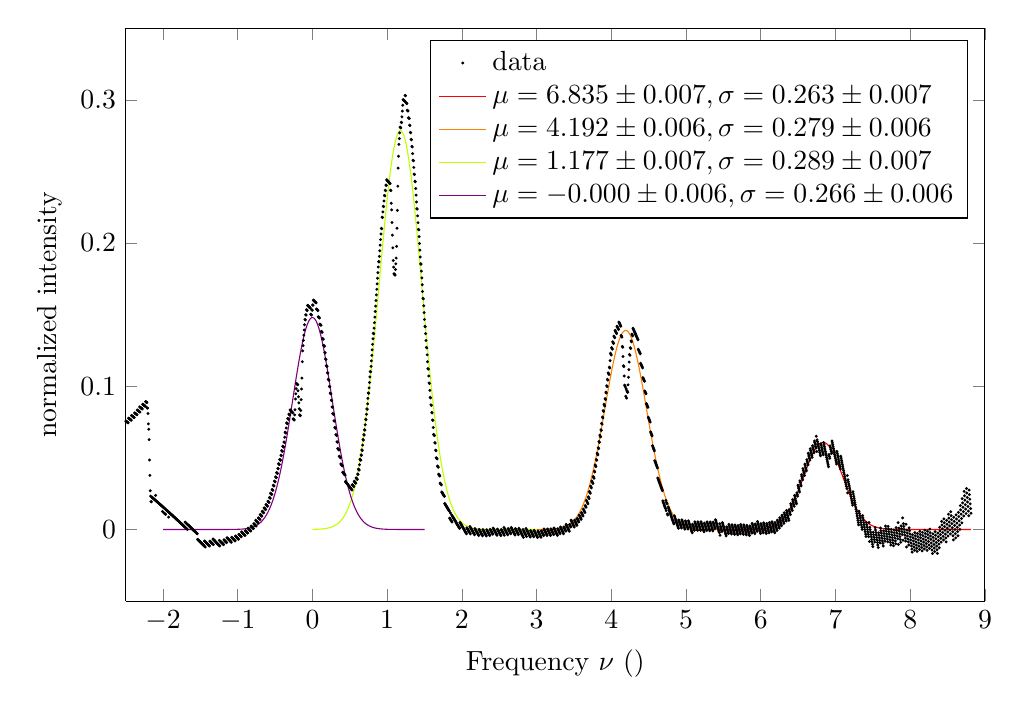
\begin{tikzpicture}

\begin{axis}[%
width=0.9\textwidth,
height=0.6\textwidth,
at={(0\textwidth,0\textwidth)},
scale only axis,
separate axis lines,
xmin=-2.5,
xmax=9,
xlabel={Frequency $\nu ~ (\giga\hertz)$},
ymin=-0.05,
ymax=0.35,
ylabel={normalized intensity},
tick label style={/pgf/number format/fixed},
legend style={legend cell align=left,align=left,draw=black}
]
\addplot [color=black,only marks,mark=*,mark options={solid}, mark size=0.3]
  table[row sep=crcr]{%
-2.640305	0.0710583102080974\\
-2.635194	0.0708568753604485\\
-2.630083	0.0706552219731944\\
-2.624972	0.0704533498186167\\
-2.619861	0.0702512586686124\\
-2.61475	0.0700489482946957\\
-2.609639	0.0698464184679953\\
-2.604528	0.0696436689592553\\
-2.599417	0.069440699538833\\
-2.594306	0.0692375099766992\\
-2.589195	0.0724821218941317\\
-2.584084	0.0722792455441106\\
-2.578973	0.0720761491778654\\
-2.573862	0.0718728325646696\\
-2.568751	0.0716692954734073\\
-2.56364	0.0714655376725728\\
-2.558529	0.0712615589302698\\
-2.553418	0.0710573590142103\\
-2.548307	0.0708529376917141\\
-2.543196	0.0741031337827576\\
-2.538085	0.0738990305270874\\
-2.532974	0.0736947059902552\\
-2.527863	0.0734901599388754\\
-2.522752	0.0732853921391677\\
-2.517641	0.0730804023569563\\
-2.51253	0.0728751903576697\\
-2.507419	0.0761299433843005\\
-2.502308	0.0759250536229427\\
-2.497197	0.0757199417702128\\
-2.492086	0.0755146075908282\\
-2.486975	0.0753090508491074\\
-2.481864	0.0751032713089703\\
-2.476753	0.0748972687339364\\
-2.471642	0.0746910428871241\\
-2.466531	0.0744845935312508\\
-2.46142	0.0777450443221566\\
-2.456309	0.0775389221301604\\
-2.451198	0.0773325765546246\\
-2.446087	0.0771260073575466\\
-2.440976	0.0769192143005201\\
-2.435865	0.0767121971447335\\
-2.430754	0.0765049556509703\\
-2.425643	0.0762974895796067\\
-2.420532	0.0795631453120763\\
-2.415421	0.0793560110039113\\
-2.41031	0.079148652243818\\
-2.405199	0.0789410687914464\\
-2.400088	0.0787332604060373\\
-2.394977	0.0785252268464225\\
-2.389866	0.0783169678710227\\
-2.384755	0.0781084832378477\\
-2.379644	0.0813793962037231\\
-2.374533	0.0811712479676653\\
-2.369422	0.0809628741996727\\
-2.364311	0.0807542746570211\\
-2.3592	0.0805454490965728\\
-2.354089	0.0803363972747746\\
-2.348978	0.0801271189476587\\
-2.343867	0.0834027744243601\\
-2.338756	0.0831938367927023\\
-2.333645	0.082984672782078\\
-2.328534	0.0827752821477795\\
-2.323423	0.0825656646446813\\
-2.318312	0.0823558200272388\\
-2.313201	0.0856356881709729\\
-2.30809	0.0819354484650445\\
-2.302979	0.0852164612513336\\
-2.297868	0.085006507064523\\
-2.292757	0.0847963253975793\\
-2.287646	0.0845859160033714\\
-2.282535	0.0843752786343447\\
-2.277424	0.0841644130425208\\
-2.272313	0.0874496803574375\\
-2.267202	0.0872391641498919\\
-2.262091	0.0870284198469906\\
-2.25698	0.0868174472000044\\
-2.251869	0.0866062459597771\\
-2.246758	0.0863948158767256\\
-2.241647	0.0861831567008382\\
-2.236536	0.085971268181675\\
-2.231425	0.0892619885738503\\
-2.226314	0.0890504542088044\\
-2.221203	0.0888386906281764\\
-2.216092	0.0886266975807675\\
-2.210981	0.0849083766411579\\
-2.20587	0.084695106778953\\
-2.200759	0.0809738724972235\\
-2.195648	0.0737422168485833\\
-2.190537	0.0700164215489968\\
-2.185426	0.0627785576976653\\
-2.180315	0.0485151434484424\\
-2.175204	0.0377567485319665\\
-2.170093	0.0269931719954584\\
-2.164982	0.0232513740735343\\
-2.159871	0.0195076784461581\\
-2.15476	0.0192772175781258\\
-2.149649	0.0225624692686253\\
-2.144538	0.0223323363761682\\
-2.139427	0.0221019540460103\\
-2.134316	0.0218713220020645\\
-2.129205	0.021640439967767\\
-2.124094	0.0214093076660763\\
-2.118983	0.0211779248194722\\
-2.113872	0.0209462911499555\\
-2.108761	0.0207144063790459\\
-2.10365	0.0204822702277818\\
-2.098539	0.0237741634152205\\
-2.093428	0.0200172426659315\\
-2.088317	0.0197843506950061\\
-2.083206	0.019551206223046\\
-2.078095	0.0193178089686676\\
-2.072984	0.0190841586500005\\
-2.067873	0.018850254984685\\
-2.062762	0.0186160976898726\\
-2.057651	0.0183816864822246\\
-2.05254	0.0181470210779109\\
-2.047429	0.0179121011926088\\
-2.042318	0.0176769265415024\\
-2.037207	0.0174414968392821\\
-2.032096	0.0172058118001418\\
-2.026985	0.0169698711377801\\
-2.021874	0.0167336745653978\\
-2.016763	0.0164972217956973\\
-2.011652	0.0162605125408821\\
-2.006541	0.0124840628670163\\
-2.00143	0.0157863234222158\\
-1.996319	0.0155488429802652\\
-1.991208	0.0153111048969981\\
-1.986097	0.0115302063960696\\
-1.980986	0.0148348546447723\\
-1.975875	0.0145963418936781\\
-1.970764	0.0108120939712993\\
-1.965653	0.0105722034941887\\
-1.960542	0.0138792496369955\\
-1.955431	0.013639699907477\\
-1.95032	0.0133998901999568\\
-1.945209	0.0131598202200525\\
-1.940098	0.0129194896728678\\
-1.934987	0.012678898262992\\
-1.929876	0.0124380456944976\\
-1.924765	0.00864368322371356\\
-1.919654	0.0119555558953586\\
-1.914543	0.0117139180702706\\
-1.909432	0.0114720178976744\\
-1.904321	0.0112298550790476\\
-1.89921	0.0109874293153445\\
-1.894099	0.0107447403069965\\
-1.888988	0.0105017877539102\\
-1.883877	0.0102585713554667\\
-1.878766	0.0100150908105202\\
-1.873655	0.00977134581739725\\
-1.868544	0.00952733607389578\\
-1.863433	0.00928306127728351\\
-1.858322	0.00903852112429659\\
-1.853211	0.00879371531113993\\
-1.8481	0.00854864353348461\\
-1.842989	0.00830330548646752\\
-1.837878	0.00805770086468993\\
-1.832767	0.00781182936221647\\
-1.827656	0.00756569067257429\\
-1.822545	0.00731928448875185\\
-1.817434	0.00707261050319685\\
-1.812323	0.00682566840781706\\
-1.807212	0.00657845789397749\\
-1.802101	0.00633097865249954\\
-1.79699	0.00608323037366076\\
-1.791879	0.0058352127471929\\
-1.786768	0.00558692546228079\\
-1.781657	0.00533836820756173\\
-1.776546	0.00508954067112399\\
-1.771435	0.00484044254050553\\
-1.766324	0.00459107350269305\\
-1.761213	0.00434143324412095\\
-1.756102	0.00409152145067004\\
-1.750991	0.00384133780766649\\
-1.74588	0.00359088199988011\\
-1.740769	0.00334015371152441\\
-1.735658	0.00308915262625364\\
-1.730547	0.00283787842716388\\
-1.725436	0.00258633079678949\\
-1.720325	0.00233450941710411\\
-1.715214	0.00208241396951769\\
-1.710103	0.00183004413487642\\
-1.704992	0.0051688477963624\\
-1.699881	0.00132448002498664\\
-1.69477	0.00466455386720122\\
-1.689659	0.00081781452287677\\
-1.684548	0.000564067945827529\\
-1.679437	0.00390605208706452\\
-1.674326	5.5745526922224e-05\\
-1.669215	0.00339900655966618\\
-1.664104	0.00314506952613824\\
-1.658993	0.00289085588132698\\
-1.653882	0.00263636530096512\\
-1.648771	0.00238159746020927\\
-1.64366	0.00212655203363865\\
-1.638549	0.00187122869525302\\
-1.633438	0.00161562711847285\\
-1.628327	0.00135974697613661\\
-1.623216	0.00110358794050058\\
-1.618105	0.000847149683237292\\
-1.612994	0.000590431875434283\\
-1.607883	0.000333434187592574\\
-1.602772	7.61562896263168e-05\\
-1.597661	-0.000181402149139531\\
-1.59255	-0.000439241459970097\\
-1.587439	-0.000697361974721034\\
-1.582328	-0.000955764025841077\\
-1.577217	-0.00121444794637271\\
-1.572106	-0.00147341406995261\\
-1.566995	-0.00173266273081518\\
-1.561884	-0.0019921942637906\\
-1.556773	-0.002252009004309\\
-1.551662	-0.00251210728840023\\
-1.546551	-0.0027724894526957\\
-1.54144	-0.00303315583442898\\
-1.536329	-0.00691610715689395\\
-1.531218	-0.00717828607726267\\
-1.526107	-0.00744075126012045\\
-1.520996	-0.00770350304635059\\
-1.515885	-0.00796654177744771\\
-1.510774	-0.00822986779551904\\
-1.505663	-0.00849348144328554\\
-1.500552	-0.00875738306408369\\
-1.495441	-0.0090215730018659\\
-1.49033	-0.00928605160120322\\
-1.485219	-0.00955081920728507\\
-1.480108	-0.00981587616592172\\
-1.474997	-0.0100812228235454\\
-1.469886	-0.0103468595272112\\
-1.464775	-0.0106127866245984\\
-1.459664	-0.0108790044640132\\
-1.454553	-0.0111455133943879\\
-1.449442	-0.0114123137652835\\
-1.444331	-0.00804027137319729\\
-1.43922	-0.0083066938622991\\
-1.434109	-0.0122144670261637\\
-1.428998	-0.00884041351389264\\
-1.423887	-0.00910771137866173\\
-1.418776	-0.00937530173865397\\
-1.413665	-0.00964318494659433\\
-1.408554	-0.00991136135584547\\
-1.403443	-0.0101798313204082\\
-1.398332	-0.0104485951949234\\
-1.393221	-0.0107176533346729\\
-1.38811	-0.0109870060955815\\
-1.382999	-0.011256653834218\\
-1.377888	-0.0115265969077962\\
-1.372777	-0.00814413951650894\\
-1.367666	-0.00841369767421019\\
-1.362555	-0.00868355117230801\\
-1.357444	-0.00895370036931364\\
-1.352333	-0.00922414562438734\\
-1.347222	-0.00949488729734216\\
-1.342111	-0.00976592574864243\\
-1.337	-0.0100372613394082\\
-1.331889	-0.00664835495883742\\
-1.326778	-0.0105808253870949\\
-1.321667	-0.0071905435022579\\
-1.316556	-0.00746208385574998\\
-1.311445	-0.00773392208099977\\
-1.306334	-0.00800605854176006\\
-1.301223	-0.00827849360244537\\
-1.296112	-0.00855122762813343\\
-1.291001	-0.00882426098456768\\
-1.28589	-0.00909759403815635\\
-1.280779	-0.00937122715597694\\
-1.275668	-0.00964516070577526\\
-1.270557	-0.00991939505596751\\
-1.265446	-0.0101939305756429\\
-1.260335	-0.0104687676345636\\
-1.255224	-0.0107439066031667\\
-1.250113	-0.0110193478525666\\
-1.245002	-0.00761765505726553\\
-1.239891	-0.0115711386816026\\
-1.23478	-0.00816804359229262\\
-1.229669	-0.00844369167470038\\
-1.224558	-0.00871964279768656\\
-1.219447	-0.00899589733509099\\
-1.214336	-0.00927245566143808\\
-1.209225	-0.00954931815193838\\
-1.204114	-0.00982648518248941\\
-1.199003	-0.0101039571296782\\
-1.193892	-0.0103817343707824\\
-1.188781	-0.0106598172837713\\
-1.18367	-0.00724865075005487\\
-1.178559	-0.00752632900702466\\
-1.173448	-0.00780431295421091\\
-1.168337	-0.0080826029709764\\
-1.163226	-0.00836119943738201\\
-1.158115	-0.00864010273418647\\
-1.153004	-0.00891931324284934\\
-1.147893	-0.00919883134553179\\
-1.142782	-0.0057809334052259\\
-1.137671	-0.00606004171176555\\
-1.13256	-0.0063394576321012\\
-1.127449	-0.00661918154980645\\
-1.122338	-0.0068992138491617\\
-1.117227	-0.00717955491515632\\
-1.112116	-0.00746020513348933\\
-1.107005	-0.00774116489057186\\
-1.101894	-0.00802243457352803\\
-1.096783	-0.00830401457019669\\
-1.091672	-0.00858590526913305\\
-1.086561	-0.0088681070596115\\
-1.08145	-0.00544050775687555\\
-1.076339	-0.00572229310281314\\
-1.071228	-0.00600438956440841\\
-1.066117	-0.0062867975323817\\
-1.061006	-0.00656951739817591\\
-1.055895	-0.00685254955395953\\
-1.050784	-0.00713589439262741\\
-1.045673	-0.00741955230780222\\
-1.040562	-0.00770352369383742\\
-1.035451	-0.00798780894581763\\
-1.03034	-0.00455184606671999\\
-1.025229	-0.00483570889496865\\
-1.020118	-0.00511988561625354\\
-1.015007	-0.00540437662713322\\
-1.009896	-0.00568918232490256\\
-1.004785	-0.00597430310759517\\
-0.999674	-0.00625973937398516\\
-0.994563	-0.00654549152358852\\
-0.989452	-0.00683155995666462\\
-0.984341000000001	-0.00338787861098022\\
-0.979229999999999	-0.00367351895474921\\
-0.974119	-0.00395947561136367\\
-0.969008000000001	-0.00424574898258068\\
-0.963897	-0.0045323394709067\\
-0.958786	-0.00481924747959894\\
-0.953675	-0.00510647341266757\\
-0.948564	-0.00165649344560204\\
-0.943453000000001	-0.00194328631980611\\
-0.938342	-0.00223039714855111\\
-0.933231	-0.00251782633736064\\
-0.92812	-0.00280557429251749\\
-0.923009	-0.00309364142106361\\
-0.917898	-0.00338202813080302\\
-0.912787	-0.00367073483030311\\
-0.907676	-0.00395976192889647\\
-0.902565	-0.00424910983668303\\
-0.897454000000001	-0.000790499938543077\\
-0.892342999999999	-0.00107940864301681\\
-0.887232	-0.00136863818994315\\
-0.882121000000001	-0.00165818899096504\\
-0.87701	-0.00194806145849791\\
-0.871899000000001	-0.00223825600573102\\
-0.866788	-0.00252877304663102\\
-0.861677	0.000936265704417627\\
-0.856566	0.000646192930323086\\
-0.851455000000001	0.000355797628499355\\
-0.846344	6.50793834193752e-05\\
-0.841233	-0.000225962221225062\\
-0.836122	-0.000517327602526763\\
-0.831011	-0.00080901717836368\\
-0.8259	-0.00110103136740181\\
-0.820789	0.0023712661424421\\
-0.815678	0.00207970171098337\\
-0.810567000000001	0.00178781263067351\\
-0.805456	0.00149559848126435\\
-0.800345	0.00120305884171479\\
-0.795234	0.000910193290188155\\
-0.790123	0.00061700140405041\\
-0.785012000000001	0.00409584697586907\\
-0.779901	0.00380311000158506\\
-0.77479	0.00351004665624111\\
-0.769679	0.00321665651560366\\
-0.764568000000001	0.00292293915463526\\
-0.759457	0.00640681500299578\\
-0.754346	0.00233452106752985\\
-0.749235000000001	0.00581997168619763\\
-0.744124	0.00552605871721068\\
-0.739013	0.00523181763816005\\
-0.733902	0.00493724802077866\\
-0.728791	0.00464234943598629\\
-0.723680000000001	0.00813287384379635\\
-0.718569	0.00783843982763288\\
-0.713458	0.00754367680765877\\
-0.708347	0.00724858435316622\\
-0.703236	0.00695316203262752\\
-0.698125000000001	0.0104487933472295\\
-0.693014	0.0101538400858527\\
-0.687903	0.00985855692290238\\
-0.682792	0.0095629434252138\\
-0.677681000000001	0.00926699915879659\\
-0.672569999999999	0.0127677707245072\\
-0.667459	0.0124723000410537\\
-0.662348000000001	0.012176498554247\\
-0.657237	0.0118803658284492\\
-0.652126	0.0115839014271913\\
-0.647015	0.0150898468173495\\
-0.641904	0.0147938605565199\\
-0.636793000000001	0.0144975425865392\\
-0.631682	0.0142008924692814\\
-0.626571	0.0139039097657817\\
-0.62146	0.0174150627851298\\
-0.616349	0.0171185628135841\\
-0.611238	0.0168217302230717\\
-0.606127	0.0165245645729617\\
-0.601016	0.0162270654217778\\
-0.595905	0.0197434601088743\\
-0.590794000000001	0.0194464483156349\\
-0.585683	0.0191491029895953\\
-0.580572	0.018851423687603\\
-0.575461000000001	0.0223722682926357\\
-0.57035	0.0220750805953145\\
-0.565239	0.0217775588921753\\
-0.560128	0.0253020476495625\\
-0.555017	0.0250050214082189\\
-0.549906	0.024707661133918\\
-0.544795	0.0244099663809983\\
-0.539684	0.0279389487158692\\
-0.534573	0.0276417537243117\\
-0.529462000000001	0.0273442242289333\\
-0.524351	0.0308768859249744\\
-0.51924	0.0305798600941863\\
-0.514129000000001	0.0302824997371763\\
-0.509018	0.0338188565622692\\
-0.503907000000001	0.0335220037945998\\
-0.498796	0.0332248164811465\\
-0.493685	0.0367648842754003\\
-0.488574	0.0364682084977266\\
-0.483463	0.0361711981575839\\
-0.478352	0.0397149928338174\\
-0.473241	0.0394184979977508\\
-0.46813	0.0391216685854447\\
-0.463019	0.0426692061296751\\
-0.457908	0.0423728962117699\\
-0.452797	0.0459233350332858\\
-0.447686	0.0456275481787402\\
-0.442575000000001	0.0453314271807027\\
-0.437464	0.0488856370249279\\
-0.432353	0.0485900431213067\\
-0.427242	0.048294115070208\\
-0.422131	0.0518521121262358\\
-0.417020000000001	0.0515567152231204\\
-0.411909	0.0551176468375792\\
-0.406798	0.0548227847035825\\
-0.401687	0.0545275888763085\\
-0.396576	0.0580923362134319\\
-0.391465	0.0577976792504455\\
-0.386354	0.0575026886003204\\
-0.381243	0.0610712680560154\\
-0.376132	0.0607768203883509\\
-0.371021	0.0643483681003101\\
-0.36591	0.0679220106139105\\
-0.360799	0.0676289922361419\\
-0.355688000000001	0.0673356415718965\\
-0.350577	0.070913153362069\\
-0.345466	0.0744927719297867\\
-0.340355	0.0742008644226206\\
-0.335244	0.0739086255825793\\
-0.330133000000001	0.0774921384085245\\
-0.325022	0.0772004610772394\\
-0.319911	0.0769084524428298\\
-0.3148	0.0804958762864042\\
-0.309689000000001	0.0802044333997657\\
-0.304577999999999	0.0799126592431786\\
-0.299467	0.0835040109426619\\
-0.294356000000001	0.0832128067969566\\
-0.289245	0.0829212714179486\\
-0.284134	0.0826294043501452\\
-0.279023	0.0823372051371558\\
-0.273912	0.0820446733216911\\
-0.268801000000001	0.0817518084455595\\
-0.26369	0.0814586100496661\\
-0.258579	0.0772717093590699\\
-0.253468	0.076976597344369\\
-0.248357	0.0766811490080994\\
-0.243246	0.0763853638855694\\
-0.238135	0.0799875991419227\\
-0.233024	0.0835919984528083\\
-0.227913	0.0910994264622398\\
-0.222802000000001	0.0947094190716412\\
-0.217691	0.0983215886275711\\
-0.21258	0.101935938966385\\
-0.207469	0.101646589538162\\
-0.202358	0.101356909630945\\
-0.197247	0.101066898785666\\
-0.192136000000001	0.0968668893968786\\
-0.187025	0.0926640205482706\\
-0.181914	0.0884582874434166\\
-0.176803	0.0842496852769264\\
-0.171692	0.0800382092344225\\
-0.166581	0.0797398551090754\\
-0.16147	0.0794411595418429\\
-0.156359	0.0830606662176315\\
-0.151248	0.0906021965297646\\
-0.146137	0.0981484870904653\\
-0.141026	0.105699546188843\\
-0.135915	0.117179030881049\\
-0.130804	0.124740931789113\\
-0.125693	0.128381417832384\\
-0.120582	0.132024141709718\\
-0.115471	0.13566910737565\\
-0.11036	0.139316318792057\\
-0.105249	0.142965779928174\\
-0.100138	0.146617494760614\\
-0.0950270000000004	0.146337538881132\\
-0.0899160000000001	0.149992481464688\\
-0.0848050000000002	0.149713175157083\\
-0.0796939999999999	0.153371355547848\\
-0.0745830000000001	0.153092702946125\\
-0.0694720000000002	0.152813729978839\\
-0.0643610000000003	0.156476136490808\\
-0.05925	0.156197821970765\\
-0.0541390000000002	0.15591918722296\\
-0.0490279999999998	0.155640231794826\\
-0.043917	0.155360955232882\\
-0.0388060000000001	0.155081357082739\\
-0.0336950000000003	0.154801436889091\\
-0.0285840000000004	0.154521194195717\\
-0.0234730000000001	0.150288481949896\\
-0.0183620000000002	0.150006280319004\\
-0.0132509999999999	0.149723753300771\\
-0.00814000000000048	0.153396989268334\\
-0.00302900000000017	0.153115127200776\\
0.0020819999999997	0.156791664456807\\
0.007193	0.156510471568104\\
0.0123039999999999	0.160190320433906\\
0.0174150000000002	0.159909800970733\\
0.0225259999999996	0.159628957451845\\
0.0276369999999999	0.159347789415149\\
0.0327479999999998	0.159066296397617\\
0.0378590000000001	0.158784477935283\\
0.04297	0.158502333563241\\
0.0480810000000003	0.158219862815643\\
0.0531919999999997	0.153965070250346\\
0.0583029999999996	0.1536806098555\\
0.0634139999999999	0.153395820135753\\
0.0685249999999997	0.153110700619247\\
0.073636	0.15282525083317\\
0.0787469999999999	0.148560782370902\\
0.0838579999999998	0.148273327375755\\
0.0889689999999996	0.147985539129573\\
0.0940799999999999	0.147697417153449\\
0.0991909999999998	0.143424890691643\\
0.104302	0.143134750324923\\
0.109413	0.142844273219446\\
0.114524	0.142553458890131\\
0.119635	0.138272829208356\\
0.124746	0.137979983203627\\
0.129857	0.137686796938596\\
0.134968	0.133399720245649\\
0.140079	0.133104491483823\\
0.145189999999999	0.132808919402582\\
0.150301	0.128515367576746\\
0.155412	0.128217742111329\\
0.160523	0.127919770244545\\
0.165634	0.123619715013274\\
0.170745	0.123319678808414\\
0.175856	0.119014814983487\\
0.180967	0.118712706036022\\
0.186078	0.114403018806548\\
0.191189	0.114098828675809\\
0.1963	0.113794283792409\\
0.201411	0.109478023385068\\
0.206522	0.109171386197923\\
0.211633	0.10485026672948\\
0.216744	0.104541528711406\\
0.221855	0.104232430114861\\
0.226966	0.0999046877696474\\
0.232077	0.0995934771028094\\
0.237188	0.0952608397166821\\
0.242299	0.0949475083647171\\
0.24741	0.094633810534271\\
0.252521	0.0902945001140988\\
0.257632	0.0899786702386705\\
0.262743	0.0856344284705569\\
0.267854	0.085316457846505\\
0.272965	0.0809672694592973\\
0.278076	0.0806471493452068\\
0.283187	0.0803266540367946\\
0.288298	0.0759707206271175\\
0.293409	0.075648064294491\\
0.29852	0.071287147489\\
0.303631	0.0709623213002698\\
0.308742	0.0706371138322702\\
0.313853	0.0662694007163419\\
0.318964	0.0659420117336024\\
0.324075	0.0656142381162923\\
0.329186	0.0612396986870958\\
0.334297	0.0609097318238742\\
0.339408	0.0565301501219163\\
0.344519	0.0561979810356094\\
0.34963	0.0558654211069683\\
0.354741	0.0555324697568739\\
0.359852	0.051144187033346\\
0.364963	0.0508090187550824\\
0.370074	0.0504734556233405\\
0.375185	0.0501374970516458\\
0.380296	0.0457404635738896\\
0.385407	0.0454022732502014\\
0.390518	0.0450636840223084\\
0.395629	0.0447246952962893\\
0.40074	0.0443853064769791\\
0.405851	0.03997762555081\\
0.410962	0.0396359871340259\\
0.416073	0.0392939451208123\\
0.421184	0.0389514989084462\\
0.426295	0.0386086478929397\\
0.431406	0.038265391469038\\
0.436517	0.037921729030214\\
0.441628	0.0334995992058224\\
0.446739	0.0331536632671633\\
0.45185	0.0328073177581983\\
0.456961	0.0324605620646921\\
0.462072	0.0321133955711158\\
0.467183	0.0317658176606446\\
0.472294	0.0314178277151533\\
0.477405	0.0310694251152142\\
0.482516	0.0307206092400922\\
0.487627	0.0303713794677434\\
0.492738	0.0300217351748093\\
0.497849	0.0296716757366158\\
0.50296	0.0293212005271676\\
0.508071	0.0289703089191463\\
0.513182	0.0286190002839066\\
0.518293	0.0282672739914723\\
0.523404	0.0279151294105333\\
0.528515	0.0275625659084422\\
0.533626	0.03131418376745\\
0.538737	0.0309622716726886\\
0.543848	0.0306099405264145\\
0.548959	0.0302571896932876\\
0.55407	0.0299040185366182\\
0.559181	0.0336625008826927\\
0.564292	0.0333099872215868\\
0.569403	0.0329570531078984\\
0.574514	0.0326036979022259\\
0.579625	0.0322499209638063\\
0.584736	0.0360153143243401\\
0.589847	0.0356622010238744\\
0.594958	0.0353086658629922\\
0.600069	0.0349547081982003\\
0.60518	0.0387259670111925\\
0.610291	0.0383726786616132\\
0.615402	0.0421476416416865\\
0.620513	0.0417950272777944\\
0.625624	0.0414419908106712\\
0.630735	0.0452217706820561\\
0.635846	0.0490041778685781\\
0.640957	0.0486529255766753\\
0.646068	0.0483012522495329\\
0.651179	0.0520885087312527\\
0.65629	0.051737524077858\\
0.661401	0.0555285369830768\\
0.666512	0.0551782457694998\\
0.671623	0.0589730272374885\\
0.676734	0.0627704675819242\\
0.681845	0.0624219964682491\\
0.686956	0.0662232255217007\\
0.692067	0.0658754617179095\\
0.697178	0.0696804917397493\\
0.702289	0.069333440098183\\
0.7074	0.0731422833939741\\
0.712511	0.076953814490812\\
0.717622	0.0766086177120533\\
0.722733	0.0804239825002349\\
0.727844	0.0842420481366515\\
0.732955	0.0838987228992283\\
0.738066	0.0877206427670811\\
0.743177	0.0915452766050237\\
0.748288	0.0953726294330132\\
0.753399	0.0950323484400545\\
0.75851	0.0988635843404021\\
0.763621	0.10269755245605\\
0.768732	0.106534257845521\\
0.773843	0.110373705577785\\
0.778954	0.110037673848943\\
0.784065	0.113881041993259\\
0.789176	0.117727165838638\\
0.794287	0.121576050493126\\
0.799398	0.125427701075346\\
0.804509	0.129282122714533\\
0.80962	0.133139320550559\\
0.814731	0.136999299733962\\
0.819842	0.136671148671959\\
0.824953	0.140535111145621\\
0.830064	0.144401868546935\\
0.835175	0.148271426066363\\
0.840286	0.152143788905175\\
0.845397	0.156018962275478\\
0.850508	0.159896951400244\\
0.855619	0.163777761513343\\
0.86073	0.167661397859568\\
0.865841	0.17154786569467\\
0.870952	0.175437170285385\\
0.876063	0.179329316909466\\
0.881174	0.18322431085571\\
0.886285	0.187122157423992\\
0.891396	0.186809439331156\\
0.896507	0.190711384810962\\
0.901618	0.194616196900433\\
0.906729	0.198523880940924\\
0.91184	0.202434442285015\\
0.916951	0.206347886296537\\
0.922062	0.210264218350606\\
0.927173	0.209958623639215\\
0.932284	0.218105568143469\\
0.937395	0.217802502105991\\
0.942506	0.221728800109408\\
0.947617	0.225658011194131\\
0.952728	0.225357119596056\\
0.957839	0.229290526945786\\
0.96295	0.233226861715419\\
0.968061	0.232928163428711\\
0.973172	0.236868717174716\\
0.978283	0.236570940209552\\
0.983394	0.240515726799112\\
0.988505	0.240218876937513\\
0.993616	0.244167910292221\\
0.998727	0.243871993344815\\
1.003838	0.243575712793738\\
1.008949	0.243279068056463\\
1.01406	0.242982058549169\\
1.019171	0.242684683686734\\
1.024282	0.242386942882736\\
1.029393	0.242088835549447\\
1.034504	0.241790361097828\\
1.039615	0.24149151893753\\
1.044726	0.236929343917765\\
1.049837	0.236628081533706\\
1.054948	0.227793782196131\\
1.060059	0.223220381836287\\
1.06517	0.214373516866414\\
1.070281	0.205519506861527\\
1.075392	0.196658338673288\\
1.080503	0.187789999124975\\
1.085614	0.18319096212072\\
1.090725	0.178588126778244\\
1.095836	0.178261374816293\\
1.100947	0.177934218471467\\
1.106058	0.177606657088213\\
1.111169	0.181563696832373\\
1.11628	0.185523750779169\\
1.121391	0.189486824628212\\
1.126502	0.1977430681122\\
1.131613	0.210297636900066\\
1.136724	0.222862120006968\\
1.141835	0.239731836347148\\
1.146946	0.252317926845553\\
1.152057	0.260615240989484\\
1.157168	0.268919091388839\\
1.162279	0.272927284905744\\
1.16739	0.276938575992726\\
1.172501	0.280952970516117\\
1.177612	0.280663067574001\\
1.182723	0.280372803624262\\
1.187834	0.284393063237009\\
1.192945	0.284103817938899\\
1.198056	0.288128584244867\\
1.203167	0.292156482926336\\
1.208278	0.296187519928888\\
1.213389	0.300221701211081\\
1.2185	0.299937660277057\\
1.223611	0.299653264520127\\
1.228722	0.299368513356385\\
1.233833	0.299083406200596\\
1.238944	0.303126350228746\\
1.244055	0.302842293654371\\
1.249166	0.298225942908584\\
1.254277	0.297939405905553\\
1.259388	0.297652509964242\\
1.264499	0.297365254491369\\
1.26961	0.292738611971877\\
1.274721	0.292448858018993\\
1.279832	0.292158740516186\\
1.284943	0.28752389235098\\
1.290054	0.287231261605875\\
1.295165	0.286938263257964\\
1.300276	0.282295170457308\\
1.305387	0.281999644002097\\
1.310498	0.277350435225172\\
1.315609	0.277052369192122\\
1.32072	0.272397023922081\\
1.325831	0.272096406784318\\
1.330942	0.267434904417764\\
1.336053	0.267131724591736\\
1.341164	0.262464044438243\\
1.346275	0.257792363006949\\
1.351386	0.257484411565005\\
1.356497	0.252806518862095\\
1.361608	0.248124604656596\\
1.366719	0.247811848341873\\
1.37183	0.243123689158552\\
1.376941	0.242808318647432\\
1.382052	0.238113893427468\\
1.387163	0.23341541348084\\
1.392274	0.228712871195557\\
1.397385	0.224006258942521\\
1.402496	0.223681549024499\\
1.407607	0.218968610724678\\
1.412718	0.214251581795973\\
1.417829	0.209530454544303\\
1.42294	0.209198562577256\\
1.428051	0.204471061713316\\
1.433162	0.199739441684924\\
1.438273	0.195003694732283\\
1.443384	0.19026381307806\\
1.448495	0.185519788927333\\
1.453606	0.185176068153203\\
1.458717	0.180425595869147\\
1.463828	0.175670959966711\\
1.468939	0.170912152584128\\
1.47405	0.166149165841793\\
1.479161	0.161381991842216\\
1.484272	0.161026273860178\\
1.489383	0.156252576170837\\
1.494494	0.151474669817094\\
1.499605	0.146692546833457\\
1.504716	0.141906199236293\\
1.509827	0.141540667131346\\
1.514938	0.136747732879016\\
1.520049	0.131950552366503\\
1.52516	0.127149117541197\\
1.530271	0.126776029320315\\
1.535382	0.121967957912799\\
1.540493	0.117155610354217\\
1.545604	0.112338978522204\\
1.550715	0.11195826296098\\
1.555826	0.107134944160994\\
1.560937	0.102307319055475\\
1.566048	0.101921313542874\\
1.571159	0.0970869646023531\\
1.57627	0.0922482871805143\\
1.581381	0.0918569546270172\\
1.586492	0.08701151625243\\
1.591603	0.0866172526725466\\
1.596714	0.081765030109224\\
1.601825	0.0813678221135122\\
1.606936	0.0765087920237851\\
1.612047	0.0761086261549792\\
1.617158	0.0712427650989133\\
1.622269	0.0663725106576156\\
1.62738	0.0659669122663138\\
1.632491	0.065560790006118\\
1.637602	0.0606811962855807\\
1.642713	0.0602720753693213\\
1.647824	0.0553855797431756\\
1.652935	0.0549734464380447\\
1.658046	0.0500800250513973\\
1.663157	0.0496648655546228\\
1.668268	0.0492491681823348\\
1.673379	0.0443462948857545\\
1.67849	0.0439275530292982\\
1.683601	0.0435082679335023\\
1.688712	0.0385958961100932\\
1.693823	0.0381735481043461\\
1.698934	0.0377506514484784\\
1.704045	0.0373272051844682\\
1.709156	0.0324027560545778\\
1.714267	0.0319762238201716\\
1.719378	0.0315491365080015\\
1.724489	0.031121493146304\\
1.7296	0.0261848894714977\\
1.734711	0.0257541368610643\\
1.739822	0.0253228226718816\\
1.744933	0.0248909459182458\\
1.750044	0.0244585056120815\\
1.755155	0.0240255007629333\\
1.760266	0.023591930377959\\
1.765377	0.0231577934619223\\
1.770488	0.0181986588737474\\
1.775599	0.017761370747612\\
1.78071	0.0173235104535524\\
1.785821	0.016885076982033\\
1.790932	0.0164460693210768\\
1.796043	0.0160064864562585\\
1.801154	0.0155663273706964\\
1.806265	0.0151255910450455\\
1.811376	0.0146842764574907\\
1.816487	0.0142423825837382\\
1.821598	0.0137999083970086\\
1.826709	0.0133568528680295\\
1.83182	0.0129132149650278\\
1.836931	0.00791815952309427\\
1.842042	0.00747130397057538\\
1.847153	0.0115787966564884\\
1.852264	0.00657582727136685\\
1.857375	0.00612720402882183\\
1.862486	0.0102390995962635\\
1.867597	0.00522818249903712\\
1.872708	0.00934302163221945\\
1.877819	0.00889409551686304\\
1.88293	0.00844457657054398\\
1.888041	0.00799446373347812\\
1.893152	0.00754375594328782\\
1.898263	0.00709245213499499\\
1.903374	0.00664055124101237\\
1.908485	0.00618805219113594\\
1.913596	0.0057349539125372\\
1.918707	0.00528125532975454\\
1.923818	0.00482695536468591\\
1.928929	0.00437205293658005\\
1.93404	0.00391654696202892\\
1.939151	0.00346043635495974\\
1.944262	0.00300372002662597\\
1.949373	0.00254639688559999\\
1.954484	0.0020884658377649\\
1.959595	0.00162992578630539\\
1.964706	0.00117077563170065\\
1.969817	0.000711014271714716\\
1.974928	0.00485778050645225\\
1.980039	0.00439891778256118\\
1.98515	0.00393944336214125\\
1.990261	0.00347935613714556\\
1.995372	0.00301865499678355\\
2.000483	0.00255733882751297\\
2.005594	0.00209540651303053\\
2.010705	0.00163285693426396\\
2.015816	0.00116968896936342\\
2.020927	0.000705901493693095\\
2.026038	0.000241493379821933\\
2.031149	-0.000223536502483856\\
2.03626	-0.000689189286271041\\
2.041371	-0.00115546610740647\\
2.046482	-0.00162236810458682\\
2.051593	-0.0020898964193472\\
2.056704	-0.0025580521960693\\
2.061815	-0.00302683658199099\\
2.066926	0.00114956524837406\\
2.072037	0.000681696325396386\\
2.077148	0.000213198260522462\\
2.082259	-0.00025593009963365\\
2.08737	-0.000725689911345251\\
2.092481	-0.00119608233378132\\
2.097592	-0.0016671085290163\\
2.102703	-0.00213876966203919\\
2.107814	0.00205224038714935\\
2.112925	-0.00308400141602605\\
2.118036	0.0011101352666657\\
2.123147	0.000638128313971031\\
2.128258	0.000165483535010669\\
2.133369	-0.000307800247380641\\
2.13848	-0.000781724213332335\\
2.143591	-0.00125628954594825\\
2.148702	-0.00173149743131562\\
2.153813	-0.0022073490585135\\
2.158924	-0.00268384561962387\\
2.164035	-0.00316098830973988\\
2.169146	-0.00363877832697579\\
2.174257	0.0005749196549657\\
2.179368	9.80701072876844e-05\\
2.184479	-0.000379427338299099\\
2.18959	-0.000857573886432039\\
2.194701	-0.00133637074480331\\
2.199812	-0.00181581912416906\\
2.204923	-0.00229592023835945\\
2.210034	-0.00277667530428793\\
2.215145	-0.00325808554196083\\
2.220256	-0.0037401521744882\\
2.225367	-0.00422287642809205\\
2.230478	1.06712638071604e-05\\
2.235589	-0.000471099419893539\\
2.2407	-0.000953528317332308\\
2.245811	-0.00143661666146655\\
2.250922	-0.00192036568840037\\
2.256033	-0.0024047766373958\\
2.261144	-0.00288985075088322\\
2.266255	-0.00337558927447001\\
2.271366	-0.00386199345695171\\
2.276477	-0.00434906455032169\\
2.281588	-9.70075653961011e-05\\
2.286699	-0.000583112434819455\\
2.29181	-0.00106988482678827\\
2.296921	-0.00155732600022396\\
2.302032	-0.00204543721728156\\
2.307143	-0.00253421974336154\\
2.312254	-0.00302367484711863\\
2.317365	-0.00351380380047206\\
2.322476	-0.00400460787861823\\
2.327587	-0.00449608836003823\\
2.332698	-0.000225269054821009\\
2.337809	-0.000715770470404609\\
2.34292	-0.00120694892055595\\
2.348031	-0.00169880569088443\\
2.353142	-0.00219134207032434\\
2.358253	-0.00268455935114287\\
2.363364	-0.00317845882895296\\
2.368475	-0.00367304180272265\\
2.373586	-0.00416830957478642\\
2.378697	0.000119852089385586\\
2.383808	-0.000374424241271321\\
2.388919	-0.000869386017888107\\
2.39403	-0.00136503455010883\\
2.399141	-0.00186137115098139\\
2.404252	-0.00235839713696961\\
2.409363	-0.00285611382796525\\
2.414474	-0.00335452254729707\\
2.419585	0.000949502768790689\\
2.424696	0.000452097381046457\\
2.429807	-4.6000695527626e-05\\
2.434918	-0.000544792791726811\\
2.440029	-0.00104428024182424\\
2.44514	-0.00154446438358202\\
2.450251	-0.00204534655826216\\
2.455362	-0.00254692811063895\\
2.460473	-0.00304921038900896\\
2.465584	-0.00355219474520374\\
2.470695	-0.00405588253460154\\
2.475806	0.000269341591152217\\
2.480917	-0.000233328785717468\\
2.486028	-0.000736703281773554\\
2.491139	-0.00124078326010979\\
2.49625	-0.00174557008740628\\
2.501361	-0.00225106513394335\\
2.506472	-0.00275726977361113\\
2.511583	-0.00326418538392215\\
2.516694	-0.00377181334602406\\
2.521805	-0.00428015504471113\\
2.526916	6.48422951807781e-05\\
2.532027	-0.000442468372558347\\
2.537138	-0.000950493485083692\\
2.542249	-0.00145923443513474\\
2.54736	-0.0019686926191389\\
2.552471	-0.00247886943722553\\
2.557582	-0.00298976629323722\\
2.562693	0.00136998134989286\\
2.567804	-0.00401372575304548\\
2.572915	0.00034955246331636\\
2.578026	-0.000161744525861929\\
2.583137	-0.000673765098632373\\
2.588248	-0.00118651067445263\\
2.593359	-0.00169998267656202\\
2.59847	-0.00221418253199457\\
2.603581	-0.0027291116715904\\
2.608692	-0.00324477153001013\\
2.613803	-0.00376116354574618\\
2.618914	0.000620629322576338\\
2.624025	0.0001052948109036\\
2.629136	-0.000410772604021892\\
2.634247	-0.000927574369057549\\
2.639358	-0.0014451119349379\\
2.644469	-0.00196338675628915\\
2.64958	-0.00248240029163993\\
2.654691	-0.00300215400343551\\
2.659802	0.00139657931527204\\
2.664913	0.000877895938045992\\
2.670024	0.000358471623345458\\
2.675135	-0.00016169509982622\\
2.680246	-0.000682605706429751\\
2.685357	-0.00120426167540111\\
2.690468	-0.00172666448966718\\
2.695579	-0.00224981563615745\\
2.70069	-0.00277371660581771\\
2.705801	-0.003298368893625\\
2.710912	-0.00382377399859912\\
2.716023	0.000597603194033902\\
2.721134	7.32835830614675e-05\\
2.726245	-0.000451789635804944\\
2.731356	-0.000977617970432387\\
2.736467	-0.00150420293278075\\
2.741578	-0.00203154603891464\\
2.746689	-0.00255964880901982\\
2.7518	-0.00308851276741584\\
2.756911	-0.00361813944256939\\
2.762022	0.000822501961440403\\
2.767133	0.000293974739375424\\
2.772244	-0.000235316011227393\\
2.777355	-0.000765371827918582\\
2.782466	-0.00129619425244609\\
2.787577	-0.0018277848307704\\
2.792688	-0.00236014511307925\\
2.797799	-0.00289327665380013\\
2.80291	-0.00342718101161621\\
2.808021	-0.00396185974948127\\
2.813132	-0.00449731443463297\\
2.818243	-3.3379739909023e-05\\
2.823354	-0.00557055793725847\\
2.828465	-0.0011028357321019\\
2.833576	-0.00163873049118757\\
2.838687	-0.00217540519878856\\
2.843798	-0.00271286144023275\\
2.848909	-0.00325110080521496\\
2.85402	-0.00379012488781028\\
2.859131	0.000691714389941311\\
2.864242	-0.00487053360414125\\
2.869353	-0.000384861840830864\\
2.874464	-0.000924329927883383\\
2.879575	-0.00146458680540706\\
2.884686	-0.00200563408598087\\
2.889797	-0.00254747338664973\\
2.894908	-0.00309010632893991\\
2.900019	-0.00363353453887338\\
2.90513	-0.00417775964698497\\
2.910241	-0.00472278328833742\\
2.915352	-0.00526860710253607\\
2.920463	-0.000760884830561359\\
2.925574	-0.00130556302753804\\
2.930685	-0.00185104229777222\\
2.935796	-0.00239732429087014\\
2.940907	-0.00294441066103723\\
2.946018	-0.00349230306709547\\
2.951129	-0.00404100317249689\\
2.95624	-0.00459051264534271\\
2.961351	-0.00514083315839731\\
2.966462	-0.000612714033604966\\
2.971573	-0.00116187404981205\\
2.976684	-0.00171184603101815\\
2.981795	-0.00226263166026364\\
2.986906	-0.00281423262531022\\
2.992017	-0.00336665061865848\\
2.997128	-0.0039198873375641\\
3.002239	-0.00447394448405403\\
3.00735	-0.00502882376494451\\
3.012461	-0.00558452689185618\\
3.017572	-0.00103374057828165\\
3.022683	-0.00158826733326611\\
3.027794	-0.00214361888996306\\
3.032905	-0.00269979697059708\\
3.038016	-0.00325680330225797\\
3.043127	-0.0038146396169183\\
3.048238	-0.00437330765145072\\
3.053349	-0.00493280914764438\\
3.05846	-0.00549314585222338\\
3.063571	-0.000921389315247323\\
3.068682	-0.00148053428648565\\
3.073793	-0.00204051544790862\\
3.078904	-0.00260133455713962\\
3.084015	-0.00316299337679937\\
3.089126	-0.00372549367452235\\
3.094237	-0.00428883722297613\\
3.099348	0.000300066640121055\\
3.104459	-0.000262071130639807\\
3.10957	-0.000825053148715948\\
3.114681	-0.00138888119788838\\
3.119792	-0.00195355706703459\\
3.124903	-0.00251908255014643\\
3.130014	-0.00308545944634786\\
3.135125	-0.00365268955991382\\
3.140236	-0.00422077470028914\\
3.145347	0.00038961175440011\\
3.150458	-0.000177251771979137\\
3.155569	-0.000744971349204704\\
3.16068	-0.00131354879814904\\
3.165791	-0.00188298594491965\\
3.170902	-0.0024532846208789\\
3.176013	-0.003024446662661\\
3.181124	-0.00359647391219275\\
3.186235	-0.0041693682167121\\
3.191346	0.000462791531984807\\
3.196457	-0.000108865067439012\\
3.201568	-0.00068138977422727\\
3.206679	-0.0012547844473707\\
3.21179	-0.00182905095123953\\
3.216901	-0.00240419115560275\\
3.222012	-0.00298020693564682\\
3.227123	-0.00355710017199695\\
3.232234	0.00109499637817501\\
3.237345	0.000519356387430614\\
3.242456	-5.71621346767692e-05\\
3.247567	-0.000634561080811613\\
3.252678	-0.00121284234914576\\
3.257789	-0.00179200784337996\\
3.2629	-0.00237205947276298\\
3.268011	-0.002952999152112\\
3.273122	-0.00353482880183242\\
3.278233	-0.00411755034793937\\
3.283344	0.000559049805263445\\
3.288455	-2.24010664537921e-05\\
3.293566	-0.000604744946417934\\
3.298677	-0.00118798377308282\\
3.303788	-0.00177211949058487\\
3.308899	-0.00235715404876302\\
3.31401	-0.00294308940318078\\
3.319121	0.00175180894546023\\
3.324232	0.00116715949222401\\
3.329343	0.000581608113597309\\
3.334454	-4.84715867532515e-06\\
3.339565	-0.000592208298648256\\
3.344676	-0.00118047728619586\\
3.349787	-0.00176965610703528\\
3.354898	-0.00235974675274542\\
3.360009	-0.00295075122079114\\
3.36512	0.00176707807018939\\
3.370231	0.00117737665110673\\
3.375342	0.00058676024870119\\
3.380453	-4.77314755542579e-06\\
3.385564	-0.000597225554152869\\
3.390675	-0.00119059899356633\\
3.395786	0.00354374756686193\\
3.400897	0.00295169204266432\\
3.406008	0.00235871431367207\\
3.411119	0.00176481234413528\\
3.41623	0.00116998409224001\\
3.421341	0.000574227510085845\\
3.426452	-2.2459456337387e-05\\
3.431563	-0.000620078867171747\\
3.436674	-0.00121863278871381\\
3.441785	0.00353919287390625\\
3.446896	0.00294197455848189\\
3.452007	0.00234382052703108\\
3.457118	0.00174472869958997\\
3.462229	0.00651488679108603\\
3.46734	0.00591714414811217\\
3.472451	0.00531846250740231\\
3.477562	0.00471883977522025\\
3.482673	0.00411827385153307\\
3.487784	0.00351676262998735\\
3.492895	0.00291430399788484\\
3.498006	0.00231089583615851\\
3.503117	0.00170653601935011\\
3.508228	0.00650067526739195\\
3.513339	0.00589768287094194\\
3.51845	0.00529373758319496\\
3.523561	0.00468883726450942\\
3.528672	0.00408297976876537\\
3.533783	0.00347616294333952\\
3.538894	0.00286838462908146\\
3.544005	0.0076821446023515\\
3.549116	0.00707575043606601\\
3.554227	0.00646839352498296\\
3.559338	0.00586007169547065\\
3.564449	0.00525078276728086\\
3.56956	0.0100796473701716\\
3.574671	0.00947175773025921\\
3.579782	0.00886289973162824\\
3.584893	0.00825307117937402\\
3.590004	0.00764226987188443\\
3.595115	0.00703049360081642\\
3.600226	0.0118769833370521\\
3.605337	0.0112666226452594\\
3.610448	0.0106552857177773\\
3.615559	0.0100429703313598\\
3.62067	0.00942967425593821\\
3.625781	0.0142915532918603\\
3.630892	0.01367968837036\\
3.636003	0.0130668414838041\\
3.641114	0.0124530103870386\\
3.646225	0.0118381928279926\\
3.651336	0.0167155955112746\\
3.656447	0.0161022248951376\\
3.661558	0.0154878665368481\\
3.666669	0.0203760236541539\\
3.67178	0.0197631262463877\\
3.676891	0.0191492398296117\\
3.682002	0.0185343621281513\\
3.687113	0.0179184908592769\\
3.692224	0.022822401127935\\
3.697335	0.0222080070009502\\
3.702446	0.021592618036315\\
3.707557	0.0265074396649687\\
3.712668	0.0258935421770787\\
3.717779	0.0252786485949705\\
3.72289	0.0302044454948611\\
3.728001	0.0295910578692593\\
3.733112	0.0289766729068853\\
3.738223	0.0339135095023871\\
3.743334	0.0333006451229823\\
3.748445	0.0326867821786161\\
3.753556	0.032071918345736\\
3.758667	0.037022395826303\\
3.763778	0.036409068461465\\
3.768889	0.0357947389861977\\
3.774	0.04075640271978\\
3.779111	0.0401436246614495\\
3.784222	0.0451139721039647\\
3.789333	0.0445027594065507\\
3.794444	0.0438905445494147\\
3.799555	0.0488721946270159\\
3.804666	0.048261560362551\\
3.809777	0.0532519820491019\\
3.814888	0.05264294255764\\
3.819999	0.0520329009468818\\
3.82511	0.0570347432912605\\
3.830221	0.056426311974348\\
3.835332	0.0614370150467708\\
3.840443	0.0608302084453189\\
3.845554	0.0658498106369042\\
3.850665	0.0652446432817553\\
3.855776	0.0646384752258222\\
3.860887	0.0696696697385735\\
3.865998	0.0690651568823686\\
3.871109	0.074105341406301\\
3.87622	0.0735024985292393\\
3.881331	0.078551712213757\\
3.886442	0.0779505542077015\\
3.891553	0.0830088364307595\\
3.896664	0.0824093783010139\\
3.901775	0.0874767686708571\\
3.906886	0.08687902553717\\
3.911997	0.0862802861684252\\
3.917108	0.0913595509916657\\
3.922219	0.0907625433054208\\
3.92733	0.0958510100902961\\
3.932441	0.0952557494671232\\
3.937552	0.100353458611977\\
3.942663	0.0997599605502958\\
3.947774	0.104866952691596\\
3.952885	0.104275232808722\\
3.957996	0.109391548822888\\
3.963107	0.108801622856092\\
3.968218	0.108210705821738\\
3.973329	0.113339187668924\\
3.97844	0.11275008200783\\
3.983551	0.117887984589501\\
3.988662	0.12303251990809\\
3.993773	0.122448071328851\\
3.998884	0.121862636570982\\
4.003995	0.127019505969746\\
4.009106	0.126435930990053\\
4.014217	0.125851369135095\\
4.019328	0.131020648153259\\
4.024439	0.130437964185291\\
4.02955	0.129854292669718\\
4.034661	0.135036057486022\\
4.039772	0.134454282157723\\
4.044883	0.13387151863431\\
4.049994	0.13906584607418\\
4.055105	0.138484997232278\\
4.060216	0.137903159573124\\
4.065327	0.137320330677541\\
4.070438	0.136736508118394\\
4.075549	0.141949329128608\\
4.08066	0.141367443587992\\
4.085771	0.140784563772405\\
4.090882	0.140200687239057\\
4.095993	0.139615811537089\\
4.101104	0.144847299516946\\
4.106215	0.144264383507744\\
4.111326	0.143680467729744\\
4.116437	0.143095549716257\\
4.121548	0.142509626992412\\
4.126659	0.141922697075124\\
4.13177	0.135493497319812\\
4.136881	0.13490053905861\\
4.141992	0.134306559202405\\
4.147103	0.127858254915208\\
4.152214	0.127258197026178\\
4.157325	0.120795741237279\\
4.162436	0.1143241643778\\
4.167547	0.113712893930084\\
4.172658	0.107227059352377\\
4.177769	0.100732039838966\\
4.18288	0.100109449207243\\
4.187991	0.0994857785788759\\
4.193102	0.0929712280344234\\
4.198213	0.0982351865276035\\
4.203324	0.0917102744488468\\
4.208435	0.096980241985074\\
4.213546	0.0963511307083611\\
4.218657	0.0957209231049748\\
4.223768	0.10100406337257\\
4.228879	0.106294368574654\\
4.23399	0.111591857597897\\
4.239101	0.116896549392323\\
4.244212	0.122208462971581\\
4.249323	0.12159243113711\\
4.254434	0.126914675912744\\
4.259545	0.126300659659865\\
4.264656	0.13163328317475\\
4.269767	0.131021300912086\\
4.274878	0.136364351005209\\
4.279989	0.135754421290244\\
4.2851	0.135143417947008\\
4.290211	0.140500087639579\\
4.295322	0.139891157529871\\
4.300433	0.139281153042947\\
4.305544	0.138670071442456\\
4.310655	0.138057909982688\\
4.315766	0.137444665908531\\
4.320877	0.136830336455432\\
4.325988	0.136214918849357\\
4.331099	0.135598410306746\\
4.33621	0.13498080803448\\
4.341321	0.134362109229832\\
4.346432	0.133742311080433\\
4.351543	0.133121410764222\\
4.356654	0.132499405449414\\
4.361765	0.125847655435383\\
4.366876	0.125219096701069\\
4.371987	0.124589416680997\\
4.377098	0.123958612484104\\
4.382209	0.123326681209318\\
4.38732	0.122693619945514\\
4.392431	0.116004663190583\\
4.397542	0.115364951588622\\
4.402653	0.114724093349836\\
4.407764	0.114082085502093\\
4.412875	0.113438925062918\\
4.417986	0.112794609039445\\
4.423097	0.106067964116242\\
4.428208	0.105416898888645\\
4.433319	0.104764661058483\\
4.43843	0.104111247570095\\
4.443541	0.103456655357129\\
4.448652	0.0966974859774796\\
4.453763	0.0960360579651177\\
4.458874	0.0953734338829625\\
4.463985	0.0947096106002787\\
4.469096	0.0879232646035427\\
4.474207	0.0872525319219251\\
4.479318	0.0865805824147624\\
4.484429	0.0859074128855739\\
4.48954	0.0852330201266076\\
4.494651	0.0784134908578428\\
4.499762	0.0777320993607512\\
4.504873	0.0770494666678628\\
4.509984	0.0763655895040077\\
4.515095	0.0756804645824168\\
4.520206	0.0749940886046698\\
4.525317	0.0681351679823824\\
4.530428	0.0674416873633218\\
4.535539	0.0667469373156114\\
4.54065	0.0660509144714062\\
4.545761	0.0653536154508698\\
4.550872	0.0584606993578972\\
4.555983	0.0577562029521843\\
4.561094	0.0570504116390227\\
4.566205	0.0563433219673712\\
4.571316	0.0556349304738474\\
4.576427	0.0549252336826715\\
4.581538	0.0479919532905163\\
4.586649	0.047274949125096\\
4.59176	0.0465566205031672\\
4.596871	0.0458369638756073\\
4.601982	0.0451159756805333\\
4.607093	0.0443936523432433\\
4.612204	0.0436699902761604\\
4.617315	0.0429449858787734\\
4.622426	0.0359586266195239\\
4.627537	0.0352261704993964\\
4.632648	0.0344923523247344\\
4.637759	0.0337571684188309\\
4.64287	0.0330206150916641\\
4.647981	0.0322826886398375\\
4.653092	0.0315433853465179\\
4.658203	0.0308027014813756\\
4.663314	0.0300606333005243\\
4.668425	0.029317177046456\\
4.673536	0.028572328947983\\
4.678647	0.0278260852201729\\
4.683758	0.027078442064287\\
4.688869	0.0200068592759496\\
4.69398	0.019251532737716\\
4.699091	0.0184947861299829\\
4.704202	0.0177366155731229\\
4.709313	0.0169770171732936\\
4.714424	0.016215987022369\\
4.719535	0.0154535211978782\\
4.724646	0.0146896157629361\\
4.729757	0.0202860456902684\\
4.734868	0.013157470241698\\
4.739979	0.0187609046463324\\
4.74509	0.0179961669394231\\
4.750201	0.0108483556232242\\
4.755312	0.0100757290354907\\
4.760423	0.0156932372256242\\
4.765534	0.0149226750779771\\
4.770645	0.0141506467489521\\
4.775756	0.0133771481801869\\
4.780867	0.012602175298255\\
4.785978	0.0118257240145969\\
4.791089	0.0110477902254484\\
4.7962	0.010268369811771\\
4.801311	0.00948745863918077\\
4.806422	0.00870505255787546\\
4.811533	0.007921147402565\\
4.816644	0.00713573899239683\\
4.821755	0.00634882313088503\\
4.826866	0.00556039560583643\\
4.831977	0.00477045218927674\\
4.837088	0.00397898863737711\\
4.842199	0.00965881886771569\\
4.84731	0.0088694614486774\\
4.852421	0.00807858102124392\\
4.857532	0.00728617330539427\\
4.862643	0.00649223400498267\\
4.867754	0.00569675880766241\\
4.872865	0.00489974338480903\\
4.877976	0.00410118339144427\\
4.883087	0.00330107446615813\\
4.888198	0.00249941223103101\\
4.893309	0.00169619229155638\\
4.89842	0.000891410236561696\\
4.903531	0.00662045339212847\\
4.908642	0.0058178143256904\\
4.913753	0.00501361010648382\\
4.918864	0.00420783628514954\\
4.923975	0.00340048839537455\\
4.929086	0.00259156195381094\\
4.934197	0.00178105245999438\\
4.939308	0.000968955396262849\\
4.944419	0.00673319210775569\\
4.94953	0.00592327000454362\\
4.954641	0.00511175720880752\\
4.959752	0.00429864916344724\\
4.964863	0.00348394129386487\\
4.969974	0.00266762900788109\\
4.975085	0.00184970769565063\\
4.980196	0.00103017272957706\\
4.985307	0.000209019464227356\\
4.990418	0.00601282440686746\\
4.995529	0.00519388016318212\\
5.00064	0.00437331438626243\\
5.005751	0.00355112238970767\\
5.010862	0.00272729946896655\\
5.015973	0.00190184090124923\\
5.021084	0.00107474194543999\\
5.026195	0.000245997842006962\\
5.031306	0.00608616645416038\\
5.036417	0.00525966469445016\\
5.041528	0.00443151446071444\\
5.046639	0.00360171095108641\\
5.05175	0.00277024934495751\\
5.056861	0.00193712480288488\\
5.061972	0.00110233246650049\\
5.067083	0.00026586745841739\\
5.072194	-0.000572275117862509\\
5.077305	-0.00141210017804272\\
5.082416	-0.00225361265712531\\
5.087527	0.00363537589659679\\
5.092638	0.00279614418159058\\
5.097749	0.00195522155103289\\
5.10286	0.00111260302541683\\
5.107971	0.000268283605588171\\
5.113082	-0.000577741727348924\\
5.118193	0.00534091035281581\\
5.123304	0.00449719760004907\\
5.128415	0.0036517753870311\\
5.133526	0.00280463864936498\\
5.138637	0.00195578230255411\\
5.143748	0.00110520124190294\\
5.148859	0.000252890342416379\\
5.15397	-0.00060115554130169\\
5.159081	0.00535569068046404\\
5.164192	0.0045039928567232\\
5.169303	0.00365055639760314\\
5.174414	0.00279537611064873\\
5.179525	0.00193844678263333\\
5.184636	0.00107976317945324\\
5.189747	0.000219320046024873\\
5.194858	-0.000642887893821387\\
5.199969	0.00535277013061808\\
5.20508	0.00449294648281473\\
5.210191	0.003631354269512\\
5.215302	0.00276798816585522\\
5.220413	0.00190284282551678\\
5.225524	0.00103591288058824\\
5.230635	0.000167192941469496\\
5.235746	-0.000703322403238893\\
5.240857	-0.0015756385868464\\
5.245968	0.00446368556334753\\
5.251079	0.00359379223967327\\
5.25619	0.00272209417750113\\
5.261301	0.00184858589284675\\
5.266412	0.000973261879408494\\
5.271523	9.6116608454877e-05\\
5.276634	-0.000782855471290977\\
5.281745	0.00529233770466386\\
5.286856	0.00441582472415147\\
5.291967	0.00353748094736628\\
5.297078	0.00265730077088022\\
5.302189	0.0017752785682994\\
5.3073	0.000891408690146034\\
5.312411	5.68546373957979e-06\\
5.317522	-0.000881896806921745\\
5.322633	0.00523405017159517\\
5.327744	0.00434896562032983\\
5.332855	0.00346201791646528\\
5.337966	0.00257320130999927\\
5.343077	0.00168251002716913\\
5.348188	0.000789938270327584\\
5.353299	-0.000104519782179624\\
5.35841	-0.00100086997613946\\
5.363521	0.00515650941123236\\
5.368632	0.00426269639922894\\
5.373743	0.00336698701183635\\
5.378854	0.0024693753473376\\
5.383965	0.0015698554794239\\
5.389076	0.000668421457067359\\
5.394187	0.00685893207528299\\
5.399298	0.00596007221898076\\
5.404409	0.00505929390878557\\
5.40952	0.00415659113641187\\
5.414631	0.00325195786838173\\
5.419742	0.00234538804589224\\
5.424853	0.00143687558468419\\
5.429964	0.000526414374906303\\
5.435075	-0.000386001719017814\\
5.440186	-0.0013003788585253\\
5.445297	-0.00221672323105215\\
5.450408	0.00403020924304753\\
5.455519	-0.00405533855571516\\
5.46063	0.00220078957186487\\
5.465741	0.00128311583745089\\
5.470852	0.000363457813510215\\
5.475963	-0.000558190800958647\\
5.481074	-0.00148183633374166\\
5.486185	0.00480407950174233\\
5.491296	0.00388309484300264\\
5.496407	0.00296010862451834\\
5.501518	0.00203511445624005\\
5.506629	0.00110810592081112\\
5.51174	0.000179076573422754\\
5.516851	-0.000751980058334656\\
5.521962	-0.0016850704746183\\
5.527073	-0.00262020120348172\\
5.532184	-0.00355737880102569\\
5.537295	-0.00449660985154754\\
5.542406	0.00184788092337707\\
5.547517	0.000911359026712466\\
5.552628	-2.72212220593371e-05\\
5.557739	-0.00096786647301017\\
5.56285	-0.00191058340496819\\
5.567961	-0.00285537872567265\\
5.573072	0.00352476461764628\\
5.578183	0.00258271908518937\\
5.583294	0.00163859018461443\\
5.588405	0.00069237114077958\\
5.593516	-0.0002559448509456\\
5.598627	-0.00120636462483836\\
5.603738	-0.00215889504498579\\
5.608849	-0.00311354300544764\\
5.61396	0.00331255453598123\\
5.619071	0.00236070145556355\\
5.624182	0.00140672569473643\\
5.629293	0.00045062028948939\\
5.634404	-0.000507621754763266\\
5.639515	-0.00146800746335063\\
5.644626	-0.00243054389251385\\
5.649737	-0.00339523812957521\\
5.654848	0.00307762194609584\\
5.659959	0.0021157687152662\\
5.66507	0.00115175236900922\\
5.670181	0.000185565747381045\\
5.675292	-0.000782798341275592\\
5.680403	-0.00175334712050623\\
5.685514	-0.00272608784592387\\
5.690625	-0.00370102780538439\\
5.695736	0.00281942399664747\\
5.700847	0.00184737223551723\\
5.705958	0.000873115758324827\\
5.711069	-0.000103352798203948\\
5.71618	-0.00108204083024721\\
5.721291	-0.00206295576707416\\
5.726402	-0.00304610507122649\\
5.731513	0.00351761275556906\\
5.736624	0.00253739806398456\\
5.741735	0.00155494338552964\\
5.746846	0.000570241179812969\\
5.751957	-0.000416716127519701\\
5.757068	-0.00140593614497431\\
5.762179	-0.00239742651540298\\
5.76729	-0.00339119491619799\\
5.772401	0.00322174525157015\\
5.777512	0.00223096085837271\\
5.782623	0.001237892627312\\
5.787734	0.000242532800094786\\
5.792845	-0.000755126416832397\\
5.797956	-0.00175509285248454\\
5.803067	-0.00275737437153811\\
5.808178	-0.00376197887453622\\
5.813289	0.00290107741410606\\
5.8184	0.00189950748119994\\
5.823511	0.000895608560760097\\
5.828622	-0.000110627331860513\\
5.833733	-0.0011192082179301\\
5.838844	-0.00213014215554819\\
5.843955	-0.00314343723985799\\
5.849066	-0.00415910160325894\\
5.854177	0.00255498845680679\\
5.859288	0.00154241042999503\\
5.864399	0.000527456915834446\\
5.86951	-0.000489880305539314\\
5.874621	-0.00150960949203993\\
5.879732	-0.0025317389398507\\
5.884843	0.00422322903948447\\
5.889954	0.00320423491789357\\
5.895065	0.00218283421601051\\
5.900176	0.00115901854785772\\
5.905287	0.000132779488367207\\
5.910398	-0.000895891426845985\\
5.915509	-0.0019270027017122\\
5.92062	-0.00296056287993984\\
5.925731	0.00384714274026177\\
5.930842	0.0028167721184128\\
5.935953	0.001783946055259\\
5.941064	0.000748655913646146\\
5.946175	-0.000289106984217247\\
5.951286	-0.00132935135700074\\
5.956397	0.00552060762577933\\
5.961508	0.00448360416860027\\
5.966619	0.0034441125798873\\
5.97173	0.00240212404499285\\
5.976841	0.00135762970750242\\
5.981952	0.000310620668985573\\
5.987063	-0.000738912011252424\\
5.992174	-0.00179097731642197\\
5.997285	-0.00284558427250237\\
6.002396	0.00406474013045965\\
6.007507	0.00301343307868285\\
6.012618	0.00195957742768138\\
6.017729	0.000903164050847893\\
6.02284	-0.000155816222136673\\
6.027951	-0.00121737260556443\\
6.033062	-0.0022815143579642\\
6.038173	0.00467853522388983\\
6.043284	0.00361774950323224\\
6.048395	0.00255437127722591\\
6.053506	0.00148839118322186\\
6.058617	0.000419799813351163\\
6.063728	-0.00065141228574972\\
6.068839	-0.00172525461321338\\
6.07395	-0.00280173671421791\\
6.079061	0.00421494527279964\\
6.084172	0.00314187892028173\\
6.089283	0.00206616540128568\\
6.094394	0.000987795062119878\\
6.099505	-9.32417979881972e-05\\
6.104616	-0.0011769549271774\\
6.109727	-0.00226335412124556\\
6.114838	0.00480488776162258\\
6.119949	0.00372196328842633\\
6.12506	0.0026363451532877\\
6.130171	0.00154802344805782\\
6.135282	0.000456988215852605\\
6.140393	-0.000636770549250931\\
6.145504	-0.00173326290251397\\
6.150615	0.00538743956713295\\
6.155726	0.00429448237693741\\
6.160837	0.00319878378988014\\
6.165948	0.00210033363433948\\
6.171059	0.000999121688226468\\
6.17617	-0.000104862321328669\\
6.181281	-0.00121162871829039\\
6.186392	-0.00232118787803826\\
6.191503	0.00485928903039379\\
6.196614	0.00375332934240835\\
6.201725	0.00264456879429986\\
6.206836	0.0015329968892781\\
6.211947	0.000418603077951607\\
6.217058	-0.000698623242003427\\
6.222169	0.0065297963798765\\
6.22728	0.00541623071694863\\
6.232391	0.00429982428946629\\
6.237502	0.0031805663701755\\
6.242613	0.00205844617765827\\
6.247724	0.000933452875991669\\
6.252835	0.0082105707376422\\
6.257946	0.00708930077795089\\
6.263057	0.0059651492905709\\
6.268168	0.00483810531099982\\
6.273279	0.00370815781895351\\
6.27839	0.00257529573800797\\
6.283501	0.00990188498663913\\
6.288612	0.00877281048172041\\
6.293723	0.00764081280260165\\
6.298834	0.00650588074049918\\
6.303945	0.00536800302916507\\
6.309056	0.00422716834451842\\
6.314167	0.0116040203016724\\
6.319278	0.01046703902767\\
6.324389	0.00932709202401749\\
6.3295	0.00818416783035258\\
6.334611	0.00703825492710441\\
6.339722	0.00588934173510891\\
6.344833	0.0133172664719909\\
6.349944	0.0121722741794285\\
6.355055	0.0110242726663384\\
6.360166	0.00987325021320895\\
6.365277	0.00871919503950802\\
6.370388	0.00756209530328533\\
6.375499	0.00640193910077125\\
6.38061	0.0138888126010517\\
6.385721	0.0127326492887886\\
6.390832	0.0115734203157176\\
6.395943	0.0104111136324196\\
6.401054	0.0179365441689122\\
6.406165	0.0167782956501161\\
6.411276	0.0156169602091694\\
6.416387	0.0144525256488215\\
6.421498	0.0132849797073917\\
6.426609	0.020856661296764\\
6.43172	0.0196932432097638\\
6.436831	0.0185267044291177\\
6.441942	0.0173570325419593\\
6.447053	0.0161842150694184\\
6.452164	0.0238028087566614\\
6.457275	0.0226341905029023\\
6.462386	0.0214624172501264\\
6.467497	0.0202874763648326\\
6.472608	0.0191093551458921\\
6.477719	0.0179280408240969\\
6.48283	0.0256016870431276\\
6.487941	0.0244246482857298\\
6.493052	0.0232444068203127\\
6.498163	0.030951304720838\\
6.503274	0.0297754070359709\\
6.508385	0.0285962971175464\\
6.513496	0.0274139619456958\\
6.518607	0.0262283884300056\\
6.523718	0.0339841545704244\\
6.528829	0.0328030014145372\\
6.53394	0.0316186002892915\\
6.539051	0.0304309379400021\\
6.544162	0.0382285195485701\\
6.549273	0.0370453523349312\\
6.554384	0.035858914266118\\
6.559495	0.0346691919206774\\
6.564606	0.0425091047773369\\
6.569717	0.0413239539871378\\
6.574828	0.0401355092868454\\
6.579939	0.0389437570857029\\
6.58505	0.0377486837179962\\
6.590161	0.0456394237874204\\
6.595272	0.0444490041172207\\
6.600383	0.0432552535511981\\
6.605494	0.0420581582503956\\
6.610605	0.0408577042989994\\
6.615716	0.0488000312494847\\
6.620827	0.0476043152089856\\
6.625938	0.0464052306931436\\
6.631049	0.0452027636088485\\
6.63616	0.0531892372862524\\
6.641271	0.0519915901123805\\
6.646382	0.0507905505514301\\
6.651493	0.0495861043302823\\
6.656604	0.0483782370955506\\
6.661715	0.0564177408750222\\
6.666826	0.0552147819440637\\
6.671937	0.0540083920885867\\
6.677048	0.0527985567709567\\
6.682159	0.0515852613712038\\
6.68727	0.0503684911864409\\
6.692381	0.0584703075927198\\
6.697492	0.0572585410828648\\
6.702603	0.0560432896798055\\
6.707714	0.0548245384904988\\
6.712825	0.0536022725368316\\
6.717936	0.0617588878762499\\
6.723047	0.0605417188068891\\
6.728158	0.0593210247719553\\
6.733269	0.0580967905986486\\
6.73838	0.0568690010268772\\
6.743491	0.0650812643015439\\
6.748602	0.0544026942073439\\
6.753713	0.0626325045372875\\
6.758824	0.0614027606581544\\
6.763935	0.0601694200788482\\
6.769046	0.05893246716011\\
6.774157	0.0576918861717924\\
6.779268	0.0564476612921984\\
6.784379	0.0551997766074125\\
6.78949	0.0539482161106291\\
6.794601	0.0526929637014742\\
6.799712	0.0514340031853198\\
6.804823	0.0597655473809514\\
6.809934	0.0585119138651737\\
6.815045	0.0572545610382094\\
6.820156	0.0559934724889098\\
6.825267	0.0547286317093455\\
6.830378	0.0534600220940907\\
6.835489	0.0521876269395047\\
6.8406	0.0605960066935852\\
6.845711	0.0593290513482213\\
6.850822	0.0580582989013793\\
6.855933	0.0567837324237477\\
6.861044	0.0555053348851365\\
6.866155	0.0542230891537264\\
6.871266	0.0529369779953099\\
6.876377	0.0516469840725243\\
6.881488	0.0503530899440787\\
6.886599	0.0490552780639759\\
6.89171	0.0477535307807239\\
6.896821	0.0464478303365412\\
6.901932	0.0451381588665585\\
6.907043	0.0438244983980077\\
6.912154	0.0523778944488974\\
6.917265	0.0510698273284\\
6.922376	0.0497577583217622\\
6.927487	0.0583537351519808\\
6.932598	0.0570473589225816\\
6.937709	0.0557369680644437\\
6.94282	0.0544225442128768\\
6.947931	0.0531040688909177\\
6.953042	0.0617627706294362\\
6.958153	0.0604501010523805\\
6.963264	0.0591333671295005\\
6.968375	0.0578125501253847\\
6.973486	0.0564876311892019\\
6.978597	0.0551585913538098\\
6.983708	0.0538254115348576\\
6.988819	0.0524880725298782\\
6.99393	0.0511465550173735\\
6.999041	0.049800839555892\\
7.004152	0.0484509065830939\\
7.009263	0.0470967364148128\\
7.014374	0.0457383092441038\\
7.019485	0.0545418221068789\\
7.024596	0.0531893635793795\\
7.029707	0.0518326338096572\\
7.034818	0.0504716127060186\\
7.039929	0.0491062800504675\\
7.04504	0.047736615497709\\
7.050151	0.0463625985741476\\
7.055262	0.0449842086768718\\
7.060373	0.0436014250726364\\
7.065484	0.0422142268968242\\
7.070595	0.0511363287099101\\
7.075706	0.0497552499916002\\
7.080817	0.0483697414593343\\
7.085928	0.0469797819426128\\
7.091039	0.0455853501357284\\
7.09615	0.0441864245966813\\
7.101261	0.0427829837460895\\
7.106372	0.041375005866086\\
7.111483	0.0399624690992076\\
7.116594	0.038545351447269\\
7.121705	0.0371236307702311\\
7.126816	0.0356972847850544\\
7.131927	0.0342662910645429\\
7.137038	0.0328306270361769\\
7.142149	0.0313902699809337\\
7.14726	0.0299451970320972\\
7.152371	0.0284953851740551\\
7.157482	0.0376164545971635\\
7.162593	0.0255814519161403\\
7.167704	0.0347247045586085\\
7.172815	0.0332716712855954\\
7.177926	0.0318138345344599\\
7.183037	0.0303511706304693\\
7.188148	0.0288836557429576\\
7.193259	0.0274112658840391\\
7.19837	0.0259339769073104\\
7.203481	0.0244517645065403\\
7.208592	0.0229646042143424\\
7.213703	0.02147247140084\\
7.218814	0.0199753412723133\\
7.223925	0.0184731888698353\\
7.229036	0.0169659890678929\\
7.234147	0.0262729065007677\\
7.239258	0.024772210252802\\
7.244369	0.0232664465207121\\
7.24948	0.0217555897821653\\
7.254591	0.020239614343049\\
7.259702	0.0187184943360251\\
7.264813	0.0171922037190669\\
7.269924	0.0156607162739831\\
7.275035	0.0141240056049232\\
7.280146	0.0125820451368737\\
7.285257	0.0110348081141329\\
7.290368	0.00948226759877324\\
7.295479	0.00792439646908738\\
7.30059	0.0063611674180204\\
7.305701	0.00479255295157865\\
7.310812	0.00321852538723488\\
7.315923	0.0127319562206099\\
7.321034	0.0111646290680544\\
7.326145	0.00959186570354287\\
7.331256	0.00801363799018395\\
7.336367	0.00642991759647138\\
7.341478	0.00484067599460014\\
7.346589	0.00324588445876262\\
7.3517	0.00164551406342639\\
7.356811	3.95356815987569e-05\\
7.361922	0.00968153885966172\\
7.367033	0.00808242802326808\\
7.372144	0.00647768459964104\\
7.377255	0.0048672789747074\\
7.382366	0.00325118132632418\\
7.387477	0.00162936162245131\\
7.392588	1.78961929730992e-06\\
7.397699	-0.00163156514054674\\
7.40281	-0.00327073332999861\\
7.407921	-0.00491574583939247\\
7.413032	0.00487162342361669\\
7.418143	0.00323365593649039\\
7.423254	0.00158981761536348\\
7.428365	-5.99229581428329e-05\\
7.433476	-0.00171559742709815\\
7.438587	-0.00337723766127707\\
7.443698	-0.00504487575919099\\
7.448809	0.00485293346767068\\
7.45392	-0.00839827509632074\\
7.459031	0.00152606039358349\\
7.464142	-0.000146447030822783\\
7.469253	-0.00182504548934981\\
7.474364	-0.00350976811166692\\
7.479475	-0.00520064826824873\\
7.484586	-0.00689771957256324\\
7.489697	-0.00860101588329409\\
7.494808	-0.010310571306575\\
7.499919	-0.0120264201982565\\
7.50503	-0.00196082278054321\\
7.510141	-0.00366926338568385\\
7.515252	-0.00538402765208734\\
7.520363	-0.00710515054625049\\
7.525474	-0.00883266729305277\\
7.530585	0.00132240560277663\\
7.535696	-0.000397530143884772\\
7.540807	-0.00212389050859763\\
7.545918	-0.00385671134708532\\
7.551029	-0.0055960287824921\\
7.55614	-0.00734187920788298\\
7.561251	-0.00909429928876526\\
7.566362	-0.0108533259656465\\
7.571473	-0.0126189964566155\\
7.576584	-0.00231526078067001\\
7.581695	-0.00407315226205984\\
7.586806	-0.00583772046118169\\
7.591917	-0.00760900327626435\\
7.597028	-0.00938703889301507\\
7.602139	0.00101092777635203\\
7.60725	-0.000759142936254342\\
7.612361	-0.00253599999961107\\
7.617472	-0.00431968230270607\\
7.622583	-0.00611022903234515\\
7.627694	-0.00790767967600514\\
7.632805	-0.00971207402472851\\
7.637916	-0.0115234521760401\\
7.643027	-0.00098402704255629\\
7.648138	-0.00278723253616509\\
7.653249	-0.0045974573354941\\
7.65836	-0.00641474228961103\\
7.663471	-0.00823912856527653\\
7.668582	0.00239935046909745\\
7.673693	0.000583336932974965\\
7.678804	-0.001239814143013\\
7.683915	-0.0030701447034005\\
7.689026	-0.004907697022138\\
7.694137	-0.00675251370582797\\
7.699248	-0.00860463769701014\\
7.704359	0.00216668912599849\\
7.70947	0.000323156191790019\\
7.714581	-0.00152772194919026\\
7.719692	-0.00338598906278675\\
7.724803	-0.00525168926334785\\
7.729914	-0.00712486701720905\\
7.735025	-0.00900556714620371\\
7.740136	-0.010893834831228\\
7.745247	3.04073666380633e-05\\
7.750358	-0.00184903698700101\\
7.755469	-0.00373608909465717\\
7.76058	-0.00563079501938168\\
7.765691	-0.0075332011969611\\
7.770802	-0.00944335443969635\\
7.775913	-0.0113613019402248\\
7.781024	-0.000296231130836544\\
7.786135	-0.00220511950747793\\
7.791246	-0.0041218442695552\\
7.796357	-0.00604645354519717\\
7.801468	-0.00797899585757267\\
7.806579	-0.00991952012895214\\
7.81169	0.00127306815524375\\
7.816801	-0.000658157553381722\\
7.821912	-0.00259740882429749\\
7.827023	-0.00454473556118096\\
7.832134	-0.00650018808242891\\
7.837245	0.00480544362617641\\
7.842356	-0.0104356738511577\\
7.847467	0.000905450807744401\\
7.852578	-0.0010568524382697\\
7.857689	-0.00302742912192389\\
7.8628	-0.0050063314464619\\
7.867911	-0.00699361205536131\\
7.873022	-0.00898932403698116\\
7.878133	0.0024863926831179\\
7.883244	0.000500493365116039\\
7.888355	-0.00149388472930867\\
7.893466	-0.00349679578353346\\
7.898577	0.00807965548119816\\
7.903688	-0.00752843582375462\\
7.908799	0.00408539037498401\\
7.91391	0.00207533137230709\\
7.919021	5.65805176738765e-05\\
7.924132	-0.00197091845379971\\
7.929243	-0.00400722229379524\\
7.934354	-0.00605238824606769\\
7.939465	-0.0081064740517931\\
7.944576	0.00366840092111764\\
7.949687	-0.0122416387079491\\
7.954798	-0.000428002212842227\\
7.959909	-0.00248972001403946\\
7.96502	-0.0045605277783678\\
7.970131	-0.00664048551428764\\
7.975242	-0.00872965375975387\\
7.980353	-0.0108280935880685\\
7.985464	0.00113268708915937\\
7.990575	-0.000955076179416592\\
7.995686	-0.00305216616038173\\
8.000797	-0.00515864524971299\\
8.005908	-0.00727457640132867\\
8.011019	-0.00940002313334487\\
8.01613	-0.0115350495344038\\
8.021241	-0.0136797202701002\\
8.026352	-0.0158341005894838\\
8.031463	-0.00366025272135118\\
8.036574	-0.00580363063763167\\
8.041685	-0.00795677788994631\\
8.046796	-0.010119761175212\\
8.051907	-0.012292647798996\\
8.057018	-0.0144755056824724\\
8.062129	-0.00214456903562654\\
8.06724	-0.00431610417603179\\
8.072351	-0.00649767269306878\\
8.077462	-0.00868934403536081\\
8.082573	-0.0108911882940861\\
8.087684	-0.0131032762104255\\
8.092795	-0.015325679183116\\
8.097906	-0.00281124508370056\\
8.103017	-0.00502198416507604\\
8.108128	-0.00724310386529892\\
8.113239	-0.00947467721697892\\
8.11835	-0.0117167779395573\\
8.123461	-0.0139694804474071\\
8.128572	-0.00128825897776541\\
8.133683	-0.00352894800038972\\
8.138794	-0.00578030704949706\\
8.143905	-0.0080424122659899\\
8.149016	-0.010315340517083\\
8.154127	-0.0125991694049841\\
8.159238	-0.0148939772757006\\
8.164349	-0.00201775601561138\\
8.16946	-0.00430017776228508\\
8.174571	-0.00659365064116058\\
8.179682	-0.00889825484896645\\
8.184793	-0.011214071360417\\
8.189904	-0.0135411819376694\\
8.195015	-0.000487552940831915\\
8.200126	-0.00280189487355487\\
8.205237	-0.00512760606815355\\
8.210348	-0.00746477024591496\\
8.215459	-0.00981347195229398\\
8.22057	-0.0121737965670841\\
8.225681	-0.0145458303147357\\
8.230792	-0.00128458857828462\\
8.235903	-0.00364344555585627\\
8.241014	-0.00601409131336994\\
8.246125	-0.00839661418003645\\
8.251236	-0.0107911033698374\\
8.256347	-0.0131976489926382\\
8.261458	0.000252663279316057\\
8.266569	-0.00214028585947279\\
8.27168	-0.00454537455829729\\
8.276791	-0.00696269515925452\\
8.281902	-0.00939234094351948\\
8.287013	-0.0118344061433158\\
8.292124	-0.0142889859540649\\
8.297235	-0.0167561765467257\\
8.302346	-0.00305772468222254\\
8.307457	-0.00551086257634004\\
8.312568	-0.00797670089910252\\
8.317679	-0.0104553382603696\\
8.32279	-0.012946874293646\\
8.327901	-0.015451409669387\\
8.333012	-0.00155019052613947\\
8.338123	-0.00404021080921346\\
8.343234	-0.00654332416367365\\
8.348345	-0.00905963385236941\\
8.353456	-0.0115892442270429\\
8.358567	-0.0141322607427246\\
8.363678	-0.0166887899723487\\
8.368789	-0.00254977667699285\\
8.3739	-0.00509129692857146\\
8.379011	-0.00764642959644646\\
8.384122	-0.0102152840532195\\
8.389233	-0.0127979708464985\\
8.394344	0.00152864164719457\\
8.399455	-0.00103853477649363\\
8.404566	-0.0036196462025575\\
8.409677	-0.00621480611595304\\
8.414788	-0.00882412923740916\\
8.419899	0.00569545035020691\\
8.42501	0.00310216346554226\\
8.430121	0.000494607642074096\\
8.435232	-0.00212733492440331\\
8.440343	-0.00476378333860916\\
8.445454	-0.00741485802377495\\
8.450565	0.00733450341075503\\
8.455676	0.00470002840786066\\
8.460787	0.00205081631421711\\
8.465898	-0.000613256583084976\\
8.471009	-0.00329231538569785\\
8.47612	-0.00598648660355372\\
8.481231	-0.00869589817474048\\
8.486342	0.00632354296141036\\
8.491453	0.00363133617645484\\
8.496564	0.000923770713270655\\
8.501675	-0.00179928493606241\\
8.506786	-0.00453796378528959\\
8.511897	0.0106949639168293\\
8.517008	0.00797410368094786\\
8.522119	0.00523749822765662\\
8.52723	0.0024850107867268\\
8.532341	-0.000283497000889144\\
8.537452	-0.00306816510619545\\
8.542563	0.0124193945940391\\
8.547674	0.00965320510563616\\
8.552785	0.00687072711617054\\
8.557896	0.00407181663370304\\
8.563007	0.00125632796391828\\
8.568118	-0.00157588631510786\\
8.573229	-0.00442497537859143\\
8.57834	-0.00729109018118046\\
8.583451	0.00853254954390059\\
8.588562	0.00568563845150349\\
8.593673	0.00282156169144299\\
8.598784	-5.98361473425069e-05\\
8.603895	-0.00295871235779188\\
8.609006	-0.00587522614329017\\
8.614117	0.0102246035918478\\
8.619228	0.00732803254759962\\
8.624339	0.0044136765795979\\
8.62945	0.00148137169994855\\
8.634561	-0.00146904810170811\\
8.639672	-0.00443775088948262\\
8.644783	0.0119486490871712\\
8.649894	0.00900067124704329\\
8.655005	0.0060342551194944\\
8.660116	0.00304922749706948\\
8.665227	4.54129958818994e-05\\
8.670338	0.01668885688364\\
8.675449	0.0137065791500683\\
8.68056	0.0107053539309593\\
8.685671	0.00768500040362463\\
8.690782	0.00464533543699241\\
8.695893	0.0215544500835612\\
8.701004	0.0185371803592513\\
8.706115	0.0155004330801315\\
8.711226	0.01244401935968\\
8.716337	0.00936774786094585\\
8.721448	0.0265515997616524\\
8.726559	0.0234986321848635\\
8.73167	0.0204256349973498\\
8.736781	0.0173324107670541\\
8.741892	0.0142187594584136\\
8.747003	0.0110844783892979\\
8.752114	0.0285975004748668\\
8.757225	0.0254875110201006\\
8.762336	0.0223567102298988\\
8.767447	0.0192048888402742\\
8.772558	0.0160318347720213\\
8.777669	0.0128373330832129\\
8.78278	0.00962116592073314\\
8.787891	0.0275238973118739\\
8.793002	0.0243330989318558\\
8.798113	0.0211204388073973\\
8.803224	0.0178856918295311\\
8.808335	0.0146286297878961\\
8.813446	0.0113490213171358\\
};
\addlegendentry{data};

\addplot [color=red,solid]
  table[row sep=crcr]{%
5.496407	1.38452883383302e-07\\
5.501518	1.52867039040847e-07\\
5.503311961	1.58260303991878e-07\\
5.506629	1.6871789323664e-07\\
5.51174	1.86141785422313e-07\\
5.514765712	1.97257946142772e-07\\
5.516851	2.05287283543467e-07\\
5.521962	2.26316210193557e-07\\
5.526219463	2.45397758214651e-07\\
5.527073	2.49404748133979e-07\\
5.532184	2.74744630702497e-07\\
5.537295	3.02544422962352e-07\\
5.537673214	3.04705468017355e-07\\
5.542406	3.33030899790064e-07\\
5.547517	3.66450527460779e-07\\
5.549126965	3.77627381704331e-07\\
5.552628	4.0307105566683e-07\\
5.557739	4.43183227298166e-07\\
5.560580716	4.67111199100186e-07\\
5.56285	4.87102613722326e-07\\
5.567961	5.35171583727148e-07\\
5.572034467	5.76700934039615e-07\\
5.573072	5.87761414731821e-07\\
5.578183	6.45274555330398e-07\\
5.583294	7.08147048707424e-07\\
5.583488218	7.10648105566893e-07\\
5.588405	7.76851126957499e-07\\
5.593516	8.51897986849027e-07\\
5.594941969	8.74041639966829e-07\\
5.598627	9.33840758097029e-07\\
5.603738	1.02327767575111e-06\\
5.60639572	1.07295922131166e-06\\
5.608849	1.12085546886072e-06\\
5.61396	1.22727297815139e-06\\
5.617849471	1.3146431494091e-06\\
5.619071	1.34328501603199e-06\\
5.624182	1.4697064828529e-06\\
5.629293	1.60741675394755e-06\\
5.629303222	1.60770410809472e-06\\
5.634404	1.75736435261585e-06\\
5.639515	1.92057192484314e-06\\
5.640756973	1.962356612475e-06\\
5.644626	2.09814153219458e-06\\
5.649737	2.29126027997956e-06\\
5.652210724	2.39069028899634e-06\\
5.654848	2.50120629844136e-06\\
5.659959	2.72935509539328e-06\\
5.663664475	2.90698154422327e-06\\
5.66507	2.97718629939318e-06\\
5.670181	3.24629081321777e-06\\
5.675118226	3.52805059310001e-06\\
5.675292	3.53837839806781e-06\\
5.680403	3.85528570960179e-06\\
5.685514	4.19898480755497e-06\\
5.686571977	4.27366924024997e-06\\
5.690625	4.57159216135032e-06\\
5.695736	4.97537817474652e-06\\
5.698025728	5.16702523227991e-06\\
5.700847	5.41277725319059e-06\\
5.705958	5.88639843814474e-06\\
5.709479479	6.23524941745426e-06\\
5.711069	6.39903663323581e-06\\
5.71618	6.95368444763036e-06\\
5.72093323	7.51001235231056e-06\\
5.721291	7.5535446825559e-06\\
5.726402	8.20204348737316e-06\\
5.731513	8.90284421204918e-06\\
5.732386981	9.02819737197842e-06\\
5.736624	9.65986198327427e-06\\
5.741735	1.04772790318106e-05\\
5.743840732	1.08326574796037e-05\\
5.746846	1.13595607989485e-05\\
5.751957	1.23114728501695e-05\\
5.755294483	1.29730636959819e-05\\
5.757068	1.33380986242638e-05\\
5.762179	1.44448580462351e-05\\
5.766748234	1.550685272706e-05\\
5.76729	1.56375270323143e-05\\
5.772401	1.69222579153075e-05\\
5.777512	1.83056008183162e-05\\
5.778201985	1.85002819362544e-05\\
5.782623	1.97945260045668e-05\\
5.787734	2.13964472306757e-05\\
5.789655736	2.20295996306397e-05\\
5.792845	2.31192461301556e-05\\
5.797956	2.49712976533036e-05\\
5.801109487	2.61823385633051e-05\\
5.803067	2.69614965888217e-05\\
5.808178	2.90992851915911e-05\\
5.812563238	3.10587402952397e-05\\
5.813289	3.13946819399245e-05\\
5.8184	3.3858311444375e-05\\
5.823511	3.6501435528761e-05\\
5.824016989	3.67733176243859e-05\\
5.828622	3.93359855024834e-05\\
5.833733	4.2374595641402e-05\\
5.83547074	4.34565616512142e-05\\
5.838844	4.5630637892595e-05\\
5.843955	4.91182578161277e-05\\
5.846924491	5.12567991828391e-05\\
5.849066	5.28524117745729e-05\\
5.854177	5.68489053784162e-05\\
5.858378242	6.03422050547161e-05\\
5.859288	6.11244331926696e-05\\
5.864399	6.56966197069036e-05\\
5.86951	7.05840615676616e-05\\
5.869831993	7.09029725438493e-05\\
5.874621	7.5806371068624e-05\\
5.879732	8.13842208901039e-05\\
5.881285744	8.31536433349475e-05\\
5.884843	8.73393900753855e-05\\
5.889954	9.36948112271226e-05\\
5.892739495	9.73355964572959e-05\\
5.895065	0.00010047461890236\\
5.900176	0.000107704199179933\\
5.904193246	0.000113719693214387\\
5.905287	0.000115410240368861\\
5.910398	0.000123620784820893\\
5.915509	0.000132365281804728\\
5.915646997	0.00013260907236295\\
5.92062	0.000141674641393441\\
5.925731	0.000151581289310435\\
5.927100748	0.0001543420866499\\
5.930842	0.000162119222672665\\
5.935953	0.000173324066563214\\
5.938554499	0.000179295368277746\\
5.941064	0.000185233131358138\\
5.946175	0.000197885470725269\\
5.95000825	0.000207887006940425\\
5.951286	0.000211321940205128\\
5.956397	0.000225585256276256\\
5.961462001	0.000240579819759569\\
5.961508	0.000240720055799279\\
5.966619	0.000256772955725851\\
5.97173	0.000273792612950057\\
5.972915752	0.000277884687772629\\
5.976841	0.000291829784171339\\
5.981952	0.0003109373856292\\
5.984369503	0.000320363928605366\\
5.987063	0.000331170552560992\\
5.992174	0.000352586698224961\\
5.995823254	0.000368634669639734\\
5.997285	0.00037524557232171\\
6.002396	0.000399209318637852\\
6.007277005	0.000423372180414673\\
6.007507	0.00042454253172635\\
6.012618	0.000451312312428808\\
6.017729	0.000479588322035593\\
6.018730756	0.000485313117234191\\
6.02284	0.000509442834870347\\
6.027951	0.000540950789076447\\
6.030184507	0.000555258627081769\\
6.033062	0.000574189835373726\\
6.038173	0.00060924038354486\\
6.041638258	0.000634077252042313\\
6.043284	0.000646185646402284\\
6.048395	0.00068511168097782\\
6.053092009	0.000722707569618497\\
6.053506	0.000726107426669052\\
6.058617	0.000769264740068727\\
6.063728	0.000814678426195879\\
6.06454576	0.000822160498715207\\
6.068839	0.000862446265840274\\
6.07395	0.000912669038725216\\
6.075999511	0.000933521195785658\\
6.079061	0.000965450542187958\\
6.084172	0.00102089760507088\\
6.087453262	0.0010579504608305\\
6.089283	0.00107912009651246\\
6.094394	0.00114023092932241\\
6.098907013	0.00119668556877108\\
6.099505	0.00120434605762216\\
6.104616	0.00127158446842917\\
6.109727	0.001342068166862\\
6.110360764	0.00135104043834292\\
6.114838	0.00141592215464178\\
6.119949	0.00149327440156637\\
6.121814515	0.00152240504824688\\
6.12506	0.00157425580963425\\
6.130171	0.00165900016949744\\
6.133268266	0.00171224400902583\\
6.135282	0.00174764410892615\\
6.140393	0.00184032703297244\\
6.144722017	0.00192209419917662\\
6.145504	0.00193719105552546\\
6.150615	0.00203838092195812\\
6.155726	0.00214404392257363\\
6.156175768	0.00215356137553251\\
6.160837	0.00225432979656894\\
6.165948	0.00236939062624413\\
6.167629519	0.00240831567111962\\
6.171059	0.00248938072119889\\
6.17617	0.00261445649227078\\
6.17908327	0.00268808589865269\\
6.181281	0.0027447763149854\\
6.186392	0.00288050038230626\\
6.190537021	0.00299465258472062\\
6.191503	0.00302179054648878\\
6.196614	0.00316881014986445\\
6.201725	0.00332172384440155\\
6.201990772	0.00332983966863137\\
6.206836	0.00348069739991226\\
6.211947	0.00364589750079962\\
6.213444523	0.00369550481091968\\
6.217058	0.00381749153126549\\
6.222169	0.00399564734892602\\
6.224898274	0.00409352826971509\\
6.22728	0.0041805330468115\\
6.232391	0.0043723167037578\\
6.236352025	0.00452580031853765\\
6.237502	0.00457116612322784\\
6.242613	0.00477724856063471\\
6.247724	0.00499073043927347\\
6.247805776	0.00499420719659889\\
6.252835	0.00521177705500345\\
6.257946	0.00544055226985977\\
6.259259527	0.00550061560225709\\
6.263057	0.00567721819481187\\
6.268168	0.00592193486192492\\
6.270713278	0.00604685576178504\\
6.273279	0.00617485988621981\\
6.27839	0.0064361481175696\\
6.282167029	0.00663470312887191\\
6.283501	0.00670595128301056\\
6.288612	0.00698441761988826\\
6.29362078	0.00726585879506124\\
6.293723	0.00727169150030288\\
6.298834	0.00756791304735996\\
6.303945	0.00787321774377602\\
6.305074531	0.00794192871734407\\
6.309056	0.00818773603343306\\
6.314167	0.00851159291651823\\
6.316528282	0.00866440189602638\\
6.319278	0.00884490753892811\\
6.324389	0.00918779277666007\\
6.327982033	0.00943462766339025\\
6.3295	0.00954035481595705\\
6.334611	0.00990269273000941\\
6.339435784	0.0102537922711125\\
6.339722	0.0102748980530637\\
6.344833	0.0106570543528231\\
6.349944	0.0110492368020659\\
6.350889535	0.0111228949914227\\
6.355055	0.0114515117504438\\
6.360166	0.0118639362974585\\
6.362343286	0.0120427239730426\\
6.365277	0.0122865578676462\\
6.370388	0.0127194137890368\\
6.373797037	0.0130138321174965\\
6.375499	0.0131625308759759\\
6.38061	0.0136159250174356\\
6.385250788	0.0140365132638656\\
6.385721	0.0140796007719529\\
6.390832	0.0145535509703703\\
6.395943	0.015037756327558\\
6.396704539	0.0151107789898801\\
6.401054	0.0155321850643275\\
6.406165	0.0160367925407477\\
6.40815829	0.0162363363538376\\
6.411276	0.0165515209020948\\
6.416387	0.0170762987386642\\
6.419612041	0.0174125669146476\\
6.421498	0.0176110407606845\\
6.426609	0.0181556474895665\\
6.431065792	0.0186385073757988\\
6.43172	0.0187100049667172\\
6.436831	0.0192739844811428\\
6.441942	0.0198474423170495\\
6.442519543	0.0199128322027408\\
6.447053	0.0204302195226327\\
6.452164	0.0210221417012303\\
6.453973294	0.0212338385616433\\
6.457275	0.0216230188259836\\
6.462386	0.0222326450791255\\
6.465427045	0.0225994339203838\\
6.467497	0.022850798716978\\
6.472608	0.0234772419617077\\
6.476880796	0.0240071266396531\\
6.477719	0.0241117209208386\\
6.48283	0.0247539655354844\\
6.487941	0.0254036895582024\\
6.488334547	0.0254540198630604\\
6.493052	0.0260605905613233\\
6.498163	0.0267243499765465\\
6.499788298	0.0269368089900284\\
6.503274	0.0273946331665346\\
6.508385	0.0280710895291642\\
6.511242049	0.0284517829841104\\
6.513496	0.0287533526350283\\
6.518607	0.0294410403987083\\
6.5226958	0.029994829732305\\
6.523718	0.0301337552842511\\
6.528829	0.0308310845452143\\
6.53394	0.0315326004995531\\
6.534149551	0.0315614456283018\\
6.539051	0.0322378608395335\\
6.544162	0.0329464089767743\\
6.545603302	0.0331467495047574\\
6.549273	0.0336577744224207\\
6.554384	0.0343714732023637\\
6.557057053	0.0347455009872242\\
6.559495	0.0350870083073179\\
6.564606	0.0358038701774833\\
6.568510804	0.0363521232859167\\
6.569717	0.036521537221403\\
6.574828	0.0372394763685423\\
6.579939	0.0379571436550098\\
6.579964555	0.0379607303818522\\
6.58505	0.0386739848417367\\
6.590161	0.039389436064337\\
6.591418306	0.03956515850195\\
6.595272	0.0401029245137662\\
6.600383	0.0408138691468002\\
6.602872057	0.0411590017143655\\
6.605494	0.0415216814252538\\
6.610605	0.0422257660827683\\
6.614325808	0.0427356514117311\\
6.615716	0.0429255219178946\\
6.620827	0.0436203426121124\\
6.625779559	0.0442883393871675\\
6.625938	0.0443096175713334\\
6.631049	0.0449927327893492\\
6.63616	0.0456690717315991\\
6.63723331	0.0458101841470311\\
6.641271	0.0463380162375593\\
6.646382	0.0469989474399687\\
6.648687061	0.0472942400465447\\
6.651493	0.0476512466990427\\
6.656604	0.0482942965497561\\
6.660140812	0.0487335487808255\\
6.661715	0.0489274816602125\\
6.666826	0.0495501897990602\\
6.671594563	0.0501211927154591\\
6.671937	0.0501618128098662\\
6.677048	0.0507617475903075\\
6.682159	0.0513493970740041\\
6.683048314	0.0514503494987296\\
6.68727	0.0519241712127794\\
6.692381	0.0524854879571097\\
6.694502065	0.0527143473628091\\
6.697492	0.0530327742324985\\
6.702603	0.0535654669095006\\
6.705955816	0.0539067204944774\\
6.707714	0.0540830137651103\\
6.712825	0.0545848744332275\\
6.717409567	0.0550212638380038\\
6.717936	0.0550705213419212\\
6.723047	0.0555394406352234\\
6.728158	0.055991133077204\\
6.728863318	0.056052086684193\\
6.733269	0.0564251149361062\\
6.73838	0.0568409188463559\\
6.740317069	0.0569936644007018\\
6.743491	0.0572380946462959\\
6.748602	0.0576162101895469\\
6.75177082	0.057840887669747\\
6.753713	0.0579748521279525\\
6.758824	0.0583136266641196\\
6.763224571	0.0585891086203026\\
6.763935	0.0586321602716415\\
6.769046	0.0589301003811592\\
6.774157	0.0592071160304978\\
6.774678322	0.0592341832726419\\
6.779268	0.0594628984771998\\
6.784379	0.0596971617718704\\
6.786132073	0.0597725097532593\\
6.78949	0.0599096432908427\\
6.794601	0.0601001042267747\\
6.797585824	0.0602010617872843\\
6.799712	0.060268330035896\\
6.804823	0.0604141308407304\\
6.809039575	0.0605174170327344\\
6.809934	0.0605373417872377\\
6.815045	0.0606378233554332\\
6.820156	0.0607154616226659\\
6.820493326	0.0607197798854666\\
6.825267	0.0607701684788606\\
6.830378	0.060801881793154\\
6.831947077	0.0608069984544552\\
6.835489	0.0608105655314836\\
6.8406	0.0607962098248183\\
6.843400828	0.0607785754828646\\
6.845711	0.0607588309878494\\
6.850822	0.0606984714880931\\
6.854854579	0.0606346730700512\\
6.855933	0.0606151998654857\\
6.861044	0.0605091106026846\\
6.866155	0.0603803239464194\\
6.86630833	0.0603761111317547\\
6.871266	0.0602289856803657\\
6.876377	0.0600552668501411\\
6.877762081	0.0600043596189463\\
6.881488	0.0598593634411512\\
6.886599	0.0596414960101335\\
6.889215832	0.0595215245986484\\
6.89171	0.0594019092713703\\
6.896821	0.0591408716386552\\
6.900669583	0.0589303283811336\\
6.901932	0.0588586747242158\\
6.907043	0.0585556327958999\\
6.912123334	0.0582340839558604\\
6.912154	0.0582320821940395\\
6.917265	0.0578883807095089\\
6.922376	0.0575249069245838\\
6.923577085	0.0574366640720012\\
6.927487	0.057142059518303\\
6.932598	0.0567402565381138\\
6.935030836	0.0565424653672526\\
6.937709	0.0563199346396656\\
6.94282	0.0558815482966823\\
6.946484587	0.0555563680096755\\
6.947931	0.0554255689829161\\
6.953042	0.0549524843282392\\
6.957938338	0.0544836913706348\\
6.958153	0.0544627972509864\\
6.963264	0.0539570250687063\\
6.968375	0.053435698589516\\
6.969392089	0.0533301462916998\\
6.973486	0.0528993611862891\\
6.978597	0.0523485678559312\\
6.98084584	0.0521017845439655\\
6.983708	0.0517838842660121\\
6.988819	0.0512058857910393\\
6.992299591	0.0508049461042443\\
6.99393	0.0506151565406586\\
6.999041	0.0500122883820659\\
7.003753342	0.0494462048886643\\
7.004152	0.0493978799589023\\
7.009263	0.0487725357088924\\
7.014374	0.048136864882457\\
7.015207093	0.0480323135903431\\
7.019485	0.047491480564508\\
7.024596	0.0468369987015902\\
7.026660844	0.0465701482640897\\
7.029707	0.0461740371365012\\
7.034818	0.0455032146524635\\
7.038114595	0.0450666532878198\\
7.039929	0.044825150028879\\
7.04504	0.0441404611106289\\
7.049568346	0.0435287873080362\\
7.050151	0.043449763892824\\
7.055262	0.0427536716228387\\
7.060373	0.0420527939213908\\
7.061022097	0.041963470745929\\
7.065484	0.0413477359243484\\
7.070595	0.0406390974468706\\
7.072475848	0.0403775354021737\\
7.075706	0.0399274721713947\\
7.080817	0.0392134468609056\\
7.083929599	0.0387776766532416\\
7.085928	0.0384976005988214\\
7.091039	0.0377805040567455\\
7.09538335	0.0371704086809468\\
7.09615	0.0370627187912332\\
7.101261	0.036344796570629\\
7.106372	0.0356272787329284\\
7.106837101	0.0355620231211219\\
7.111483	0.0349106955755213\\
7.116594	0.0341955657775718\\
7.118290852	0.0339585514578485\\
7.121705	0.0334823958556917\\
7.126816	0.0327716796534607\\
7.129744603	0.0323657314276824\\
7.131927	0.0320638978652487\\
7.137038	0.0313595175946979\\
7.141198354	0.0307889776349785\\
7.142149	0.0306589919481188\\
7.14726	0.0299627596629606\\
7.152371	0.0292712447714241\\
7.152652105	0.0292333565158235\\
7.157482	0.0285848562991835\\
7.162593	0.0279039879990988\\
7.164105856	0.027703565725322\\
7.167704	0.0272290181197107\\
7.172815	0.0265603092082214\\
7.175559607	0.0262039179620415\\
7.177926	0.02589820794758\\
7.183037	0.0252430450272191\\
7.187013358	0.0247383291852464\\
7.188148	0.0245951350469008\\
7.193259	0.0239547764530652\\
7.19837	0.0233222515070031\\
7.198467109	0.023310311125973\\
7.203481	0.0226978262841057\\
7.208592	0.0220817507033839\\
7.20992086	0.0219229679427258\\
7.213703	0.0214742585863945\\
7.218814	0.0208755677446512\\
7.221374611	0.0205789968272274\\
7.223925	0.0202858800945521\\
7.229036	0.0197053817988104\\
7.232828362	0.019280692325719\\
7.234147	0.0191342434333326\\
7.239258	0.0185726201784487\\
7.244282113	0.0180299541071195\\
7.244369	0.0180206520333736\\
7.24948	0.0174784640527441\\
7.254591	0.0169461666040527\\
7.255735864	0.0168282978811599\\
7.259702	0.016423855644784\\
7.264813	0.0159116130180384\\
7.267189615	0.0156768691475075\\
7.269924	0.0154095067654199\\
7.275035	0.0149175914559546\\
7.278643366	0.0145764594408814\\
7.280146	0.0144359085298071\\
7.285257	0.0139644866555543\\
7.290097117	0.013527524727094\\
7.290368	0.0135033420997908\\
7.295479	0.013052479107837\\
7.30059	0.012611890294339\\
7.301550868	0.012530205600625\\
7.305701	0.0121815570425584\\
7.310812	0.0117614499111736\\
7.313004619	0.0115843489354277\\
7.315923	0.0113515290474254\\
7.321034	0.0109517446054715\\
7.32445837	0.010689530646774\\
7.326145	0.0105620371688353\\
7.331256	0.0101823381758612\\
7.335912121	0.00984507923262473\\
7.336367	0.00981257034712319\\
7.341478	0.00945264811376182\\
7.346589	0.00910247804576137\\
7.347365872	0.00905009977775501\\
7.3517	0.00876195927921273\\
7.356811	0.00843098394164753\\
7.358819623	0.00830349812211138\\
7.361922	0.00810943757456517\\
7.367033	0.00779719955231606\\
7.370273374	0.00760400491607979\\
7.372144	0.0074941434965454\\
7.377255	0.00720013768544202\\
7.381727125	0.00695019930891454\\
7.382366	0.00691504545708071\\
7.387477	0.00663872560618949\\
7.392588	0.0063710327737147\\
7.393180876	0.00634053204193795\\
7.397699	0.00611181782860203\\
7.40281	0.0058609282412547\\
7.404634627	0.00577334774471978\\
7.407921	0.00561820844817196\\
7.413032	0.00538350020731545\\
7.416088378	0.00524690625973347\\
7.418143	0.00515664294379334\\
7.423254	0.00493747408549375\\
7.427542129	0.00475940284847159\\
7.428365	0.0047258293883399\\
7.433476	0.00452154325088216\\
7.438587	0.00432444901797916\\
7.43899588	0.00430898715920591\\
7.443698	0.00413437927336104\\
7.448809	0.0039511661209049\\
7.450449631	0.00389378086309081\\
7.45392	0.00377464145448926\\
7.459031	0.00360463721632907\\
7.461903382	0.00351189389075881\\
7.464142	0.00344098564372895\\
7.469253	0.00328351950422265\\
7.473357133	0.00316143922562383\\
7.474364	0.00313207231910011\\
7.479475	0.00298647857535271\\
7.484586	0.0028465739260963\\
7.484810884	0.00284054623253413\\
7.489697	0.00271219537955772\\
7.494808	0.00258318147673808\\
7.496264635	0.00254737252099521\\
7.499919	0.00245937245788791\\
7.50503	0.00234061041795338\\
7.507718386	0.00228011436075296\\
7.510141	0.00222673945117343\\
7.515252	0.00211760578502676\\
7.519172137	0.00203701568399222\\
7.520363	0.002013057903746\\
7.525474	0.00191294666163268\\
7.530585	0.00181712538642192\\
7.530625888	0.00181637572270944\\
7.535696	0.00172544997295831\\
7.540807	0.00163777896745786\\
7.542079639	0.00161655534194547\\
7.545918	0.00155397364264047\\
7.551029	0.00147389806402706\\
7.55353339	0.00143598213955184\\
7.55614	0.00139741914770341\\
7.561251	0.00132440670985965\\
7.564987141	0.00127315439107074\\
7.566362	0.00125473350841885\\
7.571473	0.00118827527707378\\
7.576440892	0.00112664392423498\\
7.576584	0.00112491075205251\\
7.581695	0.00106452169193636\\
7.586806	0.00100699289085414\\
7.587894643	0.000995098011656179\\
7.591917	0.000952212185376905\\
7.597028	0.000900070455435746\\
7.599348394	0.00087724037261086\\
7.602139	0.000850461619583764\\
7.60725	0.000803282624920324\\
7.610802145	0.000771871375610612\\
7.612361	0.000758433431991958\\
7.617472	0.000715816994980166\\
7.622255896	0.000677867532817639\\
7.622583	0.000675339237481341\\
7.627694	0.000636909024178265\\
7.632805	0.000600438128696563\\
7.633709647	0.000594180375516082\\
7.637916	0.000565841197932861\\
7.643027	0.000533035713133988\\
7.645163398	0.000519834796944775\\
7.648138	0.000501941947999196\\
7.653249	0.000472482924069379\\
7.656617149	0.000453926945010077\\
7.65836	0.000444584363658872\\
7.663471	0.000418174640577026\\
7.6680709	0.000395621742896895\\
7.668582	0.000393184728877916\\
7.673693	0.000369548149867615\\
7.678804	0.000347200917589211\\
7.679524651	0.000344150110539955\\
7.683915	0.000326081482996867\\
7.689026	0.000306130677020542\\
7.690978402	0.000298805954456815\\
7.694137	0.000287291652714022\\
7.699248	0.000269509826669326\\
7.702432153	0.000258942987715968\\
7.704359	0.00025273281987151\\
7.70947	0.000236910398158386\\
7.713885904	0.00022397143594414\\
7.714581	0.000221994412440829\\
7.719692	0.000207938738830032\\
7.724803	0.000194699218809377\\
7.725339655	0.000193354679378095\\
7.729914	0.000182233599579672\\
7.735025	0.000170501474698103\\
7.736793406	0.000166605875135409\\
7.740136	0.000159464225122643\\
7.745247	0.000149084960765738\\
7.748247157	0.000143284598199967\\
7.750358	0.000139328462652867\\
7.755469	0.000130161125774072\\
7.759700908	0.000122993534161382\\
7.76058	0.000121550902708879\\
7.765691	0.000113467248097943\\
7.770802	0.000105881064027678\\
7.771154659	0.000105375251569124\\
7.775913	9.87646463874485e-05\\
7.781024	9.20916322524818e-05\\
7.78260841	9.01090769064864e-05\\
7.786135	8.58369483394534e-05\\
7.791246	7.99767605758116e-05\\
7.794062161	7.69080906884596e-05\\
7.796357	7.44884248183159e-05\\
7.801468	6.93504387508751e-05\\
7.805515912	6.55162590625249e-05\\
7.806579	6.45423949867369e-05\\
7.81169	6.00449353952803e-05\\
7.816801	5.58397066691125e-05\\
7.816969663	5.57057115543728e-05\\
7.821912	5.19093171429452e-05\\
7.827023	4.82372948716985e-05\\
7.828423414	4.72741722546021e-05\\
7.832134	4.48080469715622e-05\\
7.837245	4.16068202242363e-05\\
7.839877165	4.00425487837931e-05\\
7.842356	3.86196629413334e-05\\
7.847467	3.58333880829249e-05\\
7.851330916	3.38526807914449e-05\\
7.852578	3.32355376214241e-05\\
7.857689	3.0814348139462e-05\\
7.862784667	2.85652475239908e-05\\
7.8628	2.85587176480683e-05\\
7.867911	2.64581736093316e-05\\
7.873022	2.45028421458191e-05\\
7.874238418	2.4057832119023e-05\\
7.878133	2.268341841726e-05\\
7.883244	2.09911381434828e-05\\
7.885692169	2.02231387244477e-05\\
7.888355	1.941775025119e-05\\
7.893466	1.79554906209725e-05\\
7.89714592	1.69673572780805e-05\\
7.898577	1.65970569098964e-05\\
7.903688	1.53355844241029e-05\\
7.908599671	1.42086697891767e-05\\
7.908799	1.41646230151047e-05\\
7.91391	1.30781149728351e-05\\
7.919021	1.2070373888012e-05\\
7.920053422	1.18758912119271e-05\\
7.924132	1.11360644559921e-05\\
7.929243	1.02701831940262e-05\\
7.931507173	9.90723746547582e-06\\
7.934354	9.46804004365469e-06\\
7.939465	8.72524082991058e-06\\
7.942960924	8.24921280933089e-06\\
7.944576	8.03767054901528e-06\\
7.949687	7.40147745634306e-06\\
7.954414675	6.85560860187735e-06\\
7.954798	6.8130579266071e-06\\
7.959909	6.26904205845741e-06\\
7.96502	5.76627999597947e-06\\
7.965868426	5.68660542908426e-06\\
7.970131	5.30182893994582e-06\\
7.975242	4.87294082207332e-06\\
7.977322177	4.70797066787178e-06\\
7.980353	4.47705061600004e-06\\
7.985464	4.11176525918274e-06\\
7.988775928	3.8903437231617e-06\\
7.990575	3.77485316044692e-06\\
7.995686	3.46423426848145e-06\\
8.000229679	3.20860143030614e-06\\
8.000797	3.17797067715317e-06\\
8.005908	2.91425774412713e-06\\
8.011019	2.67141569990163e-06\\
8.01168343	2.6412964282184e-06\\
8.01613	2.44788172501206e-06\\
8.021241	2.24220247380604e-06\\
8.023137181	2.17016166779547e-06\\
8.026352	2.0530270238585e-06\\
8.031463	1.87910023075819e-06\\
8.034590932	1.77967461165564e-06\\
8.036574	1.71925646867013e-06\\
8.041685	1.57241373774659e-06\\
8.046044683	1.4566750931289e-06\\
8.046796	1.43756812013104e-06\\
8.051907	1.31378856696117e-06\\
8.057018	1.20021199944011e-06\\
8.057498434	1.19003122484484e-06\\
8.062129	1.09603870769479e-06\\
8.06724	1.00052803178545e-06\\
8.068952185	9.70348171738909e-07\\
8.072351	9.12994309862838e-07\\
8.077462	8.32803079093126e-07\\
8.080405936	7.89715022898621e-07\\
8.082573	7.59367515578687e-07\\
8.087684	6.92145100101352e-07\\
8.091859687	6.41485405784688e-07\\
8.092795	6.30634497095874e-07\\
8.097906	5.74372634829982e-07\\
8.103017	5.22931975319839e-07\\
8.103313438	5.2008788056195e-07\\
8.108128	4.75917963046372e-07\\
8.113239	4.32966642059086e-07\\
8.114767189	4.20862528208952e-07\\
8.11835	3.93742431558352e-07\\
8.123461	3.57936050534948e-07\\
8.12622094	3.39920501324328e-07\\
8.128572	3.25262582517284e-07\\
8.133683	2.95459671931069e-07\\
8.137674691	2.7402363948891e-07\\
8.138794	2.68285844014692e-07\\
8.143905	2.43518940654738e-07\\
8.149016	2.20954664911217e-07\\
8.149128442	2.20481560744847e-07\\
8.154127	2.00405227391244e-07\\
8.159238	1.81698088002441e-07\\
8.160582193	1.7706392685949e-07\\
8.164349	1.64674786974743e-07\\
8.16946	1.49189859380822e-07\\
8.172035944	1.41925842662815e-07\\
8.174571	1.35109827712066e-07\\
8.179682	1.22312267378831e-07\\
8.183489695	1.13544589376278e-07\\
8.184793	1.10684940301052e-07\\
8.189904	1.00124992038779e-07\\
8.194943446	9.06661092785632e-08\\
8.195015	9.05382081819193e-08\\
8.200126	8.18383259751454e-08\\
8.205237	7.39463973976588e-08\\
8.206397197	7.2259855292118e-08\\
8.210348	6.67902001489303e-08\\
8.215459	6.03036932111576e-08\\
8.217850948	5.7480795299745e-08\\
8.22057	5.44265138670917e-08\\
8.225681	4.91035132489117e-08\\
8.229304699	4.56375184966507e-08\\
8.230792	4.42843276801559e-08\\
8.235903	3.99229832487717e-08\\
8.24075845	3.6165531194102e-08\\
8.241014	3.59775312158137e-08\\
8.246125	3.24097120211562e-08\\
8.251236	2.91846457956954e-08\\
8.252212201	2.86049535876019e-08\\
8.256347	2.6270547428912e-08\\
8.261458	2.36384643720093e-08\\
8.263665952	2.25819384483094e-08\\
8.266569	2.12620354803113e-08\\
8.27168	1.91172693147178e-08\\
8.275119703	1.77932288254607e-08\\
8.276791	1.71823404310885e-08\\
8.281902	1.54374022887637e-08\\
8.286573454	1.39933559449238e-08\\
8.287013	1.38644155054547e-08\\
8.292124	1.24469902757194e-08\\
8.297235	1.11702418545075e-08\\
8.298027205	1.0984051776755e-08\\
8.302346	1.00206580861507e-08\\
8.307457	8.98597803293622e-09\\
8.309480956	8.60551437276754e-09\\
8.312568	8.05508082634928e-09\\
8.317679	7.21788392847008e-09\\
8.320934707	6.72921911504654e-09\\
8.32279	6.46525005110474e-09\\
8.327901	5.78890203630072e-09\\
8.332388458	5.25201645732388e-09\\
8.333012	5.18134505413018e-09\\
8.338123	4.63579552230993e-09\\
8.343234	4.14611619751894e-09\\
8.343842209	4.09129748976855e-09\\
8.348345	3.70675693042329e-09\\
8.353456	3.31270061559605e-09\\
8.35529596	3.1810435387051e-09\\
8.358567	2.95941390391438e-09\\
8.363678	2.64280227881689e-09\\
8.366749711	2.46860577103659e-09\\
8.368789	2.35916912915247e-09\\
8.3739	2.10517848043529e-09\\
8.378203462	1.91208607774554e-09\\
8.379011	1.87782107326023e-09\\
8.384122	1.67438350259115e-09\\
8.389233	1.4924201547287e-09\\
8.389657213	1.4782119589563e-09\\
8.394344	1.32972770013075e-09\\
8.399455	1.18432192000819e-09\\
8.401110964	1.14061625474242e-09\\
8.404566	1.0544166628645e-09\\
8.409677	9.38404743996236e-10\\
8.412564715	8.7844782928877e-10\\
8.414788	8.34840616517254e-10\\
8.419899	7.42424656806565e-10\\
8.424018466	6.75252132494389e-10\\
8.42501	6.59988920495171e-10\\
8.430121	5.86484237277672e-10\\
8.435232	5.20968524042247e-10\\
8.435472217	5.18071292293052e-10\\
8.440343	4.62596206121273e-10\\
8.445454	4.10608645946183e-10\\
8.446925968	3.96722345973582e-10\\
8.450565	3.64325487102953e-10\\
8.455676	3.2313682978652e-10\\
8.458379719	3.03219670934172e-10\\
8.460787	2.86496160999704e-10\\
8.465898	2.53913969580721e-10\\
8.46983347	2.31313858741746e-10\\
8.471009	2.2495198232382e-10\\
8.47612	1.99217963120759e-10\\
8.481231	1.76361022237632e-10\\
8.481287221	1.76124392311337e-10\\
8.486342	1.56067387590215e-10\\
8.491453	1.38056594224567e-10\\
8.492740972	1.33847706709353e-10\\
8.496564	1.22078052182295e-10\\
8.501675	1.07907956559718e-10\\
8.504194723	1.01525686366364e-10\\
8.506786	9.53465068860714e-11\\
8.511897	8.42154059727719e-11\\
8.515648474	7.68625001043101e-11\\
8.517008	7.43556111474742e-11\\
8.522119	6.5625313305202e-11\\
8.527102225	5.80800058998377e-11\\
8.52723	5.78981215041739e-11\\
8.532341	5.10614329248457e-11\\
8.537452	4.50149699144266e-11\\
8.538555976	4.38038587360222e-11\\
8.542563	3.96694675713223e-11\\
8.547674	3.49454968995251e-11\\
8.550009727	3.29740020344229e-11\\
8.552785	3.07724099949361e-11\\
8.557896	2.70873950268226e-11\\
8.561463478	2.47744786378728e-11\\
8.563007	2.38346299589706e-11\\
8.568118	2.09645250273881e-11\\
8.572917229	1.85785133983479e-11\\
8.573229	1.84330449640446e-11\\
8.57834	1.62011028379397e-11\\
8.583451	1.42340181838812e-11\\
8.58437098	1.39056395863252e-11\\
8.588562	1.25010328130611e-11\\
8.593673	1.09748783546328e-11\\
8.595824731	1.03883016176865e-11\\
8.598784	9.63139017023475e-12\\
8.603895	8.44916281941264e-12\\
8.607278482	7.74589677379573e-12\\
8.609006	7.40924273835143e-12\\
8.614117	6.49485423199379e-12\\
8.618732233	5.76464320289388e-12\\
8.619228	5.69115527478881e-12\\
8.624339	4.98501997193986e-12\\
8.62945	4.3648448547088e-12\\
8.630185984	4.28200068225857e-12\\
8.634561	3.82037647334836e-12\\
8.639672	3.34255801256678e-12\\
8.641639735	3.1746408833767e-12\\
8.644783	2.92339288981084e-12\\
8.649894	2.55582350852782e-12\\
8.653093486	2.34917867751863e-12\\
8.655005	2.23362352922254e-12\\
8.660116	1.95130219256897e-12\\
8.664547237	1.73504629990503e-12\\
8.665227	1.704019382951e-12\\
8.670338	1.48751025926116e-12\\
8.675449	1.29801840412061e-12\\
8.676000988	1.27902684385369e-12\\
8.68056	1.13223655427537e-12\\
8.685671	9.87254075032963e-13\\
8.687454739	9.41069770713675e-13\\
8.690782	8.60510431369914e-13\\
8.695893	7.49753988788877e-13\\
8.69890849	6.91094695530572e-13\\
8.701004	6.53005549069131e-13\\
8.706115	5.68526090579489e-13\\
8.710362241	5.06555305962471e-13\\
8.711226	4.94788240563916e-13\\
8.716337	4.30451058462868e-13\\
8.721448	3.7433775551006e-13\\
8.721815992	3.70586633337459e-13\\
8.726559	3.25416017111003e-13\\
8.73167	2.82780631367894e-13\\
8.733269743	2.70599011283219e-13\\
8.736781	2.45638160020481e-13\\
8.741892	2.13293417436555e-13\\
8.744723494	1.97213314815236e-13\\
8.747003	1.85137549473424e-13\\
8.752114	1.60637527379477e-13\\
8.756177245	1.43456368611058e-13\\
8.757225	1.39326892708152e-13\\
8.762336	1.20797607744797e-13\\
8.767447	1.04692882441225e-13\\
8.767630996	1.04154252421675e-13\\
8.772558	9.07008635285973e-14\\
8.777669	7.85490845321741e-14\\
8.779084747	7.54758046567578e-14\\
8.78278	6.79995870142091e-14\\
8.787891	5.8844633681037e-14\\
8.790538498	5.45898712788046e-14\\
8.793002	5.09029431464305e-14\\
8.798113	4.40163842710488e-14\\
8.801992249	3.94085051525224e-14\\
8.803224	3.80470752094555e-14\\
8.808335	3.2874838691832e-14\\
8.813446	2.83949707369239e-14\\
8.813446	2.83949707369223e-14\\
};
\addlegendentry{$\mu = 6.835 \pm 0.007 , \sigma = 0.263 \pm 0.007$};

\addplot [color=orange,solid]
  table[row sep=crcr]{%
3	1.4657806435418e-05\\
3.014	1.81526413917293e-05\\
3.028	2.24240180335351e-05\\
3.042	2.76305671739883e-05\\
3.056	3.3960097271081e-05\\
3.07	4.1634256279263e-05\\
3.084	5.09137935001861e-05\\
3.098	6.21044703541751e-05\\
3.112	7.55636674114642e-05\\
3.126	9.17077320254126e-05\\
3.14	0.000111020106257366\\
3.154	0.000134060268225397\\
3.168	0.000161473511296182\\
3.182	0.00019400157442563\\
3.196	0.000232494123208996\\
3.21	0.000277921064618804\\
3.224	0.000331385658818556\\
3.238	0.000394138368720133\\
3.252	0.000467591362042544\\
3.266	0.000553333551545494\\
3.28	0.000653146026959257\\
3.294	0.000769017697124142\\
3.308	0.000903160923317327\\
3.322	0.00105802688514296\\
3.336	0.00123632037929309\\
3.35	0.00144101370970256\\
3.364	0.00167535928602041\\
3.378	0.001942900506958\\
3.392	0.00224748046714864\\
3.406	0.00259324799200083\\
3.42	0.0029846604760993\\
3.434	0.00342648297855268\\
3.448	0.00392378301491251\\
3.462	0.00448192048153241\\
3.476	0.00510653215610924\\
3.49	0.0058035102391982\\
3.504	0.0065789744371351\\
3.518	0.00743923713825996\\
3.532	0.00839076130259582\\
3.546	0.0094401107708549\\
3.56	0.0105938928021085\\
3.574	0.0118586927705084\\
3.588	0.013241001089447\\
3.602	0.014747132585306\\
3.616	0.0163831387107268\\
3.63	0.0181547131668006\\
3.644	0.020067091691802\\
3.658	0.0221249469675744\\
3.672	0.0243322797894007\\
3.686	0.0266923078366204\\
3.7	0.0292073535645009\\
3.714	0.0318787329076976\\
3.728	0.0347066466366834\\
3.742	0.0376900763353254\\
3.756	0.0408266870650519\\
3.77	0.0441127388437224\\
3.784	0.0475430090908015\\
3.798	0.0511107281707784\\
3.812	0.0548075301007786\\
3.826	0.0586234203737699\\
3.84	0.0625467626845084\\
3.854	0.0665642861314942\\
3.868	0.0706611142060668\\
3.882	0.0748208165721038\\
3.896	0.0790254842906791\\
3.91	0.0832558287589583\\
3.924	0.0874913042182707\\
3.938	0.0917102532506318\\
3.952	0.0958900742348905\\
3.966	0.100007409282903\\
3.98	0.104038350733028\\
3.994	0.107958663853437\\
4.008	0.111744023011953\\
4.022	0.115370258212811\\
4.036	0.118813608593767\\
4.05	0.122050979228309\\
4.064	0.125060197395319\\
4.078	0.127820264368668\\
4.092	0.130311598746855\\
4.106	0.132516267390705\\
4.12	0.134418200166454\\
4.134	0.136003384901095\\
4.148	0.137260039243553\\
4.162	0.13817875648397\\
4.176	0.138752622806982\\
4.19	0.138977303934649\\
4.204	0.138851099640201\\
4.218	0.138374965173512\\
4.232	0.13755249922064\\
4.246	0.136389898609714\\
4.26	0.134895880560617\\
4.274	0.13308157384304\\
4.288	0.130960380743825\\
4.302	0.128547812238231\\
4.316	0.125861299200099\\
4.33	0.122919982863615\\
4.344	0.11974448805688\\
4.358	0.116356682959151\\
4.372	0.112779429285609\\
4.386	0.109036326874288\\
4.4	0.10515145663976\\
4.414	0.101149125769651\\
4.428	0.0970536188774358\\
4.442	0.092888958594183\\
4.456	0.0886786787904349\\
4.47	0.0844456132760034\\
4.484	0.080211702439712\\
4.498	0.075997819873388\\
4.512	0.0718236205853746\\
4.526	0.0677074119591318\\
4.54	0.0636660481626344\\
4.554	0.0597148482741947\\
4.568	0.0558675379691364\\
4.582	0.0521362142177443\\
4.596	0.0485313320850857\\
4.61	0.0450617124035177\\
4.624	0.0417345688134531\\
4.638	0.0385555524403155\\
4.652	0.035528812297366\\
4.666	0.0326570693756568\\
4.68	0.0299417023028967\\
4.694	0.0273828424206477\\
4.708	0.0249794761409988\\
4.722	0.0227295524959747\\
4.736	0.0206300938809822\\
4.75	0.0186773081126275\\
4.764	0.016866700066018\\
4.778	0.0151931813217719\\
4.792	0.0136511764329633\\
4.806	0.0122347246118788\\
4.82	0.0109375758307356\\
4.834	0.00975328052476654\\
4.848	0.00867527227616456\\
4.862	0.00769694303962138\\
4.876	0.00681171064151799\\
4.89	0.00601307844273098\\
4.904	0.0052946871975834\\
4.918	0.00465035926736801\\
4.932	0.00407413545531248\\
4.946	0.00356030482054161\\
4.96	0.00310342790170735\\
4.974	0.00269835383704613\\
4.988	0.00234023190759346\\
5.002	0.0020245180552974\\
5.016	0.00174697693919401\\
5.03	0.00150368009215621\\
5.044	0.00129100072960264\\
5.058	0.00110560574158582\\
5.072	0.00094444537249372\\
5.086	0.000804741059762611\\
5.1	0.000683971865991625\\
5.114	0.000579859899045513\\
5.128	0.00049035507336554\\
5.142	0.000413619523878255\\
5.156	0.0003480119425406\\
5.17	0.000292072067478727\\
5.184	0.000244505516509967\\
5.198	0.00020416912108093\\
5.212	0.000170056883674129\\
5.226	0.000141286651775179\\
5.24	0.000117087574685663\\
5.254	9.67883858538952e-05\\
5.268	7.9806532936601e-05\\
5.282	6.56381603927061e-05\\
5.296	5.38489348882445e-05\\
5.31	4.40656919613494e-05\\
5.324	3.59688730334017e-05\\
5.338	2.92857147149104e-05\\
5.352	2.37841471926053e-05\\
5.366	1.92673550472012e-05\\
5.38	1.55689518953859e-05\\
5.394	1.25487195414813e-05\\
5.408	1.00888626457969e-05\\
5.422	8.09073106717401e-06\\
5.436	6.47196383510403e-06\\
5.45	5.16401099075749e-06\\
5.464	4.10999216512965e-06\\
5.478	3.26285361496137e-06\\
5.492	2.58378841078678e-06\\
};
\addlegendentry{$\mu = 4.192 \pm 0.006 , \sigma = 0.279 \pm 0.006$};

\addplot [color=lime,solid]
  table[row sep=crcr]{%
0.004	7.23753748260705e-05\\
0.018 8.80340865937325e-05\\
0.032	0.000106829142161494\\
0.0460000000000003	0.000129332437110917\\
0.0600000000000005	0.000156208270368811\\
0.0739999999999998	0.000188225919677579\\
0.0880000000000001	0.000226273489184202\\
0.102	0.000271373078710529\\
0.116	0.000324697310626165\\
0.13	0.00038758723307226\\
0.144	0.00046157159726034\\
0.158	0.000548387481409815\\
0.172	0.000650002204354846\\
0.186	0.000768636437776433\\
0.2	0.00090678838731199\\
0.214	0.00106725886947862\\
0.228	0.00125317706355318\\
0.242	0.00146802666555896\\
0.256	0.0017156721157473\\
0.27	0.00200038451204116\\
0.284	0.00232686676061841\\
0.298	0.00270027745215084\\
0.312	0.00312625288937424\\
0.326000000000001	0.00361092663005232\\
0.34	0.00416094585061312\\
0.354	0.00478348378157866\\
0.368	0.00548624741833822\\
0.382	0.00627747967194476\\
0.396	0.00716595509665304\\
0.41	0.0081609683161466\\
0.424	0.00927231427110638\\
0.438	0.0105102594291837\\
0.452	0.0118855031366699\\
0.466	0.0134091283511131\\
0.48	0.0150925410774526\\
0.494	0.0169473979381992\\
0.508	0.0189855214416057\\
0.522	0.0212188026709496\\
0.536	0.0236590913026964\\
0.55	0.0263180730704338\\
0.564	0.0292071350233856\\
0.578	0.0323372191805485\\
0.592000000000001	0.0357186654507873\\
0.606	0.0393610449715147\\
0.62	0.0432729853090361\\
0.634	0.0474619892566938\\
0.648	0.0519342492563741\\
0.662	0.0566944597479573\\
0.676	0.0617456300126708\\
0.69	0.0670889003125665\\
0.704	0.0727233643318418\\
0.718	0.0786459010889685\\
0.732	0.0848510196043248\\
0.746	0.0913307196695775\\
0.76	0.098074372066411\\
0.774	0.10506862151841\\
0.788	0.112297315527106\\
0.802	0.119741462038998\\
0.816	0.127379218613832\\
0.83	0.135185915416382\\
0.844	0.143134113937029\\
0.858000000000001	0.151193702864988\\
0.872	0.159332031998398\\
0.886	0.167514084485747\\
0.9	0.175702687063083\\
0.914	0.183858757292469\\
0.928	0.191941586131873\\
0.942	0.199909153488922\\
0.956	0.207718473745166\\
0.97	0.215325967598633\\
0.984	0.222687855975584\\
0.998	0.229760571221979\\
1.012	0.236501180315285\\
1.026	0.24286781445058\\
1.04	0.248820099062657\\
1.054	0.254319578157417\\
1.068	0.259330126748451\\
1.082	0.263818345233097\\
1.096	0.267753929698584\\
1.11	0.271110012422582\\
1.124	0.273863467220112\\
1.138	0.275995174784261\\
1.152	0.277490243762674\\
1.166	0.278338183994045\\
1.18	0.278533029085448\\
1.194	0.278073406326836\\
1.208	0.276962552796634\\
1.222	0.275208277394096\\
1.236	0.272822869421386\\
1.25	0.269822955212504\\
1.264	0.266229305148896\\
1.278	0.262066594195132\\
1.292	0.257363119816359\\
1.306	0.252150481787467\\
1.32	0.246463228959546\\
1.334	0.240338478502003\\
1.348	0.233815513480775\\
1.362	0.226935364859536\\
1.376	0.219740384119311\\
1.39	0.21227381268299\\
1.404	0.204579354208216\\
1.418	0.196700755580681\\
1.432	0.188681402108133\\
1.446	0.180563931993611\\
1.46	0.172389874666378\\
1.474	0.164199316984068\\
1.488	0.156030600703861\\
1.502	0.147920053968954\\
1.516	0.139901758884192\\
1.53	0.132007356576218\\
1.544	0.124265890463255\\
1.558	0.116703687810897\\
1.572	0.109344279035276\\
1.586	0.102208353644439\\
1.6	0.095313751191797\\
1.614	0.0886754851595272\\
1.628	0.0823057973003197\\
1.642	0.0762142396465531\\
1.656	0.0704077811487383\\
1.67	0.0648909357299688\\
1.684	0.0596659084386299\\
1.698	0.0547327563447157\\
1.712	0.0500895608514998\\
1.726	0.0457326081785336\\
1.74	0.0416565749077693\\
1.754	0.0378547156650192\\
1.768	0.0343190502266528\\
1.782	0.0310405475887645\\
1.796	0.0280093048054653\\
1.81	0.0252147186870211\\
1.824	0.0226456487402562\\
1.838	0.0202905700263446\\
1.852	0.0181377148989053\\
1.866	0.0161752028628736\\
1.88	0.0143911580574632\\
1.894	0.0127738141108847\\
1.908	0.0113116063374365\\
1.922	0.00999325144695834\\
1.936	0.00880781511105357\\
1.95	0.00774476787923937\\
1.964	0.00679403006122414\\
1.978	0.00594600628937338\\
1.992	0.00519161054911135\\
2.006	0.0045222825159564\\
2.02	0.00392999606784951\\
2.034	0.00340726085241972\\
2.048	0.00294711778299462\\
2.062	0.00254312931678017\\
2.076	0.00218936533598376\\
2.09	0.00188038541000143\\
2.104	0.00161121816630614\\
2.118	0.00137733844141679\\
2.132	0.00117464282319199\\
2.146	0.000999424133401522\\
2.16	0.000848345336602308\\
2.174	0.000718413299107361\\
2.188	0.000606952761396701\\
2.202	0.000511580829592473\\
2.216	0.000430182237321238\\
2.23	0.00036088557895009\\
2.244	0.000302040669177693\\
2.258	0.000252197142502778\\
2.272	0.000210084369267125\\
2.286	0.000174592732748983\\
2.3	0.000144756284044513\\
2.314	0.000119736768019961\\
2.328	9.8808994188716e-05\\
2.342	8.13475106637728e-05\\
2.356	6.68145270280959e-05\\
2.37	5.47490227063643e-05\\
2.384	4.4756970860603e-05\\
2.398	3.65026036213546e-05\\
2.412	2.9700642269248e-05\\
2.426	2.41094154797789e-05\\
2.44	1.95247896393285e-05\\
2.454	1.57748372598245e-05\\
2.468	1.27151724164621e-05\\
2.482	1.02248856882365e-05\\
2.496	8.20301510269989e-06\\
2.51	6.56549390897439e-06\\
2.524	5.2425204865597e-06\\
2.538	4.17630022558985e-06\\
2.552	3.31911369238675e-06\\
2.566	2.63166974764193e-06\\
2.58	2.08170645603961e-06\\
2.594	1.64280657368339e-06\\
2.608	1.29339809456515e-06\\
2.622	1.01591376196477e-06\\
2.636	7.96086596808067e-07\\
2.65	6.22361361904082e-07\\
2.664	4.85404473869416e-07\\
2.678	3.7769720326666e-07\\
2.692	2.93199081260347e-07\\
2.706	2.27070273513837e-07\\
2.72	1.75443306191246e-07\\
2.734	1.35235952641041e-07\\
2.748	1.03998330672529e-07\\
2.762	7.97883370847792e-08\\
2.776	6.1070475457918e-08\\
2.79	4.66339314986186e-08\\
2.804	3.5526432742041e-08\\
2.818	2.70010103055158e-08\\
2.832	2.04732726207938e-08\\
2.846	1.5487216385407e-08\\
2.86	1.1687948921259e-08\\
2.874	8.79998811346648e-09\\
2.888	6.61004944236275e-09\\
2.902	4.95343162189857e-09\\
2.916	3.70327939268968e-09\\
2.93	2.76213961464318e-09\\
2.944	2.05533972643519e-09\\
2.958	1.5258099701286e-09\\
2.972	1.13004599934784e-09\\
2.986	8.34969549962057e-10\\
3	6.15494243131981e-10\\
};
\addlegendentry{$\mu = 1.177 \pm 0.007 , \sigma = 0.289 \pm 0.007$};

\addplot [color=violet,solid]
  table[row sep=crcr]{%
-1.998	8.60012995198459e-14\\
-1.984	1.27460950099252e-13\\
-1.97	1.88385631283969e-13\\
-1.956	2.77662279001525e-13\\
-1.942	4.08116805671069e-13\\
-1.928	5.98205717093329e-13\\
-1.914	8.7441001981145e-13\\
-1.9	1.27461251233973e-12\\
-1.886	1.85284766734728e-12\\
-1.872	2.68596122244e-12\\
-1.858	3.88291825297745e-12\\
-1.844	5.59777247327223e-12\\
-1.83	8.0476804339601e-12\\
-1.816	1.15378446925518e-11\\
-1.802	1.64959427459019e-11\\
-1.788	2.35194996359902e-11\\
-1.774	3.34408649045874e-11\\
-1.76	4.74160541626136e-11\\
-1.746	6.70458351608274e-11\\
-1.732	9.45402367001705e-11\\
-1.718	1.32941339806789e-10\\
-1.704	1.86424034746147e-10\\
-1.69	2.60700725978578e-10\\
-1.676	3.63564159678584e-10\\
-1.662	5.05613163972454e-10\\
-1.648	7.01219794453834e-10\\
-1.634	9.69813995941878e-10\\
-1.62	1.33758445638624e-09\\
-1.606	1.83972311484117e-09\\
-1.592	2.52337736087696e-09\\
-1.578	3.45152024754833e-09\\
-1.564	4.7080073717391e-09\\
-1.55	6.40416228503968e-09\\
-1.536	8.68732379352646e-09\\
-1.522	1.17519023654295e-08\\
-1.508	1.58536339448577e-08\\
-1.494	2.13278935042767e-08\\
-1.48	2.86131443942907e-08\\
-1.466	3.82808608202837e-08\\
-1.452	5.10735786808319e-08\\
-1.438	6.79531149784655e-08\\
-1.424	9.01614599402879e-08\\
-1.41	1.19297402266804e-07\\
-1.396	1.57412611530624e-07\\
-1.382	2.07131689206282e-07\\
-1.368	2.71801629166628e-07\\
-1.354	3.55677219134366e-07\\
-1.34	4.64150187064592e-07\\
-1.326	6.04031372066933e-07\\
-1.312	7.83896899845321e-07\\
-1.298	1.01451128894631e-06\\
-1.284	1.30934262633057e-06\\
-1.27	1.68518744657123e-06\\
-1.256	2.16292574237125e-06\\
-1.242	2.7684296339196e-06\\
-1.228	3.53365263269264e-06\\
-1.214	4.49793014432336e-06\\
-1.2	5.70952584627062e-06\\
-1.186	7.22746281622969e-06\\
-1.172	9.12368272656077e-06\\
-1.158	1.14855809885077e-05\\
-1.144	1.44189703346127e-05\\
-1.13	1.80515298493598e-05\\
-1.116	2.25368007485389e-05\\
-1.102	2.80587940873565e-05\\
-1.088	3.48372788324499e-05\\
-1.074	4.31338211151662e-05\\
-1.06	5.32586467086597e-05\\
-1.046	6.55783985207845e-05\\
-1.032	8.05248588170637e-05\\
-1.018	9.86047016034683e-05\\
-1.004	0.000120410333704982\\
-0.99	0.000146631873156505\\
-0.976	0.000178070300157406\\
-0.962	0.000215651798619869\\
-0.948	0.000260443284879388\\
-0.934	0.00031366909409352\\
-0.92	0.000376728763957428\\
-0.906	0.000451215819426286\\
-0.892	0.000538937421083008\\
-0.878	0.000641934693693206\\
-0.864	0.000762503500582145\\
-0.85	0.00090321537417741\\
-0.836	0.00106693825402967\\
-0.822	0.00125685662173219\\
-0.808	0.00147649055854333\\
-0.794	0.0017297131875723\\
-0.78	0.00202076589978565\\
-0.766	0.00235427070375459\\
-0.752	0.00273523898516661\\
-0.738	0.00316907591605333\\
-0.724	0.0036615797180071\\
-0.71	0.00421893496105116\\
-0.696	0.00484769907303329\\
-0.682	0.00555478124613608\\
-0.668	0.00634741295992985\\
-0.654	0.00723310939669888\\
-0.64	0.00821962110657878\\
-0.626	0.00931487538893177\\
-0.612	0.0105269069933614\\
-0.598	0.0118637779091633\\
-0.584	0.0133334862053462\\
-0.57	0.014943864103306\\
-0.556	0.0167024657084654\\
-0.542	0.0186164450924077\\
-0.528	0.0206924256988587\\
-0.514	0.0229363623399508\\
-0.5	0.0253533973471672\\
-0.486	0.0279477127369889\\
-0.472	0.0307223805365382\\
-0.458	0.0336792136808551\\
-0.444	0.0368186201318718\\
-0.43	0.0401394630705845\\
-0.416	0.0436389301693676\\
-0.402	0.0473124150523457\\
-0.388	0.0511534140904261\\
-0.374	0.0551534416473303\\
-0.36	0.0593019667884085\\
-0.346	0.0635863742815283\\
-0.332	0.0679919524571901\\
-0.318	0.0725019101536325\\
-0.304	0.0770974245547982\\
-0.29	0.0817577212397122\\
-0.276	0.0864601872086183\\
-0.262	0.0911805170439509\\
-0.248	0.0958928917149496\\
-0.234	0.100570188857424\\
-0.22	0.105184222670496\\
-0.206	0.109706010886956\\
-0.192	0.114106065610819\\
-0.178	0.118354704192782\\
-0.164	0.122422375749145\\
-0.15	0.126279998439385\\
-0.136	0.129899302217357\\
-0.122	0.133253171474676\\
-0.108	0.136315981813436\\
-0.0939999999999999	0.139063925127288\\
-0.0800000000000001	0.141475317240318\\
-0.0659999999999998	0.143530882553783\\
-0.052	0.145214010479721\\
-0.0379999999999998	0.146510978892314\\
-0.024	0.147411140393588\\
-0.00999999999999979	0.147907067857316\\
0.00400000000000045	0.147994656468445\\
0.0179999999999998	0.147673180297226\\
0.032	0.146945302317428\\
0.0460000000000003	0.145817037675244\\
0.0600000000000005	0.144297670917559\\
0.0739999999999998	0.142399628772667\\
0.0880000000000001	0.140138310921635\\
0.102	0.137531881983553\\
0.116	0.134601028644117\\
0.13	0.131368686467841\\
0.144	0.127859741436099\\
0.158	0.124100711635636\\
0.172	0.120119414778142\\
0.186	0.11594462735766\\
0.2	0.111605741249021\\
0.214	0.107132423421003\\
0.228	0.102554284189532\\
0.242	0.0979005590788904\\
0.256	0.093199808905324\\
0.27	0.0884796421622943\\
0.284	0.0837664631863226\\
0.298	0.0790852489343108\\
0.312	0.0744593565253283\\
0.326000000000001	0.0699103630099562\\
0.34	0.0654579381456997\\
0.354	0.0611197502938893\\
0.368	0.0569114049266606\\
0.382	0.0528464146549104\\
0.396	0.0489361991704211\\
0.41	0.0451901130461113\\
0.424	0.0416154989637678\\
0.438	0.0382177636423826\\
0.452	0.0350004735237218\\
0.466	0.0319654671341933\\
0.48	0.0291129809805692\\
0.494	0.0264417858470567\\
0.508	0.0239493304364108\\
0.522	0.0216318894309303\\
0.536	0.0194847132320023\\
0.55	0.017502176860572\\
0.564	0.0156779257564234\\
0.578	0.0140050164924059\\
0.592000000000001	0.0124760507119489\\
0.606	0.0110833008961085\\
0.62	0.00981882686238955\\
0.634	0.00867458218494579\\
0.648	0.00764250999867687\\
0.662	0.00671462790342038\\
0.676	0.00588310191511766\\
0.69	0.00514030961577632\\
0.704	0.00447889283151465\\
0.718	0.00389180031711329\\
0.732	0.00337232104632368\\
0.746	0.00291410880041561\\
0.76	0.00251119881444219\\
0.774	0.00215801728330497\\
0.788	0.00184938455015424\\
0.802	0.00158051280046184\\
0.816	0.00134699906892927\\
0.83	0.00114481433597497\\
0.844	0.00097028944859859\\
0.858000000000001	0.000820098549568639\\
0.872	0.000691240641592032\\
0.886	0.000581019851667859\\
0.9	0.000487024897238509\\
0.914	0.00040710819180758\\
0.928	0.000339364964910299\\
0.942	0.000282112710944317\\
0.956	0.000233871224384708\\
0.97	0.000193343426059544\\
0.984	0.000159397136967581\\
0.998	0.000131047912891566\\
1.012	0.000107443014935113\\
1.026	8.78465580729346e-05\\
1.04	7.16258517129812e-05\\
1.054	5.82389228852753e-05\\
1.068	4.72231936811182e-05\\
1.082	3.81852696000006e-05\\
1.096	3.07917841185801e-05\\
1.11	2.47612366589076e-05\\
1.124	1.98567557821354e-05\\
1.138	1.58797164597574e-05\\
1.152	1.26641392866604e-05\\
1.166	1.00718001348537e-05\\
1.18	7.98798067061436e-06\\
1.194	6.31779307181807e-06\\
1.208	4.98301592268486e-06\\
1.222	3.9193824016884e-06\\
1.236	3.07426632099656e-06\\
1.25	2.40471616112773e-06\\
1.264	1.87579184131109e-06\\
1.278	1.45916347048574e-06\\
1.292	1.13193565651748e-06\\
1.306	8.75665053888345e-07\\
1.32	6.75542662927405e-07\\
1.334	5.19715932036411e-07\\
1.348	3.98728946377782e-07\\
1.362	3.05061910309462e-07\\
1.376	2.32753752550866e-07\\
1.39	1.77094014662707e-07\\
1.404	1.34372241202618e-07\\
1.418	1.01674892999243e-07\\
1.432	7.67213741634942e-08\\
1.446	5.77321202456101e-08\\
1.46	4.33228608512182e-08\\
1.474	3.24201659676057e-08\\
1.488	2.41942311461415e-08\\
1.502	1.80055711835385e-08\\
};
\addlegendentry{$\mu = -0.000 \pm 0.006 , \sigma = 0.266 \pm 0.006$};

\end{axis}
\end{tikzpicture}%
	\vspace{-2em}
	\caption{Normalized absorption, full saturation spectrum in frequency space.}
	\label{fig:spectrum2}
\end{figure}

Comparing the position of our Peaks with their relative frequencies, we can establish the scaling of our time axis:
\begin{align}
	\nu   &= \nu_0 ~+~ h \cdt \mu \\
	 h    &= \frac{\nu_{P4} - \nu_{P1}}{\mu_{P4} - \mu_{P1}} = -0.25555 \,\frac{\giga\hertz}{\micro\second}\\
	\nu_0 &= \nu_{P4} - h \cdt \mu_{P4}  = 3.774 \,\giga\hertz
\end{align}

While the offset $\nu_0$ only applies to this measurement, the scale $h$ is characteristic for our setup and will be used for any further spectra.

\newpage
The two remaining peaks which weren't used for establishing the scale lie relatively near to their theoretical positions, at 4.192\,GHz (-1.5\%) and 1.177\,GHz (-3.5\%) respectively.

As we can see from table \ref{tab:raw}, the broadening due to the doppler effect is relatively uniform and thus can be used to calculate the temperature:
\begin{equation}
 h \cdt \sigma = \sigma_\nu = \nu \sqrt{\frac{k_B T}{m c^2}} ~\Longrightarrow~
T = \frac{m c^2}{k_B} \, \frac{\sigma_\nu^2}{\nu^2} \approx 475\,\kelvin
\end{equation}

As the masses and peak widths of $^{85}\mathsf{Rb}$ and $^{87}\mathsf{Rb}$ differ, both were calculated separately and averaged.

The obtained temperature is obviously incorrect, which seems to be a problem with the data: The typical FWHM at room temperature would be around 400\,MHz whereas we have  $2 \sqrt{2 \ln 2} \; \sigma \approx 640\,$MHz, which can easily be verified by looking at graph \ref{fig:spectrum2}.


% 85 Rb : 5p_{3/2} --> 5s_{1/2} F \in \{2, 3\}
% absolute								relative
% 384 229, 141 GHz						1, 220 GHz
% 384 232, 177 GHz						4, 256

% 87 Rb : 5p_{3/2} --> 5s_{1/2} F \in \{1, 2\}
% 384 234, 756 GHz						6, 835
% 384 227, 921 GHz						0


\subsubsection{Lamb dips}

While the lamb dips on peak 1 and 3 could be measured directly (cp. figure \ref{fig:P1} \& \ref{fig:P3}), the other peaks had to be flattened to access the dips. We applied a gaussian fit to them  (cp. figure \ref{fig:P2f} \& \ref{fig:P4f}) and substracted it in order to separate the dips (cp. figure \ref{fig:P2} \& \ref{fig:P4}).



\begin{figure}[p]
	\centering
	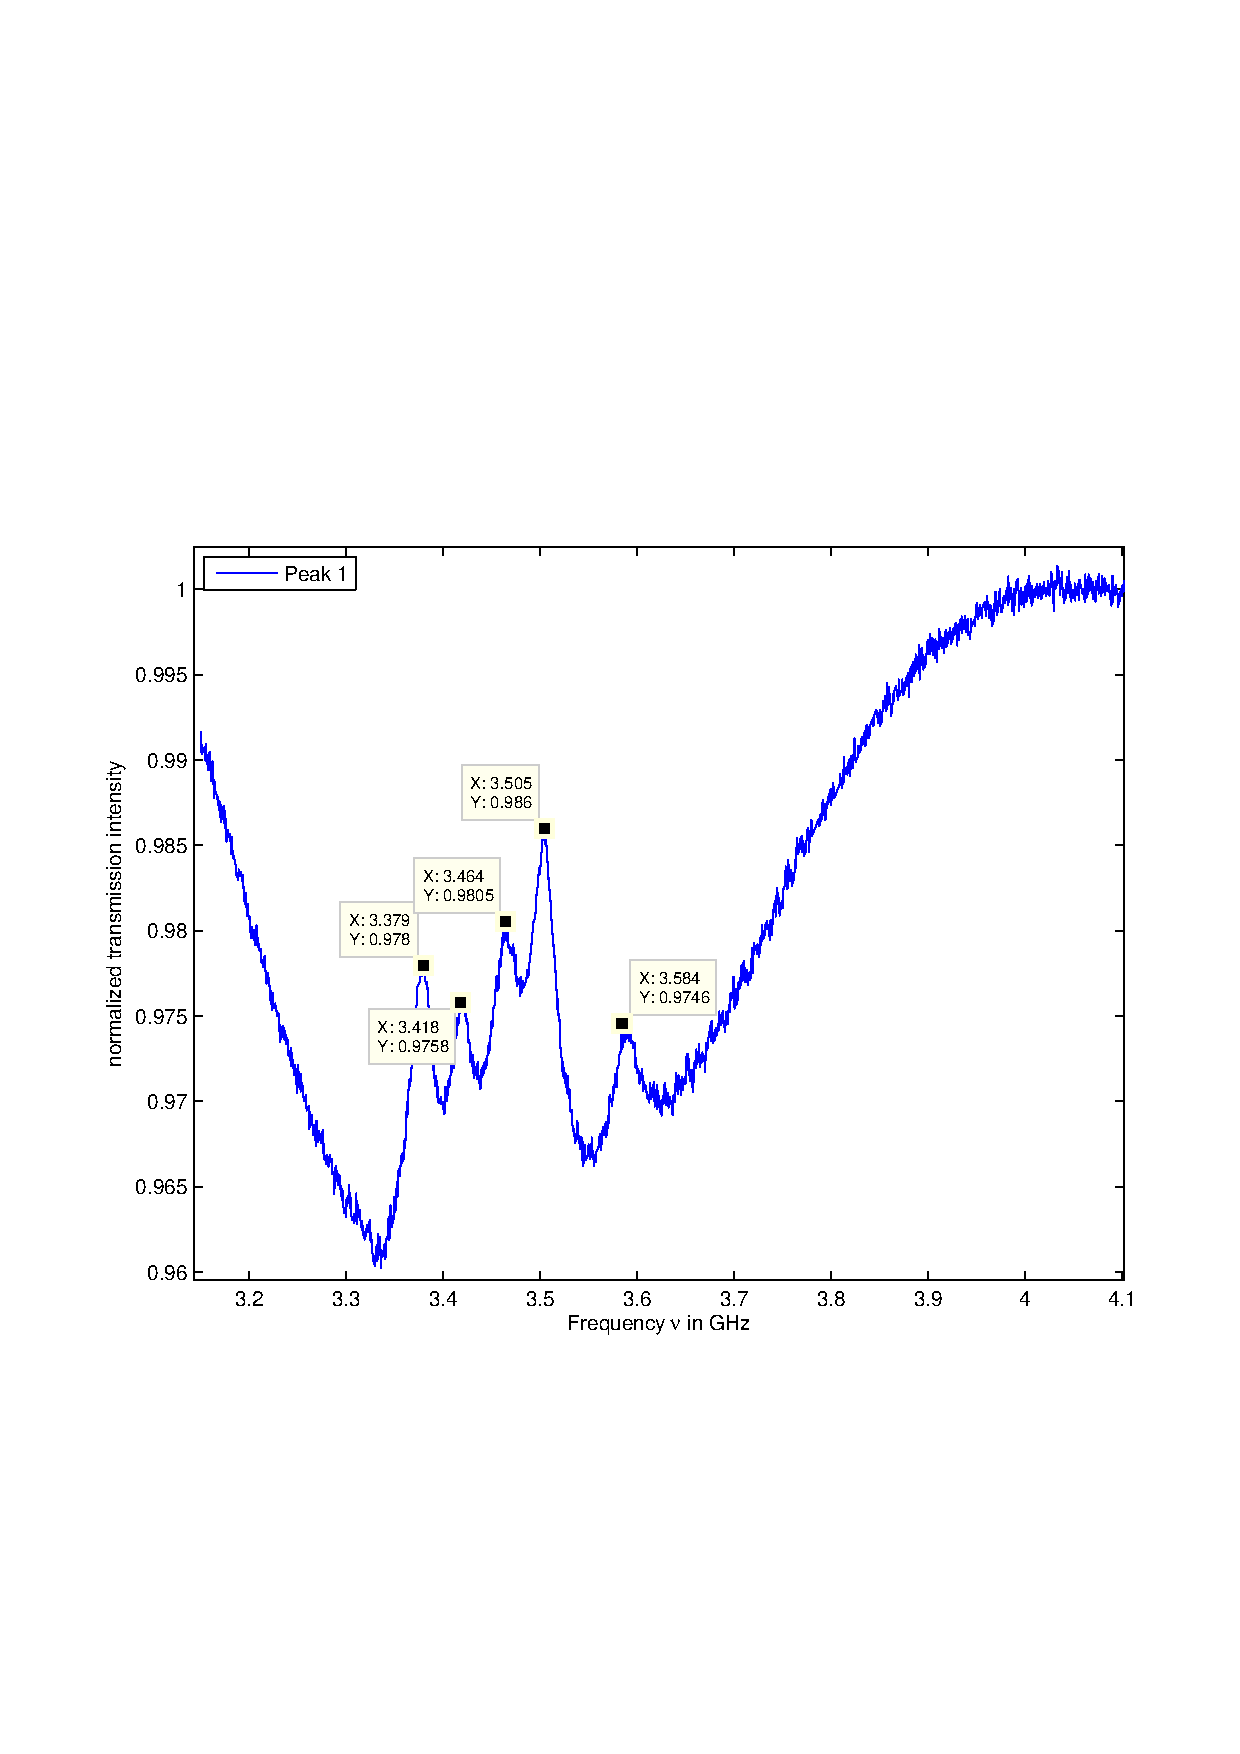
\includegraphics[width=0.9\textwidth, clip, trim=1.5cm 7cm 1.5cm 9cm]{graph/peak1.pdf}
	\vspace{-1ex}
	\caption{Lamb dips on peak 1.}
	\label{fig:P1}
	\vspace{2ex}

	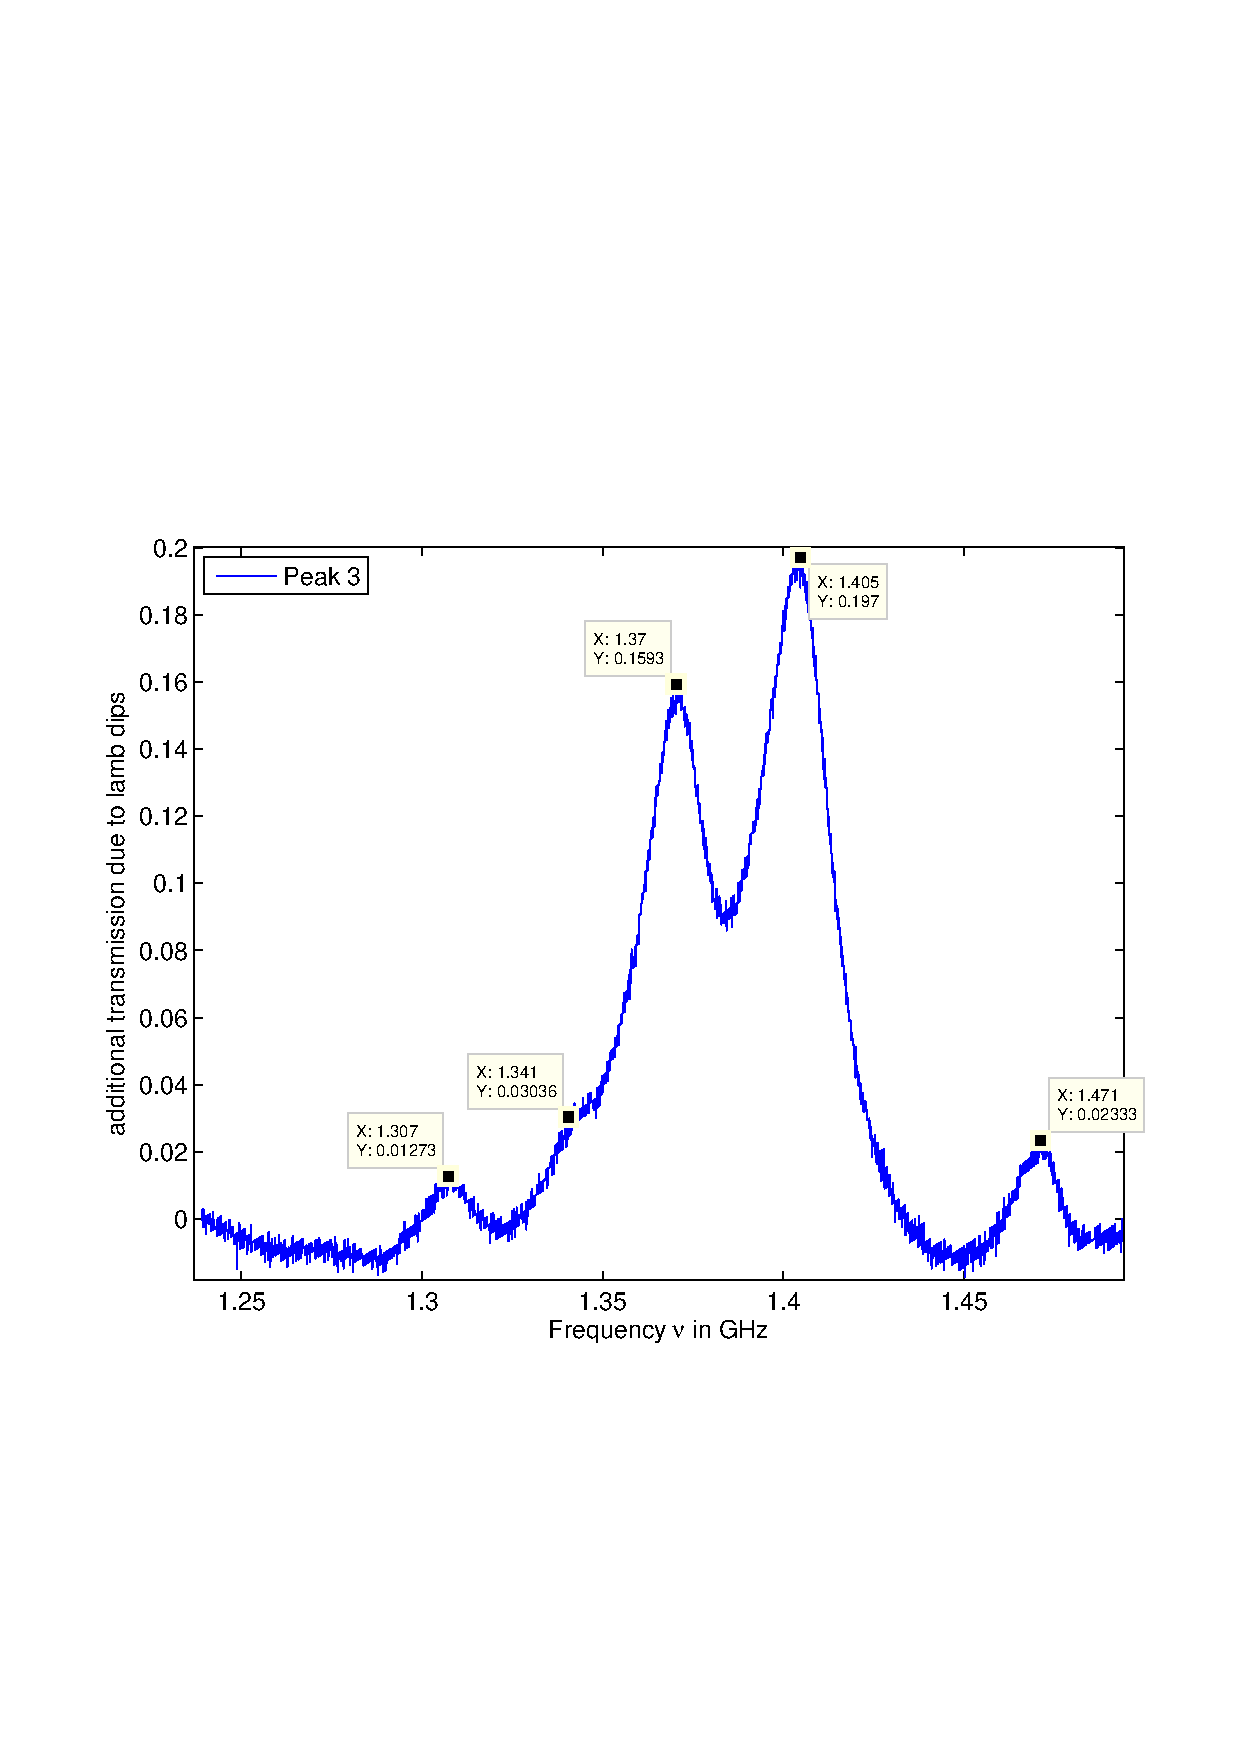
\includegraphics[width=0.9\textwidth, clip, trim=1.5cm 7cm 1.5cm 9cm]{graph/peak3.pdf}
	\vspace{-1ex}
	\caption{Lamb dips on peak 3.}
	\label{fig:P3}
	\vspace{-2em}
\end{figure}

\begin{figure}[p]
	\centering
	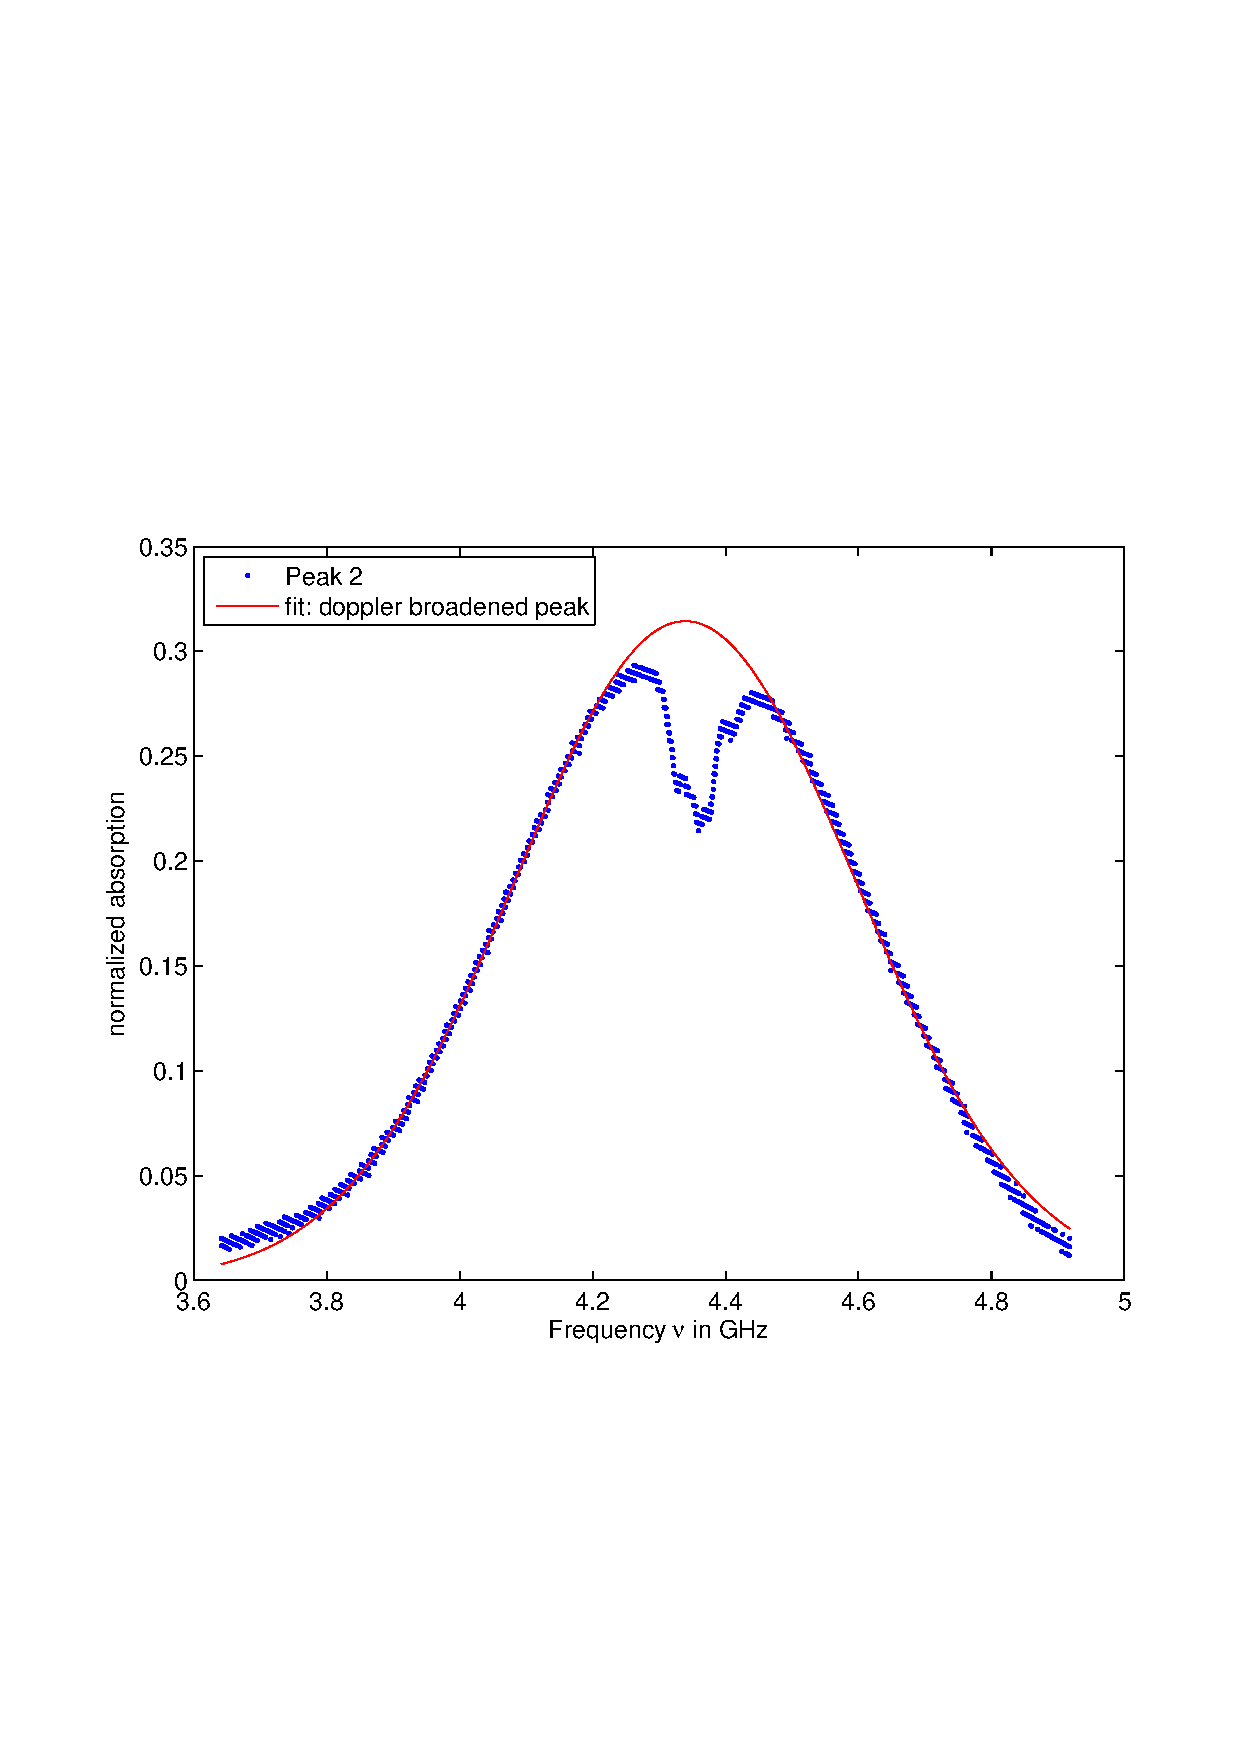
\includegraphics[width=0.9\textwidth, clip, trim=1.5cm 7cm 1.5cm 9cm]{graph/peak2.pdf}
	\vspace{-1ex}
	\caption{Lamb dips on peak 2.}
	\label{fig:P2f}
	\vspace{2ex}

	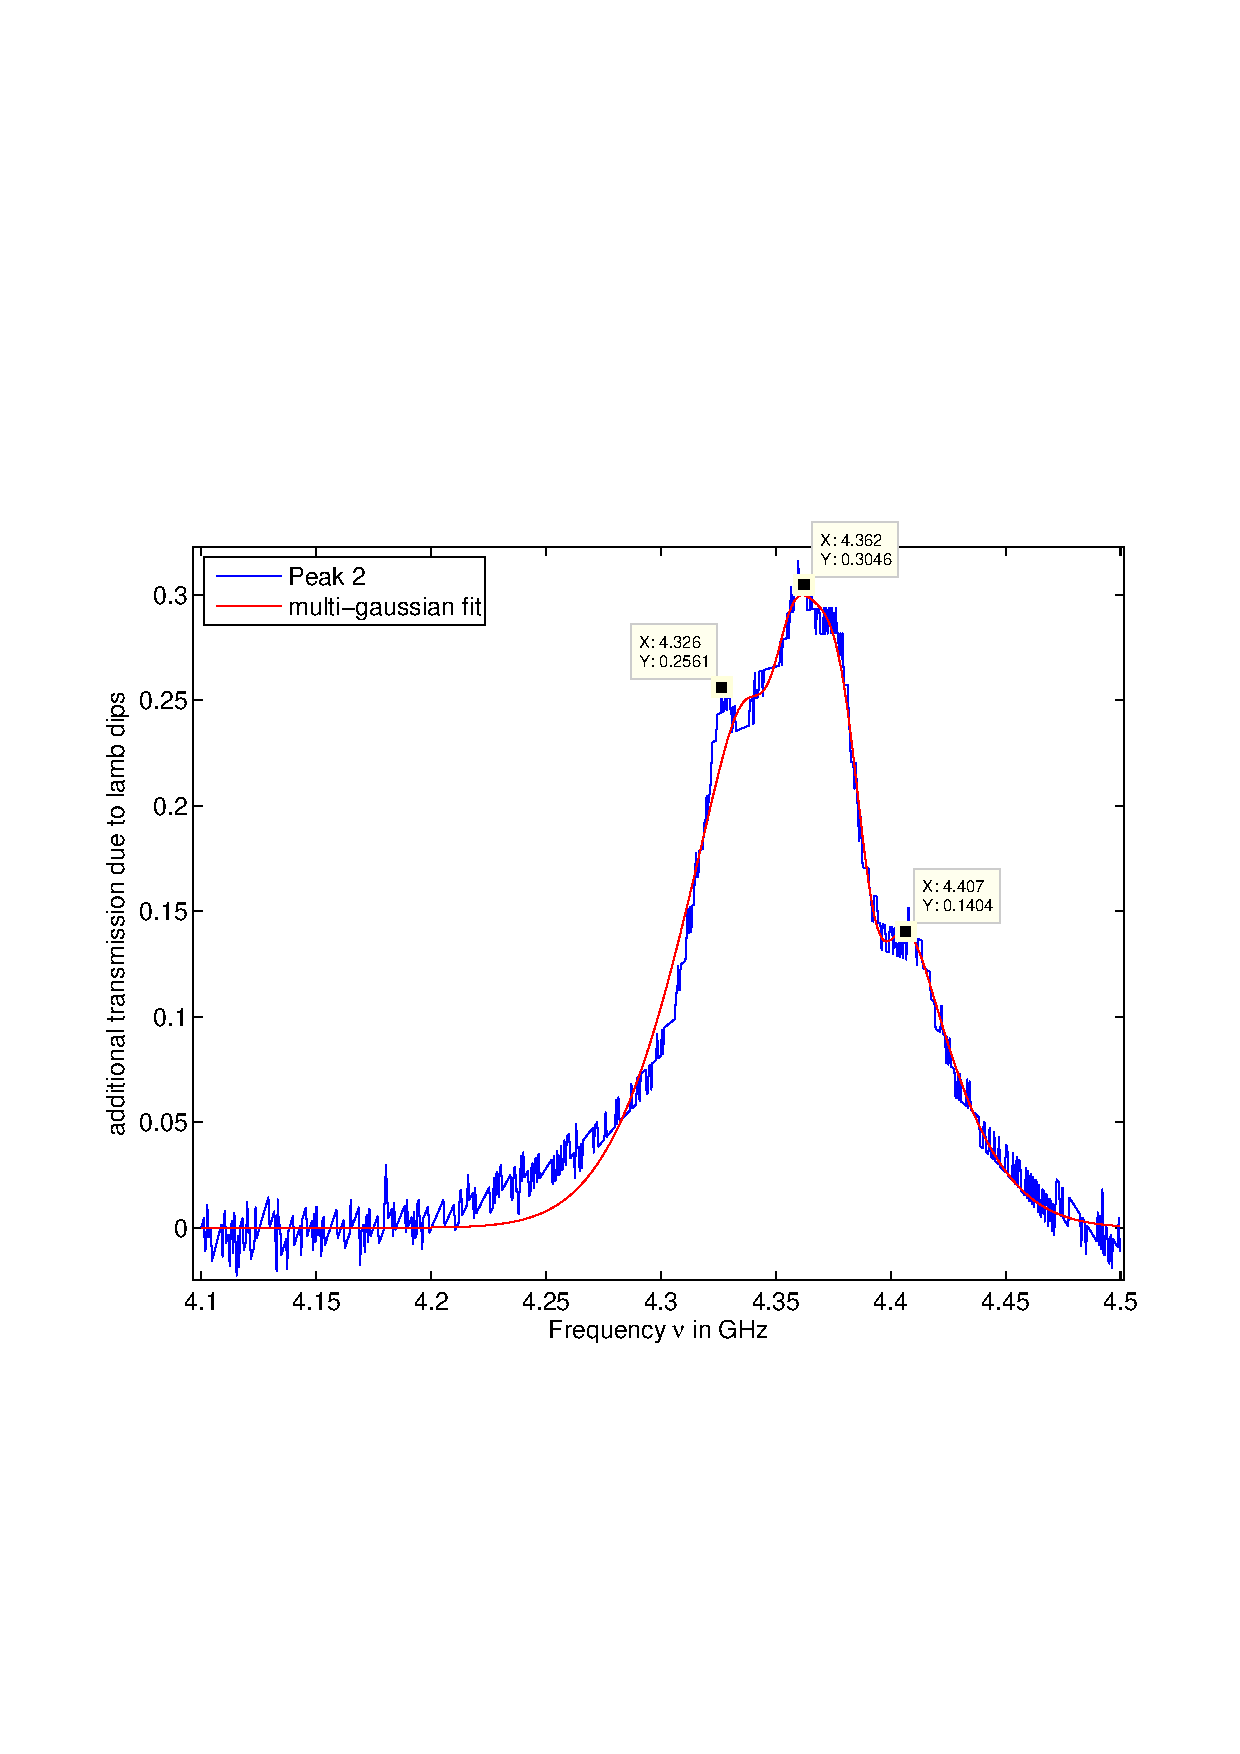
\includegraphics[width=0.9\textwidth, clip, trim=1.5cm 7cm 1.5cm 9cm]{graph/peak2_detail.pdf}
	\vspace{-1ex}
	\caption{Lamb dips on peak 2 after deducting the fit from figure \ref{fig:P2f}.}
	\label{fig:P2}
	\vspace{-2em}
\end{figure}

\begin{figure}[p]
	\centering
	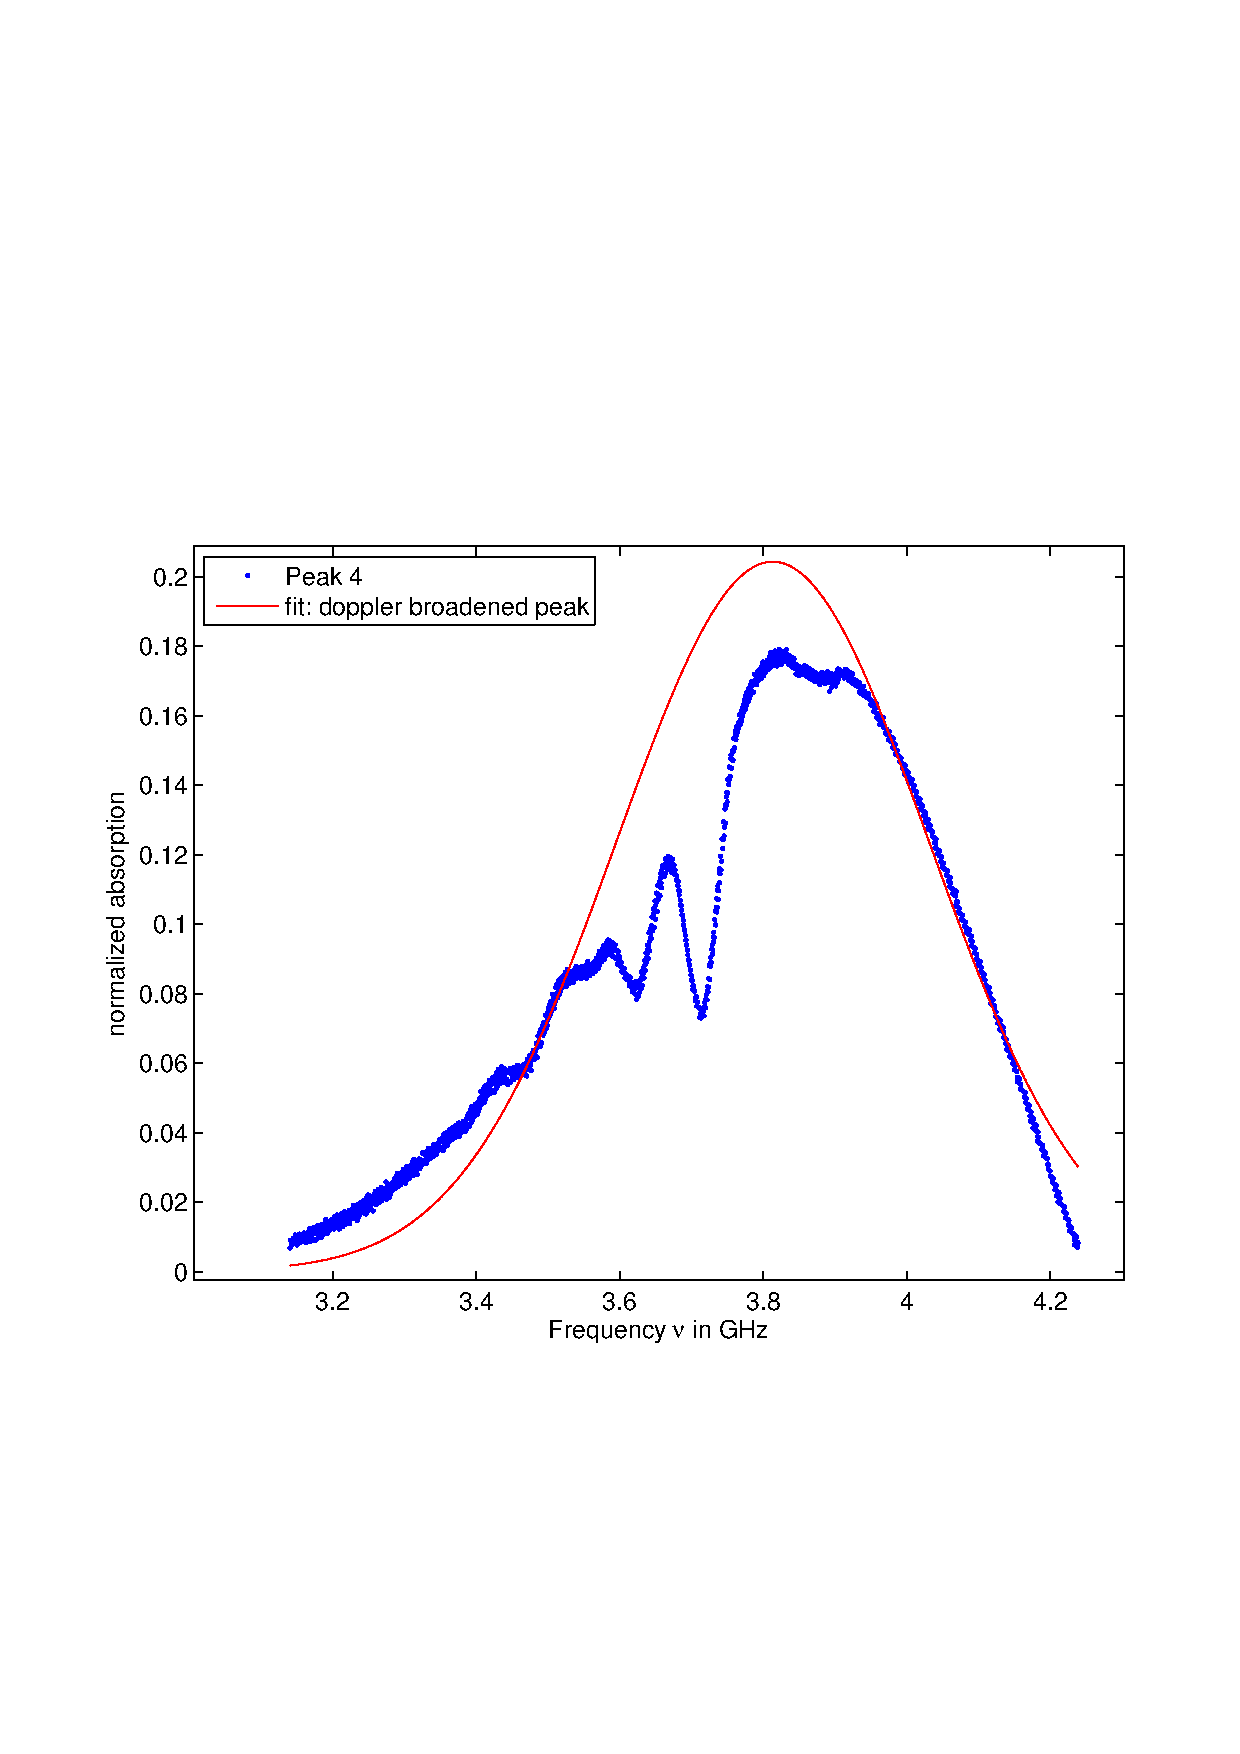
\includegraphics[width=0.9\textwidth, clip, trim=1.5cm 7cm 1.5cm 9cm]{graph/peak4.pdf}
	\vspace{-1ex}
	\caption{Lamb dips on peak 4.}
	\label{fig:P4f}
	\vspace{2ex}

	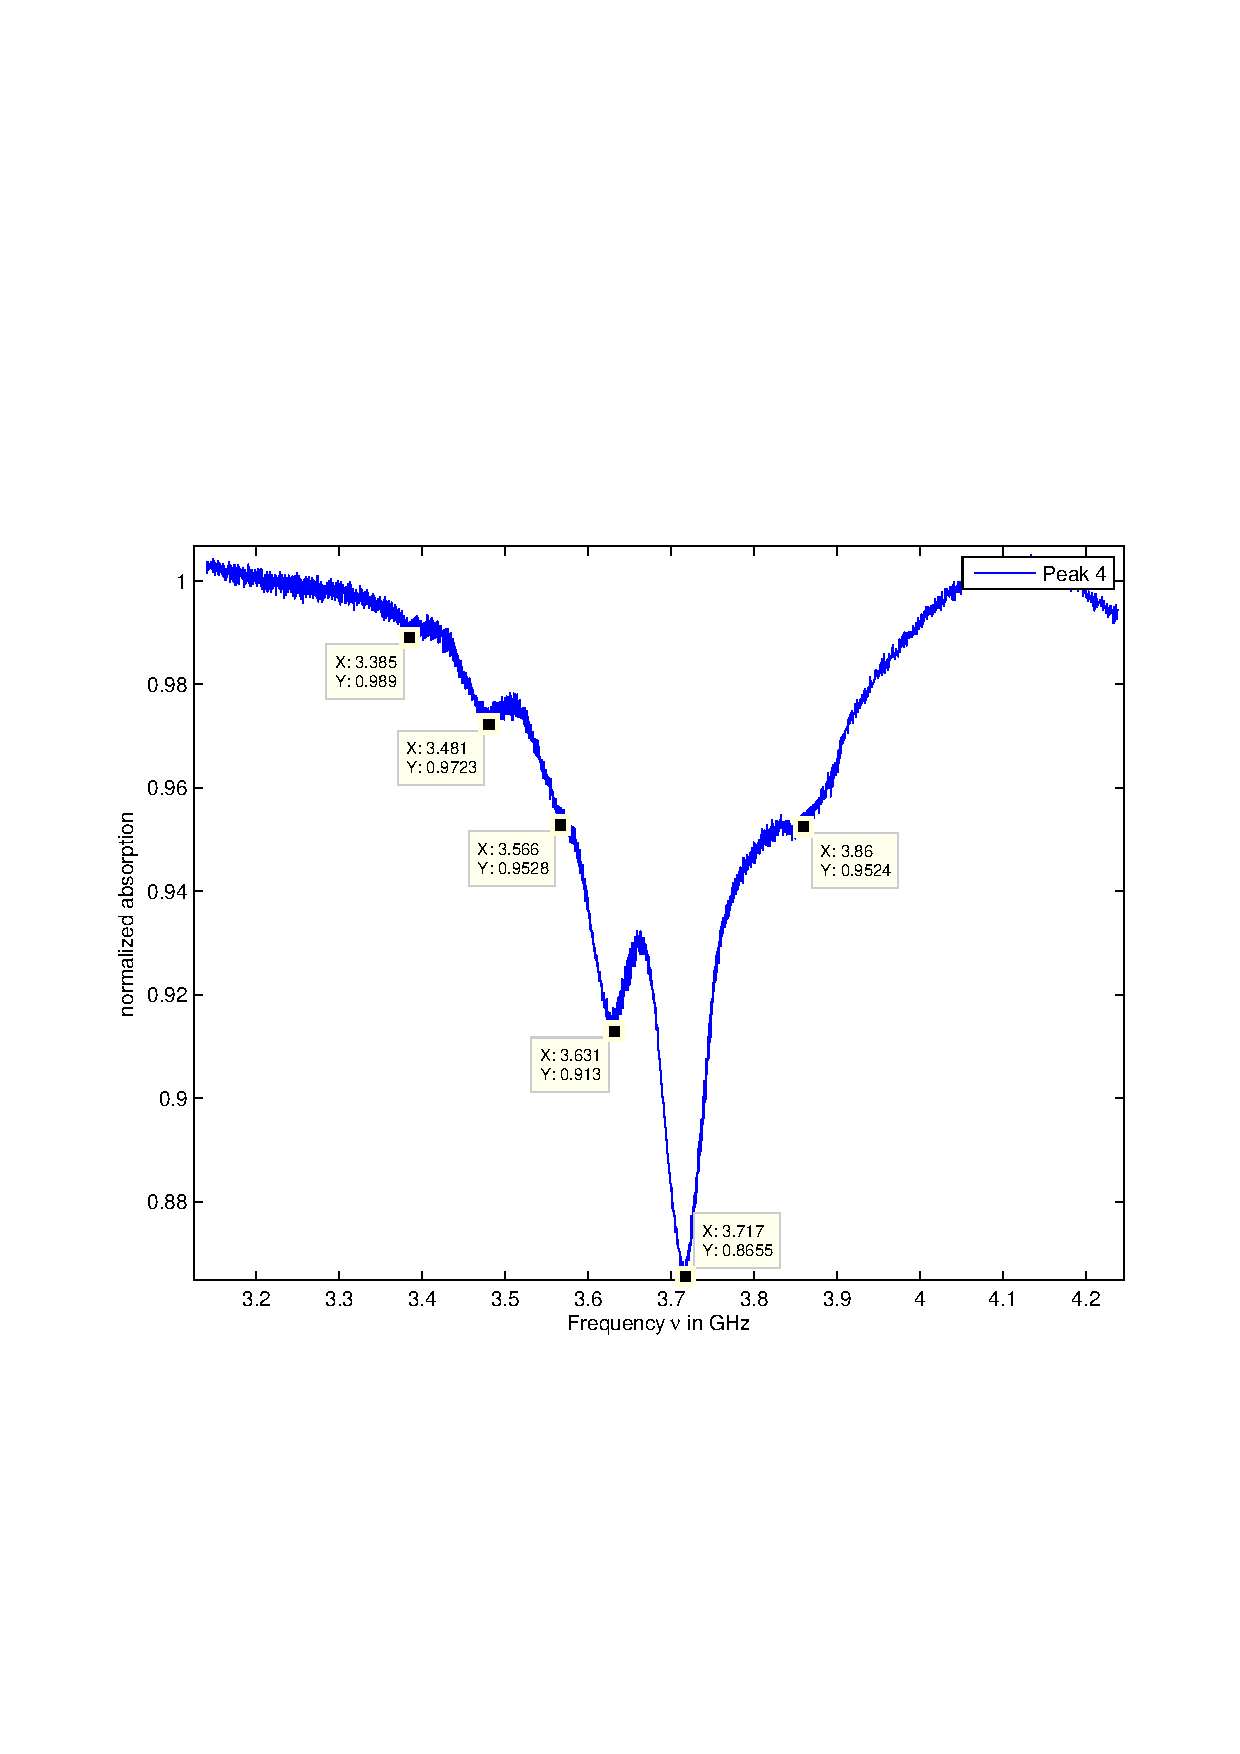
\includegraphics[width=0.9\textwidth, clip, trim=1.5cm 7cm 1.5cm 9cm]{graph/peak4_detail.pdf}
	\vspace{-1ex}
	\caption{Lamb dips on peak 4 after deducting the fit from figure \ref{fig:P4f}.}
	\label{fig:P4}
	\vspace{-2em}
\end{figure}

\newpage
\subsection{Frequency modulation spectroscopy}

As our modulation signal $U_\text{mod}$ has a frequency of 0.1\,MHz and the high-frequency component of $U_\text{mix}$ oscillates with double that frequency, we should use a low pass filter with a cut off frequency of 0.2\,MHz at most. However,  the best filter available to us lets frequencies  up to 2.5\,MHz pass through. As an additional measure, we averaged over multiple trigger periods via the oscilloscope.

This especially has an effect on the already feeble signal from Peak 1 -- part of the modulation signal isn't filtered out and remains as noise, obscuring the data. For Peak 3, the averaging of the oscilloscope had to be deactivated as it averaged out one of the dips.

To rectify this issue, we applied a 5000\,Hz low pass filter as digital post processing for these two peaks. Based on the sample interval $T = 2\,\micro\second$ and the filter time constant $\tau = \frac{1}{2 \pi \cdt 5000\,\hertz}$ we code:

\lstinputlisting[style=mlab, caption={Matlab low pass filter \cite{lit:lowpass}}\label{code:filter}\\
]{./Matlab/lowpass5000.m}

While the low pass filter massively improves the identification of the zero crossings, the method still yields less reliable data compared to the standard saturation spectroscopy. However, this is an issue with the setup we used and not the frequency modulation spectroscopy itself -- correctly done, it can give the most detailed results of the three presented methods.

As to the data analysis, each second zero point doesn't correspond to a lamb dip but to a local absorption maximum

\begin{figure}[p]
	\centering
	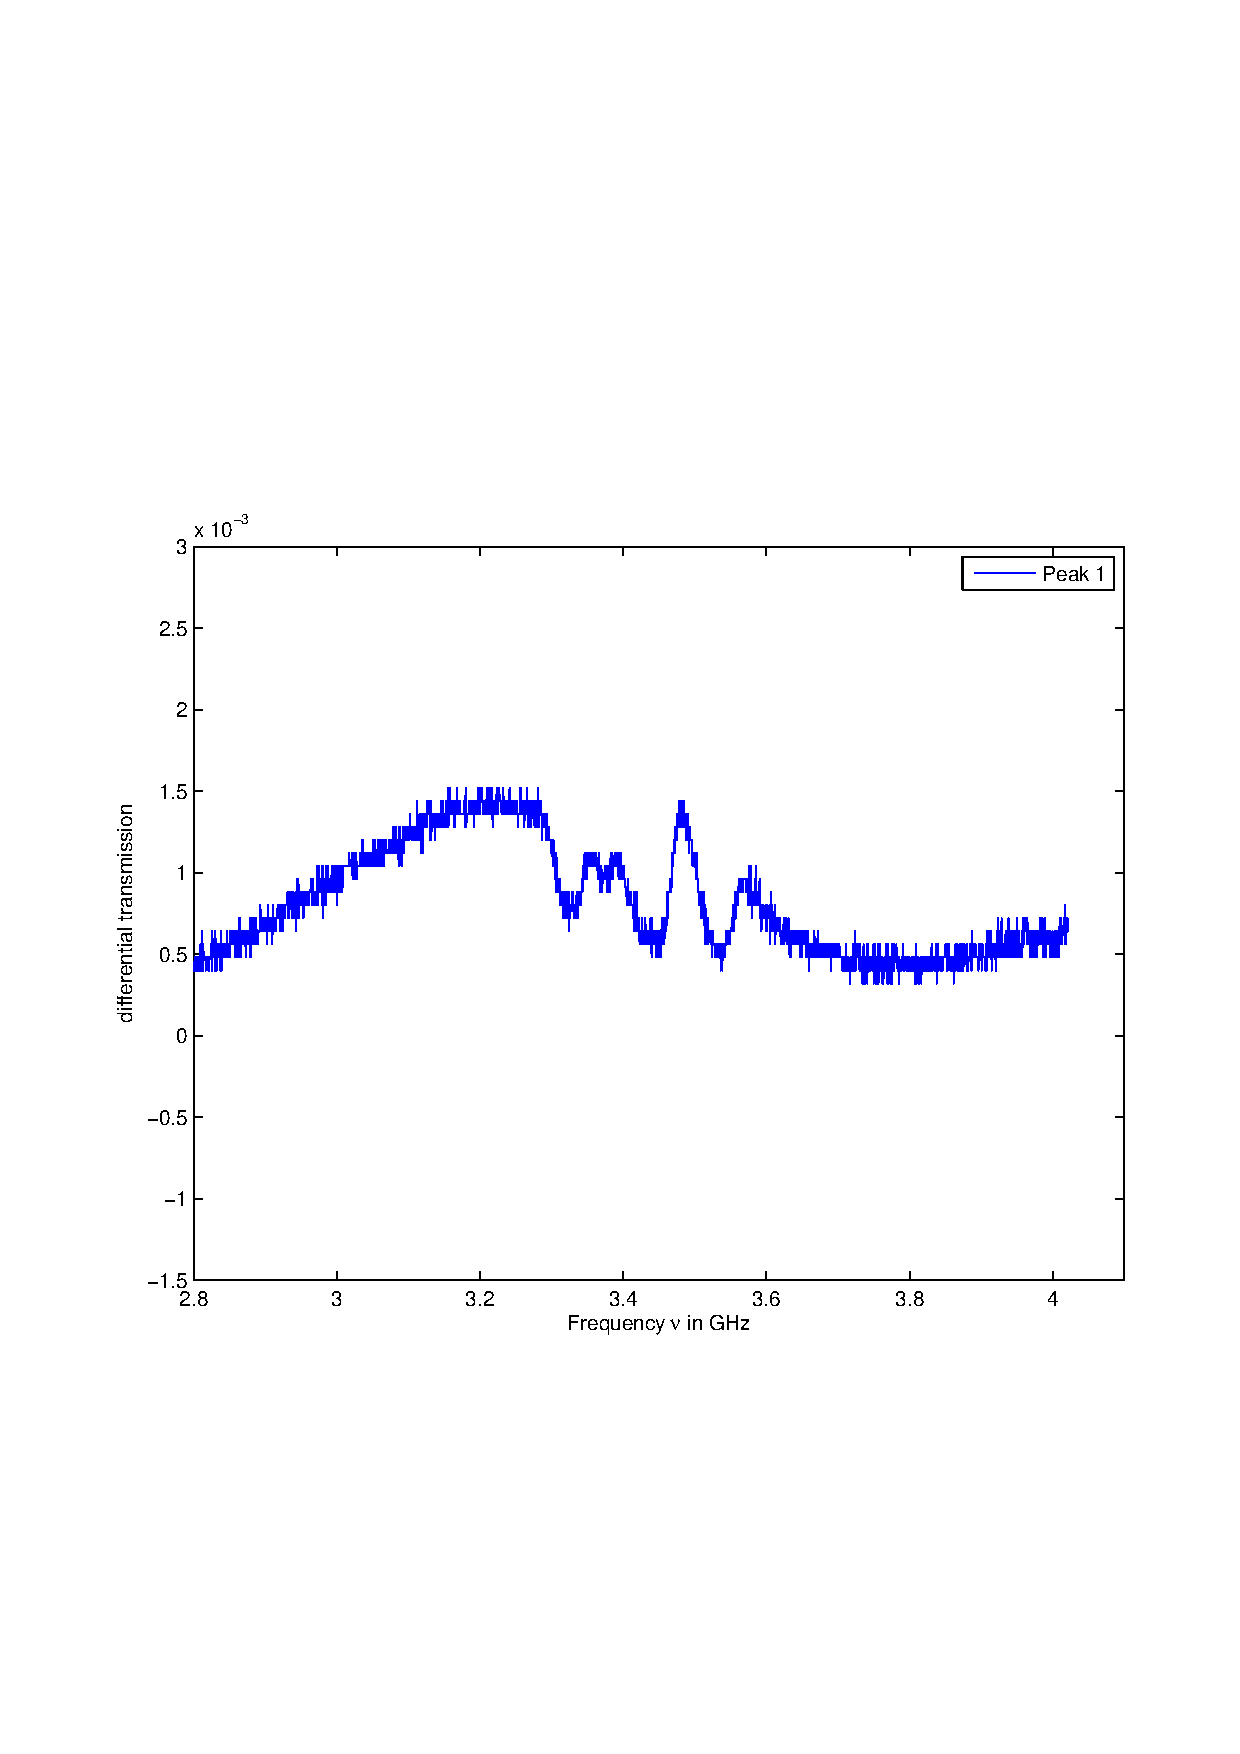
\includegraphics[width=0.9\textwidth, clip, trim=1.5cm 7cm 1.5cm 9cm]{graph/peak1_fms.pdf}
	\vspace{-2ex}
	\caption{FMS Peak 1}
	\label{fig:P1_fms}
	\vspace{2ex}

	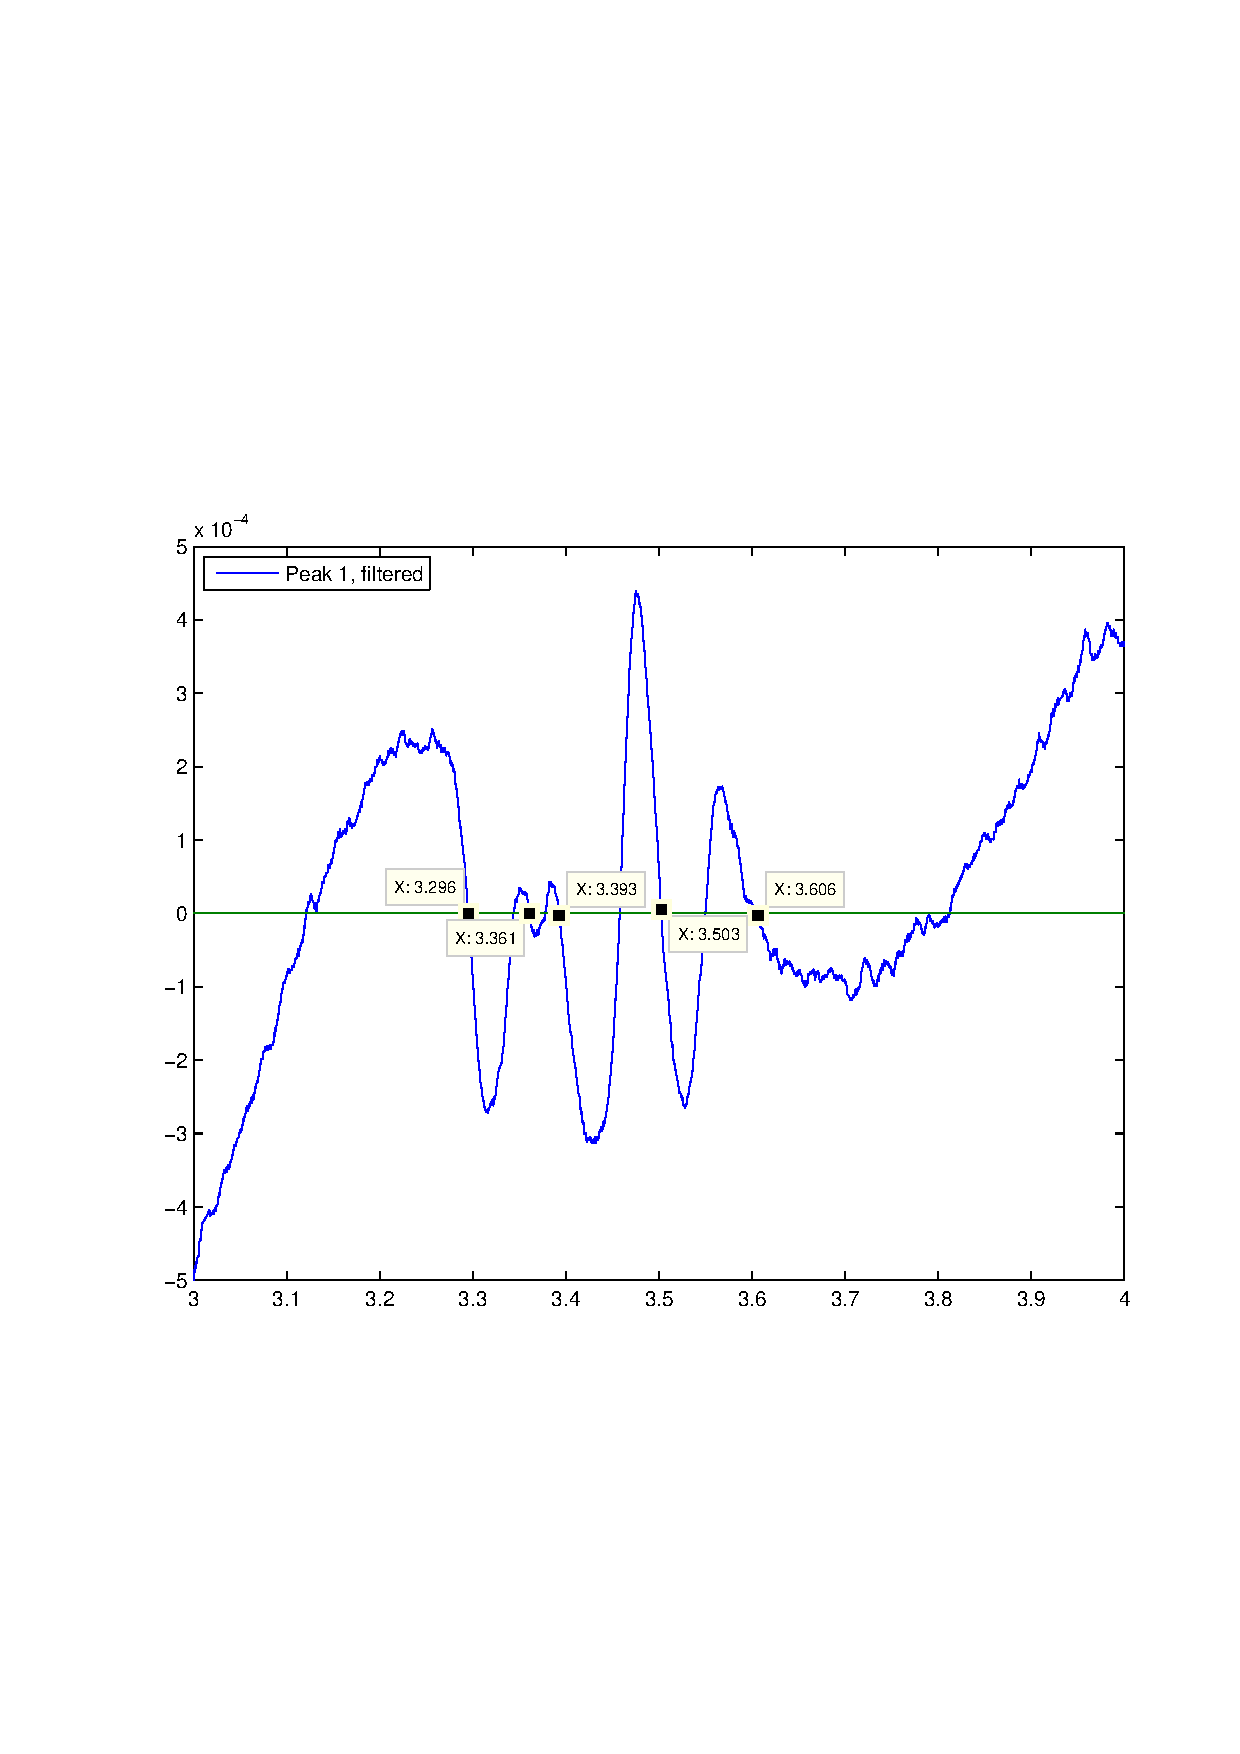
\includegraphics[width=0.9\textwidth, clip, trim=1.5cm 7cm 1.5cm 9cm]{graph/peak1_filter.pdf}
	\vspace{-2ex}
	\caption{FMS Peak 1}
	\label{fig:P1_filter}
	\vspace{-2em}
\end{figure}

\begin{figure}[p]
	\centering
	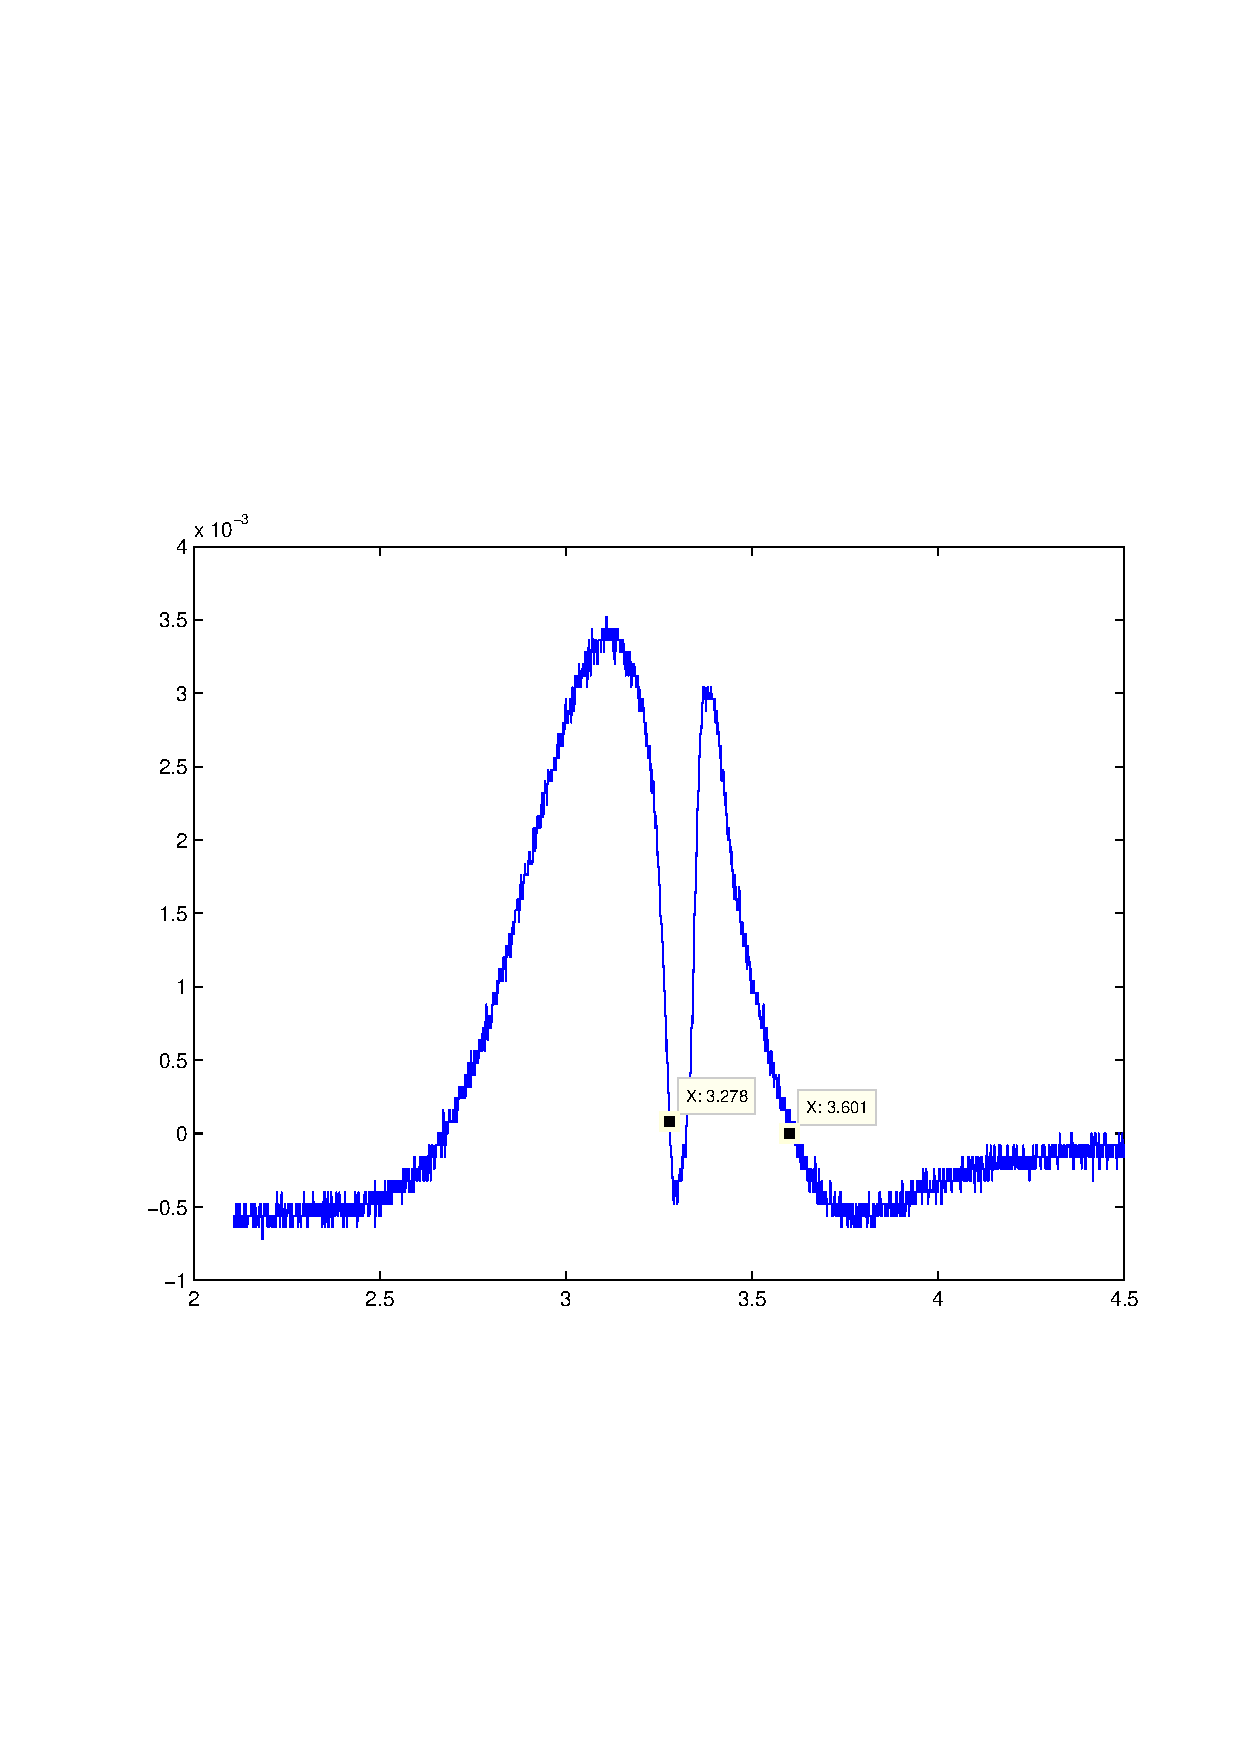
\includegraphics[width=0.9\textwidth, clip, trim=1.5cm 7cm 1.5cm 9cm]{graph/peak2_fms.pdf}
	\vspace{-2ex}
	\caption{FMS Peak 2}
	\label{fig:P2_fms}
	\vspace{2ex}

	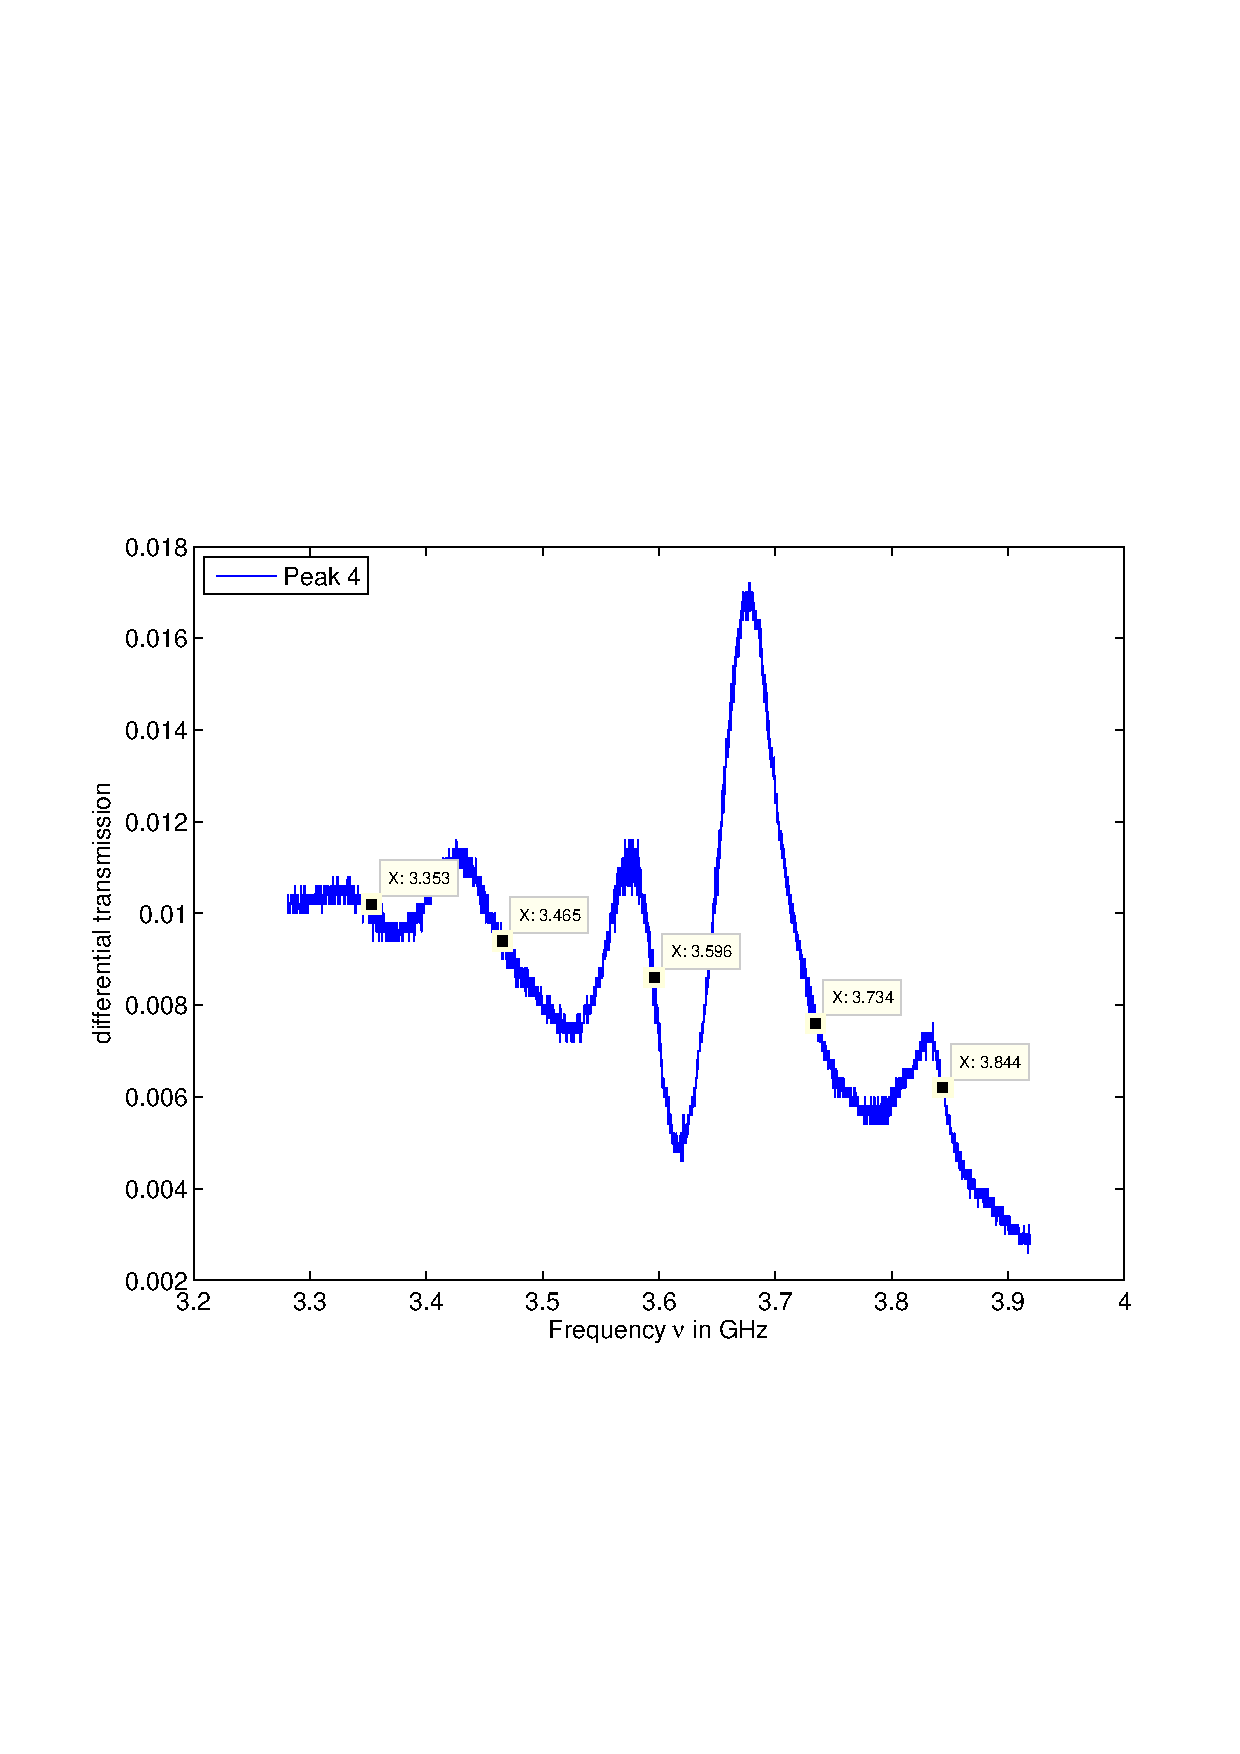
\includegraphics[width=0.9\textwidth, clip, trim=1.5cm 7cm 1.5cm 9cm]{graph/peak4_fms.pdf}
	\vspace{-2ex}
	\caption{FMS Peak 4, the middle data tip was placed accidentally}
	\label{fig:P4_fms}
	\vspace{-2em}
\end{figure}

\begin{figure}[p]
	\centering
	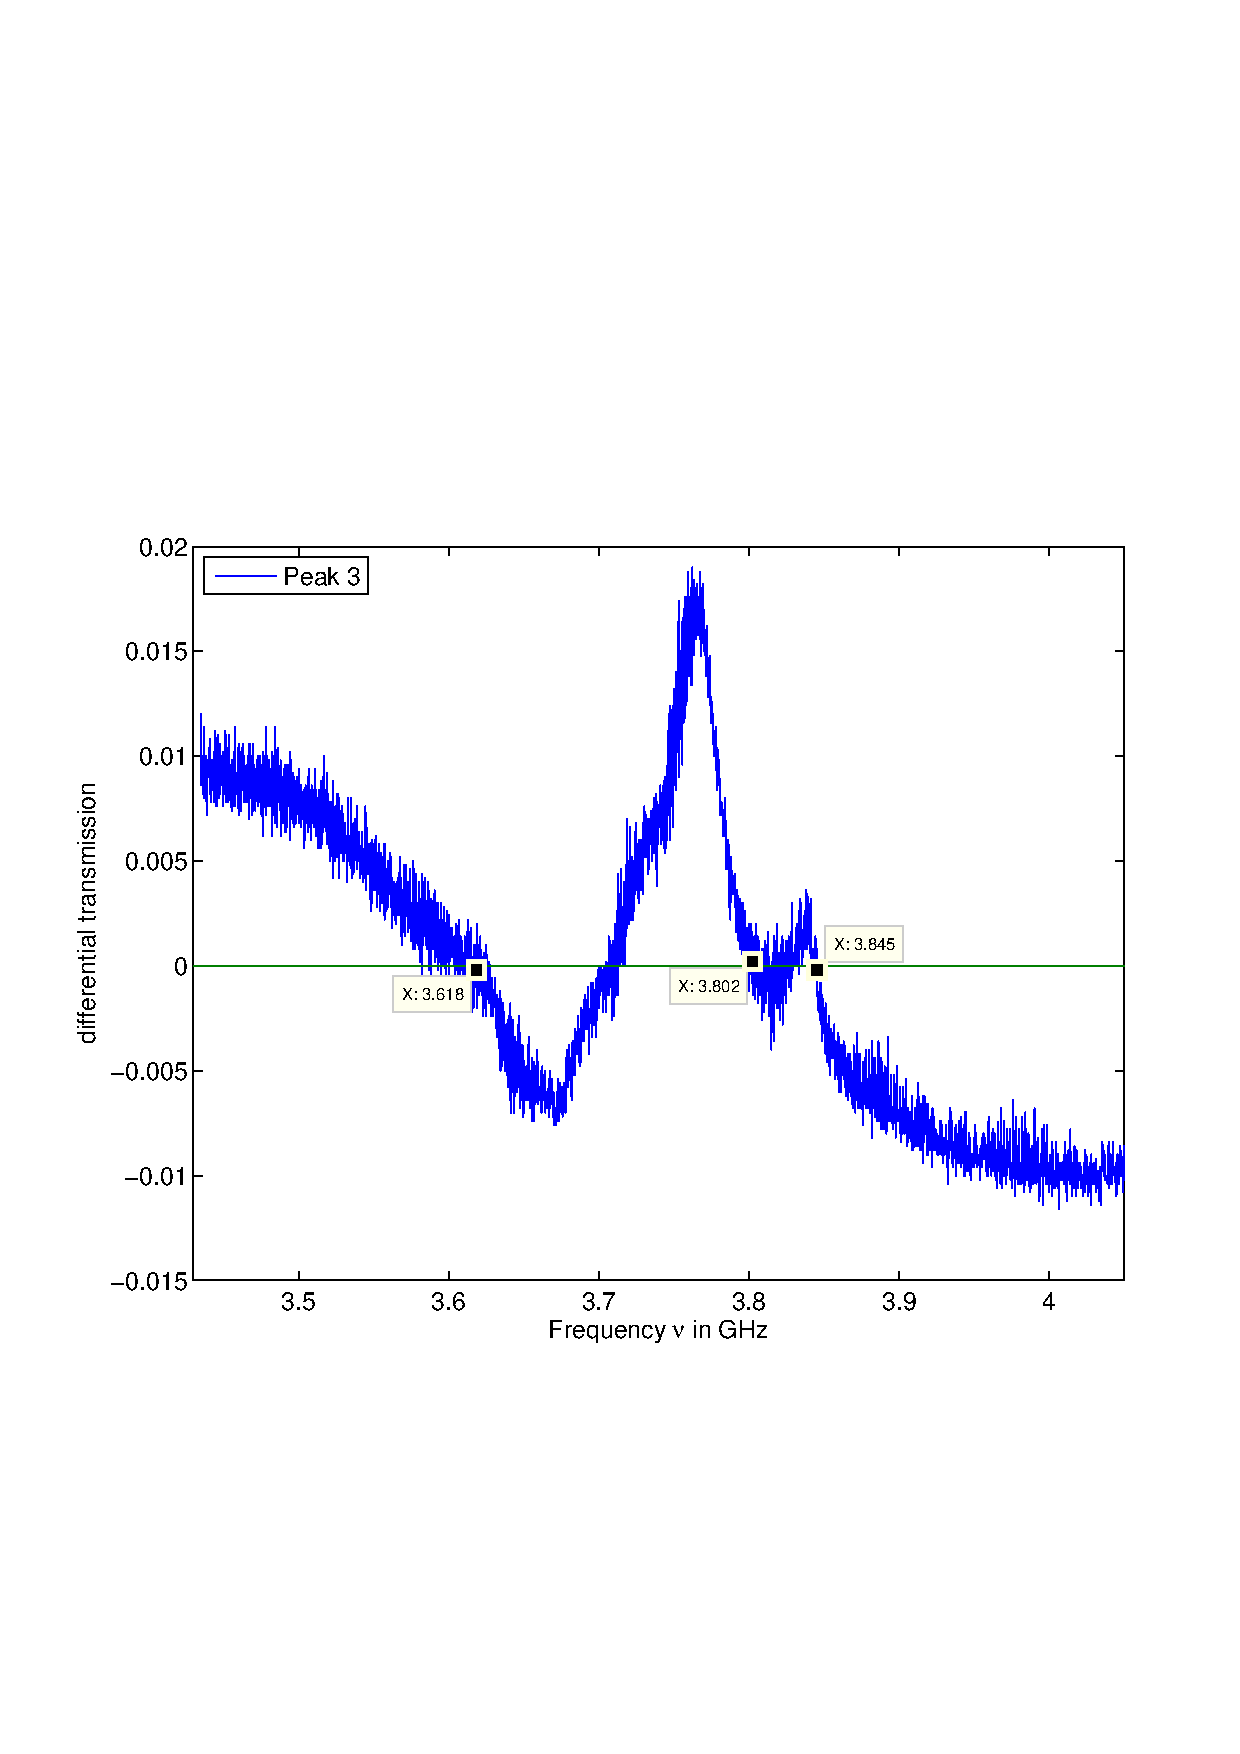
\includegraphics[width=0.9\textwidth, clip, trim=1.3cm 7cm 1.5cm 9cm]{graph/peak3_fms.pdf}
	\vspace{-2ex}
	\caption{FMS Peak 3}
	\label{fig:P3_fms}
	\vspace{2ex}

	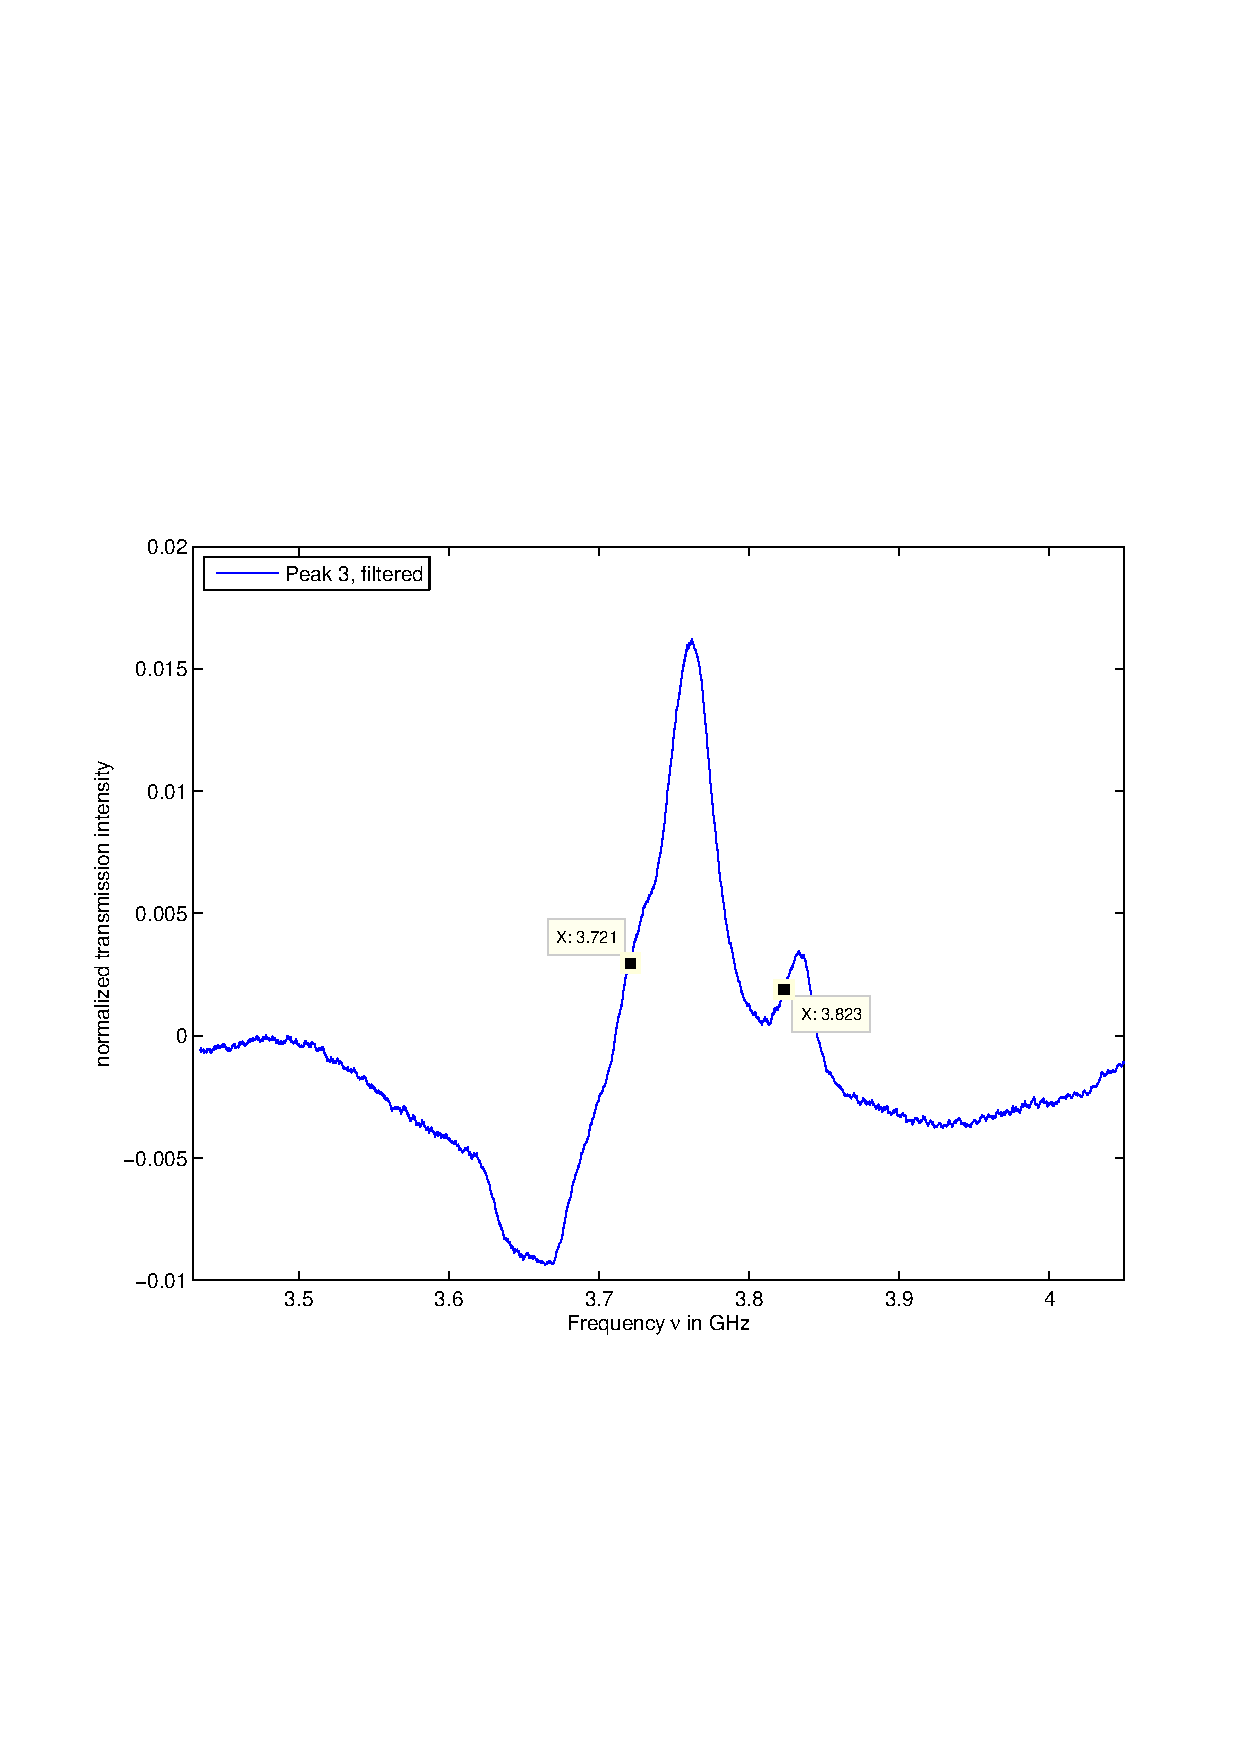
\includegraphics[width=0.9\textwidth, clip, trim=1.3cm 7cm 1.5cm 9cm]{graph/peak3_filter.pdf}
	\vspace{-2ex}
	\caption{FMS Peak 3}
	\label{fig:P3_filter}
	\vspace{-2em}
\end{figure}
